%! TeX program = tectonic
\documentclass[nobib, a4paper]{tufte-book}
\setcounter{tocdepth}{2}
\usepackage{microtype, ifluatex, ifxetex}
%Next block avoids bug, from  http://tex.stackexchange.com/a/200725/1913
\ifx\ifxetex\ifluatex\else % if lua- or xelatex http://tex.stackexchange.com/a/140164/1913
  \usepackage{fontspec}
  \setmainfont[Renderer=Basic, Scale=0.90]{OpenDyslexic}
  \setsansfont[Renderer=Basic, Scale=0.90]{OpenDyslexic}
  \setmonofont[Renderer=Basic]{OpenDyslexicMono}

  \setmainfont[Renderer=Basic, Numbers=OldStyle, Scale = 1.0]{TeX Gyre Pagella}
  \setsansfont[Renderer=Basic, Scale=0.90]{TeX Gyre Heros}
  \setmonofont[Renderer=Basic]{TeX Gyre Cursor}

  % \setmainfont[Mapping=tex-text,Numbers=OldStyle]{Bembo Std}
  % \setsansfont[Mapping=tex-text,Numbers=OldStyle,Scale=MatchLowercase]{Gill Sans}
  % \setmonofont[Mapping=tex-text,Scale=MatchLowercase]{DejaVu Sans Mono}

  \renewcommand{\textls}[2][5]{%
    \begingroup\addfontfeatures{LetterSpace=#1}#2\endgroup
  }
  \renewcommand{\allcapsspacing}[1]{\textls[15]{#1}}
  \renewcommand{\smallcapsspacing}[1]{\textls[10]{#1}}
  \renewcommand{\allcaps}[1]{\textls[15]{\MakeTextUppercase{#1}}}
  \renewcommand{\smallcaps}[1]{\smallcapsspacing{\scshape\MakeTextLowercase{#1}}}
  \renewcommand{\textsc}[1]{\smallcapsspacing{\textsmallcaps{#1}}}
\fi

\usepackage{graphicx} % allow embedded images
\setkeys{Gin}{width=\linewidth,totalheight=\textheight,keepaspectratio}
\graphicspath{{images/}} % set of paths to search for images
\usepackage{amsmath,amssymb,amsthm,amsfonts}  % extended mathematics
\usepackage[normalem]{ulem}
\usepackage{booktabs} % book-quality tables
\usepackage{units}    % non-stacked fractions and better unit spacing
\usepackage{multicol} % multiple column layout facilities
\usepackage{fancyvrb} % extended verbatim environments
\fvset{fontsize=\normalsize}% default font size for fancy-verbatim environments
\usepackage{tikz,tikz-cd,quiver,mathbbol}
\DeclareSymbolFontAlphabet{\mathbbl}{bbold} %let's you use \mathbbl{k} for a field k
\setcounter{secnumdepth}{2}
\usepackage{enumerate}
\usepackage{mathabx}
\usepackage{mathtools}
\mathtoolsset{showonlyrefs, mathic}
\usepackage[english]{babel}
\usepackage{hyperref}
\hypersetup{
  colorlinks=true,
  urlcolor=Cerulean,
  linkcolor = ForestGreen,
}
\usepackage[toc]{appendix}

\newcounter{dummy} %so that \pageref works properly
\usepackage[absolute]{textpos}
\setlength{\TPHorizModule}{\paperwidth} \setlength{\TPVertModule}{\paperheight}


\usetikzlibrary{decorations.pathreplacing,} %for braces with itemize
\newcommand{\tikzmark}[1]{\tikz[baseline={(#1.base)},overlay,remember picture] \node[outer sep=0pt, inner sep=0pt] (#1) {\phantom{A}};}
\usetikzlibrary{cd}

% Standardize command font styles and environments
\newcommand{\doccmd}[1]{\texttt{\textbackslash#1}}% command name -- adds backslash automatically
\newcommand{\docopt}[1]{\ensuremath{\langle}\textrm{\textit{#1}}\ensuremath{\rangle}}% optional command argument
\newcommand{\docarg}[1]{\textrm{\textit{#1}}}% (required) command argument
\newcommand{\docenv}[1]{\textsf{#1}}% environment name
\newcommand{\docpkg}[1]{\texttt{#1}}% package name
\newcommand{\doccls}[1]{\texttt{#1}}% document class name
\newcommand{\docclsopt}[1]{\texttt{#1}}% document class option name
\newenvironment{docspec}{\begin{quote}\noindent}{\end{quote}}% command specification environment

\newcommand{\adj}[4]{\begin{tikzcd}[ampersand replacement=\&, column sep=4ex]
    #1 \colon #2	\ar[yshift=+.6ex]{r}
    \& #3 \colon #4	\ar[yshift=-.4ex]{l}
\end{tikzcd}}

\usepackage{etoolbox}
\newcommand{\addQEDstyle}[2]{
  \AtBeginEnvironment{#1}{\pushQED{\qed}\renewcommand{\qedsymbol}{#2}}
  \AtEndEnvironment{#1}{\popQED}
}

\theoremstyle{plain}
\newtheorem{theorem}{Theorem}[section]
\newtheorem{corollary}[theorem]{Corollary}
\newtheorem{proposition}[theorem]{Proposition}
\newtheorem{lemma}[theorem]{Lemma}

\theoremstyle{definition}
\newtheorem{definition}[theorem]{Definition}
\addQEDstyle{definition}{$\lozenge$}
\newtheorem{conjecture}[theorem]{Conjecture}
\addQEDstyle{conjecture}{$\clubsuit$}

\theoremstyle{remark}
\newtheorem{example}[theorem]{Example}
\addQEDstyle{example}{$\lozenge$}
\newtheorem{remark}[theorem]{Remark}
\addQEDstyle{remark}{$\lozenge$}
\newtheorem{notation}[theorem]{Notation}
\addQEDstyle{notation}{$\lozenge$}

\usepackage{oplotsymbl}
\newtheorem{exercise}[theorem]{Exercise}
\addQEDstyle{exercise}{$\starlet$}
\newtheorem{problem}[theorem]{Problem}
\addQEDstyle{problem}{$\starlet$}

\usepackage[
type={CC},
modifier={by-nc-sa},
version={4.0},
]{doclicense}

\usepackage[dvipsnames]{xcolor}
\usepackage[many]{tcolorbox}

%\usepackage[numbers, sort]{natbib}
\usepackage[style=alphabetic,natbib=true,sorting=anyt]{biblatex}
%\setlength{\bibsep}{3pt}
%\renewcommand{\bibfont}{\small}
\usepackage{doi}
\addbibresource{aom.bib}

\usepackage{makeidx}
\makeindex

\newcommand{\cA}{\mathcal{A}}
\newcommand{\cC}{\mathcal{C}}
\newcommand{\cD}{\mathcal{D}}
\newcommand{\cE}{\mathcal{E}}
\newcommand{\cF}{\mathcal{F}}
\newcommand{\cL}{\mathcal{L}}
\newcommand{\cO}{\mathcal{O}}
\newcommand{\cH}{\mathcal{H}}
\newcommand{\cI}{\mathcal{I}}
\newcommand{\cT}{\mathcal{T}}
\newcommand{\cB}{\mathcal{B}}
\newcommand{\cU}{\mathcal{U}}
\newcommand{\cX}{\mathcal{X}}

%\newcommand{\bC}{\mathbb{C}}
\newcommand{\N}{\mathbb{N}}
\newcommand{\Z}{\mathbb{Z}}
\newcommand{\Q}{\mathbb{Q}}
\newcommand{\R}{\mathbb{R}}
\newcommand{\RP}{\mathbb{RP}}
\newcommand{\bS}{\mathbb{S}}
\newcommand{\bT}{\mathbb{T}}

\newcommand{\fX}{\mathfrak{X}}
\newcommand{\fg}{\mathfrak{g}}
\newcommand{\fh}{\mathfrak{h}}

\newcommand{\bx}{\bm{x}}
\newcommand{\bp}{\bm{p}}
\newcommand{\bv}{\bm{v}}

\DeclareFontFamily{U}{MnSymbolC}{}
\DeclareSymbolFont{MnSyC}{U}{MnSymbolC}{m}{n}
\DeclareFontShape{U}{MnSymbolC}{m}{n}{
  <-6>  MnSymbolC5
  <6-7>  MnSymbolC6
  <7-8>  MnSymbolC7
  <8-9>  MnSymbolC8
  <9-10> MnSymbolC9
  <10-12> MnSymbolC10
<12->   MnSymbolC12}{}
\DeclareMathSymbol{\iprod}{\mathbin}{MnSyC}{'270}

\let\d\relax
\DeclareMathOperator{\d}{d}
\DeclareMathOperator{\D}{D}
\DeclareMathOperator{\diff}{Diff}
\DeclareMathOperator{\Id}{Id}
\DeclareMathOperator{\id}{id}
\DeclareMathOperator{\diag}{diag}
\let\mod\relax
\DeclareMathOperator{\mod}{mod}
\DeclareMathOperator{\curl}{curl}
\DeclareMathOperator{\Vol}{Vol}
\DeclareMathOperator{\eval}{eval}
\DeclareMathOperator{\supp}{supp}
\DeclareMathOperator{\sgn}{sgn}

\DeclareMathOperator{\Alt}{Alt}

\DeclareMathOperator{\ad}{ad}
\DeclareMathOperator{\Ad}{Ad}

\newcommand{\todo}[1]{\footnote{\textcolor{red}{#1}}}
\newcommand{\TODO}{\textcolor{red}{\hrulefill}}

\usepackage{etoolbox}
\ifcsdef{LaTeXunderbrace}{}{
\newcommand{\LaTeXunderbrace}[2]{\underbrace{#1}_{#2}}
\newcommand{\LaTeXoverbrace}[2]{\overbrace{#1}^{#2}}
}

\newcommand{\idx}[1]{\index{#1}}
\newcommand{\idxdef}[1]{\index{Definitions!#1}}
\newcommand{\idxthm}[1]{\index{Theorems!#1}}

\title{Analysis\\ \noindent
  on\\ \noindent
  Manifolds
}
\author{Marcello Seri}
\publisher{Bernoulli Institute\\ \noindent
  %A.Y. 2022--2023\\ \noindent
  \MakeLowercase{\texttt{m.seri@rug.nl}}
}

\begin{document}
\maketitlepage

\newpage

\begin{fullwidth}
	~\vfill
	\thispagestyle{empty}
	\setlength{\parindent}{0pt}
	\setlength{\parskip}{\baselineskip}
	Copyright \copyright\ \the\year\ \thanklessauthor

	\par Version 1.6.6 -- \today

	\vfill
	\small{\doclicenseThis}
\end{fullwidth}

\pagenumbering{roman}
\tableofcontents
\cleardoublepage

\pagenumbering{arabic}
\chapter*{Introduction}
\addcontentsline{toc}{chapter}{Introduction}

At the entry for \emph{Mathematical analysis}, our modern source of truth---Wikipedia---says

\begin{quotation}
	\emph{Mathematical analysis} is the branch of mathematics dealing with limits and related theories, such as differentiation, integration, measure, infinite series, and analytic functions.

	These theories are usually studied in the context of real numbers and functions. Analysis evolved from calculus, which involves the elementary concepts and techniques of analysis. Analysis may be distinguished from geometry; however, it can be applied to any space of mathematical objects that has a definition of nearness (a topological space) or specific distances between objects (a metric space).
\end{quotation}

\newthought{In this sense}, our course will focus on generalizing the concepts of differentiation, integration and, up to some extent, differential equations to spaces that are more general than the standard Euclidean space.
We will do this by trying to make everything look Euclidean and, in this sense, the Euclidean space $\R^n$ is going to be \emph{the} prototype of all manifolds: it won't just be our simplest example, we will see that locally every manifold looks like a Euclidean space.

Euclidean spaces, and the Riemannian charts that you may have already encountered in the Geometry course, have a very strong property: they can be described with a set of \emph{global} coordinates.
Even though this means that all computations are explicit, it does make it harder to distinguish \emph{intrinsic}\footnote{I.e. independent from the choice of coordinates.} concepts.
Manifolds will force our hand to work in a \emph{coordinate-free} setting and isolate these intrinsic concepts.
We will see that this will unleash a surprising power that will allow us to lay the foundation for a lot of the mathematics that will come in the rest of the curriculum.

These notes will focus on fundamental ideas of differential geometry, in particular we will discuss manifolds, differential forms, integration, with a wink to the study of vector fields as dynamical systems and topology via cohomology.
If the time permits it, we may give a brief tour of Lie groups and Lie algebras, Riemannian metrics and the notion of curvature, or distributions and Frobenius theorem, depending on the preferences expressed in class.
Some of these topics are already present in appendices to the notes, other will be progressively added in due course.
Throughout the course and these notes, I will try to give particular emphasis on the usefulness of these topics in the mathematics of mechanics and their relevance in certain aspects of topology and field theory.

The course relies \emph{heavily} on your knowledge of linear and multilinear algebra, multivariable analysis and dynamical systems.
This should not come as a surprise: differential geometry studies the natural space in which analysis, in the sense of derivation and integration, can be performed, and was born together with classical mechanics, somehow as unique discipline, before these started diverging on their own paths.

An old mathematical joke says that
\begin{quote}
	differential geometry is the study of properties that are invariant under change of notation.
\end{quote}
Sadly, this is \emph{funny because it is alarmingly close to the truth}\footnote{Cit. Lee~\cite{book:lee}.}.

You will soon see that different references use different notations for just about everything we are going to discuss.
I'll try to stick to the ones you used in the past courses when possible, falling back to~\cite{book:lee} and~\cite{book:tu} and to my personal preference when the latter disagree.

\newthought{These lecture notes} are by no means comprehensive.
As complementary sources you can use the textbook~\cite{book:tu} or the extensive reference~\cite{book:lee}.
You should have access to both books via the University library and, in addition, Lee's ebook can be downloaded via the University proxy on \href{https://link.springer.com/book/10.1007/978-1-4419-9982-5}{SpringerLink}.

The book~\cite{book:McInerney} is a nice compact companion that develops most of the concepts of the course in the specific case of $\R^n$ and could provide further examples and food for thought.
The books \cite{book:nicolaescu}\footnote{Beware of typos, there are many.}, \cite{book:crane} and \cite{lectures:nanda}, freely available from the authors' website, are not really suitable as references for this course but provide fantastic resources for the readers that want to dig further and see where the material discussed in the course can lead.
Finally, a colleague mentioned~\cite{book:lang}. I don't have experience with this book but from a brief look it seems to follow a similar path as these lecture notes, so it might provide yet an alternative reference after all.

The idea for the cut that I want to give to this course was inspired by the online \href{https://www.video.uni-erlangen.de/course/id/242}{Lectures on the Geometric Anatomy of Theoretical Physics} by Frederic Schuller, by the lecture notes of Stefan Teufel's Classical Mechanics course~\cite{lectures:teufel} (in German), by the classical mechanics book by Arnold~\cite{book:arnold} and by the Analysis of Manifolds chapter in~\cite{book:thirring}.
In some sense I would like this course to provide the introduction to geometric analysis that I wish was there when I prepared my \href{https://www.mseri.me/lecture-notes-hamiltonian-mechanics/}{first edition} of the Hamiltonian mechanics course (see also my lecture notes for that course \cite{lectures:seri:hm}).
In addition to the reference above, these lecture notes have found deep inspiration from~\cite{lectures:merry,lectures:hitchin} (all freely downloadable from the respective authors' websites), and from the book~\cite{book:abrahammarsdenratiu}.\medskip

I am extremely grateful to Martijn Kluitenberg for his careful reading of the notes and his invaluable suggestions, comments and corrections, and to Bram Brongers\footnote{You can also have a look at \href{https://fse.studenttheses.ub.rug.nl/25344/}{his bachelor thesis} to learn more about some interesting advanced topics in differential geometry.} for his comments, corrections and the appendices that he contributed to these notes.\medskip

Many thanks also to the following people for their comments and for reporting a number of misprints and corrections: Jamara Admiraal, Wojtek Anyszka, Bhavya Bhikha, Huub Bouwkamp, Anna de Bruijn, Daniel Cortlid, Harry Crane, Fionn Donogue, Jordan van Ekelenburg, Brian Elsinga, Hanneke van Harten, Martin Daan van IJcken, Mollie Jagoe Brown, Remko de Jong, Aron Karakai, Hanna Karwowska, Wietze Koops, Henrieke Krijgsheld, Justin Lin, Valeriy Malikov, Mar\'ia Diaz Marrero, Aiva Misieviciute, Levi Moes, Nicol\'as Moro, Alexandru Oprea, Magnus Petz, Jorian Pruim, Luuk de Ridder, Lisanne Sibma, Marit van Straaten, Bo Tielman, Dave Verweg, Ashwin Vishwakarma, Lars Wieringa, Federico Zadra, Tijmen van der Ree, and Jesse van der Zeijden.

\mainmatter

\chapter*{Einstein summation convention}
\addcontentsline{toc}{chapter}{Einstein summation convention}

As will become clear soon, sums of the type $\sum_i x^i e_i$ are unavoidably appearing all over the place when working on manifolds.
Therefore, throughout these notes we will apply the \emph{Einstein summation convention}: if the same index\footnote{For example, $i$ in the summation $\sum_i x^i e_i$.} appears exactly twice in a monomial term, once in the lower and once in the upper index position, then that term is understood to be summed over all possible values of that index\footnote{Usually from $1$ to the dimension of the space in question.}.

For instance, the expression
\begin{equation}
	a^{ij}b_l^k e_i e_k
\end{equation}
is a shorthand for
\begin{equation}
	\sum_{i,k} a^{ij}b_l^k e_i e_k.
\end{equation}

In general, we will use lower indices for basis of vector spaces\footnote{E.g., $(e_1,\ldots,e_n)$ could be the standard basis of $\R^n$.}, and upper indices for the components of a vector with respect to a basis\footnote{E.g., the $i$th-coordinate $x^i$ of $x\in\R^n$.}.
\marginnote[10pt]{Since the coordinates of a point $x\in\R^n$ are also its components with respect to the standard basis $(e_1, \ldots, e_n)$, for consistency they will be denoted $(x^1, \ldots, x^n)$ with upper indices.}

Note that an upper index ``in the denominator'' is regarded as a lower index, so the following are to be considered equivalent:
\begin{equation}
	\sum_{i} a^i \frac{\partial}{\partial x^i} = a^i \frac{\partial}{\partial x^i}.
\end{equation}
In fact, the expressions below are all equivalent and commonly used in the differential geometry literature:
\begin{equation}
	\sum_{i} a^i \frac{\partial}{\partial x^i} = a^i \frac{\partial}{\partial x^i} = a^i \partial_{x^i} = a^i \partial_i.
\end{equation}

\chapter{Manifolds}\label{ch:manifolds}
\newthought{In the first two years} of your mathematical education, you have become familiar with calculus for functions and vector fields on $\R^n$.
As I mentioned in the introduction, euclidean spaces will be our prototypical example.
However, the generalization of calculus to curved spaces will require us to carefully isolate the mathematical structures associated to the various concepts.
This process will help us to discover the rich geometric structure that lies at the root of derivation and integration, which ultimately is of great mathematical interest and has revolutionized mathematical physics.

If you think carefully, this abstraction step was already in the air. Think about the concept of continuity.

\begin{enumerate}
	\item (High school) A function $f:\R\to\R$ is \emph{continuous} if you can draw it without lifting your pen from the page.
	      Then, the derivative $f'(x)$ of $f$ at a point $x$ is just the slope of the function $f$ at the point $x$.

	\item (Analysis) A function is continuous if its left and right limits at each point exist and have the same value.
	      Then, $f:\R\to\R$ is \emph{differentiable} at a point $x$ if the limit
	      \begin{equation}
		      f'(x) := \lim_{h\to0} \frac{f(x+h) - f(x)}{h}
	      \end{equation}
	      exists, and is \emph{continuously differentiable} if $x\mapsto f'(x)$ is itself a continuous function.

	\item (Multivariable analysis) You generalized the concepts to functions with more than one variable.
	      Continuity is practically unchanged but, now, a continuous function $f=(f^1, \ldots, f^m):\R^n\to\R^m$ is differentiable at $x=(x^1,\ldots,x^n)\in\R^n$ if there is a \emph{linear map}\footnote{That is, $T$ is a $m\times n$ matrix with respect to some chosen basis.} $T: \R^n\to\R^m$ such that
	      \begin{equation}\label{eq:diff}
		      \lim_{\|h\|\to 0} \frac{\|f(x+h) - f(x) - T h\|}{\|h\|} = 0.
	      \end{equation}
	      The map $Df(x) := T$ is the \emph{total derivative}\sidenote[][-2em]{This is sometimes called (total) differential in multivariable analysis, but this terminology may become a source of confusion for us.} of $f$ and is nothing else than the Jacobian matrix of $f$ at the point $x$, that is
	      \begin{equation}\label{eq:jacobian}
		      Df(x) = \begin{pmatrix}
			      \frac{\partial f^1}{\partial x^1}(x) & \cdots & \frac{\partial f^1}{\partial x^n}(x) \\
			      \vdots                               & \ddots & \vdots                               \\
			      \frac{\partial f^m}{\partial x^1}(x) & \cdots & \frac{\partial f^m}{\partial x^n}(x) \\
		      \end{pmatrix}.
	      \end{equation}
	      The notion of continuous differentiability is unchanged\footnote{Note how the spaces are changing though: since it takes values in the space of $m\times n$ matrices, the differential $x\mapsto Df(x)$ is in fact a mapping of $\R^n \to \R^{m\times n}$.}, and in fact for $m=n=1$ it coincides with the one you gave for real functions.

	\item (Metric and topological spaces) A map $f:X\to Y$ between \emph{topological spaces} is continuous if preimages of open sets under $f$ are open. More explicitly, $f$ is continuous if for every open set $O\subset Y$, $f^{-1}(O)\subset X$ is an open set.

	      If $X$ and $Y$ are \emph{metric spaces}, then this reduces to the definition given above.
	      But how can we make sense of differentiability in this case?

	      If you have taken a course on calculus of variations, you know that you can make sense of~\eqref{eq:diff} and give a notion of differentiability in the case $X$ and $Y$ are Banach spaces\footnote{Complete normed vector spaces.}.
	      In general, a topological space is \emph{not} a vector space: there is no notion of adding points and, least of all, one of linearity.
\end{enumerate}

This is where differential geometry comes into play.
The rest of this chapter will be devoted to the introduction of \emph{smooth manifolds}, which are a class of topological spaces on which it is possible to make sense of the notion of differentiation---even though they are not necessarily vector spaces---and which allows us to reason in a way that will not depend on the way we define coordinates on them.

We will do this in two stages.
First we will introduce \emph{topological manifolds}, which are topological spaces that \emph{locally} look like euclidean spaces.
Then we will endow topological manifolds with a so-called \emph{smooth structure}.
This will allow us to define differentiability and \emph{smooth manifolds}\footnote{These will just be topological manifolds with a smooth structure.}.

Without further ado, let's get started.

\section{Topological manifolds}\label{sec:top_manifolds}

\newthought{Since to speak of continuity we need topological spaces}, it may be a good idea to remind you what they are and set some notation.
I will be very brief: if you need a more extensive reminder, you can refer to Appendix A of either~\cite{book:tu} or~\cite{book:lee}.

\begin{definition}
	Let $X$ be some set and $\cT$ a set of subsets of $X$.
	A pair $(X, \cT)$ is a \emph{topological space}\footnote{In such case the elements $O\in\cT$ of $\cT$ are all subsets of $X$ called \emph{open} subsets and $\cT$ is a \emph{topology} on $X$.} if
	\begin{enumerate}[(i)]
		\item $X$ and $\emptyset$ are open, i.e., $X\in \cT$ and $\emptyset\in\cT$;
		\item arbitrary unions of families of open subsets are open;
		\item the intersection of finitely many\sidenote[][-2em]{It is equivalent to require the intersection of any two open subsets to be open. (Why?)} open subsets is open.
	\end{enumerate}
\end{definition}

With topological spaces at hand, we can give a definition of continuity and introduce a way to compare topological spaces.

\begin{definition}
	A map $f: X \to Y$ between two topological spaces $(X,\cT)$ and $(Y, \cU)$ is called:
	\begin{itemize}
		\item \emph{continuous} if $U\in\cU$ implies that $f^{-1}(U)\in\cT$, that is, preimages of open sets under $f$ are open;
		\item  a \emph{homeomorphism} if it is bijective\footnote{I.e., a one to one correspondence. Formally it means that it is both injective and surjective.} and continuous with continuous inverse.\marginnote{The existence of a homeomorphism between two spaces can be thought as those spaces being equivalent in a loose sense: they can be deformed continuously into each other.}
	\end{itemize}
\end{definition}

\begin{marginfigure}
	\includegraphics{images/1_1-dount-to-cup.pdf}
	\vspace{5pt}
\end{marginfigure}

\begin{definition}
	A topological space $(X, \cT)$ is \emph{Hausdorff} if every two distinct points admit disjoint open neighbourhoods. That is, for every pair $x\neq y$ of points in $X$, there exist open subsets $U_x, U_y\in\cT$ such that $x\in U_x$, $y\in U_y$ and $U_x \cap U_y = \emptyset$.
\end{definition}

Topological spaces are extremely general, as such they may have very inconvenient---someone may say nasty---properties.
You can see this for yourself with the following exercise.

\begin{exercise}
	\begin{itemize}
		\item Let $X$ be an arbitrary set. Show that $\cT:=\{\emptyset, X\}$ defines a topology on $X$, called the \emph{trivial topology}. Show that on $(X, \cT)$ any sequence in $X$ converges\footnote{We say that a sequence $\{x_n\}_{n\in\N}\subseteq X$ of points in some topological space $(X, \cT)$ \emph{converges} to a point $x\in X$ if and only if for each open neighbourhood $U\in\cT$ of $x$, there exists $N\in\N$ such that $x_n\in U$ for all $n\geq N$.} to every point of $X$, and every map from a topological space into $X$ is continuous.
		\item Let $X$ be an arbitrary set. Show that $\cT:=\mathcal{P}(X) := \{ A \mid A\subset X \}$, the powerset of $X$, defines a topology on $X$, called the \emph{discrete topology} in which every map $f : X \to Y$ to some other arbitrary topological space $(Y, \cU)$ is continuous.
	\end{itemize}
\end{exercise}

Hausdorff spaces are still rather general: in particular, any metric space with the metric topology\footnote{Recall that in a metric space $X$ the \emph{metric topology} is defined in the following way: a set $U\subset X$ is called open if for any $x\in U$ there exists $\epsilon>0$ such that $U$ fully contains the ball of radius $\epsilon$ around $x$.} is Hausdorff.

\begin{definition}
	A topological space $(X, \cT)$ is \emph{second countable} if there exists a countable set $\cB\subset\cT$ such that any open set can be written as a union of sets in $\cB$.
	In such case, $\cB$ is called a (countable) basis for the topology $\cT$.
\end{definition}

\begin{exercise}[Euclidean space $\R^n$]\label{exe:rntopsp}
	Let's consider on $\R^n$ the metric topology\footnote{See comment above.} induced by the euclidean metric $d: \R^n \times \R^n \to [0, +\infty)$, $d(x,y) := \sqrt{\sum_{i=1}^n (x^i-y^i)^2}$.
	Show that the topological space defined on $\R^n$ is Hausdorff and second countable.
\end{exercise}

\begin{definition}[Topological manifold]
	A topological space\sidenote[][-1.5em]{From now on, if we say that $X$ is a topological space we are implying that there is a topology $\cT$ defined on $X$.} $M$ is a \emph{topological manifold} of dimension $n$, or topological $n$-manifold, if it has the following properties:
	\marginnote[-0.5em]{Note that the finite dimensionality is a somewhat artificial restriction: manifolds can be infinitely dimensional~\cite{book:lang:infinite}. For example, the space of continuous functions between manifolds is a so-called infinite-dimensional Banach manifold.\vspace{1em}}
	\begin{enumerate}[(i)]
		\item $M$ is a Hausdorff space;
		\item $M$ is second countable;
		\item $M$ is \emph{locally euclidean} of dimension $n$, that is\footnote{In words, any point $p\in M$ has a neighbourhood that is homeomorphic to an open subset of $\R^n$.}, for any point $p\in M$ there exist an open subset $U\subset M$ with $p\in U$, and open subset $V\subset\R^n$ and a homeomorphism $\varphi: U\to V$.
	\end{enumerate}
\end{definition}

\begin{notation}\label{def:coords_obj}
	Reusing the notation of the definition above, we call \emph{(coordinate) chart} the pair $(U, \varphi)$ of a \emph{coordinate neighbourhood}\footnote{Or \emph{coordinate open set}} $U$ and an associated \emph{coordinate map}\footnote{Or \emph{coordinate system}.} $\varphi: U\to V$ onto an open subset $V=\varphi(U)\subseteq\R^n$ of $\R^n$.
	Furthermore, we say that a chart is \emph{centred at $p\in U$} if $\varphi(p) = 0$.
\end{notation}

\begin{figure}[htp]
	\centering
	\includegraphics{1_2-charts.pdf}
	\caption{Being locally euclidean allows to define coordinates on the manifold, that is, a mapping between the manifold and the euclidean space.}
	\label{fig:1.2-charts}
\end{figure}

Don't get scared by conditions (i) and (ii) in the definition of topological manifolds: they are only needed to make sure that there are not too few open sets (Hausdorff) and that they are are smaller than your mom (second countable).

\begin{example}
	With our definition, a countable collections of points with the discrete topology is a $0$-dimensional topological manifold.
	An uncountable collection of points with the discrete topology, however, is not!
\end{example}

\begin{example}
	$\R^n$ is trivially\footnote{Use Exercise~\ref{exe:rntopsp} and the \emph{global} chart $(\R^n, \id_{\R^n})$, where $\id_{\R^n}(x) := x$ is the identity on $\R^n$.} a topological manifold of dimension $n$.
	More generally, any $n$-dimensional vector space\footnote{In fact, any open subset of a $n$-dimensional vector space.} is a topological $n$-manifold.
\end{example}

\begin{exercise}[The line with two origins]\label{exe:line-two-origins}
	Even though $\R^n$ with the euclidean topology is Hausdorff, being Hausdorff does not follow from being locally euclidean. A famous counterexample is the following\sidenote[][-2em]{See also \cite[Problem 1-1]{book:lee} and \cite[Problem 5.1]{book:tu}.}.
	\begin{marginfigure}
		\includegraphics{1_ex_1_0_11.pdf}
		\label{fig:hausdorff-not-locally-euclidean}
		\caption{A locally euclidean space which is not Hausdorff.}
	\end{marginfigure}
	Let $A_1, A_2$ be two points not on the real line $\R$ and define $M:= (\R\setminus\{0\})\cup\{A_1,A_2\}$.
	Induce a topology on $M$ by taking as basis the collection of all open intervals in $\R$ that do not contain $0$, along with all the sets of the form $(-a, 0)\cup\{A_1\}\cup(0,a)$ and $(-a, 0)\cup\{A_2\}\cup(0,a)$, for $a>0$.
	\begin{enumerate}
		\item Check that this forms a basis\sidenote[][-1.5em]{That is, the basis elements cover $M$ and for any $B_1, B_2$ on the basis, for all $x \in I = B_1\cap B_2$, there is an element $B_3$ of the basis such that $x\in B_3$ and $B_3\subset I$.} for a topology on $M$.
		\item Define the two charts
		      \begin{equation}
			      \varphi_j:(\R\setminus\{0\})\cup\{A_j\} \to \R, \quad
			      \varphi_j(x) = \begin{cases} x &\mbox{if } x\neq A_j\\ 0 & \mbox{if } x = A_j \end{cases}, \quad
			      j = 1,2.
		      \end{equation}
		      Show that $\varphi_1$ and $\varphi_2$ are homeomorphisms with respect to the aforementioned topology.
		      %induced by the two charts\footnote{Let $(X, \cT)$ be a topological space and $f: X\to Y$ some map. The induced topology on $Y$ is \begin{equation}\cU_f := \{f^{-1}(U) \;\mid\; U\in\cT\}.\end{equation}}.
		\item Show that $M$ is locally euclidean and second countable but not Hausdorff.
	\end{enumerate}
\end{exercise}

\begin{example}\label{ex:uball}
	The \emph{closed} unit ball $D_1^n(0)$, where
	\begin{equation}
		D_r(x) := \{z\in\R^n \;\mid\; d(z,x) \leq r\},
	\end{equation}
	is \emph{not} a topological manifold of dimension $n$. Can you see why? In fact, this is an example of a more general concept of \emph{manifold with boundary} that we will introduce later in Chapter~\ref{sec:mbnd}.
\end{example}

\begin{example}
	Consider the set $M := \{ x\in\R^2 \;\mid\; |x^1| = |x^2| \}$ with the topology induced by $\R^2$:
	this is \emph{not} a topological manifold.
	Since the number of connected components is invariant under homeomorphisms, open connected neighbourhoods of $(0,0)\in M$ cannot be\footnote{A drawing of $M$ is worth more than a hundred words.} homeomorphically mapped to open connected sets in $\R$.
\end{example}

\newthought{There is still an elephant in the room} in need of a comment.
In our definition of topological manifolds, we are taking for granted that the dimension of the manifold is well--defined, that is, if we have two different charts, $\varphi_1: U \to \R^n$ and $\varphi_2: U \to \R^m$, then necessarily $m=n$. Luckily this is true\footnote{There is a caveat, the theorem holds for \emph{connected} components of a manifold. If you consider two distinct connected components, you can indeed have different dimensions for each of them.}! The result is called \emph{Invariance Domain Theorem} and, since its proof requires advanced concepts of topology, we will not pursue it further in the course\footnote{We will sketch, however, an alternative argument based on cohomology invariance in Remark~\ref{rmk:ch_topology_domain_invariance}.}.

\section{Differentiable manifolds}

Before entering into the details of new definitions, let's recall what will be the most important tools throughout the rest of the course.

\begin{definition}
	A map $f: U \to V$ between open sets $U\subset\R^n$ and $V\subset\R^m$ is in $C^r(U,V)$ or \emph{of class $C^r$}, if it is continuously differentiable $r$-times.
	It is called a $C^r$-\emph{diffeomorphism}\footnote{With this definition a homeomorphism is a $C^0$-diffeomorphism} if it is bijective and of class $C^r$ with inverse of class $C^r$.
	We say that $f$ is \emph{smooth}, or of class $C^\infty$, if it is of class $C^r$ for every $r \geq 1$.
\end{definition}

\begin{theorem}[Chain rule]\label{thm:chainrule}
	Let $U\subseteq\R^n$ and $V\subseteq\R^k$ be open sets and $f: U \to \R^k$, $g: V\to\R^m$ two continuously differentiable functions such that $f(U)\subseteq V$.
	Then, the following holds.
	\begin{enumerate}[(i)]
		\item\label{thm:chainrule1} The function $g\circ f: U\subseteq\R^n \to\R^m$ is continuously differentiable and its total derivative~\eqref{eq:jacobian} at a point $x\in U$ is given by
		      \begin{equation}
			      D(g\circ f)(x) = (Dg)(f(x)) \circ Df(x).
		      \end{equation}
		\item\label{thm:chainrule2} Denote $x=(x^1, \ldots, x^n)\in\R^n$ and $y=(y^1,\ldots,y^k)\in\R^k$ the coordinates on the respective euclidean spaces and $f=(f^1,\ldots,f^k)$ and $g=(g^1,\ldots,g^m)$ the components of the functions. Then the partial derivatives of $g\circ f$ are given by\footnote{Using Einstein's notation, this could be written as \begin{equation}\frac{\partial (g^i\circ f)}{\partial x^j}(x) = \frac{\partial g^i}{\partial y^r}(f(x)) \frac{\partial f^r}{\partial x^j}(x).\end{equation}}
		      \begin{equation}
			      \frac{\partial g^i\circ f}{\partial x^j}(x)
			      = \sum_{r=1}^k \frac{\partial g^i}{\partial y^r}(f(x)) \frac{\partial f^r}{\partial x^j}(x),
			      \qquad 1\leq i \leq m,\; 1\leq j\leq n.
		      \end{equation}
	\end{enumerate}
\end{theorem}

Theorem~\ref{thm:chainrule} has some very deep consequences.
\begin{exercise}
	Under the hypotheses of the previous theorem, prove the following statements.
	\begin{enumerate}
		\item composition preserves the regularity: that is, the composition of functions of class $C^r$ is itself a function of class $C^r$;
		\item if $f:U\subset\R^n\to V\subset\R^m$ is a diffeomorphism, then $n=m$.
	\end{enumerate}
	\textit{\small Hint: is $Df(x)$ an invertible matrix? If so, what is its inverse?} %$D(f^{-1})(f(x))$.
\end{exercise}

Since differentiability is a \emph{local} property and topological manifolds are \emph{locally} like euclidean spaces, it seems reasonable to expect that we can lift the definitions directly from $\R^n$ using the charts to obtain functions between euclidean spaces:
for example, if we are given a continuous map between two topological manifolds, we can locally view it as a continuous map between two euclidean spaces.
Generalizing this further, we could conceivably say that our original map is differentiable if the local map is.

\newthought{As usual, the devil is in the details}: a topological manifold is only homeomorphic to a euclidean space, and a different choice of homeomorphism might affect whether the local map is differentiable or not.
We need to take extra care to ensure that these lifted definitions keep making sense when we use different charts that overlap.

The solution is to introduce a little more structure to the problem.

\begin{definition}\label{def:crcomp}
	We say that two charts $(U_1, \varphi_1)$ and $(U_2, \varphi_2)$ on a topological manifold $M$ are \emph{compatible} if either $U_1 \cap U_2 = \emptyset$ or if the \emph{transition map}\footnote{Both the composition maps $\varphi_1 \circ \varphi_2^{-1}$ and $\varphi_2 \circ \varphi_1^{-1}$ are called transition maps. Both maps are necessarily homeomorphisms since $\varphi_1$ and $\varphi_2$ are.}
	\begin{equation}
		\varphi_1 \circ \varphi_2^{-1} : \varphi_2(U_1\cap U_2) \to \varphi_1(U_1 \cap U_2)
	\end{equation}
	is a smooth diffeomorphism.
\end{definition}

\begin{figure*}[htp]
	\centering
	\includegraphics{1_2-compatible-charts.pdf}
	\caption{Charts are compatible if they coincide on the intersections of their coordinate neighbourhoods.}
	\label{fig:1.2-compatible-charts}
\end{figure*}

With these at hand, let's jump into the definition of smooth manifolds.

\begin{definition}\label{def:cratlas}
	A \emph{smooth atlas} is a collection
	\begin{equation}
		\cA = \{\varphi_\alpha: U_\alpha \to V_\alpha \;\mid\; \alpha\in A\}
	\end{equation}
	of pairwise compatible charts that cover\footnote{I.e. such that $M = \cup_{\alpha\in A} U_\alpha$. One calls the set $\{U_\alpha \;\mid\; \alpha\in A\}$, covering $M$ with open sets, an \emph{open cover} of $M$. Here $A$ is some index set, not necessarily countable.} $M$.

	Two smooth atlases are \emph{equivalent} if their union is also a smooth atlas. That is if any two charts in the atlases are compatible.
\end{definition}

\begin{exercise}
	Show that the equivalence of atlases is really an equivalence relation.
\end{exercise}

\begin{definition}\label{def:diffstr}
	A \emph{differentiable structure}, or more precisely a \emph{smooth structure}, on a topological manifold is an equivalence class of smooth atlases.
\end{definition}

\begin{remark}
	The union of all atlases in a differentiable structure is the \emph{unique} \emph{maximal} atlas in the equivalence class.\footnote{There is a one-to-one correspondence between differentiable structures and maximal differentiable atlases \cite[Proposition 1.17]{book:lee}: for convenience and to lighten the notation, from now on, we will always regard a differentiable structure as a differentiable maximal atlas without further comments.}
\end{remark}

\begin{definition}\label{def:diffmanifold}
	A \emph{smooth manifold} of dimension $n$ is a pair $(M, \cA)$ of a topological $n$-manifold $M$ and a smooth structure $\cA$ on $M$.
	\marginnote[1em]{There are no preferred coordinate charts on a manifold: all coordinate systems compatible with the differentiable structure are on equal footing.}
\end{definition}

\begin{notation}
	By a \emph{smooth chart $(U, \varphi)$} in a smooth manifold $M$ we mean a chart in the maximal atlas of the differentiable structure of $M$, in this case we call $\phi$ a \emph{smooth coordinate map} on $M$. We say that the chart is around $p$ or about $p$ if $p\in U$.
\end{notation}

In colloquial language, a differentiable manifold is just a space covered by charts with differentiable transition maps.
Note that not all topological manifolds can be made into smooth manifolds, but counterexamples are hard to construct and you need at least to go to dimension 4 (more on this on Remark~\ref{remark:smoothstr}).

\begin{notation}
	Whenever possible we will omit the differentiable structure $\cA$ from the notation and just write $M$.
	We may write $M^n$ when we want to emphasize that the dimension of $M$ is $n$.
\end{notation}

\begin{exercise}
	Let $\{(U_\alpha, \varphi_\alpha)\}$ be the maximal atlas on a manifold $M$.
	For any open set $U\subseteq M$ and any point $p\in U$, prove the existence of a coordinate open set\footnote{Cf. Notation~\ref{def:coords_obj}.} $U_\alpha$ such that $p\in U_\alpha\subset U$.
\end{exercise}

\begin{exercise}
	Show that on a second countable differentiable manifold it is always possible to find a countable atlas.
\end{exercise}

\begin{exercise}\label{exe:subsetsmanifolds}
	$\R^n$ with the \emph{standard} smooth structure $\cA=\{(\R^n, \id_{\R^n})\}$ is trivially a smooth manifold of dimension $n$.
	%
	In fact, any open subset $U\subset\R^n$ can be made into a smooth manifold in a natural way with the atlas $\cA=(U, \id_{\R^n}|_U)$.

	In the same way, show that any open subset $U$ of a smooth manifold $M$ is a smooth manifold.
	Which atlas would you choose?

	More generally, if $V$ is any $n$-dimensional real vector space, then the standard smooth structure on $V$ is the one induced by the smooth atlas consisting of a single chart $(V, T)$ where $T: V \to \R^n$ is some linear isomorphism.
	Why is this independent of the choice of the isomorphism $T$?

	This fact has a very interesting consequence.
	The space $\mathrm{Mat}(n, \R)$ of real $n\times n$-matrices can be identified with $\R^{n^2}$ by writing the elements of the matrix as a $n^2$-vector.
	This gives to $\mathrm{Mat}(n, \R)$ a structure of differentiable manifold.
	The subset of invertible matrices $GL(n) := GL(n, \R) = \{ A \in \mathrm{Mat}(n, \R) \;\mid\; \det A \neq 0\}$, widely known as the \emph{general linear group}, being an open subset of $\mathrm{Mat}(n, \R)$ (why?) is itself a differentiable manifold.
	Is such manifold connected? Why?
\end{exercise}

\vspace{1em}
\begin{notation}\label{ntn:coords}
	We will stick to the notation of~\cite{book:tu}.
	In the context of manifolds, denote $r^i: \R^n\to\R$, $1\leq i\leq n$, the standard coordinates on $\R^n$.
	With this notation, if $e_i$ denotes the $i$th standard basis vector\footnote{Identified with the \emph{point} $(0,\ldots,0,\LaTeXunderbrace{1}_{i\mbox{th component}},0,\ldots,0) \in\R^n$.} in $\R^n$, then $r^i(e_j) = \delta^i_j$.
	\marginnote{The Kronecker delta $\delta_j^i$ is defined by $\delta_j^i = 1$ if $i=j$ and $\delta_j^i = 0$ otherwise.}

	If $(U, \varphi:U\to\R^n)$ is a chart of a manifold, then $x^i = r^i\circ\varphi$ will denote the $i$-th component of $\varphi$ and denote $\varphi = (x^1, \ldots, x^n)$ and, when convenient, $(U,\varphi) = (U, x^1, \ldots, x^n)$ (see also Figure~\ref{fig:1.2-charts}).

	Thus, for $p\in U$, $(x^1(p), \ldots, x^n(p))$ is a point\footnote{By abuse of notation we sometimes omit the $p$.
		Thus $(x^1, \ldots, x^n)$ can stand either for local coordinates or a point in $\R^n$: which one it is should be clear from the context.} in $\R^n$.
	The functions $x^1, \ldots, x^n$  are called \emph{(local) coordinates} on $U$.
\end{notation}
\vspace{1em}

An advantage of this new notation is that we can talk about coordinates without the need to explicitly reference charts. In other words, we can say
\begin{quote}
	Let $p\in M$ and choose local coordinates $(x^1, \ldots, x^n)$ about $p$...
\end{quote}
or even
\begin{quote}
	Let $x=(x^1, \ldots, x^n)\in M$ be a point in $M$...
\end{quote}
dropping the distinction between $p$ and $x$, both in place of
\begin{quote}
	Let $p \in M$ and $(U, \varphi)$ a chart defined on a neighbourhood $U$ of $p$.
	Let $x^i = r^i \circ\varphi$ denote the components of $\varphi$ with respect to the standard euclidean coordinates\ldots
\end{quote}

\begin{example}\label{ex:S1emb}
	The unit circle
	\begin{equation}
		\bS^1 := \{x\in\R^2 \;\mid\; \|x\|=1\}\subset\R^2
	\end{equation}
	with the relative topology\footnote{Let $(X,\cT)$ be a topological space and $Y\subset X$. The \emph{relative topology} on $Y$ is \begin{equation}\mathcal{V}:=\{V\subset Y\;\mid\;\exists U\in\cT \mbox{ s.t. } V = U \cap Y\}.\end{equation}} is a $1$-dimensional topological manifold.
	To provide the local homeomorphisms to $\R$ and define a smooth structure for $\bS^1$ it is enough to define the following four charts:
	\begin{equation}
		\begin{aligned}
			 & V_1 := \{ x^1 > 0 \},\quad \varphi_1: V_1 \to (-1, 1), \quad \varphi_1(x) := x^2, \\
			 & V_2 := \{ x^1 < 0 \},\quad \varphi_2: V_2 \to (-1, 1), \quad \varphi_2(x) := x^2, \\
			 & V_3 := \{ x^2 > 0 \},\quad \varphi_3: V_3 \to (-1, 1), \quad \varphi_3(x) := x^1, \\
			 & V_4 := \{ x^2 < 0 \},\quad \varphi_4: V_4 \to (-1, 1), \quad \varphi_4(x) := x^1.
		\end{aligned}
	\end{equation}
	What do these charts look like?
\end{example}
\begin{exercise}
	In the previous example, show that the corresponding transition functions are smooth.
\end{exercise}

\begin{exercise}
	Let $f: \R^n \to \R^m$ be a smooth map.
	Show that its graph
	\begin{equation}
		\Gamma_f := \{(x, f(x)) \;\mid\; x\in\R^n\} \subset\R^{n+m}
	\end{equation}
	is a smooth manifold of dimension $n$.
\end{exercise}

\begin{example}
	The definition of smooth manifold does not require $M$ to be embedded into some ambient space as in the examples above.
	In fact, we can define the differentiable manifold $\bS^1$ by equipping the topological quotient space\sidenote[][-11em]{
	There is a standard way to induce a topology on a quotient space.
	Let $M$ be a topological space and $\pi:M\to N$ surjective.
	The \emph{quotient topology} on $N$ is given by defining $U\subset N$ to be open if and only if its preimage $\pi^{-1}(U)\subset M$ is open.
	If $\sim$ is an equivalence relation on $M$, the quotient space $M/\!\sim$ is the set of equivalence classes $[p]:=\{q\in M \mid p\sim q\}$ and the projection $\pi: M\to M/\!\sim$, $\pi(p) = [p]$, is a surjective map. Then $U\in M/\!\sim$ is open if $\cup_{[p]\in U} [p] \subset M$ is open.
	Here $\R/\Z$ denotes the quotient space $\R/\!\sim$ where the equivalence relation is induced by the canonical group action of $\Z$ on $\R$, that is, $x\sim y$ if and only if $x-y\in\Z$.
	This means that $[x] = \{x+k \mid k\in\Z\}$ and each interval $[x_0, x_0+1)$ of length $1$ contains exactly one representative per class. You can look further to Chapter~\ref{sec:quotient} for more information.
	Note that we are talking about topological spaces: the quotient, in general, does not preserve the Hausdorff property or second countability.} $\R/\Z$ with the two charts
	\begin{equation}\textstyle
		\varphi_1 : \R/\Z \setminus\{[0]\} \to (0,1)
		\quad\mbox{and}\quad
		\varphi_2 : \R/\Z \setminus\{[\frac12]\} \to (-\frac12,\frac12)
	\end{equation}
	which map $[x]\in\R/\Z$ to its representation in $[0,1)$ or $[-\frac12, \frac12)$ respectively.
	The manifold obtained in this way is diffeomorphic to the one defined in Example~\ref{ex:S1emb}.
\end{example}

\begin{example}[Product manifolds]\label{ex:pm}
	Given two manifolds $(M_1, \cA_1)$ and $(M_2, \cA_2)$, we can define the \emph{product manifold} $M_1 \times M_2$ by equipping $M_1 \times M_2$ with the product topology\footnote{Open sets in the product are generated by products of open sets from the respective topological spaces.} and covering the space with the atlas $\{ (U_1\times U_2, (\varphi_1, \varphi_2)) \;\mid\; (U_1, \varphi_1)\in\cA_1, (U_2, \varphi_2)\in \cA_2\}$.
\end{example}

Instead of always constructing a topological manifold and then specify a smooth structure, it is often convenient to combine these steps into a single construction.
This is especially useful when the initial set is not equipped with a topology.
In this respect, the following lemma provides a welcome shortcut: in brief it says that given a set with suitable ``charts'' that overlap smoothly, we can use those to define both a topology and a smooth structure on the set.

\begin{lemma}[Smooth manifold lemma]\label{lem:manifold_chart}
	Let $M$ be a set. Assume that we are given a collection $\{U_\alpha\mid \alpha\in A\}$ of subsets of $M$ together with bijections $\varphi_\alpha: U_\alpha\to\varphi_\alpha(U_\alpha)\subseteq\R^n$, where $\varphi_\alpha(U_\alpha)$ is an open subset of $\R^n$. Assume in addition that the following hold:
	\begin{enumerate}[(i)]
		\item For each $\alpha, \beta \in A$, the sets $\varphi_\alpha(U_\alpha \cap U_\beta)$ and $\varphi_\beta(U_\alpha \cap U_\beta)$ are open in $\R^n$.
		\item If $U_\alpha \cap U_\beta \neq \emptyset$, the map $\varphi_\beta\circ\varphi_\alpha^{-1}: \varphi_\alpha(U_\alpha \cap U_\beta)\to \varphi_\beta(U_\alpha \cap U_\beta)$ is smooth.
		\item Countably many of the sets $U_\alpha$ cover $M$.
		\item If $p\neq q$ are points in $M$, either there exists $\alpha$ such that $p,q\in U_\alpha$ or there exist $\alpha,\beta$ with $U_\alpha\cap U_\beta=\emptyset$ such that $p\in U_\alpha$ and $q\in U_\beta$.
	\end{enumerate}
	Then $M$ has a unique smooth manifold structure such that each $(U_\alpha,\varphi_\alpha)$ is a smooth chart.
\end{lemma}
\begin{exercise}
	Prove Lemma~\ref{lem:manifold_chart}.\\
	\textit{\small Hint: declare all the $\varphi_\alpha$ to be homeomorphisms and use the hypotheses to check the definition of a smooth manifold.}
\end{exercise}

\begin{example}
	Lemma~\ref{lem:manifold_chart} simplifies life a lot.
	Consider the product manifolds from Example~\ref{ex:pm}.
	Since both $M$ and $N$ are smooth manifolds, the product manifold is a $(m+n)$-dimensional smooth manifold with the atlas introduced in the example.

	The proof of this fact is trivial in the sense that each of the maps in the atlas satisfies all the properties of the lemma by construction, after all they are already part of the differentiable structure of a smooth manifold.
\end{example}

\begin{exercise}
	Prove that the $n$-dimensional torus
	\begin{equation}
		\bT^n := \LaTeXunderbrace{\bS^1\times\cdots\times\bS^1}_{n\mbox{ times}} \subset \R^{2n}
	\end{equation}
	is a smooth manifold of dimension $n$.
\end{exercise}

\subsection{Quotient manifolds}\label{sec:quotient}

If $M$ is a topological space and $\sim$ an equivalence relation we have seen that it is sometimes possible to define smooth manifolds.
Since in general the quotient does not behave nicely it is convenient to get a few tricks to check if the manifold structure can be preserved.

In this case it is convenient to have some tools to check continuity of functions.

\begin{proposition}
	\marginnote{For a proof refer to \cite[Proposition 7.1]{book:tu} or \cite[Theorem 3.70]{book:lee:topology}.}
	Assume $F:X\to Y$ is a map between topological spaces and $\sim$ is an equivalence relation on $X$.
	Let $F$ be constant on each equivalence class $[p]\in X/\!\sim$, and denote $\widetilde F:X/\!\sim\to Y$, $\widetilde F([p]) := F(p)$ for $p\in X$, the map induced by $F$ on the quotient.

	Then, $\widetilde F$ is continuous if and only if $F$ is continuous.
\end{proposition}

Continuity of the projection $\pi: M \to M/\!\sim$ implies that if $M/\!\sim$ is Hausdorff, then $\pi^{-1}(\pi(s)) = [s]$ is closed in $M$.
If, additionally, $\pi$ is open\footnote{That is, it maps open sets to open sets.} then there is a stronger statement:
\marginnote[4em]{These statements are not hard to prove, but their proofs will be omitted here.
	You can refer to~\cite[Chapters 7.1--7.5]{book:tu}.}
\begin{theorem}\label{thm:openproj}
	If $M$ is a topological space and $\sim$ an equivalence relation such that $\pi:M \to M/\!\sim$ is open, then:
	\begin{itemize}
		\item $\pi$ maps a basis for the topology of $M$ into a basis for the topology $M/\!\sim$, thus if $M$ is second countable, then $M/\!\sim$ is second countable;
		\item the quotient space $M/\!\sim$ is Hausdorff if and only if the graph $R$ of $\sim$, i.e., the set
		      \begin{equation}
			      R := \{(x,y)\in M\times M \mid x\sim y\},
		      \end{equation}
		      is closed in $M\times M$.
	\end{itemize}
\end{theorem}

In general, however, the class of quotient space is too large to admit a good general theory of smooth manifolds.
Yet, there is a family of manifolds that has undergone lots of research and on which a lot can be said: smooth manifolds with certain smooth Lie group actions.
Treating this will be far too much for the course, but we will provide along the way most of the necessary ingredients for you to be able to explore the topic on your own.
For further reference, you can look at~\cite[Chapter 21]{book:lee}.

Before moving on, below we are going to look at a couple of simpler, notable, examples of quotient manifolds.

\begin{example}
	Let $\RP^n$ denote the $n$-dimensional \emph{real projective space}, that is, the space of lines in $\R^{n+1}$ passing through the origin.
	This is a notable example of quotient manifold: we are going to show that $\RP^n$ is a smooth manifold of dimension $n$.

	We can define an equivalence relation on $\R^{n+1}_0:=\R^{n+1}\setminus\{0\}$ by declaring that for any $x,y\in \R^{n+1}_0$
	\begin{equation}
		x\sim y \quad\Longleftrightarrow\quad \exists t\neq 0 \mbox{ such that } y=tx,
	\end{equation}
	that is, two points are equivalent if they lie on the same line passing through the origin.
	Then, the \emph{real projective space} is the quotient space $\RP^n := \R^{n+1}_0/\!\sim$.
	For the sake of the example, let's denote the class of equivalence of a point $x=(x^0,\ldots,x^n)\in\R^{n+1}_0$ by $[x]=[x^0,\ldots,x^n]$ and the projection to the quotient by $\pi:\R^{n+1}_0\to\RP^n$.
	The classes of equivalence $[x]$ are called \emph{homogeneous coordinates} on $\RP^n$.

	\begin{marginfigure}
		\includegraphics{1_2_25-sphere}
		\caption{The identification $\sim'$ of antipodal points maps the sphere to a disk. Embedding $\bS^n/\!\sim'$ in $\R^{n+1}$, one can define a map $\pi_D$ that projects the representative of $[x]$ in the north hemisphere orthogonally to the disk $D^n = \{x\in\R^{n+1} \mid \|x\|\leq 1, \; x^{n+1}=0\}$ (the equator is mapped to itself). }
	\end{marginfigure}
	There is a nice interpretation of this construction in terms of flattening spheres.
	Observe that a line through the origin always intersects a sphere $\bS^n$ at two antipodal points and, conversely, each pair of antipodal points determines a unique line through the center.
	So we can define an equivalence relation on the sphere by identifying the antipodal points: given $x,y\in\bS^n$, $x\sim' y$ if and only if $x = \pm y$.
	This leads to the bijection $\RP^n \simeq \bS^n/\!\sim'$.
	Note that by gluing antipodal points, we are identifying the north and south hemispheres, thus essentially flattening the sphere to a disk.

	\begin{exercise}\label{exe:RPSN}
		Show that the map $n: \R^{n+1}_0\to \bS^n$, $n(x) = \frac{x}{\|x\|}$, induces a homeomorphism $\hat n:\RP^n \to \bS^n/\!\sim'$.\\
		\textit{\small Hint: find an inverse map and show that both $\hat n$ and its inverse are continuous.}
	\end{exercise}

	\newthought{Let's first show that $\RP^n$ is a topological $n$-manifold}.
	The structure of topological manifold follows immediately from the Theorem~\ref{thm:openproj} and $\pi$ being open, so let's prove that.

	Let $U\subset\R_0^{n+1}$, since $\pi$ is continuous by construction, $\pi(U)$ is open if $\pi^{-1}(\pi(U))$ is open in $\R^{n+1}_0$.
	By definition
	\begin{equation}
		\pi^{-1}(\pi(U)) = \bigcup_{t\neq 0} tU = \bigcup_{t\neq 0}\{tp \mid p\in U\}.
	\end{equation}
	Since multiplication by $t\neq 0$ is a homeomorphism of $\R_0^{n+1}$, the set $t U$ is open for any $t$, as is their union, thus $\RP^n$ is both Hausdorff and second-countable.

	For each $i=0,\ldots,n$, define $\widetilde U_i := \{x\in\R^{n+1}_0 \mid x^i\neq0\}$, the set where the $i$-th coordinate is not $0$, and let $U_i = \pi(\widetilde U_i)\subset \RP^n$.
	Since $\widetilde U_i$ is open, $U_i$ is open.
	Define
	\begin{align}
		 & \varphi_i:U_i\to\R^n,                                                                                                               \\
		 & \varphi_i([x^0, \ldots, x^n]):= \left(\frac{x^0}{x^i},\ldots,\frac{x^{i-1}}{x^i},\frac{x^{i+1}}{x^i},\ldots,\frac{x^n}{x^i}\right),
	\end{align}
	e.g. $\varphi_0([x^0, \ldots, x^n]) = (x^1/x_0, \ldots, x^n/x_0)$.
	This map is well--defined because its value is unchanged by multiplying $x$ by a non-zero constant.
	Moreover, $\varphi_i$ is continuous and invertible, the inverses can be computed explicitly\footnote{Check that the composition $\varphi_i \circ \varphi_i^{-1} = \id$. What happens if you define $\widetilde\varphi^{-1}_i(y^1, \ldots, y^n) := \left[y^1, \ldots, y^{i-1}, 42, y^{i+1}, \ldots, y^n\right]$, what would the corresponding $\widetilde\varphi_i$ be?} as
	\begin{equation}
		\varphi_i^{-1}(y^1,\ldots,y^n) = \left[y^1, \ldots, y^{i}, 1, y^{i+1}, \ldots, y^n\right].
	\end{equation}
	Since $\{U_0, \ldots, U_n\}$ is an open covering of $\RP^n$, this shows that $\RP^n$ is locally euclidean of dimension $n$.

	\newthought{Let's equip $\RP^n$ with a smooth structure}.
	We are already half-way through: we are going to show that the coordinate charts $(U_i, \varphi_i)$ defined above are, in fact, all smoothly compatible.
	Without loss of generality, let's assume $i>j$.
	Then, a brief computation shows
	\begin{align}
		\varphi_j\circ\varphi_i^{-1} & (y^1, \ldots, y^n)                                                                                                                                             \\
		                             & = \left(\frac{y^1}{y^j},\ldots,\frac{y^{j-1}}{y^j},\frac{y^{j+1}}{y^j},\ldots,\frac{y^i}{y^j},\frac1{y^j},\frac{y^{i+1}}{y^j}, \ldots, \frac{y^n}{y^j}\right),
	\end{align}
	which is a diffeomorphism from $\varphi_i(U_i\cap U_j)$ to $\varphi_j(U_i\cap U_j)$ since $x^j\neq 0$ on $U_j$.
	The atlas defined by the collection $\{(U_i, \varphi_i)\}$ is called \emph{standard atlas} and makes $\RP^n$ a smooth manifold.
\end{example}

\begin{exercise}
	Show that the real projective space $\RP^n$ is compact.\\
	\textit{\small Hint: use Exercise~\ref{exe:RPSN}.}
\end{exercise}

\begin{exercise}[Stereographic projections]\label{ex:stereo}
	Let $N$ denote the north pole $(0,\ldots,0,1)\in\bS^n\subset\R^{n+1}$ and let $S$ denote the south pole $(0,\ldots,0,-1)$.
	Define the \emph{stereographic projections} $\sigma:\bS^n\setminus\{N\}\to \R^n$ by
	\begin{marginfigure}
		\includegraphics[trim=20pt 20pt 5pt 15pt,clip]{1_5_8-sphere}
	\end{marginfigure}
	\begin{equation}
		\sigma(x^1,\ldots,x^{n+1}) := \left(\frac{x^1}{1-x^{n+1}},\ldots,\frac{x^n}{1-x^{n+1}}\right),
	\end{equation}
	and $\widetilde\sigma:\bS^n\setminus\{S\}\to \R^n$, $\widetilde\sigma(x) := -\sigma(-x)$.
	\begin{enumerate}
		\item For any $x\in\bS^n\setminus\{N\}$, show that $\sigma(x)=u$ where $(u,0)$ is the point of intersection of the line passing through $N$ and $x$ with the hyperplane $\{x^{n+1}=0\}$.
		      Similarly, show that $\widetilde\sigma(x)$ is the point where the line through $S$ and $x$ intersects the same hyperplane.
		\item Show that $\sigma$ is bijective and
		      \begin{equation}
			      \sigma^{-1}(u) = \left(\frac{2 u^1}{\|u\|^2+1}, \ldots,\frac{2 u^n}{\|u\|^2+1},\frac{\|u\|^2-1}{\|u\|^2+1}\right).
		      \end{equation}
		\item Compute the transition map $\widetilde\sigma\circ\sigma^{-1}$ and verify that the atlas $\{(\bS^n\setminus\{N\},\sigma),(\bS^n\setminus\{S\},\widetilde\sigma)\}$ defines a smooth structure on $\bS^n$.
		\item Let $n=1$. Show that this smooth structure is the same as the one defined in Example~\ref{ex:S1emb}.
	\end{enumerate}
\end{exercise}

\begin{tcolorbox}
	The general definition of $C^r$-manifolds is mostly a matter of replacing occurrences of ``smooth'' in the text with $C^r$.
	The study of these more general structures is not dissimilar from what we will see in this course, with the exception of analytic and $C^0$-manifolds, but it introduces an unnecessary extra level of verbosity.
	In these notes we will only deal with smooth manifolds.
\end{tcolorbox}

\section{Smooth maps and differentiability}\label{sec:smoothfn}

With a well--defined differentiable structure and the idea of compatible charts, we have all the ingredients to lift the definition of differentiable maps from the euclidean world.

Before considering the general definition of a differentiable map, let's look at the simpler example of differentiable functions $f:M\to\R$ between a smooth manifold $M$ and $\R$.

\begin{marginfigure}
	\includegraphics{1_5-diff-fun-v2.pdf}
	\label{fig:diff-fun}
	\caption{A function is differentiable if it is differentiable as a euclidean function through the magnifying lens provided by the charts.}
\end{marginfigure}
\begin{definition}
	A function $f:M\to\R$ from a smooth manifold $M$ of dimension $n$ to $\R$ is \emph{smooth}, or \emph{of class $C^\infty$}, if for any smooth chart $(V, \varphi)$ for $M$ the map $f\circ\varphi^{-1}:\varphi(V)\subset\R^n \to \R$ is smooth as a euclidean function on the open subset $\varphi(V)\subset\R^n$.
	We denote the space of smooth functions by $C^\infty(M)$.
\end{definition}

This, colloquially speaking, means that a function is differentiable if it is differentiable as a euclidean function through the magnifying lens (see Figure~\ref{fig:diff-fun}) provided by the charts.

\begin{exercise}
	Define the following operations on $C^\infty(M)$.
	For any $f,g\in C^\infty(M)$, $c\in\R$,
	\begin{equation}
		(f+g)(x) := f(x) + g(x),\quad
		(fg)(x) := f(x) g(x),\quad
		(cf)(x) := c f(x).
	\end{equation}
	Then, the space $C^\infty(M)$ endowed with the operations above is an \emph{algebra}\footnote{I.e. a vector space where you can also multiply two elements.} over $\R$.
\end{exercise}

The following theorem can be very convenient when you work with smooth functions.

\begin{proposition}
	Let $M$ be a smooth $n$-manifold and $f:M\to\R$ a real-valued function on $M$. Then, the following are equivalent:
	\begin{enumerate}[(i)]
		\item $f\in C^\infty(M)$;
		\item $M$ has an atlas $\cA$ such that for every chart $(U, \varphi)\in\cA$, $f\circ \varphi^{-1} : \R^n\supset\varphi(U)\to \R$ is $C^\infty$;
		\item for every point $p\in M$, there exists a smooth chart $(V,\psi)$ for $M$ such that $p\in V$ and the function $f\circ\psi^{-1} : \R^n\supset\psi(V)\to \R$ is $C^\infty$ on the open subset $\psi(V)\subset\R^n$.
	\end{enumerate}
\end{proposition}

\begin{exercise}
	Prove the proposition.\\
	\textit{\small Hint: go cyclic, for example show $(i)\Rightarrow(iii)$, $(iii)\Rightarrow(ii)$, $(ii)\Rightarrow(i)$.}
\end{exercise}

At this point, the generalization of smooth functions to smooth maps between manifolds should not come as a surprise.

\begin{definition}
	Let $F:M_1\to M_2$ be a continuous map \footnote{Remember: continuity is not a problem since $M_1$ and $M_2$ are topological spaces.} between two smooth manifolds of dimension $n_1$ and $n_2$ respectively.
	We say that $F$ is \emph{smooth}, or \emph{of class $C^\infty$}, if, for any chart $(\varphi_1, V_1)$ of $M_1$ and $(\varphi_2, V_2)$ of $M_2$, the map
	\begin{align}
		\varphi_2 \circ F \circ \varphi_1^{-1}: U_1 \to U_2,\qquad
		\begin{cases}
			U_1 := \varphi_1(V_1 \cap F^{-1}(V_2))\subset\R^{n_1} \\
			U_2 := \varphi_2(V_2)\subset\R^{n_2}
		\end{cases},
	\end{align}
	is smooth as a euclidean function.
	\marginnote[-6em]{Differently from your calculus classes, we are defining differentiability \emph{before} we define what the derivative is. Getting to it will require some amount of work, and will have to wait until the next chapter.}

	It is common to denote by $C^\infty(M_1, M_2)$ the set of all functions $F:M_1\to M_2$ of class $C^\infty$.

	The map $\hat F := \varphi_2 \circ F \circ \varphi_1^{-1}$ is called the \emph{coordinate representation of $F$} with respect to the given coordinates.
\end{definition}

\begin{figure}[htp]
	\centering
	\includegraphics{1_3-diffble_maps.pdf}
	\caption{Maps are differentiable when they are differentiable as maps between euclidean spaces.}
	\label{fig:1.3-differentiable_maps}
\end{figure}

For a very simple and familiar example, consider the real valued function $f(x,y)= x^2+y^2$ defined on $\R^2$.
In polar coordinates on $U=\{(x,y)\in\R^2\mid x>0\}$, $f$ has the coordinate representation $\hat f (\rho, \theta) = \rho^2$.
Very often, where there is no ambiguity, we will simply identify $f$ and $\hat f$ and just write
\begin{quote}
	in the local coordinates $(\rho,\theta)$ on $U$, $f(\rho,\theta) = \rho^2$.
\end{quote}

A first observation about our definition of smooth maps is that, as one would hope, smoothness implies continuity.
%
\begin{exercise}
	Let $F:M_1\to M_2$ be a map between smooth manifolds of dimension $n_1$ and $n_2$ respectively.
	Assume that there are two charts $(\varphi_1, V_1)$ of $M_1$ and $(\varphi_2, V_2)$ of $M_2$ such that
	$\varphi_2\circ F\circ \varphi_1^{-1}$ is smooth.
	Prove that if $(\psi_1, V_1)$ and $(\psi_2, V_2)$ are two other charts,
	respectively of $M_1$ and $M_2$, then also $\psi_2\circ F\circ \psi_1^{-1}$ is smooth.
\end{exercise}
%
\begin{exercise}
	Prove the following propositions, aiding your reasoning by drawing the relevant figures or commutative diagrams.
	\begin{proposition}
		Let $M$ be a smooth manifold of dimension $n$.
		Then $F:M\to\R^m$ is smooth iff for all smooth charts $(U,\varphi)$ of $M$, the function $F\circ\varphi^{-1}:\varphi(U)\to\R^m$ is smooth.
	\end{proposition}
	\begin{proposition}
		Let $M$ be a smooth manifold of dimension $n$.
		Then $F:\R^m\to M$ is smooth iff for all smooth charts $(U,\varphi)$ of $M$, the function $\varphi\circ F:F^{-1}(U)\to\R^n$ is smooth.
	\end{proposition}
	\begin{proposition}
		Let $M, N, P$ be three smooth manifolds, and suppose that $F:M\to N$ and $G:N\to P$ are smooth.
		Then $G\circ F\in C^\infty(M, P)$.
	\end{proposition}

	\begin{proposition}[Smoothness is a local property]\label{prop:smoothlocal}
		Let $F:M\to N$ be a continuous function and let $\{U_i\}_{i\in I}$ be an open cover for $M$. Then $F|_{U_i}:U_i \to N$ is smooth for every $i\in I$ iff $F:M\to N$ is smooth.
	\end{proposition}
\end{exercise}

It can be useful to know that there are alternative ways to characterize smooth functions.
\begin{exercise}[Equivalent definitions of smoothness]\label{prop:eq-def-smooth}
	Let $M_1$ and $M_2$ be smooth manifolds.
	Show that a map $F:M_1\to M_2$ is smooth if and only if either of the following conditions holds:
	\begin{enumerate}
		\item for every $p\in M_1$, there are smooth charts $(V_1,\phi_1)$, $p\in V_1$, and $(V_2,\phi_1)$, $F(p) \in V_2$, such that $F(V_1) \subseteq V_2$ and $\phi_2 \circ F \circ \phi_1^{-1}$ is smooth from $\phi_1(V_1)$ to $\phi_2(V_2)$;
		\item $F$ is continuous and there exists two smooth atlases $\{(V^1_\alpha, \phi^1_\alpha)\}$ and $\{(V^2_\beta, \phi^2_\beta)\}$, respectively for $M_1$ and $M_2$, such that for each $\alpha$ and $\beta$, $\phi^2_\beta \circ F \circ (\phi^1_\alpha)^{-1}$ is a smooth map from $\phi^1_\alpha(V^1_\alpha \cap F(V_\beta^2))$ to $\phi^2_\beta(V^2_\beta)$.
	\end{enumerate}
\end{exercise}

The following corollary is just a restatement of Proposition~\ref{prop:smoothlocal}, but provides a useful perspective on the construction of smooth maps.

\begin{proposition}[Gluing lemma for smooth maps]
	Let $M$ and $N$ be two smooth manifolds and let $\{U_\alpha\mid\alpha\in A\}$ be an open cover of $M$.
	Suppose that for each $\alpha\in A$ we are given a smooth map $F_
		\alpha:U_\alpha\to N$ such that the maps agree on the overlaps: $F_\alpha|_{U_\alpha\cap U_\beta} = F_\beta|_{U_\alpha\cap U_\beta}$ for all $\alpha,\beta\in A$.
	Then there exists a unique smooth map $F:M\to N$ such that $F|_{U_\alpha} = F_\alpha$ for each $\alpha\in A$.
\end{proposition}

In other words, if you can define a map in a neighbourhood of each point in such a way that the locally defined maps all agree where they overlap, then the local definitions piece together to yield a global smooth map.
We will use this construction repeatedly throughout the course.
Sometimes, however, the local definitions are not guaranteed to agree. In this case one usually has to resort to a different tool: partitions of unity.
These allow to surgically patch objects together and make sure that they still have the required properties.
In the next section we will look more deeply into this.

\begin{tcolorbox}
	From now on, when we write manifold, chart, atlas, etc. we always mean smooth manifold, smooth chart, smooth atlas, etc..
\end{tcolorbox}

\newthought{The notion of smoothness} on a smooth manifold is essentially tied to the underlying smooth structure: it makes no sense to talk about smooth functions if there is no smooth atlas to specify what smoothness means.

This is a subtle but fundamental point. The charts themselves, at first, are mere homeomorphisms.
The choice of a smooth atlas, ensures that we only select a family of charts whose transition maps, as euclidean functions, are smooth.
This warrants the definition of a new type of map that extends the notion of homeomorphism from topological manifolds to smooth manifolds.

\begin{definition}
	A \emph{diffeomorphism} $F$ between two smooth manifolds $M_1$ and $M_2$ is a bijective map such that $F\in C^\infty(M_1, M_2)$ and $F^{-1}\in C^\infty(M_2, M_1)$.
	%
	Two smooth manifolds $M_1$ and $M_2$ are called \emph{diffeomorphic} if there exists a diffeomorphism $F:M_1\to M_2$ between them.
\end{definition}

With this concept at hand, we can finally compare smooth manifolds between each others.

\begin{exercise}\label{exe:charts-diffeo}
	Any chart $(V, \varphi)$ of a manifold $M$ is a diffeomorphism between the manifolds $V\subseteq M$ and $\varphi(V)\subseteq\R^n$.
\end{exercise}

\begin{exercise}
	Prove that $\R^2\setminus\{(0,0)\}$ is a two-dimensional manifold and construct a diffeomorphism from this manifold to the circular cylinder
	\begin{equation}
		C := \{ (x,y,z)\in\R^3 \mid x^2+y^2 = 1\}\subset\R^3.
	\end{equation}
\end{exercise}

Things are, however, more subtle than what may appear at this point.
In fact, it makes sense to also define a weaker version of diffeomorphism.

\begin{definition}
	A map $F : M_1 \to M_2$ is a \emph{local diffeomorphism} if every point $p\in M_1$ has a neighbourhood $U$ such that $F(U)\subseteq M_2$ is open and $F|_{U} : U \to F(U)$ is a diffeomorphism.
\end{definition}

The exercise that follows shows a particular example of local diffeomorphism which is not a diffeomorphism as well as an example of a special class of such objects called smooth covering maps\footnote{Unfortunately we will not have time to learn more about them here.}.

\begin{exercise}
	Let $\bS^1$ denote the circle with the smooth structure defined in Exercise~\ref{ex:S1emb}.
	\begin{enumerate}
		\item Show that the map $\phi: \R \to \bS^1$, $\phi(t) = (\cos(2\pi t), \sin(2\pi t))$ is smooth.
		\item Show that $\phi$ is a local diffeomorphism.
	\end{enumerate}
\end{exercise}

\newthought{Complications do not end here}. Since smoothness is defined via the composition with charts from the atlas,
we saw in Exercise~\ref{exe:charts-diffeo} that this implies that the charts themselves become diffeomorphisms.
The following exercises and examples build upon this remark to explore some of its consequences.

\begin{example}[A different smooth structure on $\R$]
	Consider the homeomorphism $\psi:\R\to\R$, $\psi(x) = x^3$.
	The atlas consisting of the global chart $(\R, \psi)$ defines a smooth structure on $\R$.
	This chart is not smoothly compatible with the standard smooth structure on $\R$ since $\id_\R \circ \psi^{-1} (y) = y^{1/3}$ is not smooth at $y=0$.
	Therefore, the smooth structure defined on $\R$ by $\psi$ is different from the standard one.
	You can adapt this idea to construct many different smooth structures on topological manifolds provided that they at least have one smooth structure.
\end{example}

What is often even more puzzling, at least as a first sight, is that incompatible smooth atlases can actually be diffeomorphic.

\begin{exercise}
	Show that the smooth manifolds $(\R, \{(\R, \id_\R)\})$ and $(\R, \{(\R, \psi)\})$, defined using the smooth structures from the previous example, are diffeomorphic.
\end{exercise}

\begin{exercise}
	For $r>0$, let $\phi_r:\R\to\R$ be the map given by
	\begin{equation}
		\phi_r(t) := \begin{cases}
			t,  & \mbox{if } t<0,    \\
			rt, & \mbox{if } t\geq0.
		\end{cases}
	\end{equation}
	Let $\cA_r$ denote the maximal atlas on $\R$ containing the chart $(\R, \phi_r)$.
	\begin{enumerate}
		\item Show that the differentiable structures on $\R$ defined by $\cA_r$ and $\cA_s$, $0<r<s$, are different.
		      This shows that there are uncountably many families of different differential structures on $\R$.
		\item Let $M_r$ be the manifold $\R$ equipped with the atlas $\cA_r$.
		      Show that $M_r$ and $M_s$ are diffeomorphic for $r,s >0$.
	\end{enumerate}
\end{exercise}

\begin{remark}\label{remark:smoothstr}
	There exist examples of topological manifolds without smooth structures\footnote{A nice and super compact comment pointing to the relevant reference is in \cite{SE2691140}.} but you need to reach for objects of dimension $n > 4$.
	All smooth manifolds of dimension $n < 4$ have exactly one smooth structure (up to diffeomorphisms) while ones of dimension $n > 4$ have finitely many\footnote{A beautiful example of this is the $7$-sphere $\bS^7$ which is known to have 28 non-diffeomorphic smooth structures.}.
	The case $n = 4$ is unknown: if you prove that there is only one smooth structure, you will have also shown the smooth Poincar\'e conjecture \cite{notes:calegari, article:quanta:topology}.
\end{remark}

As a final exercise, we are going to relate smoothness of the maps with the smoothness of their components, which can be especially useful when working in coordinates.

\begin{exercise}
	Let $F: M^m \to N^n$ be a continuous map between two manifolds. Then the following are equivalent:
	\marginnote{Recall Notation~\ref{ntn:coords}}
	\begin{enumerate}
		\item $F$ is smooth;
		\item $N$ has an atlas $\cA$ such that for all the charts $(V, \psi) = (V, y^1, \ldots, y^n)\in \cA$, the components $y^i \circ F: F^{-1}(V) \to \R$ of $F$ relative to the chart are all smooth;
		\item for every chart $(V, \psi) = (V, y^1, \ldots, y^n)$ on $N$, the components $y^i \circ F: F^{-1}(V) \to \R$ of $F$ relative to the chart are all smooth.
	\end{enumerate}
	Note that this, in particular, holds for $N=\R^n$.
\end{exercise}

\section{Partitions of unity}\label{sec:partition_of_unity}

\newthought{Cutoff functions} are a class of smooth functions that will be of crucial importance throughout the course,
and whose existence cannot be taken for granted.
Since their definition and construction does not require more than what we have just seen, let's talk about them now.

First of all, recall that the \emph{support} of a smooth function $f: M \to \R$, denoted by $\supp(f)$, is defined as
\marginnote[2em]{The bar over the set denotes its closure.}
\begin{equation}
	\supp(f) := \overline{\{ p\in M \;\mid\; f(p) \neq 0\}}.
\end{equation}

We will introduce those functions with a proposition, and will spend the rest of this chapter proving it.

\begin{figure}[htp!]
	\includegraphics{1_6-cutoffs.pdf}
\end{figure}

\begin{proposition}[Cutoff functions]\label{prop:cutoff}
	Let $M$ be a smooth manifold and $K\subset U\subset M$ two subsets such that $K$ is closed and $U$ is open.
	Then, there exists a smooth function $\chi: M \to\R$, called \emph{cutoff} function, with the following properties
	\begin{enumerate}[(i)]
		\item $0 \leq \chi(p) \leq 1$ for all $p\in M$;
		\item $\supp(\chi)\subset U$;
		\item $\chi(p) = 1$ for all $p\in K$.
	\end{enumerate}
\end{proposition}

The proof of this proposition involves a general result which is quite technical and whose proof will be omitted.
You can refer to~\cite{book:lee, book:tu} if you are curious to see the details.

Instead, we will show a special case of Proposition~\ref{prop:cutoff}. The main reason is that it involves an explicit construction of the cutoff which can be convenient to have at hand later on.

\begin{lemma}[Cutoff functions, compact case]
	Let $M$ be a smooth manifold and $K\subset U\subset M$ two subsets such that $K$ is compact and $U$ is open.
	Then, there exists a smooth function $\chi: M \to\R$ with the following properties
	\begin{enumerate}[(i)]
		\item $0 \leq \chi \leq 1$ for all $p\in M$;
		\item $\supp(\chi)\subset U$;
		\item $\chi(p) = 1$ for all $p\in K$.
	\end{enumerate}
\end{lemma}
\begin{proof}
	\newthought{Part 1}.
	To warm up, let's do some first year analysis.
	For any pair of real numbers $r < R$ there exists a smooth function $f: \R \to [0,1]$ such that $f(t) = 1$ for $t \leq r$, $f(t) = 0$ for $t \geq R$ and $0<f(t)<1$ for $t\in(r,R)$.

	We can construct this explicitly by means of the function
	\begin{equation}
		h:\R\to\R, \quad h(t):= \begin{cases}
			e^{-1/t}, & t>0,      \\
			0,        & t \leq 0.
		\end{cases}
	\end{equation}

	\begin{exercise}
		Prove by induction that for $t>0$ and $k\geq 0$, the $k$th derivative $h^{(k)}(t)$ is of the form $p_{2k}(1/t)e^{-1/t}$ for some polynomial $p_{2k}(x)$ of degree $2k$ in $x$.
		Use this to show that $h\in C^\infty(\R)$ and that $h^{(k)}(0) = 0$ for all $k\geq 0$.
	\end{exercise}

	The function $f$ that we are seeking is then\footnote{Exercise: check that such function $f$ satisfies all the desired properties.} given by
	\begin{equation}
		f(t) := \frac{h(R-t)}{h(R-t) + h(t-r)}.
	\end{equation}

	\newthought{Part 2}.
	Let's extend $f$ to $\R^n$.
	Denote $B_r \subset \R^n$ the open ball of radius $r$ around the origin.
	Then, for any $0 < r < R$ we seek a function $g:\R^n\to\R$ such that $g(x) = 1$ for all $x\in \overline{B_r}$, $g(x) = 0$ for all $x\in \R^n\setminus B_R$ and $0< g(x)< 1$ for all $x\in B_R\setminus\overline{B_r}$.
	This is immediately achieved by defining $g(x) := f(\|x\|)$, where $f$ is the function defined in the previous step.

	\newthought{Part 3}.
	Let's now pick a point $p\in M$ and an arbitrary neighbourhood $U$ of $p$. Choosing an appropriate chart about $p$, the previous step implies that we can choose a smaller neighbourhood $V\subset U$ of $p$ with $\overline V\subset U$ and such that there exists a smooth function $\chi: M \to [0,1]$ satisfying $\chi(p) = 1$ for all $p\in\overline{V}$ and $\chi(p) = 0$ for all $p\in M\setminus U$.

	\newthought{Part 4}.
	We are ready to complete the proof.
	For each point $p\in K$, choose two neighbourhoods $V_p \subset U_p$ such that $\overline{V_p}\subset K$ and $U_p \subset U$.
	Since $K$ is compact, it admits a finite cover in terms of these sets: i.e. there are finitely many points $p_1, \ldots, p_N \in K$ such that $K \subset \bigcup_{i=1}^N V_{p_i}$.
	For each $i$, choose $\chi_i: M \to [0,1]$ as in the previous step: $\chi_i(p) = 1$ for all $p\in\overline{V_{p_i}}$ and $\chi_i(p) = 0$ for all $p\in M\setminus U_{p_i}$.
	The proof is completed by defining
	\begin{equation}
		\chi := 1 - \prod_{i=1}^N(1 - \chi_i(p)).
	\end{equation}
\end{proof}

We are not there yet. To extend this result to our needs will need a new tool, which will be useful throughout the course and in many courses to come.

\begin{definition}
	Let $M$ be a smooth manifold. A \emph{partition of unity} is a collection $\{\rho_\alpha \mid \alpha\in A\}$ of functions $\rho_\alpha:M\to\R$ such that
	\begin{enumerate}[(i)]
		\item $0 \leq \rho_\alpha \leq 1$ for all $p\in M$ and $\alpha\in A$;
		\item\label{def:pou.2} the collection $\{\rho_\alpha \mid \alpha\in A\}$ is \emph{locally finite}, that is, for any $p\in M$ there are at most finitely many $\alpha\in A$ such that $p\in\supp(\rho_\alpha)$;
		\item for all $p\in M$ one has $\sum_{\alpha\in A} \rho_\alpha(p) = 1$.
		      \marginnote{For any $p$, $\sum_{\alpha\in A} \rho_\alpha(p)$ is a finite sum by~\ref{def:pou.2}. Thus, the function defined by the sum $\rho := \sum \rho_\alpha$ is a well define smooth function on $M$. We call such sum a \emph{locally finite} sum.}
	\end{enumerate}
\end{definition}

\begin{remark}
	Note that the existence of a partition of unity is a distinguished feature of differentiable manifolds: stronger structures, like analytic or holomorphic ones, in general fail to have one.
\end{remark}

Throughout the course we will be mostly interested in partitions of unity $\{\rho_\alpha \mid \alpha\in A\}$ which are \emph{subordinate} to an open cover $\{U_\alpha\mid\alpha\in A\}$, that is, such that $\supp_\alpha(\rho_\alpha) \subset U_\alpha$ for each $\alpha\in A$.

\begin{theorem}\label{thm:partitionof1}
	\marginnote[1.5em]{We are going to omit the proof of this theorem, for its details you can refer to~\cite[Proposition 13.6]{book:tu} or~\cite[Theorem 2.23]{book:lee}.}
	Let $M$ be a smooth manifold. For any open cover $\{U_\alpha\mid\alpha\in A\}$ of $M$, there exists a partition of unity $\{\rho_\alpha \mid \alpha\in A\}$ subordinate to $\{U_\alpha\mid\alpha\in A\}$.
\end{theorem}

With this result at hand, Proposition~\ref{prop:cutoff} can be shown very easily.

\begin{proof}[Proof of Proposition~\ref{prop:cutoff}.]
	Consider the open cover of $M$ given by $\cC:=\{M\setminus K, U\}$.
	Then Theorem~\ref{thm:partitionof1} implies that there exists a partition of unity $\{\rho_U, \rho_{M\setminus K}\}$ subordinate to $\cC$. The function $\chi := \rho_U$ is our cutoff function.
\end{proof}

\section{Manifolds with boundary}\label{sec:mbnd}

\newthought{The definition of manifolds has a serious limitation}, even though it is perfectly good to describe curves\footnote{E.g. the circle seen in Example~\ref{ex:S1emb}.} and surfaces\footnote{E.g. the $2$-spheres $\bS^2$.}, it fails to describe many natural objects like a \emph{closed} interval $[a,b]\in\R$ or the \emph{closed} disk $D_1^2(0)$ of Example~\ref{ex:uball}.
Note that in each of these cases, both the interior and the boundary are smooth manifolds and their dimension differ by one\footnote{In the first case the interior $(a,b)$ is a $1$-manifold and the boundary, the set $\partial[a,b] = \{a,b\}$, is a $0$-manifold. In the second case the interior of $D_1^2(0)$ is the open unit ball, a $2$-manifold, and the boundary $\partial D_1^2(0)$ is the $1$-manifold $\bS^1$.}.

Let's do a step back and think about topological manifolds: since both the closed interval and the closed disk are closed sets, we have problems to make them locally euclidean in neighbourhoods of their boundaries.
Can we modify our local model to resemble something with a boundary?

Of course this is a rhetorical question.
We can generalize our definition by considering the \emph{closed upper half-spaces}
\begin{equation}
	\cH^n = \{x=(x^1, \ldots, x^n)\in\R^n\mid x^n \geq 0\},
\end{equation}
with its $(n-1)$-dimensional boundary
\begin{equation}
	\partial\cH^n = \{x=(x^1, \ldots, x^n)\in\R^n\mid x^n = 0\}
\end{equation}
and the topology inherited by $\R^n$, as a replacement for our local model $\R^n$.
%
\begin{marginfigure}
	\includegraphics{1_4-upper_space.pdf}
\end{marginfigure}

\begin{definition}
	A topological space $M$ is a \emph{topological manifold with boundary} of dimension $n$, or topological $n$-manifold with boundary, if it has the following properties
	\begin{enumerate}[(i)]
		\item $M$ is a Hausdorff space;
		\item $M$ is second countable;
		\item $M$ is \emph{locally homeomorphic to $\cH^n$}, any point $x\in M$ has a neighbourhood that is homeomorphic to a (relatively) open\footnote{Recall that $U\subset\cH^n$ is relatively open, that is open with respect to the relative topology, if there exist an open set $\widetilde U\subset\R^n$ such that $U = \widetilde U \cap \cH^n$.} subset of $\cH^n$.
	\end{enumerate}

	A \emph{chart} on $M$ is a pair $(U, \varphi)$ consisting of an open set $U\subset M$ and a homeomorphism $\varphi: U \to \varphi(U)\subset \cH^n$.
\end{definition}

\begin{figure}
	\includegraphics{1_4-mfld-w-bdry.pdf}
\end{figure}

\begin{example}\label{ex:mobius}
	A M\"obius strip $M$ is a connected $2$-manifold with boundary.
	As a topological space it is the quotient\footnote{Think of a strip of paper whose ends have been glued with a twist.} $\R\times[0,1]$ via the identification $(x,y)\sim(x+1, 1-y)$.
	The projection $\pi: [(x,y)] \mapsto (\cos(2\pi x), \sin(2\pi x))$ is a continuous surjective map to $\bS^1$.  Given $x_0\in\R$, we can choose charts $[(x,y)]\mapsto (e^x\cos(\pi y), e^x\sin(\pi y))$ for $x\in(x_0 - \epsilon, x_0 + \epsilon)$ and any $\epsilon < 1/2$.
	\marginnote{The boundary $\partial M$ is diffeomorphic to $\bS^1$. As it turns out, the M\"obius strip is also an example of a non-trivial fiber bundle, something that will make sense only a few chapters from now.
		In this case, $M$ is a bundle of intervals over a circle.}
\end{example}

As it is probably clear by now, differentiability is a local property, in the sense that is a property defined on open sets around each point.
To clarify what it means to have differentiable structures on manifolds with boundary, we will thus need to clarify what it means for a function defined on $\cH^n$ to be differentiable at points on $\partial\cH^n$.
As it turns out, this is a minor modification of our previous definition that stems directly from the definition of the induced topology.

\begin{definition}
	Let $U\subset\cH^n$ be a relatively open set. A map $f: U\to\R^m$ is \emph{$r$-times continuously differentiable}, or of class $C^r$, if there exists an open set $\widetilde U\subset\R^n$ and a map $\widetilde f\in C^r(\widetilde U, \R^m)$ such that $U\subset\widetilde U$ and $\widetilde f|_U = f$.
	The function $f$ is said to be \emph{smooth}, or of class $C^\infty$, if $f$ is $r$-times continuously differentiable for all $r\geq 1$.
\end{definition}

With such definition at hand, one can define compatibility, smooth atlases and differentiable structures as in Definition~\ref{def:crcomp}, Definition~\ref{def:cratlas} and Definition~\ref{def:diffstr} by considering charts taking value in $\cH^n$.

\begin{exercise}
	Explicitly state the definitions above in the case of manifolds with boundary.
\end{exercise}

\begin{definition}\label{def:diffmanifoldwb}
	\marginnote{Remember that the differentiable structure is an equivalence class of smooth atlases.}
	A \emph{smooth manifold with boundary} of dimension $n$ is a pair $(M, \cA)$ of a topological $n$-manifold with boundary $M$ and a smooth differentiable structure $\cA = \{(U_\alpha, \varphi_\alpha) \mid \alpha\in A\}$ on $M$.

	\marginnote{The boundary $\partial M$ as defined by~\eqref{def:bdry} can differ from its topological boundary as a subset of another topological space. For example the boundary $\partial\bS^1$ of the circle as a manifold is empty, but the boundary of the circle $\bS^1$ as a subset of $\R^2$ is $\bS^1$ itself.}
	The \emph{boundary} of $M$ is defined as
	\begin{equation}\label{def:bdry}
		\partial M := \bigcup_{\alpha\in A} \varphi_\alpha^{-1}\left(\varphi_\alpha(U_\alpha)\cap \partial\cH^n\right).
	\end{equation}
\end{definition}

\begin{proposition}\label{prop:bdwelldef}
	The boundary $\partial M$ is well--defined\footnote{In the sense that smooth charts send boundary pieces to boundary pieces. Note that the definition of the boundary holds for topological manifolds as well, but showing that it is well--defined is much more complicated and will be omitted.}.
\end{proposition}
\begin{proof}
	The statement follows if we show that the transition maps send boundary pieces to boundary pieces.
	To this end, assume that $p\in M$ is both an interior and a boundary point, that is, there are two charts $(U_1, \varphi_1)$ and $(U_2,\varphi_2)$ such that $p \in U_1\cap U_2$, both $\varphi_1(U_1), \varphi_2(U_2) \subset\cH^n$ relatively open, and $\varphi_1(p) \in \cH^n\setminus\partial\cH^n$ (an interior chart) while $\varphi_2(p) \in \partial\cH^n$ (a boundary chart).

	It follows that there exists a small open neighbourhood of $\varphi_1(p)$ in $\cH^n$ which is also an open set in $\R^n$: we just need to take a small open ball around $\varphi_1(p)$ that does not intersect the boundary.

	Consider now the transition maps $\tau_{ij} : \varphi_i(U_i\cap U_j) \to \varphi_j(U_i\cap U_j)$, $i\neq j$.
	These are diffeomorphisms and inverse of each other by construction.
	In particular, by the definition of smoothness, they admit (if necessary) an extension to smooth maps defined on open subsets of $\R^n$.

	Let $\widetilde\tau_{21}$ be the smooth extension of $\tau_{21}$ to a set $V_{21}$ which is open in $\R^n$.
	On the other hand, since $\varphi_1$ is an interior chart, there is a euclidean ball $B$ around $\varphi_1(p)$ contained in $\varphi_1(U_1\cap U_2)$ in which $\tau_{12}$ is smooth in the usual euclidean sense.

	On $B \cap \tau_{21}(V_{21})$, $\widetilde\tau_{21} \circ \tau_{12} = \tau_{21} \circ \tau_{12} = \id$, so the chain rule implies that $\id = D \widetilde\tau_{21} \circ \tau_{12} = D\widetilde\tau_{21}|_{\tau_{12}} \circ D\tau_{12}$.
	In particular, the square matrix $D\tau_{12}|_{\varphi_1(p)}$ is inveritible and, thus, by the inverse function theorem, $\tau_{12}$ is an open mapping\footnote{You can refer to \cite[Corollary C.36]{book:lee} to revise this}.
	This, then, implies that $\tau_{12}(B)$ (here we consider $\tau_{12}$ as a map from $B$ to $\R^n$) is an open subset in $\R^n$ containing $\varphi_2(p)$ and contained in $\varphi_2(U_2)$.
	This, however, is a contradiction since we assumed $\varphi_2(U_2)\subset\cH^n$ with $\varphi_2(p) \in \partial\cH^n$, and thus no open ball around $\varphi_2(p)$ can be fully contained in $\cH^n$.
\end{proof}

An alternative proof can be given by proving that charts preserve the interior of $M$.

\begin{proof}[Alternative proof of Proposition~\ref{prop:bdwelldef}]
	Let $p\in M$ be mapped to an interior point in $\cH^n$, that is, there exists $\varphi: U\subset M \to \cH^n$, $p\in U$, such that $x^n(p) = r^n\circ\varphi(p) > 0$.

	Consider a different chart $\psi:V\subset M\to \cH^n$, $p\in V$.
	We want to show that, necessarily, $\psi^n(p) > 0$. Since
	\begin{equation}\label{eq:trans-int-chart}
		\psi\circ\varphi^{-1} : \varphi(U\cap V) \to \psi(U\cap V)
	\end{equation}
	is a diffeomorphism and $x^n(p) > 0$, there exists an open set $W\subset U\cap V$, $p\in W$, such that $\forall q\in W$, $x^n(q) > 0$.
	Therefore $\varphi(W)\subset \cH^n$ is open also in $\R^n$ and $\psi\circ\varphi^{-1} : \varphi(W) \to \psi(W)$ is a diffeomorphism onto its image.

	This implies that also $\psi(W)$ is open both in $\cH^n$ and in $\R^n$, and thus $\forall q \in W$, $y^n(q) = r^n\circ \psi(q) > 0$. That is, $p$ is an interior point also with respect to the new chart.

	In particular, this implies that boundary points are mapped to boundary points by any chart. Assume that $p\in\partial M$ is mapped to an interior point by a chart $\varphi: U\subset M \to \cH^n$. Then, by the previous argument, $\varphi(p)$ is an interior point with respect to any other chart, leading to a contradiction.
\end{proof}

In fact, a stronger fact holds.
\begin{proposition}
	Any diffeomorphism between smooth $n$-manifolds $F: M \to N$ satisfies $F(\partial M) = \partial N$.
\end{proposition}
\begin{proof}
	Let $p\in\partial M$.
	Then by definition there is a smooth chart $(U,\varphi)$ for $M$, $p\in U$, such that $\varphi(U)\subset\cH^n$ and $\varphi(p)\in\partial\cH^n$.
	Modulo restricting $U$ to the appropriate subset\footnote{Exercise: how would you do that?}, we can find a chart $(F(U), \psi)$ for $N$.

	Now, the coordinate representation
	\begin{equation}
		\widetilde{F} := \psi \circ F \circ \varphi^{-1} : \varphi(U) \to \psi(F(U))
	\end{equation}
	is a diffeomorphism between open subsets of either $\R^n$ or $\cH^n$.
	Furthermore, $(U, \widetilde{F}\circ\varphi)$ is a smooth chart for $M$.
	By the previous proposition, $\widetilde{F}(\varphi(U))\subset \cH^n$ with $\widetilde{F}(\varphi(p))\in\partial \cH^n$, then we would have shown that $\psi(F(U)) \subset \cH^n$ with $\psi(F(p))\in\partial\cH^n$, i.e. $F(p)\in \partial N$ and, thus, $F(\partial M)\subset \partial N$.
\end{proof}

\begin{remark}
	The definition of smooth maps and the propositions proven in Section~\ref{sec:smoothfn} all hold also in the case of smooth manifolds with boundary.
\end{remark}

\begin{example}\label{ex:mfldbdryinterval}
	Let's go back to the closed interval $M=[a,b]\subset\R$.
	With the atlas
	\begin{equation}
		\cA=\big\{
		\big([a,b), \; x\mapsto x-a\big),
		\big((a,b], \; x\mapsto b-x\big)
		\big\}
	\end{equation}
	it is a differentiable $1$-manifold with boundary $\partial M = \{a\} \cup \{b\} = \{a, b\}$.
\end{example}

Let's go back to our observation at the beginning of this section.
We started by observing that some objects seemed to be the ``sum'' of a boundary manifold and an interior manifold.
Can we make sense of such observation using our newly introduced definition?

\begin{proposition}
	Let $M$ be a differentiable $n$-manifold with boundary.
	Then $\mathring M := M\setminus\partial M$ and $\partial M$ inherit the structure of manifolds (without boundary) of dimensions $\dim(\mathring M)=n$ and $\dim(\partial M) = n-1$.
\end{proposition}
\begin{proof}
	Let $\cA = \{(U_\alpha,\varphi_\alpha) \mid \alpha\in A\}$ be an atlas for $M$.
	Then
	\begin{equation}
		\cA_\circ := \left\{
		\left(
		U_\alpha \cap \mathring M,
		\varphi_\alpha|_{U_\alpha \cap \mathring M}
		\right) \mid \alpha\in A
		\right\}
	\end{equation}
	is an atlas for $\mathring M$ where none of the charts contain points in $\partial\cH^n$.

	In a similar vein, an atlas for $\partial M$ is given by
	\begin{equation}
		\cA_\partial := \left\{
		\left(
		U_\alpha \cap \partial M,
		\varphi_\alpha|_{U_\alpha \cap \partial M}
		\right) \mid \alpha\in A
		\right\},
	\end{equation}
	where
	\begin{equation}
		\varphi_\alpha|_{U_\alpha \cap \partial M} : (U_\alpha \cap \partial M) \to \partial\cH^n\simeq\R^{n-1}
	\end{equation}
	by the proof of Proposition~\ref{prop:bdwelldef}.
\end{proof}

\begin{marginfigure}
	\includegraphics{1_5_9-cyl1}
\end{marginfigure}
\begin{marginfigure}
	\includegraphics{1_5_9-cyl2}
	\caption{Compare $\varphi$ with the stereographic projections from Exercise~\ref{ex:stereo}. Do you notice any similarity?}
\end{marginfigure}

\begin{example}
	Consider the cone
	\begin{equation}
		\cC = \{p=(p^1,p^2,p^3)\in\R^3 \mid (p^1)^2 + (p^2)^2 = (p^3)^2, \quad 0< p^3\leq 1\},
	\end{equation}
	with boundary $\partial\cC = \{p\in\cC \mid p^3 = 1\}$.
	We can describe the cone with the following atlas $\cA = \{(U_i,\varphi_i)\mid i=1,2,3\}$:
	\begin{itemize}
		\item $U_1 := \{p\in\cC\mid p^3 < 1\}$ with $x = (x^1, x^2) = \varphi_1(p) = (p^1,p^2+1)$, thus
		      \begin{equation}
			      \varphi_1^{-1}(x) = \left(x^1, x^2-1, \sqrt{(x^1)^2 + (x^2-1)^2}\right).
		      \end{equation}
		\item $U_2 = \{p\in\cC\mid 1/2 < p^3 \leq 1, \; (p^1, p^2) \neq (0, p^3)\}$ with $\varphi_2$ defined as follows. Let
		      \begin{equation}
			      q = \psi(p) = \left(\frac{p^1}{p^3}, \frac{p^2}{p^3}, p^3\right)
			      \quad\mbox{and}\quad
			      \sigma(q) = \left(\frac{2q^1}{1-q^2}, 1-q^3\right),
		      \end{equation}
		      then $x = \varphi_2(p) = (\sigma\circ\psi)(p)$ and $\varphi_2(U_2) = \R\times[0,1/2) \subset\cH^2$.
		\item $U_3 = \{p\in\cC\mid 1/2 < p^3 \leq 1, \; (p^1, p^2) \neq (0, -p^3) \}$ and $\varphi_3$ defined similarly as in the previous point.
	\end{itemize}
	The boundary is given by $\partial\cC = \varphi_2^{-1}(\R\times\{0\}) \cup \varphi_3^{-1}(\R\times\{0\})$.
\end{example}

\begin{exercise}
	Explicitly define $\varphi_3$ from the previous example.
	Why is $\varphi_1$ not appearing in $\partial \cC$?
\end{exercise}

\begin{exercise}
	Let $M = D_1^n = \{ x\in\R^n \mid \|x\|\leq 1\} \subset \R^n$ be the $n$-dimensional closed unit ball from Example~\ref{ex:uball}.
	\begin{enumerate}
		\item Show that $M$ is a topological manifold with boundary in which each point of $\partial M = \bS^{n-1}$ is a boundary point and each point in $\mathring M = \{x\in\R^n\mid\|x\|<1\}$ is an interior point.
		\item Give a smooth structure to $M$ such that every smooth interior chart is a smooth chart for the standard smooth structure on $\mathring M$.
	\end{enumerate}
	\textit{\small Hint: consider the map $\pi\circ\sigma^{-1}:\R^n\to\R^n$ where $\sigma:\bS^n\to\R^n$ is the stereographic projection from Exercise~\ref{ex:stereo} and $\pi:\R^{n+1}\to\R^n$ is a projection that omits one of the first $n$ coordinates.}
\end{exercise}

\begin{tcolorbox}
	Differentiable manifolds without boundary (cf. Definition~\ref{def:diffmanifold}) can be thought as a special case of differentiable manifolds with boundary (cf. Definition~\ref{def:diffmanifoldwb}) where the boundary happens to be empty.
	Therefore, with the exception of the beginning of Chapter~\ref{ch:2}, we will no-longer distinguish the two concepts: from now on, a manifold may have or may not have a boundary.
\end{tcolorbox}


\chapter{Tangent bundle}\label{ch:2}

\begin{tcolorbox}
  This is a reminder that, unless differently specified, when we write manifold, chart, atlas, etc. we always mean smooth manifold with (possibly empty) boundary, smooth chart, smooth atlas, etc.
\end{tcolorbox}

\section{Let the fun begin!}
\newthought{It now remains to define derivatives} of functions between smooth manifolds.
And, since we saw that euclidean spaces are manifolds, we must make sure that our definition coincides with the usual one in euclidean spaces.

\begin{marginfigure}[7em]
  \includegraphics{2_1-embedded-sphere-tangent.pdf}
  \label{fig:tan-embedded-sphere}
  \caption{Tangent space to a point of a sphere $\bS^2$ embedded into the ambient space $\R^3$.}
\end{marginfigure}
At the beginning of the previous chapter, we recalled that total derivatives are linear operators.
Since topological spaces are not necessarily vector spaces, then, we need to devise some sort of assignment of vector spaces to points on the manifold.
In this chapter we will see exactly how to do that: we will describe how to associate to each point $p\in M$ on an $n$-dimensional smooth manifold $M$ an $n$-dimensional vector space $T_p M$ called \emph{tangent space to $M$ at $p$}.
For a manifold embedded into an euclidean ambient space this tangent space will coincide with the intuitive understanding of a tangent hyperplane to the point on the manifold, see also Figure~\ref{fig:tan-embedded-sphere}, however it will take a couple of chapters before we can show that it is the case.

As we will see, there are various different definitions of tangent space but, in the end, they all turn out to be equivalent.
Due to a certain amount of freedom in terms of different ``perspectives'' leading to different but equivalent definitions, there is no unique way of introducing tangent spaces.
Just to give you an idea, all the following ideas lead to equivalent definitions (see also~\cite{book:lee}):
\marginnote{Bear in mind that this is not the whole story. For example, it is also possible to ``flip'' the whole construction around, defining first the so-called differentials and with them the cotangent spaces. One can then use these to introduce the tangent spaces.
  This is the approach taken by~\cite{lectures:hitchin} and it is at least worth a look if you want to see a different perspective.}
\begin{itemize}
  \item equivalence classes of curves through a point;
  \item transformation laws of the components of vectors with respect to different charts;
  \item generalization of linear approximation into the idea of an abstract derivation;
  \item derivations in the category of germs of functions.
\end{itemize}

In this course we will start by describing derivations on the space of germs, the approach which emphasizes the local nature of derivations to its extreme.
The equivalence between our approach and the one based on charts will be left as homework, while we will look into the equivalence of velocity vectors of curves and derivations together.

\section{Directional derivatives in euclidean spaces}\label{sec:dd}

Let's take a brief detour.
Suppose that $f: U\subset\R^n\to\R^k$ is a smooth map defined on an open subset $U\subset \R^n$.
In multivariable calculus you have seen that if $x\in U$ and $v\in\R^n$, then the vector $Df(x) v$ can be interpreted as the directional derivative\footnote{Sometimes denoted $D_v f(x)$ instead.} of $f$:
\begin{equation}
  Df(x) v = \lim_{t\to0}\frac{f(x+tv) - f(x)}{t}.
\end{equation}
Then, the partial derivative is obtained as the particular case
\begin{equation}
  \frac{\partial f}{\partial x^j}(x) := D_jf(x) := Df(x) e_j = \lim_{t\to0} \frac{f(x+te_j) - f(x)}{t}.
\end{equation}
Since $f=(f^1, \ldots, f^k)$ takes values in $\R^k$, instead of taking its total derivative $Df$ as above, we can also think to the derivatives of its components.
In this case we can use the standard euclidean coordinates\footnote{See Notation~\ref{ntn:coords}.} $r^1, \ldots, r^n$ to isolate the components and then derive them, that is, we would be deriving $r^i \circ f : \R^n \to \R$.

\newthought{Let's take it slow}, and compare all these various derivatives to each other.
For $f:U\subset\R^n\to\R^k$ and $x\in U$, we have
\begin{marginfigure}[3.5cm]
  \includegraphics{2_3-ederivs.pdf}
\end{marginfigure}
\begin{itemize}
  \item $Df(x)$, the Jacobian matrix, which is a $k\times n$ matrix;
  \item $D_j f(x)$, the $j$-th column of the matrix $Df(x)$, which is an element of $\R^k$ whose components are the derivatives of the components of $f$ with respect to the $j$th coordinate;
  \item $D(r^i\circ f)(x)$, a linear function from $\R^n \to \R$ corresponding to the gradient of the $i$th component of $f$, and which one can see as the $i$th row of the matrix $Df(x)$;
  \item $D_j(r^i\circ f)(x) = \frac{\partial f^i}{\partial x^j}(x)$, a number in $\R$, which corresponds to the $(i,j)$th element $(Df(x))_j^i$ of the matrix $Df(x)$.
\end{itemize}

This notation using $D$ instead of spelling out the partial derivatives, comes with an important advantage.
Let's use it to rewrite the chain rule from Proposition~\ref{thm:chainrule}(\ref{thm:chainrule2}):
\marginnote[1em]{Using Einstein notation, since $l$ is the only index that appears both in lower and upper position, $D_j(r^i\circ g \circ f) (x) = D_l(r^i\circ g)(f(x))\; D_j(r^l \circ f)(x)$.}
\begin{equation}
  D_j(r^i\circ g \circ f) (x) = \sum_{l=1}^k D_l(r^i\circ g)(f(x))\; D_j(r^l \circ f)(x),
\end{equation}
where $1\leq i\leq m, 1\leq j \leq n$.
As you can see, we do not need to explicitly spell out the derivatives in local coordinates on $\R^n$ or $\R^k$ in this new formula.
This will prove extremely convenient for the development of the theory.

\begin{exercise}
  This may look very abstract right now.
  Define some nontrivial function $f: \R^3 \to \R^4$ and compute the 4 objects described above for that function.
\end{exercise}

\section{Germs and derivations}

\newthought{To reach our goal, defining derivations on manifolds}, a direct extension of partial derivatives is not enough: we will need to introduce some more levels of abstraction.

\begin{definition}
  Let $M$ be a smooth manifold and $p\in M$.
  Let $U,V\subset M$ be two neighbourhoods of $p$.
  We say that two functions $f\in C^\infty(U)$ and $g\in C^\infty(V)$ have the same \emph{germ} at $p$ if there exists a neighbourhood $W\subset U\cap V$ of $p$ such that $f|_W \equiv g|_W$.
\end{definition}
\begin{marginfigure}
  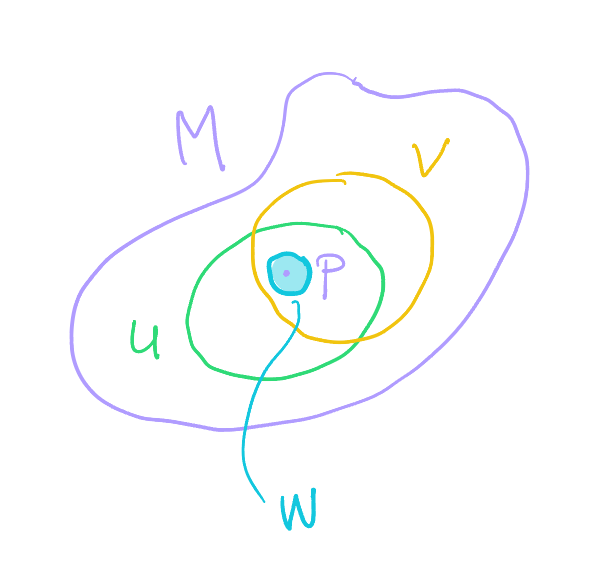
\includegraphics{images/2_3-def_2_3_1.png}
\end{marginfigure}

\begin{exercise}
  Make a drawing to clarify the meaning of this definition.
  Try to define three different functions with the same germ at some point $p$ and with different germs at some other point $p'$.
  Make it concrete: pick $M=\R$ first and then try with $M=\R^3$, and choose some specific values for $p$ and $p'$.
\end{exercise}

Germs define an equivalence relation on the set of smooth functions defined on a neighbourhood of a point $p$: $(U, f) \sim_p (V, g)$ if they have the same germ at $p$. Then, a germ $[f]_p$, where $(U, f)$ is one representative for $[f]_p$, is an equivalence class in the quotient space
\begin{equation}
  C_p^\infty(M) := C^\infty(M)/\!\sim_p.
\end{equation}

\begin{exercise}
  Show that $\sim_p$ defined above is an equivalence relation in $C^\infty(M)$.
\end{exercise}

For $c\in\R$ and $[f]_p, [g]_p$ germs with representatives $(U, f), (V, g)$, we have
\begin{itemize}
  \item $[f]_p + [g]_p$ is the germ with representative $(U\cap V, f+g)$;
  \item $[f]_p [g]_p$ is the germ with representative $(U\cap V, f g)$;
  \item $c[f]_p$ is the germ with representative $(U, cf)$.
\end{itemize}
Therefore, $C_p^\infty(M)$ is also an algebra over $\R$.

\begin{exercise}
  Check that the operations above are well--defined.
\end{exercise}

Germs are the apotheosis of locality: a germ at $p$ has a well--defined value at $p$ and nowhere else.
This results in a map,
\begin{equation}
  \eval_p: C_p^\infty(M) \to \R, \quad
  \eval_p([f]_p) := f(p),
\end{equation}
where $(V,f)$ is any representative of $[f]_p$.
\begin{exercise}
  Check that the $\eval_p$ map is well--defined.
\end{exercise}

We can now go back to our discussion of euclidean derivations to motivate our definition of tangent vectors.

\begin{example}\label{ex:euclideanD}
  Let $U\subset\R^n$ open\footnote{In what follows, we will think of $U$ as both an open subset of $\R^n$ and a smooth manifold depending on what is most convenient for us.} and $f\in C^\infty(U)$.
  For $x\in U$ and $v\in\R^n$ we have seen that $Df(x)$ can be interpreted as a matrix that consumes the vector $v$ to produce a number $Df(x)v$.
  In such interpretation $f$ is fixed and only $x$ and $v$ vary, however there is no reason for this restriction.

  Indeed, an alternative interpretation lets also $f$ vary and considers the action of differentiation as a map
  \begin{equation}
    U \times \R^n \times C^\infty(U) \to \R,\quad
    (x,v,f) \mapsto Df(x) v.
  \end{equation}
  And since we are here changing the cards on the table, let us consider $x$ and $v$ fixed and instead only let $f$ vary:
  \begin{equation}\label{eq:mapxvtoD}
    (x,v):C^\infty(U) \to\R, \quad (x,v)(f) := Df(x)v.
  \end{equation}
  By the definition~\eqref{eq:diff} of the euclidean differential, we know that it is a local concept: the value $Df(x)$ only depends on the value of $f$ in an arbitrarily small neighbourhood of $x$, that is, on the germ of $f$ at $x$.
  Thus we can rephrase~\eqref{eq:mapxvtoD} by saying that $v$ defines a \emph{linear} map
  \begin{equation}
    v : C_x^\infty(U) \to \R, \quad
    v([f]_x) := Df(x) v.
  \end{equation}
  In fact, this is not just a linear map, it also satisfies a \emph{derivation} property, in the sense that
  \begin{equation}
    v([f]_x [g]_x) =
    \eval_x([f]_x)v([g]_x)
    + \eval_x([g]_x)v([f]_x).
  \end{equation}
  Which, rewritten in a more familiar form, is just a way to rewrite the \emph{Leibniz rule}:
  \begin{equation}
    D(fg)(x) v = f(x)\,Dg(x)v + g(x)\,Df(x)v.
  \end{equation}

  Note that we have now \emph{two} different interpretations for $v$: it is both a vector in $\R^n$ and a linear map $C_x^\infty(U) \to \R$ satisfying the derivation property.
\end{example}

Motivated by Example~\ref{ex:euclideanD}, we define a tangent vector as a derivation on the space of germs.

\begin{definition}
  Let $M$ be a smooth manifold of dimension $n$ and let $p\in M$.
  A \emph{tangent vector at $p$} is a linear map
  \marginnote{Keep always in mind that the value $v([f]_p)$ only depends on the value of $f$ around the point $p$.}
  \begin{equation}\label{def:tangentvector}
    v: C_p^\infty(M)\to\R
  \end{equation}
  which is also a derivation, i.e.
  \begin{equation}
    v([f]_p [g]_p) =
    \eval_p([f]_p)v([g]_p)
    + \eval_p([g]_p)v([f]_p).
  \end{equation}

  Since a tangent vector is a linear map from the vector space $C_p^\infty(M)$ to $\R$, the set of all tangent vectors at a point $p$ is itself a vector space\footnote{Exercise: why is this true?} which we denote $T_p M$ and call \emph{tangent space}.
\end{definition}

Let's poke our definition and see if it makes any sense.
Do these vectors at least satisfy the most elementary properties of derivations?
For example, is the derivative of constant functions actually zero?

\begin{lemma}\label{lem:f'0is0forconst}
  Let $M$ be a smooth manifold, let $U\subset M$ be an open set containing $p$ and let $v\in T_p M$.
  Denote by $[c]_p$ the germ of a constant function $(U, p \mapsto c)$.
  Then $v([c]_p) = 0$.
\end{lemma}
\begin{proof}
  Since $[c]_p = c [1]_p$, by linearity we have $v([c]_p) = c v([1]_p)$.
  Thus, it will be enough to show that $v([1]_p) = 0$.
  Since $v$ is a derivation, the algebraic properties of the space of germs imply
  \marginnote{Keep this simple trick in mind, it will be useful in the future.}
  \begin{equation}
    v([1]_p) = v([1]_p [1]_p) = 2 \eval_p([1]_p)v([1]_p) = 2 v([1]_p).
  \end{equation}
  Thus, $v([1]_p) = 0$, concluding the proof.
\end{proof}

As you can see, working with equivalence classes is doable... but it is also unnecessarily cumbersome.
As we did with atlases, we would like to get it over with.

\begin{definition}
  Let $M$ be a smooth manifold and $p\in M$.
  Let $W\subseteq M$ be any neighbourhood of $p$.
  \marginnote{We are still talking about derivations of functions at specific points, not to be confused with the derivations of the algebra $C^\infty(W)$ which we will introduce later and will be maps of the kind $C^\infty(W)\to C^\infty(W)$.}
  A map $w_p:C^\infty(W)\to\R$ is called a \emph{derivation of $C^\infty(W)$ at $p$} if it is linear over $\R$ and satisfies Leibniz rule
  \begin{equation}
    w_p(fg) = f(p)w_p(g) + g(p)w_p(f).
  \end{equation}
\end{definition}

If $v\in T_p M$, then we already saw that $v$ naturally defines a derivation $w_p$ of $C^\infty(W)$ at $p$ for any open neighbourhood $W$ of $p$.
In this case
\begin{equation}\label{eq:derivfromtg}
  w_p(f) := v([f]_p).
\end{equation}
Showing that the opposite is also true will require a bit of work.

\begin{proposition}
  Let $M$ be a smooth manifold, $p\in M$ and $W$ any neighbourhood of $p$.
  Then there is a linear isomorphism between $T_p M$ and the space of derivations of $C^\infty(W)$ at $p$.
\end{proposition}
\begin{proof}
  To prove the theorem we need to invert~\eqref{eq:derivfromtg} and define a tangent vector in terms of of a derivation of $C^\infty(W)$ at $p$.
  We will proceed in three steps.

  \newthought{Step I}. Let $w_p:C^\infty(W) \to\R$ be a derivation at $p$ and suppose that $f\in C^\infty(W)$ is identically zero on a neighbourhood $W_0\subset W$ of $p$.
  We are going to show that $w_p(f)=0$.

  By Proposition~\ref{prop:cutoff}, we can find a cutoff function $\rho:M\to\R$ such that $\rho(p)=1$ in a closed set $W_1 \subset W_0$ and $\supp(\rho) \subset W_0$. Consider now $g = \rho f : W \to \R$.
  Then $g$ is identically zero everywhere in $W$, and thus\footnote{Follows by linearity, exactly as in Lemma~\ref{lem:f'0is0forconst}} $w_p(g) = 0$.
  Using Leibniz rule, the fact that $\rho(p)=1$ and $f(p) = 0$, we get
  \begin{equation}
    0 = w_p(g) = w_p(\rho f) = \rho(p) w_p(f) + f(p)w_p(\rho) = w_p(f).
  \end{equation}

  \newthought{Step II}.
  Let $[f]_p\in C_p^\infty(M)$.
  We want to show that it is always possible to find a representative for $[f]_p$ with domain $W$, that is, there exists $g\in C^\infty(W)$ such that $[g]_p = [f]_p$.
  Let $(V, f)$ be any representative of $[f]_p$.
  Since germs are local, if necessary, we can shrink $V$ so that $V\subset W$.
  Here comes the tricky bit: we need to extend $f$ to a function $g$ defined on $W$ which coincides with $f$ in some neighbourhood of $p$!
  To this end, choose\footnote{We can do this because topological manifolds are locally compact Hausdorff spaces, which implies that every point has a neighbourhood with compact closure. You can take it for granted or have a look at e.g.~\cite[Lemma 4.65]{book:lee:topology} or~\cite{book:munkres:topology}.} a smaller neighbourhood $U$ of $p$ such that $\overline{U}\subset V\subset W$.
  Again, Proposition~\ref{prop:cutoff} comes to the rescue. Apply it with $K=\overline{U}$ and ``$U$'' equal\footnote{Meaning the set that we called $U$ in Proposition~\ref{prop:cutoff} is what we denoted $V$ here.} to $V$, and consider the smooth\footnote{Can you see why it is smooth?} map
  \begin{equation}
    g:W\to\R, \quad
    g(q) := \begin{cases}
      \rho(q)f(q), & q\in V,             \\
      0,           & q \in W\setminus V.
    \end{cases}
  \end{equation}
  Since $g|_U = f$, we have $[g]_p = [f]_p$, proving the claim.

  \newthought{Step III}. We can now complete the proof.
  Let $w_p:C^\infty(W) \to\R$ be a derivation at $p$.
  A tangent vector is a linear map $v:C_p^\infty(M)\to\R$, see~\eqref{def:tangentvector}, and a derivation.
  We would like to define one in terms of $w$.
Given any $[f]_p\in C_p^\infty(W)$, the previous step guarantees that there exists a representative\footnote{Here we have been using $\widetilde{f}$ to emphasize that the specific function may be different from $f$ on the set. Since it makes no difference for any practical purpose, later on we will reuse the same symbol $f$ without further comments.} $(W,\widetilde{f})$ for it, so we can define
  \begin{equation}
    v([f]_p) := w_p(\widetilde{f}), \quad\mbox{where $(W,\widetilde{f})$ is any representative of $[f]_p$}.
  \end{equation}
  Such $v$ is a derivation by construction, so if it is well-defined, we are done.
  To this end, assume that there exists a different representative $(W, g)$ for $[f]_p$.
  Then, by definition, there exists a neighbourhood $V\subset W$ of $p$ such that $\widetilde{f}|_V = g|_V$.
  By linearity, $w_p(\widetilde{f}) - w_p(g) = w_p(\widetilde{f}-g)$ and, by the first step in the proof, $w_p(\widetilde{f}-g) = 0$.

  The assignment $w_p\mapsto v$ inverts~\eqref{eq:derivfromtg}, completing the proof.
\end{proof}

This seemingly innocent proposition, has some very important consequences.

First of all, from now on we are free to interpret tangent vectors in $T_p M$ as derivations of $C^\infty(W)$ at $p$ for \emph{any}\footnote{In particular, it is often convenient to have $W$ coincide with the domain of a chart or with the whole manifold $M$.} open set $W\subseteq M$ containing $p$.
As it turns out, this allows us to give our first example of tangent vector.

\begin{example}\label{ex:partialderivative}
  Let $M$ be a smooth manifold of dimension $n$ and $\varphi: U \to V\subset\R^n$ a chart on $U\subset M$.
  Let $x^i = r^i \circ \varphi$ denote the local coordinates\footnote{See Notation~\ref{ntn:coords}.} of $\varphi$.
  For any $p\in U$, we can define a derivation of $C^\infty(U)$ at $p$ as
  \begin{align}
     & \frac{\partial}{\partial x^i}\Big|_p : C^\infty(U) \to \R,                                                             \\
     & \frac{\partial}{\partial x^i}\Big|_p (f) := \frac{\partial f}{\partial x^i}(p) := D_i(f\circ\varphi^{-1})(\varphi(p)).
  \end{align}
  From now on, it will get more and more convenient to draw commutative diagrams to see ``how things are moving around'':
  \begin{equation}
    \begin{tikzcd}[column sep = huge, row sep = huge]
      M\supset U \arrow[r, "\varphi" description] \arrow[d, "f" description] & V \subset\R^n \arrow [dl, "f\circ\varphi^{-1}" description]\\
      \R &
    \end{tikzcd}
  \end{equation}
  We will soon see that $\left\{\frac{\partial}{\partial x^i}\Big|_p \mid 1\leq i\leq n\right\}$ forms a basis for $T_p M$.
\end{example}

Secondly, we can immediately state some very useful corollaries.

\begin{corollary}\label{cor:tgsubspace}
  Let $M$ be a smooth manifold and let $W\subseteq M$ be a non-empty open set considered as a smooth manifold\footnote{Cf. Exercise~\ref{exe:subsetsmanifolds}.}.
  Then, for any $p\in W$ there is a canonical identification $T_p W \simeq T_p M$.
\end{corollary}

\begin{corollary}\label{cor:derzero}
  Let $M$ be a smooth manifold and $p\in M$.
  Let $W\subseteq M$ be an open neighbourhood of $p$.
  If $f\in C^\infty(W)$ is constant in a neighbourhood of $p$, then $v(f) = 0$ for all $v\in T_p M$.
\end{corollary}

With these new tools at hand, we are ready to state and prove an important result on the size of the tangent spaces.
As it turns out, if $M$ is an $n$-dimensional manifold, $T_pM$ is a finite dimensional vector space of the same dimension $n$, and thus isomorphic to $\R^n$.

\begin{theorem}\label{thm:dimensionTpM}
  Let $M$ be a smooth manifold of dimension $n$ and $p\in M$.
  Then $T_pM$ is a vector space of dimension $n$.
\end{theorem}

The theorem will follow immediately once we construct a basis for $T_pM$.
To that end, we need a preliminary result from multivariable analysis.

\begin{lemma}\label{lem:Taylor}
  Let $U\subset\R^n$, $0\in U$, be a star-shaped\footnote{An open set $U\subset\R^n$ containing the origin, $0\in U$, is called \emph{star-shaped} if $U$ also contains the line segment from $0$ to $x$ for any $x\in U$.} open set and $h\in C^\infty(U)$.
  Then, there exist $n$ smooth functions $g_i: U \to \R$, $1\leq i \leq n$, such that $g_i(0) = D_i h(0)$ and
  \begin{equation}
    h = h(0) + r^i g_i
  \end{equation}
  \marginnote[-2em]{$\leftarrow$ This is our first use of Einstein notation, this equation should be read as $h(x) = h(0) + \sum_{i=1}^n r^i(x) g_i(x)$.
    Using the global euclidean chart, $x^i = r^i(x)$ and $h(x) = h(0) + \sum_{i=1}^n x^i g_i(x)$, which you may recognize as the first iteration of the usual Taylor-MacLaurin formula.}
  where $r^i$ are the coordinates introduced in Notation~\ref{ntn:coords}.
\end{lemma}
\begin{proof}
  Fix a point $x = (x^1, \ldots, x^n) \in U$.
  Let $\gamma_x:[0,1]\to U$ denote the line segment from $0$ to $x$, parametrized as $\gamma_x(t) = tx$.

  By the chain rule,
  \begin{equation}
    \frac{d}{dt}(h \circ \gamma_x) (t) = \left(D_i h(t x)\right) \cdot \frac{d}{dt} (t x^i) = x^i D_i h(t x).
  \end{equation}
  \marginnote[-2.5em]{$\leftarrow$ Again, due to Einstein notation, the right hand side should be read as $\sum_{i=1}^n x^i D_i h(t x)$.}
  The fundamental theorem of calculus then implies
  \begin{align}
    h(x) - h(0) & = (h \circ \gamma_x)(1) - (h \circ \gamma_x)(0)                                 \\
                & = \int_0^1 \frac{d}{dt}(h \circ \gamma_x)(t)\;dt = x^i \int_0^1 D_i h(tx)\; dt.
  \end{align}
  \marginnote[-2.3em]{$\leftarrow$ For one last time, due to Einstein notation, the right hand side should be read as $\sum_{i=1}^n x^i \int_0^1 D_i h(t x)\; dt$.}

  Since $x^i = r^i(x)$ by definition, the theorem follows by defining
  \begin{equation}
    g_i(x) := \int_0^1 D_i h(tx)\; dt.
  \end{equation}
\end{proof}

Theorem~\ref{thm:dimensionTpM} now follows from the next statement.

\begin{proposition}\label{prop:basis_TpM}
  Let $M$ be a smooth manifold of dimension $n$ and $p\in M$.
  Let $\varphi: U \to V$ be a chart on $M$ around $p$, i.e. $p\in U$.
  Then any tangent vector $v\in T_p M$ can be uniquely written as a linear combination
  \begin{equation}
    v = v^i \frac{\partial}{\partial x^i}\Big|_p, \quad v_i = v(x^i).
  \end{equation}
  \marginnote[-3em]{$\leftarrow$ Since we consider upper indices in the denominator as lower indices, the equation should be read as $v = \sum_{i=1}^n v^i \frac{\partial}{\partial x^i}\Big|_p$. If $M=\R^n$, what we are saying here is that $v(f) = v\cdot\nabla f = Df\; v$, that is, $v$ acts as the directional derivative in its direction.}
  Thus, $\left\{\frac{\partial}{\partial x^i}\Big|_p\;\mid\; 1\leq i\leq n\right\}$ is a basis of $T_p M$.
\end{proposition}
\begin{proof}
  We may assume without loss of generality that $\varphi(p) = 0$ and, thanks to Corollary~\ref{cor:tgsubspace}, that $U$ is star-shaped.
  Let $f\in C^\infty(U)$.
  By Lemma~\ref{lem:Taylor} with $h = f \circ \varphi^{-1}$ we get
  \begin{equation}
    f = f(p) + x^i (g_i \circ \varphi),
    \quad g_i(0) = D_i (f \circ \varphi^{-1})(0) = \frac{\partial}{\partial x_i}\Big|_p(f).
  \end{equation}
  \marginnote{If we are careful with the meaning of our notation, we could write more succintly $\frac{\partial f}{\partial x_i}(p)$ in place of $\frac{\partial}{\partial x_i}\big|_p(f)$ in the same fashion as in Example~\ref{ex:partialderivative}.}
  Thus, for any derivation $v$, we obtain
  \begin{equation}
    v(f) = v(f(p)) + v(x^i)g_i(0) + x^i(p) v(g_i\circ\varphi) = v(x^i)  \frac{\partial}{\partial x_i}\Big|_p(f).
  \end{equation}
  The right hand side is obtained observing that $\varphi(p) = 0$, and thus the components $x^i(p) = 0$ are all zero, and applying Corollary~\ref{cor:derzero} to the constant $f(p)$, which implies $v(f(p)) = 0$.

  It follows that the set $\left\{\frac{\partial}{\partial x^i}\Big|_p\;\mid\; 1\leq i\leq n\right\}$ spans $T_p M$.
  We now need to show that its elements are linearly independent.
  Observe that
  \begin{align}
    \frac{\partial}{\partial x_i}\Big|_p (x^j) & =
    \frac{\partial}{\partial x_i}\Big|_p (r^j \circ \varphi)                                               \\
                                               & = D_i (r^j \circ \varphi \circ \varphi^{-1}) (\varphi(p)) \\
                                               & = D_i r^j(\varphi(p)) = \delta^j_i.
  \end{align}
  Thus, if
  \begin{equation}
    v = a^i \frac{\partial}{\partial x_i}\Big|_p = 0,
  \end{equation}
  by letting $v$ act on $x^j$, $1\leq j\leq n$, we obtain $(a^1, \ldots, a^n) = 0$, proving the linear independence.
\end{proof}

\begin{remark}[Change of coordinates]\label{rmk:chg_coords}
  Suppose $\varphi$ and $\psi$ are two different charts about $p$, with corresponding coordinates $x^i := r^i \circ \varphi$ and $y^i := r^i \circ \psi$.
  Taking $v = \frac{\partial}{\partial y^j}\Big|_p$ in the previous proposition implies that
  \begin{equation}
    \frac{\partial}{\partial y^j}\Big|_p =
    \frac{\partial}{\partial y^j}\Big|_p (x^i) \frac{\partial}{\partial x^i}\Big|_p.
  \end{equation}
  \marginnote[-3em]{If we start getting used to thinking of these vectors as actual derivatives and hide the dependence on $p$, then the equation on the left can be rewritten as $\frac{\partial}{\partial y^j} =
      \frac{\partial x^i}{\partial y^j} \frac{\partial}{\partial x^i}$.}
  %
  Expanding the definitions, we get
  \begin{equation}
    \frac{\partial}{\partial y^j}\Big|_p (x^i) =
    D_j(x^i\circ\psi^{-1})(\psi(p)) =
    D_j(r^i \circ \varphi \circ \psi^{-1})(\psi(p)),
  \end{equation}
  which is the $(i,j)$th entry in the matrix $D(\varphi\circ\psi^{-1})(\psi(p))$ as discussed at the beginning of Section~\ref{sec:dd}.
  In other words, $D(\varphi\circ\psi^{-1})(\psi(p))$ is the transition matrix from the basis $\left\{\frac{\partial}{\partial y^i}\Big|_p\;\mid\; 1\leq i\leq n\right\}$ to the basis $\left\{\frac{\partial}{\partial x^i}\Big|_p\;\mid\; 1\leq i\leq n\right\}$.
\end{remark}

\begin{example}
  The transition map between the standard euclidean coordinates and the polar coordinates on appropriate open sets in $\R^2$ is given by $(x,y) = (\rho\cos(\theta), \rho\sin(\theta))$. Let $p\in\R^2$ denote the point with coordinates $(\rho, \theta) = (3, \pi)$ and $v\in T_p\R^2$ the tangent vector with polar coordinate representation
  \begin{equation}
    v = 5\frac{\partial}{\partial \rho}\Big|_p - \frac{\partial}{\partial \theta}\Big|_p.
  \end{equation}
  Applying the equations in Remark~\ref{rmk:chg_coords}, we get
  \begin{align}
    \frac{\partial}{\partial \rho}\Big|_p
     & = \cos(\pi)\frac{\partial}{\partial x}\Big|_p + \sin(\pi)\frac{\partial}{\partial y}\Big|_p = - \frac{\partial}{\partial x}\Big|_p      \\
    \frac{\partial}{\partial \theta}\Big|_p
     & = -3\sin(\pi)\frac{\partial}{\partial x}\Big|_p + 3\cos(\pi)\frac{\partial}{\partial y}\Big|_p = -3 \frac{\partial}{\partial y}\Big|_p,
  \end{align}
  and thus, the vector $v$ in standard coordinates is represented by
  \begin{equation}
    v = - 5 \frac{\partial}{\partial x}\Big|_p + 3 \frac{\partial}{\partial y}\Big|_p.
  \end{equation}
\end{example}

\begin{exercise}
  Let $(x,y)$ denote the standard coordinates on $\R^2$.
  \begin{enumerate}
    \item Show that $(\widetilde{x}, \widetilde{y})$, where
          \begin{equation}
            \widetilde{x} = x
            \quad\mbox{and}\quad
            \widetilde{y} = y + x^3,
          \end{equation}
          are global smooth coordinates in $\R^2$.
    \item Let $p=(1,0)\in\R^2$ in standard coordinates.
          Show that $\frac{\partial}{\partial x}\Big|_p \neq \frac{\partial}{\partial \widetilde x}\Big|_p$ even though the respective coordinate functions are identically equal.
  \end{enumerate}
  This shows that the coordinate vectors in the tangent space depend on the whole coordinate system and not just on the single coordinate function they are associated to.
\end{exercise}

\newthought{We already mentioned} that there are multiple equivalent definitions of the tangent space. In the following exercises you will provide one in terms of charts and euclidean derivatives.
Soon, we will see yet another definition.

\begin{exercise}\label{exe:vsstruct}
  Let $\{V_\alpha \mid \alpha\in A\}$ be a family of vector spaces indexed by a set $A$, let $W$ be a fixed set and let $T_\alpha: V_\alpha\to W$ be a bijection for all $\alpha\in A$.
  Assume that for any $\alpha, \beta \in A$, the composition $T_\beta^{-1}\circ T_\alpha : V_\alpha \to V_\beta$ is a linear isomorphism.
  Show that there is a unique vector space structure on $W$ such that each $T_\alpha$ is a linear isomorphism.
\end{exercise}

\begin{exercise}[Tangent vectors as equivalence classes of charts and vectors]
  Let $M$ be a smooth $m$-manifold with maximal smooth atlas $\cA$.
  For $p\in M$, let $\cA_p \subset \cA$ denote the set of charts $\varphi\in\cA$ such that $p$ lies in the domain of $\varphi$.
  \begin{enumerate}
    \item Show that
          \begin{equation}
            (v,\varphi) \sim (w, \psi)
            \quad\Longleftrightarrow\quad
            D(\psi \circ \varphi^{-1})(\varphi(p))v = w.
          \end{equation}
          defines an equivalence relation on $\R^m\times\cA_p$.
    \item Let $\cT_p$ denote the set of equivalence classes $[(v,\varphi)]\in \R^m\times\cA_p/\!\sim$. For $\varphi\in\cA_p$, show that the map $T_\varphi:\R^m\to\cT_p$ given by $T_\varphi v := [(v,\varphi)]$ is a bijection.
          Deduce\footnote{Hint: use the previous exercise!} that $\cT_p$ admits a unique vector space structure such that each $T_\varphi$ is a linear isomorphism.
    \item Let $\varphi$ be a chart defined on a neighbourhood of $p$ with local coordinates $x^i = r^i \circ \varphi$ and let $\hat T_\varphi :\R^m \to T_pM$ denote\footnote{As it turns out, this is the same as $T_x$ defined in~\eqref{def:lin_iso_Tp}, however in this exercise we use a different notation to emphasize the dependence on the chart.} the linear isomorphism defined by $\hat T_\varphi e_i = \frac{\partial}{\partial x^i}\big|_p$.
          Show that there exists a linear isomorphism $\mathcal{S}_p:\cT_p\to T_pM$ which in addition satisfies $\mathcal{S}_p \circ T_\varphi = \hat T_\varphi$ for every chart $\varphi$ about $p$.
  \end{enumerate}
\end{exercise}

\section{The differential of a smooth map}\label{sec:diffsmooth}

\newthought{In the case of a smooth map between euclidean spaces}, the total derivative of the map at a point (represented by its Jacobian matrix) is a linear map that represents the best linear approximation to the map near the given point.
\marginnote{If you are curious about what happens if you consider higher order approximations, try to look up \emph{Jet Space} with your favourite search engine.}
In the manifold case there is a similar linear map but, as we discussed, it makes no sense to talk about a linear map between manifolds: we need to find a suitable linear map between tangent spaces.

It should not come a surprise that with the constructions developed so far not only do we have one such map, but we can directly relate it to a derivative.

\begin{definition}\label{def:differentialMap}
  Let $F: M \to N$ be a smooth map between the smooth manifolds $M$ and $N$, and let $p\in M$.
  The \emph{differential $d F_p$ of $F$ at $p$} is the map\footnote{In the differential geometry literature, the differential has many names: you can find it called \emph{tangent map}, \emph{total derivative} or \emph{derivative} of $F$.
    Since it ``pushes'' tangent vectors forward from the domain manifold to the codomain, it is also called the \emph{pushforward}. If that was not enough, different authors use different notations for it: besides $dF_p(v)$, you can find $F_* v_p$, $F'(p)$, $T_pF$, $DF(p)[v]$ or variations thereof.}
  \begin{equation}
    d F_p : T_p M \to T_{F(p)} N, \qquad d F_p (v) (f) := v(f\circ F), \quad \forall f\in C^\infty(N).
  \end{equation}
\end{definition}

Indeed, $v \mapsto d F_p (v)$ is a linear map (why?) defining a derivation at $F(p)$ acting on functions in $C^\infty(N)$ (why?) and, as such, is also a tangent vector in $T_{F(p)}N$.

\begin{exercise}
  Answer the two \emph{(why?)} above.
\end{exercise}
\begin{exercise}
  Let $M = \R^3$ and $N = \R^2$ with coordinates $x=(x^1,x^2,x^3)$ and $y=(y^1,y^2)$ respectively.
  Consider the function $F(x^1,x^2,x^3) = (x^1 x^3, (x^2)^2-1)$.
  What is $d F_{(1,1,1)} \left(\frac{\partial}{\partial x^1} - 2 \frac{\partial}{\partial x^2}\right)$?
\end{exercise}

\begin{theorem}[The chain rule on manifolds]\label{thm:chainrule_mfld}
  Let $M, N, P$ be smooth manifolds and $F: M \to N$, $G: N\to P$ be two smooth maps. Then
  \marginnote{The alternative $D$ notation, in this case, makes the relation to the usual chain rule even more evident: $D(G\circ F)(p) = DG(F(p))\circ DF(p)$.}
  \begin{equation}
    d(G\circ F)_p = dG_{F(p)} \circ dF_p.
  \end{equation}
\end{theorem}
\begin{proof}
  Since $dF_p : T_p M \to T_{F(p)}N$ and $dG_{F(p)}: T_{F(p)}N \to T_{G(F(p))}P$, the map $d(G\circ F)_p: T_p M \to T_{G(F(p))}P$ has the right domain and codomain.
  Take now $v\in T_p M$ and $f\in C^\infty(P)$. We get
  \begin{align}
    d(G\circ F)_p(v)(f) & = v(f\circ G \circ F)
    = dF_p (v)(f\circ G)                                                  \\
                        & \stackrel{(\bigstar)}{=} dG_{F(p)}(dF_p (v))(f)
    = dG_{F(p)} \circ dF_p (v)(f),
  \end{align}
  where in $(\bigstar)$ we used the fact that $dF_p (v)\in T_{F(p)}N$.
\end{proof}

\begin{remark}
  The differential of the identity map $\id_M:M\to M$ at any point $p\in M$ is the identity map
  \begin{equation}
    \id_{T_pM}: T_pM \to T_pM.
  \end{equation}
  Indeed, $d (\id_M)_p(v)(f) = v(f\circ\id_M) = v(f)$ for any $v\in T_pM$ and any $f\in C^\infty(M)$.
\end{remark}

The definition we gave seems quite abstract, let's see what it looks like in coordinates.

\begin{proposition}\label{prop:DiffCoords}
  Let $F:M^m\to N^n$ be a smooth map between smooth manifolds.
  Let $p\in M$, and let $\varphi : U \to \varphi(U)$ be a chart on $M$ about $p$ and $\psi: V \to \psi(V)$ be a chart on $N$ about $F(p)$.
  If $(x^i)$ denotes the local coordinates of $\varphi$ and $(y^i)$ the ones of $\psi$, the matrix of $dF_p$ with respect to the bases $\left\{\frac{\partial}{\partial x^j}\big|_p \;\mid\; j=1,\ldots,m\right\}$ of $T_pM$ and $\left\{\frac{\partial}{\partial y^j}\big|_{F(p)} \;\mid\; j=1,\ldots,n\right\}$ of $T_{F(p)}N$ is given by the Jacobian matrix $D(\psi\circ F \circ\varphi^{-1})(\varphi(p))$.
\end{proposition}
\begin{proof}
  The proof follows from the following direct computation after observing that the number $D_j(r^i \circ \psi \circ F \circ \varphi^{-1})(\varphi(p))$ is the $(i,j)$ entry of the Jacobian matrix $D(\psi\circ F \circ\varphi^{-1})(\varphi(p))$. For any $j=1,\ldots,m$, Remark~\ref{rmk:chg_coords} implies
  \begin{align}
    dF_p \left(\frac{\partial}{\partial x^j}\Big|_p\right)
     & =                                                                                                   %\sum_{i=1}^n 
    dF_p \left(\frac{\partial}{\partial x^j}\Big|_p\right) (y^i) \frac{\partial}{\partial y^i}\Big|_{F(p)} \\
     & =                                                                                                   %\sum_{i=1}^n 
    \frac{\partial}{\partial x^j}\Big|_p (y^i \circ F) \frac{\partial}{\partial y^i}\Big|_{F(p)}           \\
     & =                                                                                                   %\sum_{i=1}^n 
    D_j(r^i \circ \psi \circ F \circ \varphi^{-1})(\varphi(p)) \frac{\partial}{\partial y^i}\Big|_{F(p)}.
  \end{align}
\end{proof}

\begin{exercise}
  Show that the matrix of $d F_p$ in terms of the coordinate bases is
  \begin{equation}
    \begin{pmatrix}
      \frac{\partial F^1}{\partial x^1} (p) & \cdot  & \frac{\partial F^1}{\partial x^n} (p) \\
      \vdots                                & \ddots & \vdots                                \\
      \frac{\partial F^m}{\partial x^1} (p) & \cdot  & \frac{\partial F^m}{\partial x^n} (p)
    \end{pmatrix}
  \end{equation}
  without using the Proposition above. Here $\frac{\partial F^i}{\partial x^j} (p) = \frac{\partial}{\partial x^j}\big|_p (F^i)$, where $F^i$ is the $i$th component of $F$ with respect to the chart with coordinates $y^j$.\\
  \textit{\small Hint: show that $d F_p \left(\frac{\partial}{\partial x^i}\big|_p\right) (f) = \left(\frac{\partial F^j}{\partial x^i} (p) \frac{\partial}{\partial y^j}\big|_{F(p)}\right) (f)$.}
\end{exercise}

\newthought{A particularly important consequence} of this theorem is that if we set $M=\R^m$ and $N=\R^n$ our definition coincides with the euclidean notion.
This is easily checked by taking $\varphi = \id_{\R^m}$ and $\psi=\id_{\R^n}$.
Then the coordinates $(x^1,\ldots,x^m)$ are the standard euclidean coordinates for $\R^m$ and the coordinates $(y^1,\ldots,y^n)$ the ones for $\R^n$.

Let $f:U\subset\R^m\to\R^n$ be a smooth function and define the linear isomorphisms
\begin{equation}\label{def:lin_iso_Tp}
  \begin{split}
    &T_x : \R^m \to T_x\R^m,\quad T_x e_i = \frac{\partial}{\partial x^i}\Big|_x\\
    &T_y : \R^n \to T_y\R^n,\quad T_y e_i' = \frac{\partial}{\partial y^i}\Big|_y
  \end{split},
\end{equation}
where $\{e_1,\ldots,e_m\}$ denotes the standard basis of $\R^m$ and $\{e_1',\ldots,e_n'\}$ denotes the standard basis of $\R^n$.

On the one hand, we have the total derivative $Df(x):\R^m\to\R^n$ from multivariable calculus: a linear map, the Jacobian matrix of partial derivatives.
On the other, we have the differential $df_x : T_x \R^m \to T_{f(x)}\R^m$ defined above: also a linear map, related to the Jacobian matrix of partial derivatives by Proposition~\ref{prop:DiffCoords}.
In fact we know more, since Proposition~\ref{prop:DiffCoords} tells us that the following diagram commutes:
\begin{equation}
  \begin{tikzcd}[row sep=huge, column sep=huge]
    \R^m \arrow[r, "Df(x)"] \arrow[d, "T_x"]
    & \R^n \arrow[d, "T_{f(x)}"] \\
    T_x\R^m \arrow[r, "df_x"]
    & T_{f(x)}\R^n
  \end{tikzcd}.
\end{equation}

More generally, the same kind of reasoning shows the following fact. For any smooth map $F:M^m \to N^n$ between smooth manifolds, if $\varphi$ is a chart about $x\in M$ with coordinates $(x^i)$ and $\psi$ is a chart about $y=F(x)\in N$ with coordinates $(y^i)$, the following diagram commutes:
\marginnote{Recall that the following commutes: \begin{equation}
    \begin{tikzcd}[row sep=huge, column sep=huge, ampersand replacement=\&]
      M \arrow[r, "F"] \arrow[d, "\varphi"] \& N \arrow[d, "\psi"]\\
      \R^m \arrow[r, "\psi \circ F \circ \varphi^{-1}"]
      \& \R^n
    \end{tikzcd}.
  \end{equation}}
\begin{equation}
  \begin{tikzcd}[row sep=huge, column sep=huge]
    \R^m \arrow[r, "D(\psi \circ F \circ \varphi^{-1})(\varphi(x))"] \arrow[d, "T_x"]
    & \R^n \arrow[d, "T_{F(x)}"] \\
    T_xM \arrow[r, "dF_x"]
    & T_{F(x)}N
  \end{tikzcd},
\end{equation}
where $T_x$ and $T_{F(x)}$ are defined as above.

\newthought{An aspect of the construction above is particularly disturbing}: it forced us to fix a basis on the spaces; if this were truly necessary it would defeat the purpose of this whole chapter.
Fortunately for us, the following exercise shows that, at any given point, the tangent space to a vector space is \emph{canonically}\footnote{That is, independently of the choice of basis.} identified with the vector space itself.

\begin{exercise}\label{ex:tg_curve_iso}
  Let $V$ and $W$ be finite-dimensional vector spaces, endowed with their standard smooth structure (see Exercise~\ref{exe:subsetsmanifolds}).
  \begin{enumerate}
    \item Fix $a\in V$. For any vector $v\in V$ define a map $\cT_a(v) : C^\infty(V) \to \R$ by
          \begin{equation}
            \cT_a(v) f = \frac{d}{dt}\Big|_{t=0} f(a + tv).
          \end{equation}
          Show that the map $v\mapsto \cT_a(v) : V \to T_aV$ is an isomorphism of vector spaces.
    \item Let $L:V\to W$ be a linear map. Show for any $a\in V$ that the following diagram commutes:
          \begin{equation}
            \begin{tikzcd}[row sep=huge, column sep=huge]
              V \arrow[r, "L"] \arrow[d, "\cT_a"]
              & W \arrow[d, "\cT_{La}"] \\
              T_aV \arrow[r, "dL_a"]
              & T_{La}W
            \end{tikzcd}.
          \end{equation}
  \end{enumerate}
\end{exercise}

An important consequence of what we have seen so far is that we can routinely \emph{identify} tangent vectors to a finite-dimensional vector space with elements of the space itself.
More generally, if $M$ is an open submanifold of a vector space $V$, we can combine the identifications $T_p M \simeq T_p V \simeq V$ to obtain a canonical identification of each tangent space to $M$ with $V$.
For example, since $GL_n(\R)$ is an open submanifold of the vector space $\mathrm{Mat}(n, \R)$, we can identify its tangent space at each point $X\in GL_n(\R)$ with the full space of matrices $\mathrm{Mat}(n, \R)$.

\begin{exercise}[Tangent space of a product manifold]
  Let $M_1, \ldots, M_k$ be smooth manifolds (without boundary\footnote{The statement is true also if one (only one!) of the $M_i$ spaces is a smooth manifold with boundary. If there is more than one manifold with boundary, the product space will have ``corners'' that cannot be mapped to half spaces and thus is not a smooth manifold, as a simple example you can consider the closed square $[0,1]\times [0,1]$.}), and for each $j$ let $\pi_j:M_1\times\cdots\times M_k \to M_j$ be the projection onto the $M_j$ factor.
  For any point $p=(p_1,\ldots,p_k)\in M_1\times\cdots\times M_k$, the map
  \begin{align}
    \sigma & : T_p(M_1\times\cdots\times M_k) \to T_p M_1\times\cdots\times T_p M_k \\
    \sigma & : v \mapsto \left(d(\pi_1)_p(v), \ldots, d(\pi_k)_p(v)\right)
  \end{align}
  is an isomorphism.
\end{exercise}

\begin{remark}
  When $M$ is a smooth manifold with boundary and $p$ is an interior point, all the discussions above apply verbatim. In particular, the tangent space at a boundary point of an $n$-dimensional manifold with boundary is also an $n$-dimensional real vector space that can be identified (non-uniquely) with $\R^n$ using a chart containing that point.

  For $p\in\partial M$ the only change that needs to be made is to substitute $\cH^n$ for $\R^n$, with the understanding that the notation $\frac{\partial}{\partial x^i}\big|_{\varphi(p)}$ can be used interchangeably to denote either an element of $T_{\varphi(p)}\R^n$ or of $T_{\varphi(p)}\cH^n$. In the latter case, the $n$th coordinate vector $\frac{\partial}{\partial x^n}\big|_{p}$ should be interpreted as a one-sided derivative.
\end{remark}

In the next section we will give yet another alternative way of defining tangent vectors: less elegant but easier to compute.


\section{Tangent vectors as tangents to curves}

\begin{marginfigure}[1em]
  \includegraphics{2_2-curve-on-M.pdf}
\end{marginfigure}

Exercise~\ref{ex:tg_curve_iso} may have left some thoughts hanging in the air...
From the look of it, it seems that there is a relation between tangent spaces and the velocity of a body moving with constant speed.
In this section we will further explore these thoughts.

\begin{definition}
  If $M$ is a manifold with or without boundary, we define a \emph{(parametrized) curve in M} to be a smooth\footnote{Continuously differentiable would be enough, but assuming it smooth simplifies the exposition.} map $\gamma : I \to M$, where $I=(a,b)\subseteq\R$ is an interval.
  \marginnote{Conventionally, $b=-a=\epsilon>0$ (the reason will be clear in a second) and we denote the coordinate on $\R$ by $t$ and the derivative of $\gamma$ at a point $t$ by $\gamma'(t)$. We say that a curve \emph{starts at $p\in M$} if $0\in I$ and $\gamma(0) = p$.}
\end{definition}

Fix $t\in(a,b)$.
A priori we have two different ways to define the \emph{velocity vector of $\gamma$ at a time $t$}, that is, an element $\gamma'(t) \in T_{\gamma(t)}M$:
\begin{enumerate}[(i)]
  \item We can define a derivation of $C^\infty(M)$ at $\gamma(t)$ by setting
        \begin{equation}\label{eq:tg_curve_der}
          \gamma'(t) (f) := (f\circ\gamma)'(t), \quad f\in C^\infty(M).
        \end{equation}
        \begin{exercise}
          Show that this is indeed a derivation of $C^\infty(M)$ at $\gamma(t)$.
        \end{exercise}
  \item If we think of $\gamma$ as a smooth map between manifolds, we can define the tangent vector via the differential $d\gamma_t$:
        \begin{equation}\label{eq:tg_curve_diff}
          \gamma'(t):= d\gamma_t\left(\frac{\partial}{\partial t}\Big|_t\right) \in T_{\gamma(t)}M.
        \end{equation}
\end{enumerate}

Do these definitions agree?
One way to check is to pick a chart $\varphi: U \to \varphi(U)$ in a neighbourhood of $\gamma(t)$, and compare the expressions in local coordinates. Let $(x^i)$ denote the coordinates of $\varphi$ and define the curves $\gamma^i := x^i \circ \gamma : I\to\R$.
Let's focus on~\eqref{eq:tg_curve_der}. By definition, $\gamma'(t)(x^i) = (x^i\circ\gamma)'(t) = (\gamma^i)'(t)$, therefore by Proposition~\ref{prop:basis_TpM} we get
\begin{equation}\label{eq:tg_curve_vec}
  \gamma'(t) = %\sum_{i=1}^m
  \gamma'(t)(x^i) \frac{\partial}{\partial x^i}\Big|_{\gamma(t)}.
\end{equation}
\begin{exercise}
  Show that applying Proposition~\ref{prop:DiffCoords} to~\eqref{eq:tg_curve_diff} leads to the same formula as~\eqref{eq:tg_curve_vec}.
\end{exercise}

\begin{figure*}[htp]
  \centering
  \includegraphics{2_5-v_cur_full.pdf}
  \caption{The velocity of a curve}
  \label{fig:2_5-v_cur_full}
\end{figure*}

But how can this mapping between curves and tangent vector be well--defined?
Surely, there must be multiple curves with the same velocity at a point which differ outside a neighbourhood of the point.

\begin{lemma}\label{lem:equiv_tg_curves}
  Let $M$ be a smooth manifold and $\gamma, \delta : (-\epsilon, \epsilon) \to M$ two smooth curves with $\gamma(0) = \delta(0)$. Then, $\gamma'(0) = \delta'(0)$ as elements of $T_{\gamma(0)}M$ if and only if for some (and thus any) chart $\varphi:U\to\varphi(U)$, $\gamma(0)\in U$, we have $(\varphi\circ \gamma)'(0) = (\varphi\circ\delta)'(0)$.
\end{lemma}
\begin{proof}
  Let $(x^i)$ denote the coordinates of $\varphi$. The condition $(\varphi\circ \gamma)'(0) = (\varphi\circ\delta)'(0)$ is equivalent as stating that $(\gamma^i)'(0) = (\delta^i)'(0)$, where $\gamma^i = x^i\circ\gamma$ and $\delta^i=x^i\circ\delta$. Then, the claim follows from~\eqref{eq:tg_curve_vec} and the fact that $\left\{\frac{\partial}{\partial x^i}\big|_{\gamma(0)}\right\}$ is a basis of $T_{\gamma(0)}M$.
\end{proof}

This seems to follow a pattern: until now, all the definitions of tangent vectors were in terms of classes of equivalence.
And it would seem reasonable to identify curves that have the same tangent vector at $0$.
There is still a potential problem, though: we don't yet know if \emph{every} tangent vector can be written as the velocity vector of a curve.

\begin{theorem}
  Let $M$ be a smooth $n$-manifold, let $p\in M$ and let $v\in T_pM$.
  There exists a smooth curve $\gamma: (-\epsilon,\epsilon) \to M$ such that $\gamma(0)=p$ and $\gamma'(0) = v$.
\end{theorem}
\begin{proof}
  Let $\varphi:U\to\varphi(U)$ be a chart about $p$ such that $\varphi(p)=0$.
  Let $(x^i)$ denote the coordinates of $\varphi$, as usual, and assume that
  \begin{equation}
    v = a^i \frac{\partial}{\partial x^i}\Big|_p, \qquad a^i \in\R \mbox{ for all } i=1,\ldots,n.
  \end{equation}
  For $\epsilon$ small enough, by continuity the vector $(ta^1, \ldots, ta^n) \in \varphi(U)$ for all $|t|<\epsilon$. Therefore, the curve
  \begin{equation}
    \gamma: (-\epsilon, \epsilon) \to M, \quad \gamma(t):=\varphi^{-1}(ta^1, \ldots, ta^n),
  \end{equation}
  is well-defined, smooth, satisfies $\gamma(0) = p$ and, by~\eqref{eq:tg_curve_vec}, $\gamma'(0) = v$.
\end{proof}

\begin{marginfigure}
  \includegraphics{2_4-v_cur.pdf}
  \caption{With this definition, the coordinate tangent vectors $\partial_{x^i}\in T_p M$ become the tangent vectors defined by the curve \[t \mapsto \varphi^{-1}(x^1(p), \ldots, {x^i(p) + t}, \ldots, x^n(p)).\]}
  \label{fig:2_4-v_cur}
\end{marginfigure}
This means that we can actually give an alternative definition of $T_pM$ in terms of tangents to curves:
\begin{definition}\label{def:tg:ascurvespeed}
  A tangent vector at $p\in M$ is an equivalence class\footnote{Usually we say that two such equivalent curves have \emph{a first order contact at $p$}.} of smooth curves $\gamma:(-\epsilon, \epsilon)\to M$ such that $\gamma(0)=p$, where $\gamma\sim\delta$ if and only if $(\varphi\circ \gamma)'(0) = (\varphi\circ\delta)'(0)$ for some chart $\varphi$ centred about $p$ (see Lemma~\ref{lem:equiv_tg_curves}).
\end{definition}

In fact, it is possible to start the whole tangent space discussion with the above definition. In that case, you would first need to prove Exercise~\ref{exe:vsstruct} and endow $T_pM$ with a vector space structure\footnote{To get the analogue result as Proposition~\ref{prop:basis_TpM}}.

\begin{exercise}
  Show that $T_p M$ defined as the space of tangent vectors at $p$ from Definition~\ref{def:tg:ascurvespeed} has a natural structure of vector space.
\end{exercise}

To conclude this part, the next proposition shows that velocity vectors behave well under composition with smooth maps and give us a direct, explicit and effective way to compute differentials.

\begin{proposition}\label{prop:curves_deriv}
  Let $F:M\to N$ be a smooth map between smooth manifolds and $\gamma:I\to M$ a smooth curve in $M$.
  Then
  \begin{equation}
    d F_{\gamma(t)} (\gamma'(t)) = (F\circ\gamma)'(t).
  \end{equation}
\end{proposition}
\begin{proof}
  We are going to use~\eqref{eq:tg_curve_diff} as definition of $\gamma'(t)$.
  Applying the chain rule we obtain:
  \begin{align}
    d F_{\gamma(t)} (\gamma'(t))
     & = d F_{\gamma(t)} \circ d\gamma_t\left(\frac{\partial}{\partial t}\Big|_t\right) \\
     & = d (F\circ\gamma)_t \left(\frac{\partial}{\partial t}\Big|_t\right)             \\
     & = (F\circ\gamma)'(t).
  \end{align}
\end{proof}

\begin{exercise}
  Give an alternative proof of Proposition~\ref{prop:curves_deriv} using~\eqref{eq:tg_curve_der} as definition for $\gamma'(t)$.\\
  \textit{\small Hint: use the definitions to rewrite the formula in different ways.}
\end{exercise}

\section{The tangent bundle}\label{sec:tangentbundle}

Instead of working separately with the various tangent spaces, we can ``glue'' them together into a big manifold.

\begin{marginfigure}
  \includegraphics{2_6-tg_bdl_proj.pdf}
\end{marginfigure}
\begin{definition}
  The \emph{tangent bundle} $TM$ of $M$ is the disjoint union of the tangent spaces
  \begin{equation}
    TM := \bigsqcup_{p\in M}\left(\{p\}\times T_pM\right)
    = \{(p,v) \;\mid\; p\in M,\, v\in T_pM\}.
  \end{equation}
\end{definition}

Elements in $TM$ are pairs\footnote{We will often abuse notation and identify $T_pM$ with with its image under the canonical injection $v\mapsto(p,v)$ and use interchangeably any of the notations $v$, $v_p$ or $(p,v)$ for a vector in $T_pM$ (depending on how much emphasis we need to put on the base point).} $(p,v)$ of a \emph{base point} $p\in M$ and a \emph{tangent vector} $v\in T_pM$.

To the tangent bundle we associate a surjective map $\pi:TM \to M$, the \emph{projection (onto the base)}, which sends each vector in a tangent space to the point at which it is tangent, that is, $\pi(p,v) = p$.
The second component of the pre-image $\pi^{-1}(\{p\}) = \{p\}\times T_pM$, that is $T_pM$ itself, is called the \emph{fibre} over $p\in M$.
We will come back to this later on once we talk about vector bundles.

\begin{example}
  Let $M\subset \R^n$ be an an open set.
  We can identify $TM$ in a natural way with $M\times\R^n$.
  Since $M\times\R^n \subset \R^{2n}$ and thus is a manifold, we can equip the tangent bundle $TM$ with the structure of a manifold induced by this identification.
\end{example}

As it turns out, this is a particular instance of a more general fact.

\begin{theorem}\label{thm:tgbdlsmoothmfld}
  Let $M$ be a smooth $n$-manifold.
  The smooth structure on $M$ naturally\footnote{In the sense that its definition does not require to make any arbitrary choices.} induces a smooth structure on $TM$, making $TM$ into a smooth manifold of dimension $2n$.
  Moreover, the map $\pi: TM \to M$ is smooth.
\end{theorem}
\begin{proof}
  \marginnote[1em]{In this proof you can see instances of a typical abuse of notation: in the expressions $\widetilde x^i(x)$ we think of the $\widetilde x^i$ as coordinate functions but we think of the $x$ as representing a point in $\varphi(U\cap V)$.}
  \newthought{Step 1: extending charts from $M$ to $TM$.}
  Given a chart $(U,\varphi)$ about $p\in M$, the preimage $\pi^{-1}(U) \subset TM$ is the set of all tangent vectors to $M$ at points of $U$.
  If $(x^i)$ denotes the coordinate functions of $\varphi$, we can define a map $\widetilde\varphi : \pi^{-1}(U) \to \varphi(U)\times\R^n \subset \R^{2n}$ by
  \marginnote{Keep in mind that \begin{equation}\nonumber
      \pi^{-1}(U)= TU = \bigsqcup T_p U \subset \bigsqcup T_p M=TM.
    \end{equation}}
  \begin{align}\label{eq:nat_coords}
    \widetilde\varphi\left(v^i \frac{\partial}{\partial x^i}\Big|_p\right) := \left(x^1(p), \ldots, x^n(p), v^1, \ldots, v^n\right).
  \end{align}
  Since $\widetilde\varphi$ can be explicitly inverted as $\widetilde\varphi^{-1}\left(x^1, \ldots, x^n, v^1, \ldots, v^n\right) = v^i \frac{\partial}{\partial x^i}\Big|_{\varphi^{-1}(x)}$, it defines a bijection onto its image.

  \newthought{Step 2: compatibility of the extended charts.}
  Suppose we have two smooth charts $(U,\varphi)$, $(V,\psi)$ for $M$ with the respective local coordinates $(x^i)$ and $(y^i)$.
  Let $(\pi^{-1}(U),\widetilde\varphi)$, $(\pi^{-1}(V),\widetilde\psi)$ be their extension\footnote{These are called \emph{bundle charts}.} to $TM$ as in the previous step.
  By construction\footnote{They are both homeomorphisms.}, both $\widetilde\varphi(\pi^{-1}(U)\cap\pi^{-1}(V)) = \varphi(U\cap V)\times\R^n$ and $\widetilde\psi(\pi^{-1}(U)\cap\pi^{-1}(V)) = \psi(U\cap V)\times\R^n$ are open in $\R^{2n}$.
  Moreover, we can take advantage of Remark~\ref{rmk:chg_coords} to write explicitly the transition map  $\widetilde\psi\circ\widetilde\varphi^{-1}: \varphi(U\cap V)\times\R^n \to \psi(U\cap V)\times\R^n$ as
  \begin{align}
    \widetilde\psi\circ & \widetilde\varphi^{-1}\left(x^1, \ldots, x^n, v^1, \ldots, v^n\right)                                                            \\
                        & =\left(y^1(p),\ldots, y^n(p), \frac{\partial y^1}{\partial x^j}(p) v^j, \ldots, \frac{\partial y^n}{\partial x^j}(p) v^j\right),
  \end{align}
  where $p = \phi^{-1}(x)$, which is clearly smooth.

  \begin{figure*}[htp]
    \includegraphics{2_7-tg_bdl_coord.pdf}
    \caption{Coordinates for the tangent bundle}
  \end{figure*}

  \newthought{Step 3: $TM$ is a manifold.}
  With the procedure delineated above, a countable smooth atlas $\{(U_i, \varphi_i)\}$ of $M$ induces a countable atlas $\{(\pi^{-1}(U_i), \widetilde\varphi_i)\}$ of $TM$.
  First of all, $\{(\pi^{-1}(U_i)\}$ provides a countable covering of $TM$.
  We need to show that the topology induced by those charts\footnote{Given a family of functions $\cF$ from the same set $X$ into (possibly different) topological spaces, the topology $\cT_{\cF}$ induced by the functions in $\cF$ is the smallest topology such that all the functions are continuous. It is possible to show that such a topology exists and it has as a basis the set $\{V\subset X \,\mid\, \exists n\in\N, f_i\in\cF, U_i \mbox{ open} : \bigcap_{i=1}^n f_i^{-1}(U_i) \}$.} is Hausdorff and second countable.

  Let $(p_1, v_1), (p_2, v_2) \in TM$ be different points: either $p_1\neq p_2$, or $p_1 = p_2$ and $v_1 \neq v_2$.
  \begin{itemize}
    \item In the first case, there are disjoint open sets $V_1, V_2 \subset U_i$ (for some $i$) containing respectively $p_1$ and $p_2$.
          Then $\widetilde\varphi_i^{-1}(\varphi_i(V_1)\times\R^n)$ and $\widetilde\varphi_i^{-1}(\varphi_i(V_2)\times\R^n)$ are disjoint open sets containing respectively $(p_1, v_1)$ and $(p_2, v_2)$.
    \item In the second case, $p=p_1=p_2$ but there are disjoint open sets $V_1,V_2\subset \R^n$ containing $v_1$ and $v_2$ respectively;
          again, the preimages $\widetilde\varphi_i^{-1}(\varphi_i(U_i)\times V_1)$ and $\widetilde\varphi_i^{-1}(\varphi_i(U_2)\times V_2)$ (for some $i$ such that $p\in U_i$) are disjoint open sets containing respectively $(p_1, v_1)$ and $(p_2, v_2)$.
  \end{itemize}

  The countable basis $\{U_j\}$ is a countable basis for the topology of $M$ (which is second countable), taking a countable basis $\{W_k\}$ for the topology of $\R^n$, we can define a countable basis for $TM$ as $\{\widetilde\varphi^{-1}((U_i\cap U_j)\times W_k)\}$.
  The charts defined above make $TM$ automatically euclidean of dimension $2n$.

  \begin{exercise}
    This part of the proof seems unnecessarily detailed.
    Can you simplify it using Lemma~\ref{lem:manifold_chart}?
  \end{exercise}

  \newthought{Step 4: $\pi$ is smooth.} With respect to the charts $(U,\varphi)$ for $M$ and $(\pi^{-1}(U), \widetilde\varphi)$ for $TM$, the coordinate representation of $\pi$ is $\pi(x,v) = x$.
\end{proof}

The coordinates $(x^i, v^i)$ defined by~\eqref{eq:nat_coords} are called \emph{natural (or canonical) coordinates}.

\begin{exercise}
  Let $f:M\to N$ be a smooth map between smooth manifolds.
  Show that its differential $df: TM \to TN$ is a smooth map between smooth manifolds (the respective tangent bundles).\\
  \textit{\small Hint: use the natural differentiable structure on the tangent bundle described above and the definition of smooth map.}
\end{exercise}

\begin{remark}
  In classical mechanics, the configuration space is usually a manifold $M$.
  The tangent bundle $TM$ corresponds to the state space, that is, the space of configurations and velocities. In symbols $x=(q,v)$ is a pair of a configuration $q = \pi(x)$ and a velocity $v\in T_q M$.
  The equations of motion of mechanical systems are often prescribed via a function $L\in C^\infty(TM)$ called Lagrangian of the system.
\end{remark}


\chapter{Submanifolds}\label{ch:sub}
With differentials of smooth functions at hand, we are ready to discuss submanifolds: smaller manifolds sitting inside larger ones.
We have already seen an example at the beginning of the course.
In Exercise~\ref{exe:subsetsmanifolds}, we proved that any open subset $U\subseteq M$ can be made into a smooth manifold with a differentiable structure induced by the one of $M$.
These, somehow trivial, submanifolds are called \emph{open submanifolds}.
But there are many other examples beyond these ones.
In fact, you may have already seen them in multivariable analysis.

In this chapter we will briefly explore what subsets of manifolds are still manifolds of their own rights, how their topologies are related and how their smooth structures are related.
We will conclude the chapter answering the question opened at the beginning of the previous chapter: do tangent spaces really coincide with the intuitive understanding of a tangent hyperplane to a point on the manifold?

\section{Inverse function theorem}

Before getting at the core of the discussion, it is useful to
recall some results from multivariable analysis.

A function $f:\R^m \to \R^n$ between Euclidean spaces has rank $k$ at $x\in\R^m$ if its ($n\times m$) Jacobian matrix $Df(x)$ has rank $k$.
The function has \emph{maximal rank}\footnote{Alternatively, it is of \emph{full rank}.} at $x$ if $k = \min(n,m)$.
When $n=m$, $f$ has maximal rank at $x$ if and only if the square matrix $Df(x)$ is an invertible matrix.

As for many local properties, this definition carries over to manifolds rather ``smoothly''.
%
\begin{definition}
	A smooth map $F:M\to N$ has \emph{rank $k$} at a point $p$ if its differential $dF_p$ has rank $k$, that is, if the linear subspace $dF_p(T_pM)$ has dimension $k$ inside $T_{F(p)}N$.
\end{definition}
%
The same applies to the inverse function theorem:
compare the following statements.
%
\begin{theorem}[Inverse function theorem for $\R^n$]\label{thm:ift}
	Let $U\subset\R^n$ open and $f:U \to \R^n$ be a smooth map.
	Assume that $f$ has maximal rank at some $x\in U$, then there exists an open neighbourhood $\Omega\subset U$ of $x$ such that  $f\big|_\Omega : \Omega \to f(\Omega)$ is a diffeomorphism.
\end{theorem}

\begin{theorem}[Inverse function theorem for manifolds]\label{thm:iftm}
	Let $F:M\to N$ be a smooth function between smooth manifolds without boundary of the same dimension $n$.
	Let $p\in M$ such that $F$ has maximal rank $n$ at $p$.
	Then there exists an open neighbourhood $V$ of $p$ such that the restriction $F|_V : V\to F(V)$ is a diffeomorphism.
\end{theorem}
% \begin{proof}
%   This is a purely local statement.
%   Let $(U,\varphi)$ be a chart about $p\in M$ and let $(V, \psi)$ be a chart about $F(p)\in N$.
%   Since both $\varphi$ and $\psi$ are diffeomorphisms (and thus have maximal rank), the derivative of
%   \begin{equation}
%     \psi \circ F \circ \varphi^{-1}: \varphi(U\cap F^{-1}(V)) \to \psi(F(U)\cap V)
%   \end{equation}
%   has rank $n$ at $\varphi(p)$.
%   Thus the inverse function theorem, Theorem~\ref{thm:ift}, there exists $\Omega \subset \varphi(U\cap F^{-1}(V))$ such that $\psi \circ F \circ \varphi^{-1}\big|_{\Omega}$ is a diffeomorphism.
%   Therefore, once again since both $\varphi$ and $\psi$ are diffeomorphisms, $F\big|_W : W \to F(W)$ is also a diffeomorphism for $W := \varphi^{-1}(\Omega)$.
% \end{proof}
\begin{exercise}
	Use the Euclidean inverse function theorem (Theorem~\ref{thm:ift}) on $\R^n$ to prove Theorem~\ref{thm:iftm}.
\end{exercise}

Note that this theorem can fail for manifold with boundary.
A counterexample\footnote{Exercise: why?} is given by the inclusion map $\cH^n \hookrightarrow \R^n$.

An important observation at this point is that the rank of the mapping
is a crucial property in the inverse function theorem and it is really a
property of its differential.
If we map our manifold via some function $F$ or via its charts into a
Euclidean space in such a way that the rank of the mapping remains fixed,
and thus all the tangent spaces will be mapped to Euclidean spaces of same dimensions,
we may be able to use the shape of the mapping itself to describe the
shape of the manifold.

In fact, if we restrict our attention to constant rank maps, that is,
maps whose rank is the same at all points on the manifold, we can go quite a
long way and show that any manifold locally looks like a projection or an inclusion.
The tool to get there is the following, we will see more clearly the link with
projections and inclusions in the next subsection.

\begin{theorem}[Rank theorem]\label{thm:rank}
	Let $F : M^m \to N^n$ be a smooth function between smooth manifolds without boundary\footnote{The theorem can be extended to allow $M$ with boundary and $N$ without boundary assuming $\ker dF_p \not\subseteq T_p\partial M$ but we will omit this case here to keep the discussion more contained and avoid unnecessary technicalities.}.
	Assume that $F$ is of rank $k$ at all points $p\in M$.
	Then, for all $p\in M$ there exist smooth charts $(U, \varphi)$ centred at $p$ and $(V, \psi)$ centred at $F(p)$ with $F(U)\subseteq V$, such that the coordinate representation of $F$ with respect to the charts $\varphi$ and $\psi$ has the form
	\begin{align}
		\psi \circ F \circ \varphi^{-1} : \varphi(U) \subseteq \R^m & \to \psi(F(U)) \subseteq \R^n                                     \\
		(x^1, \ldots, x^k, x^{k+1}, \ldots, x^m)                    & \mapsto (x^1, \ldots, x^k, \LaTeXunderbrace{0, \ldots, 0}_{n-k}).
	\end{align}
\end{theorem}

We will present here an adaptation of the general proof from \cite[Theorem 4.12]{book:lee}.
If some detail seems unclear, I would recommend you to go through the proof step by step by setting $n=m=2$ and $k=1$, and writing everything down explicitly.

\begin{proof}
	We start with two important observations.

	\newthought{First}. The statement is local on charts: without loss of generality,
	we can fix local coordinates on $M$ and $N$ respectively centred around $p$ and $F(p)$
	and replace them altogether by two open subsets $U\subseteq \R^m$ and $V \subseteq \R^n$.
	So, from now on, $F: U \subseteq \R^m \to V \subseteq \R^n$, $p=(0,\ldots,0)$
	and $F(p) = F(0,\ldots,0) = (0,\ldots,0)$.

	\newthought{Second}. The fact that $F$, and thus $dF$, is of rank $k$, translates to
	the Euclidean setting to the fact that the matrix $DF$ is a $m\times n$ matrix of rank $k$
	and thus with an invertible $k\times k$ submatrix.
	Rearranging the coordinates we can assume, again without loss of generality, that this
	$k\times k$ minor is is the upper left block of the matrix $DF$, that is, the block
	$\left( \frac{\partial F^i}{\partial x^j} \right)$, $i,j = 1,\ldots, k$.

	In what follows, we will denote the coordinates as follows:
	$(x,y) = (x^1, \ldots, x^k, y^1, \ldots, y^{m-k})\in\R^m$
	and $(u,v) = (u^1, \ldots, u^k, v^1, \ldots, v^{n-k})\in\R^n$.
	\medskip

	\newthought{Right hand side}.
	Writing $F(x,y) = (Q(x,y), R(x,y))$ for some smooth maps $Q: U \to \R^k$ and $R: U \to \R^{n-k}$,
	our choice of coordinates after the above observations implies that the gradient of $Q$ with respect to $x$ is regular, that is,
	$\det \left( \frac{\partial Q^i}{\partial x^j} \right) \neq 0$ at $(x,y) = (0,0)$.

	In particular, this implies that we can extend the mapping with
	the identity on the rest of the coordinates to obtain a regular map
	on the whole neighbourhood.
	Let $\varphi : U \to \R^m$ be defined by $\varphi(x,y) = (Q(x,y), y)$. Then,
	\begin{equation}
		D\varphi(0,0) =
		\begin{pmatrix}
			\frac{\partial Q^i}{\partial x^j}(0,0) & \frac{\partial Q^i}{\partial y^j}(0,0) \\
			0                                      & \id_{\R^{m-k}}
		\end{pmatrix}
	\end{equation}
	has nonvanishing determinant by hypothesis.
	The Inverse Function Theorem then implies that there are open neighborhoods $U_0$ of $(0,0)$
	and $W_0$ of $\varphi(0,0)$ such that $\varphi : U_0 \to W_0$ is a diffeomorphism.
	Up to shrinking both domains appropriately, we will assume that $W_0$ is an open cube.

	Denoting $\varphi^{-1}(x,y) = (A(x,y), B(x,y))$ for some smooth functions
	$A : W_0 \to \R^k$ and $B : W_0 \to \R^{m-k}$, we get
	\begin{equation}
		(x,y) = \varphi(A(x,y), B(x,y)) = (Q(A(x,y), B(x,y)), B(x,y)).
	\end{equation}
	That is, $B(x,y) = y$ and therefore $\varphi^{-1}(x,y) = (A(x,y), y)$.
	Moreover, $\varphi \circ \varphi^{-1} = \id$ and thus $Q(A(x,y),y) = x$.

	This leaves us with
	\begin{equation}
		F\circ\varphi^{-1}(x,y) = (x, \widetilde{R}(x,y)),
	\end{equation}
	where $\widetilde{R} : W_0 \to\R^{m-k}$ is defined by $\widetilde{R}(x,y) = R(A(x,y), y)$.
	Therefore, for $(x,y)\in W_0$ we have
	\begin{equation}\label{eq:diff_DFp-1}
		D(F\circ\varphi^{-1})(x,y) = \begin{pmatrix}
			\id_{\R^k}                                        & 0                                                 \\
			\frac{\partial\widetilde{R}^i}{\partial x^j}(x,y) & \frac{\partial\widetilde{R}^i}{\partial y^j}(x,y)
		\end{pmatrix}.
	\end{equation}
	The composition with a diffeomorphism does not change the rank of the function $F$ and
	thus the map $F\circ\varphi^{-1}$ is of rank $k$ on $W_0$.
	You can see it for instance using the chain rule
	$D(F\circ\varphi^{-1})(x,y) = DF(\varphi^{-1}(x,y))\, D\varphi^{-1}(x,y)$ and
	observing that this is the product of an invertible square matrix with $DF$.
	The claim then follows from a classical theorem in linear algebra.

	Since $\id_{\R^k}$ makes the first $k$ columns of the matrix \eqref{eq:diff_DFp-1}
	linearly independent, the matrix can have rank $k$ only if the derivatives
	$\frac{\partial \widetilde{R}^i}{\partial y^j}$ vanish identically on $W_0$.
	That means that $\widetilde{R}$ is independent of the corresponding variables
	$(y^1, \ldots, y^{m-k})$.

	Defining $S(x) = \widetilde{R}(x, 0)$, we have
	\begin{equation}
		F\circ\varphi^{-1}(x,y) = (x, S(x)).
	\end{equation}

	\newthought{Left hand side}.
	If we can find a smooth chart $\psi : V_0 \to \R^n$ in some neighbourhood $V_0$ of $(0,0)$,
	we will have concluded the proof.
	Define
	\begin{equation}
		\psi(u, v) = (u, v - S(u))
		\quad\mbox{on}\quad
		V_0 = \{(u,v) \in V \,\mid\, (u,0)\in W_0\}\subset V.
	\end{equation}
	The map is invertible, with an explicit inverse
	\begin{equation}
		\psi^{-1}(s,t) = (s, t + S(s)).
	\end{equation}
	Therefore, it defines a diffeomorphism onto its image and thus a smooth chart.
	We only need to check that $F\circ\varphi^{-1}(W_0)\subseteq V_0$, since that would
	imply $F(U_0) \subseteq V_0$, and that $V_0$  is a neighbourhood of $(0,0)$.
	The latter claim follows immediately from the fact that
	both $V$ and $W_0$ are neighbourhoods of $(0,0)$.
	The first claim follows by definition of $V_0$ since that requires $(x,0)\in W_0$,
	which is clearly the case by setting $y=0$.

	Putting all pieces together, we get
	\begin{equation}
		\psi \circ F \circ \varphi^{-1} (x,y) = \psi(x, S(x)) = (x, S(x) - S(x)) = (x,0),
	\end{equation}
	concluding the proof.
\end{proof}

\begin{exercise}
	Formulate and prove a version of the Rank theorem for a map $F : M^m \to N^n$ of constant rank $k$,
	where $M$ is a smooth manifold with boundary, $N$ is a smooth manifold without boundary
	and $\ker dF_p \not\subseteq T_p\partial M$.
\end{exercise}

\section{Embeddings, submersions and immersions}

Looking at the statement of the Rank Theorem, one can already see that there can be different possibilities depending on the relation between, $m$, $n$ and $k$. This warrants a definition.

\begin{marginfigure}
	\includegraphics{2_8_1-immersion-embedding}
\end{marginfigure}
\begin{definition}
	Let $M^m$ and $N^n$ be differentiable manifolds and $F:M\to N$ a smooth function.
	\begin{itemize}
		\item $F$ is a \emph{immersion} if $dF_p$ is injective for all $p\in M$ ($\Rightarrow\; m\leq n$);
		\item $F$ is a \emph{submersion} if $dF_p$ is surjective for all $p\in M$ ($\Rightarrow\; m\geq n$);
		\item $F$ is a \emph{embedding}\footnote{This is a particular case of a more general concept, the topological embedding, which is defined as an injective continuous map that is a homeomorphism onto its image.} if $F$ is an injective immersion that is also a diffeomorphism onto its image $F(M)\subset N$, where the topology on $F(M)$ is the subspace topology as a subset of $N$.
	\end{itemize}
\end{definition}

\begin{example}
	\begin{enumerate}
		\item The prototype of an immersion is the inclusion of $\R^m$ in a higher-dimensional $\R^n$:
		      \begin{align}
			      i & : \R^m \hookrightarrow \R^n,                                                                                 \\
			      i & : \left(x^1, \ldots, x^m\right) \mapsto \left(x^1, \ldots, x^m, \LaTeXunderbrace{0, \ldots, 0}_{n-m}\right).
		      \end{align}

		      Indeed, the $n\times m$ matrix
		      \begin{equation}
			      di_x = Di(x)
			      = \begin{pmatrix}
				      1      & 0      & \cdots & 0      \\
				      0      & 1      & \cdots & 0      \\
				      \vdots &        & \ddots & \vdots \\
				      0      & \cdots & \cdots & 1      \\
				      0      & \cdots & \cdots & 0      \\
				      \vdots &        &        & \vdots \\
				      0      & \cdots & \cdots & 0
			      \end{pmatrix}
		      \end{equation}
		      has full rank (equal to $m$) and is therefore injective.
		      Moreover, the map $i$ is injective and continuously invertible on its range, so it is also an embedding.

		\item The prototype for a submersion is the projection of $\R^m$ onto a lower-dimensional $\R^n$: $\pi\left(x^1,\ldots,x^n,x^{n+1},\ldots,x^m\right) = \left(x^1,\ldots,x^n\right)$.

		      Indeed, the $n\times m$ matrix
		      \begin{equation}
			      d\pi_x = D\pi(x)
			      = \begin{pmatrix}
				      1      & 0      & \cdots & 0      & 0      & \cdots & 0      \\
				      0      & 1      & \cdots & 0      & \vdots &        & \vdots \\
				      \vdots &        & \ddots & \vdots & \vdots &        & \vdots \\
				      0      & \cdots & \cdots & 1      & 0      & \cdots & 0
			      \end{pmatrix}
		      \end{equation}
		      has full rank (equal to $n$) and is therefore surjective.
		      Hence, $\pi$ is a submersion.

		\item Let $m=1$, $n > 1$ and $\gamma:\R\to\R^n$ a smooth curve.
		      The map $\gamma$ is an immersion if and only if its velocity vector satisfies $\gamma'(t)\neq0$ for all $t\in\R$.
		      If the curve intersects itself, e.g $\gamma(t_1) = \gamma(t_2)$ for some $t_1\neq t_2$, then $f$ is not an embedding.
	\end{enumerate}
\end{example}

\begin{remark}
	It is important to keep stressing that surjectivity of submersions or injectivity of immersions are properties of the differentials, not of the maps themselves.
	%
	For example, if $U\subset M$ open, the inclusion $i: U \to M$ is both an immersion and a submersion.
\end{remark}

\begin{definition}
	Let $M$ and $N$ be smooth manifolds such that $M\subset N$ as a set.
	We say that $M$ is an \emph{embedded (or regular) submanifold} of $N$ if the inclusion $M\hookrightarrow N$ is an embedding. If the inclusion is just an immersion, we say that $M$ is an \emph{immersed submanifold}.
\end{definition}

It is probably no surprise at this point that smooth maps are going to be useful in providing ways to nicely include a manifold into the another and in giving new ways to construct manifolds in the first place.
In the rest of this chapter we will try to give an answer to the following questions:
\begin{itemize}
	\item if $F$ is an immersion, what can we say about its image $F(M)$ as a subset of $N$?
	\item if $F$ is a submersion, what can we say about its levelsets $F^{-1}(q) \subset M$?
\end{itemize}
And what can we say about the corresponding tangent spaces?


To begin with, since all our result so-far have been local in nature, we can use locality to our advantage.
Say that we have an immersion $F$, then we can restrict its domain to obtain a local embedding, that is
a function that is locally an embedding onto its image.
The proof of this fact will show that a $k$-dimensional submanifold is also a $k$-dimensional manifold
whose charts are the ones obtained from the Rank Theorem after we drop the final $n-k$ components.

\begin{marginfigure}
	\includegraphics{2_8_9-mapping.pdf}
	\caption{Theorem~\ref{thm:rank}, case of Proposition~\ref{prop:local_embedding}, in a picture.}
\end{marginfigure}
\begin{proposition}\label{prop:local_embedding}
	Let $M^m$ and $N^n$ be smooth manifolds without boundary\footnote{This is not necessary: the result holds also on manifolds with boundary but we need a modified version of the Rank Theorem in that case.} and $F:M\to N$ a smooth function.
	Then $F$ is an immersion if and only if $F$ is a \emph{local embedding}, that is, for any $p\in M$, there exists a neighbourhood $U$ of $p$ such that $F\big|_U : U \to N$ is an embedding.
\end{proposition}
\begin{exercise}
	Prove Proposition~\ref{prop:local_embedding}. \\
	\textit{\small Hint: for the nontrivial direction use the Rank Theorem~\ref{thm:rank} and construct appropriate charts}
\end{exercise}

In fact we can say more if the manifold is compact.

\begin{exercise}
	Prove the following statements.
	\begin{enumerate}
		\item If $M$ is compact, an injective immersion $F:M\to N$ is always an embedding.
		\item This is not necessarily the case in the non-compact case, give a counterexample.
	\end{enumerate}
\end{exercise}

% \begin{lemma}
%   Assume that around any point $p\in M$ there is a chart $(V, (y^i))$ of the form
%   \begin{equation}
%     M\cap V = \left\{ q \in V \;\mid\; y^{m+1}(q)=\cdots=y^n(q)=0\right\} \subset N.
%   \end{equation}
%   Then, if we endow $M$ with the subspace topology on $N$, $M$ is a topological manifold of dimension $m$.
%   Furthermore, it has a smooth structure that makes it into an embedded submanifold of $N$.
% \end{lemma}
% \begin{proof}[Sketch]
%   Let $\pi: \R^n\to\R^m$ be the projection as in the examples above.
%   Let $p\in M$ and let $(V,\psi)$ be a chart with coordinates $(y^i)$ of the form above.
%   If we endow $M$ with the subspace topology, then $\sigma:= \pi \circ \psi\big|_{M\cap V}$ is a homeomorphism.
%   Repeating this at any point we end up with a collection of maps satisfying the hypotheses of Lemma~\ref{lem:manifold_chart}.
%   Thus $M$ is a smooth manifold of dimension $m$ and its topology coincides with the subspace topology.
%
%   Finally, with the inclusion $i:M\hookrightarrow N$ one has that $\psi \circ i\circ \sigma^{-1} (p^1,\ldots,p^m) = (p^1,\ldots,p^m,0,\ldots,0)$ which is smooth.
% \end{proof}
%
% A non-trivial consequence of the previous lemma is the following proposition\footnote{Refer to \cite[Proposition 5.8 and Proposition 5.31]{book:lee}.}.
%
% \marginnote[1em]{In Proposition~\ref{prop:uniqdiffeoinclusion} it is not enough to ask that $\iota$ is smooth! As counterexample consider the two manifolds $(\R, \cA_1)$ with $\cA_1 := \{(\R, \id_\R)\}$ and $(\R, \cA_2)$ with $\cA_2 := \{(\R, x\mapsto x^3)\}$. The inclusion of open sets in $\R$ is smooth in both cases but is a diffeomorphism only in one.}
% \begin{proposition}\label{prop:uniqdiffeoinclusion}
%   Let $M$ be a smooth manifold and $U\subset M$ an open set.
%   Then $U$ has a unique differentiable structure such that the inclusion $\iota:U\hookrightarrow M$ is a diffeomorphism.
% \end{proposition}

%\newthought{Up to this point}, the first manifold either had the same dimension or was smaller than the second one.
%What if it is larger?

Let's now focus on the opposite situation, submersions.
For this case we will need to be able to identify some special points depending on the rank of the mapping.

\begin{marginfigure}
	\includegraphics{2_8-crit_pts.pdf}
	\caption{Beware of the subtleties here. The map $F=\pi_x\circ i$ for the inclusion $i:\bT^2\hookrightarrow\R^3$ and the projection $\pi_x(x,y,z)=x$.
		So $dF_p = d (\pi_x)_{i(p)} \circ d i_p$. The latter is zero if the image of $T_p\bT^2$ by $d i_p: T_p\bT^2\hookrightarrow T_p\R^3$ is contained in the $yz$-plane (the reason will be clear by the end of the chapter): the critical points depicted here are exactly those points for which the tangent plane is the $yz$-plane.}
	\label{fig:2_8-crit_pts}
\end{marginfigure}

\begin{definition}
	Let $F:M^m \to N^n$, $m\geq n$, be a smooth map between smooth manifolds.
	A point $p\in M$ is said to be a \emph{regular point} of $F$ if $dF$ has maximal rank $n$ at $p$, while it is called a \emph{critical point} otherwise.

	Similarly, a point $q\in N$ is called a \emph{regular value} if every point in $F^{-1}(q)$ is a regular point, and \emph{critical value} otherwise. If $q\not\in F(M)$, then $q$ is considered a regular value (in the sense that there is nothing to check in its preimage by $F$).
	Cf. Figure~\ref{fig:2_8-crit_pts}.
\end{definition}

With this definition at hand, we are ready to state one of the most important theorems in this lecture.
Differently from the previous ones, the statement is not local.

\begin{theorem}[Regular levelset theorem]\label{thm:impl_fun}
	Let $m\geq n$ and let $F: M^m \to N^n$ be a smooth map between smooth manifolds.
	If $q\in N$ is a regular value of $F$ and $P := F^{-1}(q)$ is not empty, then $P$ is a topological manifold of dimension $m-n$.
	Moreover, there exists a smooth structure on $P$ which makes it into a smooth embedded submanifold of $M$.
\end{theorem}

If you think about it carefully, this is an analogue of the implicit function theorem for manifolds, where some coordinate functions are implicitly defined as solution of a levelset equation.
While the proof of Theorem~\ref{thm:impl_fun} is not particularly complicated and is also a direct application of the implicit function theorem, we will not pursue it here. You can find it in \cite[Theorem 5.12]{book:lee} or \cite[Theorem 9.9]{book:tu}.

In the previous chapter, all manifolds were introduced as a set on top of which we had to explicitly provide a differentiable structure. With this theorem we can finally get it all for free as long as we provide an appropriate submersion $F$.

\begin{remark}
	If $F:M\to N$ is a submersion, Theorem~\ref{thm:impl_fun} implies that any $p\in M$ belongs to the $(m-n)$-dimensional embedded submanifold $F^{-1}(F(p))$.
\end{remark}

% We can gather this observation and the previous results (the inverse and the implicit function theorems) into the following proposition (of which we are also omitting the proof).
%
% \begin{proposition}\label{prop:submanifolds_and_R}
%   The following assertions are equivalent.
%   \begin{enumerate}[(i)]
%     \item $P^n\subset M^m$ is a $n$-dimensional submanifold, $n \leq m$.
%     \item $P$ is locally the image of an embedding of a subset of $\R^n$.
%           That is, for every $p\in P$ there exists $V\subset P$ open neighbourhood of $p$, an open set $U\subset\R^n$ and an embedding
%           \begin{equation}
%             \varphi : U \to M \quad\mbox{such that}\quad \varphi(U)=V.
%           \end{equation}
%     \item $P$ is locally a level set of a submersion into $\R^{m-n}$.
%           That is, for every $p\in P$ there exists $V\subset P$ open neighbourhood of $p$ and a submersion $\psi: V \to\R^{m-n}$ such that
%           \begin{equation}
%             M\cap V = \{q\in V \;\mid\; \psi(q) = 0\}.
%           \end{equation}
%   \end{enumerate}
% \end{proposition}

\begin{remark}\label{rmk:WhitneyET}
	Whitney Embedding Theorem states that any smooth $n$-dimensional manifold can be smoothly embedded into $\R^{2n}$.
	Thus any abstract manifold is diffeomorphic to a submanifold of $\R^m$ (for some $m$).
\end{remark}

\begin{remark}
	The concepts expressed in this section are extremely relevant in the contexts of mechanics and topology.
	Some good keywords to know more, here, could be Morse Theory, Floer Homology or Arnold's conjecture.
	We will not get into this, but I will refer you to a nice article from Quanta Magazine that touches upon these topics \cite{article:quanta:floer}.
\end{remark}

\begin{example}\label{ex:s2}
	The sphere $\bS^2 = \{x\in\R^3 \mid \|x\| = 1\}$ is a $2$-dimensional embedded submanifold of $N=\R^3$.
	This is an immediate consequence of Theorem~\ref{thm:impl_fun}: let $F(x) = \|x\|^2 -1 : \R^3 \to \R$, then $F$ is smooth, $\bS^2 = \{x\in\R^3\mid F(x)=0\}$ and, denoting $t$ the coordinate on $\R$, $dF_x(v)= v^i \frac{\partial F}{\partial x^i}|_x \frac{\partial}{\partial t}|_0 = (2x\cdot v) \frac{\partial}{\partial t}|_0$, that is, as a 1x3 matrix $dF_x = 2(x^1\; x^2\; x^3)$ so it is of maximal rank $1$ for all $x\in\bS^2$.
\end{example}

\begin{example}
	Let $N = \R^2$ and $P = \{ x\in N \;\mid\; x^2 = |x^1| \}$.
	Then $P$ is \emph{not} a submanifold, but it can be equipped with a manifold structure.
	For example with the global atlas $\{(P,\; (x^1,x^2)\mapsto x^1)\}$, $P$ is a manifold diffeomorphic to $\R$.
\end{example}

\begin{exercise}
	A real-valued function $f:M\to\R$ on a manifold has a local maximum at $p\in M$ if there is a neighbourhood $U\subset M$ of $p$ such that $f(p) \geq f(q)$ for all $q\in U$.
	\begin{enumerate}
		\item Show that if a differentiable function $f:(a,b)\to\R$, has a local maximum at $x\in (a,b)$, then $f'(x) = 0$.
		\item Prove that a local maximum of a function $f\in C^\infty(M)$ is a critical point of $f$.\\
		      \textit{\small Hint: choose $X_p\in T_pM$ and let $\gamma(t)$ be a curve in $M$ starting at $p$ with initial velocity $X_p$. The $f\circ \gamma$ is a real-valued function with local maximum at $0$...}
	\end{enumerate}
\end{exercise}

\newthought{We still have a question pending} since the beginning of the previous chapter.
Is the tangent space to a sphere the one that we naively imagine (see Figure~\ref{fig:tan-embedded-sphere})?
To finally answer the question, we will prove one last proposition.

\begin{proposition}
	Let $F:M^m\to N^n$ be a smooth map between smooth manifolds.
	Let $q\in N$ be a regular value of $F$ such that $P:=F^{-1}(q)\neq\emptyset$ and let $i:P\hookrightarrow M$ denote the inclusion.
	Then, for all $p\in P$, one has
	\begin{equation}
		d i_p(T_p P) = \ker dF_p.
	\end{equation}
\end{proposition}
\begin{proof}
	Both $d i_p(T_p P)\subset T_p M$ and $\ker dF_p \subset T_p M$ are linear subspaces of the same dimension $m-n$, therefore we only need to show that one contains the other, e.g. $d i_p(T_p P) \subset \ker dF_p$.

	Take $f\in C^\infty(N)$ and $v\in T_p P$. By the chain rule\footnote{Proposition~\ref{thm:chainrule_mfld}} we get
	\begin{align}
		(d F_p \circ d i_p)(v)(f) = d(F\circ i)_p(v)(f) = v(f\circ F\circ i).
	\end{align}
	Since $F\circ i\big|_{P} \equiv q$ constant, $f\circ F\circ i\in C^\infty(P)$ is the constant function $p \mapsto f(q)$ and by Corollary~\ref{cor:derzero} we have $v(f\circ F\circ i)=0$.
\end{proof}

\begin{example}
	We have seen in Example~\ref{ex:s2} that $\bS^2 = F^{-1}(0)$ is a smooth manifold of dimension $2$.
	Denoting the inclusion by $i:\bS^2 \hookrightarrow\R^3$, one has
	\begin{equation}\label{ex:tan_sph}
		di_p(T_p\bS^2) = \cT_p(p^\perp)
	\end{equation}
	where $\cT_p:\R^3\to T_p\R^3$ is the map defined in Exercise~\ref{ex:tg_curve_iso} and
	\begin{equation}
		p^\perp := \big\{q\in\R^3 \;\mid\; \left\langle p, q\right\rangle = 0\big\},
	\end{equation}
	where $\left\langle\cdot,\cdot\right\rangle$ is the usual Euclidean dot product. The latter directly comes from computing $dF_p$ and its kernel, which we essentially already did in Example~\ref{ex:s2}.
	Take a long deep breath and unfold the definitions in~\eqref{ex:tan_sph}, here it may be useful to draw a picture\footnote{Which is generally always the case in geometry and topology, and most other mathematical fields.}.
	Equation~\eqref{ex:tan_sph} implies that the tangent space to $\bS^2$ at a point $p$ is the plane tangent to $\bS^2$ at $p$, as claimed in Figure~\ref{fig:tan-embedded-sphere}.
\end{example}

\begin{exercise}
	Show that the above reasoning holds verbatim for $\bS^n\subset\R^{n+1}$.
\end{exercise}

\begin{exercise}
	Let $U\subset\R^n$ open and $f:U\to\R$ smooth.
	Define $g:U\to\R^{n+1}$ by
	\begin{equation}
		g(x) = (x, f(x)).
	\end{equation}
	Show that $g$ is a smooth embedding and, therefore, that $g(U)$ is a smooth embedded $n$-dimensional submanifold\footnote{$g(U)$ is the the \emph{graph} of $f$!} of $\R^{n+1}$.
\end{exercise}

\begin{exercise}\label{exe:onsubmanifold}
	Show that the orthogonal matrices
	\begin{equation}
		O(n) := O(n, \R) = \{ Q\in \mathrm{Mat}(n, \R) \mid Q^TQ=\id \}
	\end{equation}
	form a $n(n-1)/2$-dimensional submanifold of the $n^2$-manifold $\mathrm{Mat}(n, \R)$ of $n\times n$-matrices.

	Show also that
	\begin{equation}
		T_Q O(n) = \left\lbrace B \in \mathrm{Mat}(n, \R) \mid (Q^{-1} B)^T = -Q^{-1}B \right\rbrace,
	\end{equation}
	and, thus, that $T_{\id} O(n)$ is the space of skew-symmetric matrices
	\begin{equation}
		T_{\id} O(n) = \left\{ B \in \mathrm{Mat}(n, \R) \mid B^T = -B \right\}.
	\end{equation}
	\textit{\small Hint: Find a suitable map $F: \mathrm{Mat}(n, \R) \to \mathrm{Sym}(n)$ such that $F^{-1}(\{p\}) = O(n)$ for some point $p$ in the image, e.g. $0$ or $\id_n$.
		Here $\mathrm{Sym}(n)$ denotes the space of symmetric matrices.}
\end{exercise}


\chapter{Vector fields}\label{ch:vf}
We continue with our quest of generalizing multivariable calculus.
The next familiar objects waiting to be questioned are vector fields.
In the Euclidean settings these are simply smooth maps that attach a vector to each point in their domain.

\section{Vector fields}

\newthought{The step to abstract manifolds} is rather intuitive in this case: a vector field will be a map that, at each point of a manifold, picks a tangent vector at that point in a smooth way.

\begin{definition}\label{def:vfield}\idxdef{Vector field}
	A $C^k$-map $X: M \to TM$ with $\pi\circ X = \id_M$, or equivalently $X_p\in T_pM$ for all $p\in M$, is called \emph{$C^k$-vector field}. Here, the map $\pi:TM \to M$ is the projection that we defined when we introduced the tangent bundle $TM$ in Section~\ref{sec:tangentbundle}.
	The vector field is smooth if it is a $C^k$-vector field\footnote{Observe that it needs to be $C^k$ w.r.t. both the differentiable structures on $M$ and $TM$.} for all $k\geq 1$.

	We denote\footnote{Alternative notations are $\cT_0^1(M)$, $\cT(M)$ and $\Gamma(TM)$. The first two are related to vector fields being tensor fields of type $(1,0)$, a topic that we will discuss in the near future.} the set of smooth vector fields by $\fX(M)$.

	The defining property of vector fields, summarized by the identity $\pi\circ X = \id_M$, is   called \emph{section property}. We will understand where this name comes from, once we introduce Vector Bundles in Section~\ref{sec:vec-bdls}.
\end{definition}

Beware of the curse of differential geometry.
For convenience and to be consistent with our notation for elements of the tangent bundle, we denote the value $X_p\in\{p\}\times T_p M$ of a vector field by $X_p$ instead of $X(p)$.
Furthermore, we will often identify $X_p$ with its component in $T_pM$, thus considering it as if $X_p\in T_pM$, without explicitly projecting it to the second component.

Let $M$ be a smooth $n$-manifold (with or without boundary).
Let $X:M\to TM$ be a vector field, not necessarily smooth, and $(U, (x^i))$ a smooth coordinate chart for $M$. Then we can write the value of $X$ at any point $p\in U$ as a linear combination in terms of the coordinate basis vectors:
\begin{equation}\label{eq:vfCoordBAsis0}
	X_p = X^i(p) \frac{\partial}{\partial x^i}\Big|_p.
\end{equation}
This defines $n$ functions $X^i: U\to\R$, called \emph{component functions of $X$} in the chart.

\begin{exercise}
	Show that, in the notation above, the restriction of $X$ to $U$ is smooth if and only if its component functions with respect to the chart are smooth.
\end{exercise}

\begin{example}
	If $(U, (x^i))$ is a smooth coordinate chart for a $n$-manifold $M$, the assignment $p \mapsto \frac{\partial}{\partial x^i}\big|_p$ determines a vector field on $U$, called the \emph{$i$th-coordinate vector field} and commonly denoted $\partial_{i}$, $\partial_{x^i}$ or $\frac{\partial}{\partial x^i}$.
	A set of vector fields $\{X_1, \ldots, X_n\}$ that is pointwise a basis for the corresponding tangent space is called a \emph{local frame} for $TM$.
	The set $\{\frac{\partial}{\partial x^1}, \ldots, \frac{\partial}{\partial x^n}\}$ is then called a \emph{coordinate frame} for $TM$.
\end{example}

The space of smooth vector fields is a vector space under pointwise addition and scalar multiplication: for all $p\in M$, $X,Y\in\fX(M)$, $\alpha, \beta \in \R$, we have
\begin{equation}
	(\alpha X + \beta Y)_p = \alpha X_p + \beta Y_p.
\end{equation}
The zero element of the vector space, called \emph{zero vector field}, is the vector field whose values is $0\in T_pM$ for all $p\in M$.

Moreover, vector fields can be multiplied by smooth functions $f\in C^\infty(M)$ by defining $fX:M\to  TM$ by
\marginnote{Be careful, we are talking about two different structures here: $\fX(M)$ is both a real vector space and a $C^\infty(M)$-module.}
\begin{equation}
	(fX)_p = f(p)X_p.
\end{equation}
We can summarise this observation in the following proposition.

\begin{proposition}
	Let $M$ be a smooth manifold with or without boundary.
	\begin{enumerate}
		\item If $X,Y \in \fX(M)$ and $f,g\in C^\infty(M)$, then $fX+gY \in\fX(M)$.
		\item $\fX(M)$ is a module\footnote{A module over a unital ring $R$ is a generalisation of the concept of vector space where the field of scalars is replaced by the ring $R$.} over the ring $C^\infty(M)$.
	\end{enumerate}
\end{proposition}

In this sense, the representation~\eqref{eq:vfCoordBAsis0} in terms of the coordinate basis can be generalised as an equation of vector fields:
\begin{equation}\label{eq:vfCoordBAsis}
	X = X^i \frac{\partial}{\partial x^i},
\end{equation}
where $X^i\in C^\infty(M)$ denotes the component of the vector field $X$ in the given coordinates.

\newthought{There is one more way} of thinking about the coordinate basis expression above.
We have seen that differentials of smooth maps define maps between tangent bundles.
As it turns out, we can employ differentials of diffeomorphisms to map vector fields to vector fields.

\begin{definition}\idxdef{Pushforward (vector field)}
	Let $F:M\to N$ be a diffeomorphism\footnote{While to define the pushforward it is enough to have a smooth bijection, if you take a map with non-smooth inverse you may end up with a non-smooth vector field. Try it out: take $M=N=\mathbb{R}$, $X = \partial/\partial x$ and $F(x) = x^3$, and compute $F_* X$.} between smooth manifolds.
	Then, the \emph{pushforward} $F_*$ of $F$, defined by\footnote{In coordinates, this reads\begin{equation}
			(F_* X)_q = dF_{F^{-1}(q)}(X_{F^{-1}(q)}).
		\end{equation}}
	\begin{equation}\label{eq:pfvf}
		F_*: \fX(M) \to \fX(N),\qquad
		X \mapsto F_* X = d F \circ X \circ F^{-1},
	\end{equation}
	maps (``pushes forward'') vector fields on $M$ to vector fields on $N$.
\end{definition}

The definition of pushforward is more easily pictured by means of the following commutative diagram:
\begin{equation}
	\begin{tikzcd}[row sep=huge, column sep=huge]
		M \arrow[d, "X"]
		& N \arrow[l, "F^{-1}"] \arrow[d, "F_*X" cyan]\\
		TM \arrow[r, "d F"]
		& TN
	\end{tikzcd}.
\end{equation}

Then, if $(U, \varphi)$ is a coordinate chart for $M$, the restriction of a vector field $X\in\fX(M)$ to $U$ can be mapped to a vector field on $\varphi(U)\subset\R^n$ via the pushforward $\varphi_*$:
\begin{align}
	\varphi_* X & : \LaTeXunderbrace{\varphi(U)}_{\subset\R^n} \to \LaTeXunderbrace{T \varphi(U)}_{=\varphi(U)\times\R^n}, \\
	\varphi_* X & : x\mapsto (x,v(x)) \quad\mbox{with}\quad v(x) = v^j(x)e_j \in \R^n,
\end{align}
where $v^j(x)$ are the components\footnote{As we start getting used to, the chart $\varphi$ here plays a twofold role: it provides the coordinates $x=\varphi(p)$ on the patch $U$ and the coordinate basis of the tangent space.} of $X_p\in T_p M$ at $p=\varphi^{-1}(x)$ with respect to the coordinate basis $\left\{\frac{\partial}{\partial x^i}\big|_p\right\}$.

\begin{example}[Computing the pushforward of a vector field]
	Let $M$ and $N$ be the following submanifolds of $\R^2$:
	\begin{align}
		M & = \left\{(x,y)\in\R^2 \mid y>0,\; x+y>0\right\}, \\
		N & = \left\{(u,v)\in\R^2 \mid u>0,\; v>0 \right\}.
	\end{align}
	Define $F:M\to N$ as the mapping $F(x,y):=(x+y, x/y+1)$.
	Then $F$ is a diffeomorphism: we can compute its inverse by solving $(u,v)=(x+y, x/y+1)$ in for $x$ and $y$, obtaining $(x,y)=F^{-1}(u,v)=(u-u/v, u/v)$ which is also smooth on all $N$.

	Let $X\in\fX(M)$ be given by
	\begin{equation}
		X_{(x,y)} = y^2\frac{\partial}{\partial x}\Big|_{(x,y)},
	\end{equation}
	we are now going to compute the pushforward $F_* X$.

	The differential of $F$ at a point $(x,y)\in M$ is represented by its Jacobian matrix,
	\begin{equation}
		DF(x,y) = \begin{pmatrix}
			1   & 1      \\
			1/y & -x/y^2
		\end{pmatrix},
	\end{equation}
	thus $dF_{F^{-1}(u,v)} = dF\circ F^{-1}(u,v)$ is represented by the matrix
	\begin{equation}
		DF(u-u/v, u/v) = \begin{pmatrix}
			1   & 1         \\
			v/u & (v-v^2)/u
		\end{pmatrix}.
	\end{equation}
	For any $(u,v)\in N$,
	\begin{equation}
		X_{F^{-1}(u,v)} = \frac{u^2}{v^2}\frac{\partial}{\partial x}\Big|_{F^{-1}(u,v)},
	\end{equation}
	and, thus, by~\eqref{eq:pfvf} (with $p=(u,v)$) we get
	\marginnote[-5em]{For the computation, keep in mind that the Jacobian is from a change of coordinates between the two Euclidean spaces $T_{F^{-1}(u,v)}M$ and $T_{(u,v)}N$, where on the first we are using the coordinate basis $\left\{\frac{\partial}{\partial x}\Big|_{F^{-1}(u,v)},\frac{\partial}{\partial y}\Big|_{F^{-1}(u,v)}\right\}$ and on the second we are using the coordinate basis $\left\{\frac{\partial}{\partial u}\Big|_{(u,v)},\frac{\partial}{\partial v}\Big|_{(u,v)}\right\}$.}
	\begin{equation}
		(F_*X)_{(u,v)} = \frac{u^2}{v^2}\frac{\partial}{\partial u}\Big|_{(u,v)} + \frac{u}{v}\frac{\partial}{\partial v}\Big|_{(u,v)}.
	\end{equation}
\end{example}

\begin{exercise}
	Let $M$ be a smooth $n$-dimensional manifold.
	Let $p_1,\ldots,p_k$ be distinct points of $M$ and let $v_i\in T_{p_i}M$, $i=1,\ldots,k$, be tangent vectors at those points.
	Show that there is a vector field $X$ on $M$ such that $X_{p_i} = v_i$, $i=1,\ldots, k$.\\
	\textit{\small Hint: bump functions may be handy here.}
\end{exercise}

\newthought{While we continue to explore} the twofold nature of geometric objects, it is worth looking back at our original definition of tangent vectors.
In one of our first encounters with tangent spaces, we said that a tangent vector $v$ at a point $p\in M$ defines a derivative at that point by taking the directional derivative of a function at that point.
\marginnote{Clearly all of the definitions above hold if instead of $M$ we consider open subsets $U\subset M$.}
A vector field $X$ now provides a tangent vector and, therefore, a derivation at every point of the manifold.
In this sense, $X\in\fX(M)$ induces a linear map on the algebra $C^\infty(M)$ of smooth functions on $M$: for $f\in C^\infty(M)$,
\begin{equation}\label{eq:diff_directional_derivative}
	Xf : M\to\R, \quad
	(Xf)_p := X_p f, \quad p\in M.
\end{equation}
\marginnote[-2em]{Beware of the ordering: $fX\in\fX(M)$ but $Xf\in C^\infty(M)$!}

\begin{notation}\label{notation:derivative}
	Let $f\in C^\infty(M)$ and let $(U, \varphi)$ be a chart with coordinates $(x^i)$.
	Then, for $X = \frac{\partial}{\partial x^i}$, we denote $Xf$ by $\frac{\partial f}{\partial x^i}$ and thus the following notations are for us equivalent:
	\begin{equation}
		\frac{\partial f}{\partial x^i}(p)
		= \left(\frac{\partial}{\partial x^i}\right)_p(f)
		= \frac{\partial}{\partial x^i}\Big|_p(f)
		= D_i(f\circ\varphi^{-1})(\varphi(p)).
	\end{equation}
	If $M$ is an open subset of $\R^n$ and $\varphi=\id_{\R^n}$, then the last equality shows that the notation is consistent with the usual definition of partial derivatives from multivariable analysis.
\end{notation}

\begin{exercise}
	If $X\in\fX(M)$ and $f\in C^\infty(M)$, then $Xf\in C^\infty(M)$.
\end{exercise}

\begin{exercise}
	Let $X,Y\in\fX(M)$.
	Show that $X=Y$ if and only if $Xf = Yf$ for every $f\in C^\infty(M)$.
\end{exercise}

This whole discussion allows us to extend the notion of derivation at a point to a derivation on the whole space.
\marginnote[2em]{Don't confuse this with the derivations at a point, which produce real numbers. In this case we map functions to functions. }
\begin{definition}\idxdef{Derivation (on functions)}
	Let $M$ be a smooth manifold and $\emptyset\neq W\subseteq M$ an open set.
	A \emph{derivation on $C^\infty(W)$} is a linear map
	\begin{equation}
		\cX:C^\infty(W)\to C^\infty(W)
	\end{equation}
	satisfying Leibniz rule:
	\begin{equation}
		\cX(fg) = f \cX(g) + g \cX(f).
	\end{equation}
\end{definition}

Any vector field $X\in\fX(W)$ defines a derivation $\cX$ via $\cX(f) = Xf$. In fact the opposite is also true:
\begin{proposition}
	Let $M$ be a smooth manifold and $\emptyset\neq W\subset M$ an open set.
	The set of derivations on $W$ and $\fX(W)$ are isomorphic as $C^\infty(W)$-modules.
\end{proposition}
\begin{proof}
	Suppose $\cX$ is a derivation on $C^\infty(W)$ and fix $p\in W$. Then $\cX$ defines a derivation on $C^\infty(W)$ \emph{at $p$}, which we casually denote by $X_p$, via the formula
	\begin{equation}
		X_p(f) := \cX(f)(p), \quad\forall f\in C^\infty(W).
	\end{equation}
	We can then think of $X$ as a map $W\to TW$ via $X\mapsto X_p$.
	\marginnote{Challenge: count how many times we are using the isomorphism between derivations at points and tangent vectors in this proof.}
	Since $X(f)=\cX(f)$ by construction, it is a smooth function for all $f\in C^\infty(W)$ and therefore is smooth as vector field, concluding the proof.
\end{proof}

Therefore, from now on, we will also use vector fields and derivations of $C^\infty(M)$ interchangeably, and denote them by capital Latin letters.

\section{Lie brackets}

\newthought{Once you have a module}, it is worth checking if you can get an algebra.
Indeed, that is going to be our next objective.
To this end, we look for a bilinear map $\fX(W)\times\fX(W) \to \fX(W)$.

The most natural choice is to just compose the vector fields, that is, apply the derivatives one after the other:
\begin{equation}
	X Y := X \circ Y : C^\infty(W) \to C^\infty(W), \quad
	(X Y)(f) := X(Y(f)).
\end{equation}
If this satisfies the product rule, we are done.
Let $f,g\in C^\infty(W)$, we have
\begin{align}
	(X Y)(fg) & = X(fY(g) + gY(f))                                                       \\
	          & = \left(f(X Y)(g) + g(X Y)(f)\right) + \left( X(f)Y(g) +X(g)Y(f)\right).
\end{align}
Unfortunately for us, this is not a derivation. However, we do not seem to be so far off.
If we carefully look at the ``error'', i.e. the term $\left( X(f)Y(g) +X(g)Y(f)\right)$, we can observe that it is symmetric with respect to $X$ and $Y$.
One way to let it cancel out, is to consider the \emph{commutator} of the two vector fields:
\begin{equation}\label{def:commutator}
	[X,Y] := X Y - Y X.
\end{equation}
Indeed, $[X,Y]$ is a derivation.

\marginnote{Do not confound Lie with lie. Here Lie is the surname of Sophus Lie, an important Norwegian mathematician that lived in the second half of the 19th century.}
\begin{definition}\idxdef{Lie bracket}
	Let $X,Y\in\fX(W)$. We call \emph{Lie bracket} of $X$ and $Y$ the derivation given by their commutator $[X,Y] := X Y - Y X$.
\end{definition}

\begin{remark}
	Note that Lie brackets are \emph{not} uniquely determined by $X_p$ and $Y_p$: the smooth functions $X(f)$ and $Y(f)$ depend on the values of $X$ and $Y$ in a neighbourhood of $p$.
\end{remark}

\begin{exercise}\label{ex:vfliealgebra}
	Show that the Lie bracket $[\cdot,\cdot]$ of vector fields satisfies the following properties. Let $X,Y,Z\in\fX(M)$:
	\begin{enumerate}[(i)]
		\item (antisymmetry) $[X, Y] = - [Y, X]$;
		\item (bilinearity) $[\alpha X + \beta Y, Z] = \alpha [X, Z] + \beta [Y, Z]$ and $[X, \alpha Y + \beta Z] = \alpha [X, Y] + \beta [X, Z]$, for all $\alpha,\beta \in\R$;
		\item (\emph{Jacobi identity}) $[X,[Y,Z]] + [Y,[Z,X]] + [Z,[X,Y]] = 0$.
	\end{enumerate}
\end{exercise}

\begin{proposition}
	For all $X, Y \in \fX(M)$ and for all $f,g\in C^\infty(M)$,
	\begin{equation}
		[fX, gY] = fg[X,Y] + f(Xg)Y - g(Yf)X.
	\end{equation}
\end{proposition}
\begin{exercise}
	Prove the proposition.
\end{exercise}

We will see a few applications of the Lie bracket throughout the rest of the course, but before doing anything, let's find an effective way to compute it.

\begin{proposition}
	Let $(U, \varphi)$ be a chart on $M$ with local coordinates $(x^i)$ and let $X,Y\in\fX(U)$.
	If $X = X^i \frac{\partial }{\partial x^i}$ and $Y = Y^i \frac{\partial}{\partial x^i}$ are the coordinate expressions for $X$ and $Y$, then\footnote{Recall Notation~\ref{notation:derivative}!}
	\begin{equation}
		[X,Y] = \left(X^i\frac{\partial Y^j}{\partial x^i} - Y^i\frac{\partial X^j}{\partial x^i}\right)\frac{\partial}{\partial x^j}.
	\end{equation}
\end{proposition}
\begin{exercise}
	Prove the proposition.
\end{exercise}

\begin{example}
	Take the following vector fields on $\fX(\R^2)$:
	\begin{equation}
		X := (x+1)y \frac{\partial}{\partial x} - y \frac{\partial}{\partial y},\qquad
		Y := 3y \frac{\partial}{\partial y}.
	\end{equation}
	Then, the previous proposition implies
	\begin{align}
		[X,Y]
		 & = (x+1)y  \frac{\partial\; 0}{\partial x} \frac{\partial}{\partial x} - y \frac{\partial\; 0}{\partial y} \frac{\partial}{\partial x}         \\
		 & \quad + (x+1)y  \frac{\partial\; 3y}{\partial x} \frac{\partial}{\partial y} - y \frac{\partial\; 3y}{\partial y} \frac{\partial}{\partial y} \\
		 & \quad - 3y \frac{\partial\; (x+1)y}{\partial y} \frac{\partial}{\partial x} + 3y \frac{\partial\; y}{\partial y} \frac{\partial}{\partial y}  \\
		 & = - 3y \frac{\partial}{\partial y} -3 y(x+1) \frac{\partial}{\partial x} + 3y \frac{\partial}{\partial y}                                     \\
		 & = -3(x+1)y \frac{\partial}{\partial x}.
	\end{align}
\end{example}

\begin{theorem}\label{thm:liealgiso}
	Let $F:M\to N$ be a diffeomorphism between smooth manifolds with or without boundary and let $X, Y \in\fX(M)$. Then, for all $f\in C^\infty(N)$,
	\begin{equation}
		\left((F_* X)f\right)\circ F = X(f\circ F), \quad\mbox{and}\quad
		F_* [X,Y] = [F_* X, F_* Y].
	\end{equation}.
\end{theorem}
\begin{proof}
	By definition, for $f\in C^\infty(N)$, $X\in\fX(M)$ and any $p\in M$
	\begin{align}
		X(f\circ F)(p) & = X_p(f\circ F)                            \\
		               & = dF_p(X_p)f = (F_* X)_{F(p)}f             \\
		               & = ((F_*X) f)(F(p)) = ((F_*X) f)\circ F(p).
	\end{align}
	Which proves the first equation.
	Therefore,
	\begin{align}
		X Y (f\circ F) = X ((F_* Y) f \circ F)
		= ((F_* X) (F_* Y) f) \circ F,
	\end{align}
	and similarly for $Y X$.
	Finally, by definition we have
	\begin{align}
		(F_* [X,Y] f)\circ F
		 & = [X,Y](f\circ F)                                       \\
		 & = XY (f\circ F) - YX (f\circ F)                         \\
		 & = ((F_* X) (F_* Y)f)\circ F - ((F_* Y) (F_* X)f)\circ F \\
		 & = ([F_* X, F_* Y]f)\circ F,
	\end{align}
	completing the proof.
\end{proof}

\begin{definition}\label{def:LieAlgebra}\idxdef{Lie algebra}
	A \emph{Lie algebra} (over $\R$) is a real vector space $\fg$, endowed with a bilinear antisymmetric map
	\begin{equation}
		\fg \times \fg \to \fg, \quad (v,w)\mapsto [v,w],
	\end{equation}
	called \emph{Lie bracket}, which in addition satisfies the Jacobi identity\footnote{Thus a Lie algebra is a non-associative algebra.}.
	The \emph{dimension} of the Lie algebra is the dimension of $\fg$ as a vector space.

	If $\fg$ is a Lie algebra, then a linear subspace $\fh\subset\fg$ is called a \emph{Lie subalgebra} if $[v,w]\in\fh$ for all $v,w\in\fh$.
\end{definition}

\begin{example}
	Exercise~\ref{ex:vfliealgebra} shows that the space $\fX(M)$ of vector fields on a manifold $M$ is a Lie algebra.
	Since $\fX(M)$ is a $C^\infty(M)$-module and $C^\infty(M)$ is an infinite-dimensional vector space, it defines an infinite dimensional Lie algebra.

	This may seem an alien concept at first, however there are many simple examples of Lie algebras. To name a few:
	\begin{enumerate}
		\item $\R^3$ with the cross product $[x,y]:=x\times y$ is a $3$-dimensional Lie algebra;
		\item the set $\mathrm{Mat}(n, \R)$ of $n\times n$-matrices with the matrix commutator $[A,B] = AB-BA$ is a $n^2$-dimensional Lie algebra, usually denoted $\mathfrak{gl}(n, \R)$;
		\item any vector space $V$ turns into an (abelian) Lie algebra by defining $[v,w]=0$;
		\item if $V$ is a vector space, the vector space of all linear maps from $V$ to itself becomes a Lie algebra, denoted $\mathfrak{gl}(V)$, with the brackets defined by $[A,B] = A\circ B-B\circ A$. Note that with the usual identification of $n\times n$ matrices with linear maps from $\R^n$ to itself, $\mathfrak{gl}(\R^n)$ coincides with $\mathfrak{gl}(n, \R)$.
	\end{enumerate}
\end{example}

\begin{definition}\label{def:LAmorphism}\idxdef{Lie algebra homomorphism}
	Let $\fg$ and $\fh$ be two Lie algebras.
	A \emph{Lie algebra homomorphism} is a linear map $T:\fg\to\fh$ which preserves the Lie brackets, i.e.
	\begin{equation}
		[Tv, Tw]_\fh = T[v,w]_\fg, \quad \forall v,w\in\fg.
	\end{equation}

	A \emph{Lie algebra isomorphism} is a bijective Lie algebra homomorphism whose inverse is also a Lie algebra homomorphism.
\end{definition}

In Theorem~\ref{thm:liealgiso} we have thus shown that the pushforward is a Lie algebra isomorphism!

\section{Flows and integral curves}

Once again, a comparison with the Euclidean world can open the door to a whole new world.
Vector fields on Euclidean spaces give rise to ordinary differential equations (ODEs) and to each vector field we can associate a flow, that is, the curve that solve the ODE.

The classical theorems of existence and uniqueness of solutions of ODEs, then, give us the necessary conditions to ensure that such flow exists locally or globally and it is well--defined.
For a rather detailed account you can refer to~\cite[Chapters 3.2 and 3.3]{book:knauf} (which you can freely access on \href{https://link.springer.com/book/10.1007\%2F978-3-662-55774-7}{SpringerLink} via the university proxy).

In fact, if $X: U\subset\R^n \to \R^n$ is a vector field on an open subset $U$ of $\R^n$, and
\begin{equation}\label{eq:XflowRn}
	\dot u(t) = X(u(t))
\end{equation}
is the corresponding ODE, then we have the following implications of the Euclidean theorems on existence and uniqueness of solutions:
\begin{enumerate}[(i)]
	\item if $X$ is continuous, then for each $x\in U$ there exists $\epsilon > 0$ and a differentiable curve $u = u_{x} : (-\epsilon, \epsilon) \to U$ with $u_x(0) = x$ that solves~\eqref{eq:XflowRn};
	\item (Picard-Lindel\"of theorem) if $X$ is locally Lipschitz continuous, then the solution $u_x$ is unique;
	\item if $X\in C^k(U,\R^n)$, then the solution map $\phi : (t, x) \to \phi(t, x) := u_x (t)$ is $k$-times continuously differentiable as a function of the initial data, i.e. $\phi(x, \cdot)\in C^k(U)$ for all $t$ in the existence domain.
\end{enumerate}

As we are getting used to, the whole theory can be extended to manifolds in a quite direct but perhaps surprising fashion.

\begin{definition}\idxdef{Integral curve}
	Let $M$ be a manifold and let $X\in\fX(M)$.
	A smooth curve $\gamma: (a,b)\subset\R \to M$ is an \emph{integral curve} of $X$ if
	\begin{equation}\label{eq:integralCurve}
		\gamma'(t) = X_{\gamma(t)} \qquad \forall t\in(a,b).
	\end{equation}
	Conventionally, we assume that $0\in(a,b)$. In this case, if $\gamma(0)=p$, we say that $\gamma$ is an integral curve \emph{through $p$}.
\end{definition}

\begin{exercise}
	\marginnote[1em]{This shows that there is a unique integral curve of $X$ starting at each point of the plane and that the images of any two integral curves are either identical or disjoint.}
	Let $(x,y)$ be standard coordinates on $\R^2$ and let $X=\frac{\partial}{\partial x}$ be the first coordinate vector field.
	Show that the integral curves of $X$ are the straight lines parallel to the $x$-axis, with parametrizations of the form $\gamma(t) = (t + \alpha, \beta)$ for some constants $\alpha, \beta \in \R$.
\end{exercise}

\begin{example}\label{ex:rotation}
	Let $(x,y)$ be standard coordinates on $\R^2$ and $Z = x\frac{\partial}{\partial y} - y\frac{\partial}{\partial x}$ on $\R^2$.
	If $\gamma:\R\to\R^2$ is a smooth curve, written in standard coordinates\sidenote[][-2em]{In other words, $x(t)$ and $y(t)$ are the components of the function $\gamma : \R \to \R^2$ seen as functions $\R\to\R$, that is, ${\gamma(t) = (x\circ \gamma(t), y\circ \gamma(t)) =: (x(t), y(t))}$} as $\gamma(t) = (x(t), y(t))$, then we have
	\begin{align}
		\gamma'(t)
		 & = d\gamma_t\left(\frac{d}{dt}\Big|_t\right)                                                                                         \\
		 & = \frac{d x(t)}{d t} \frac{\partial}{\partial x}\Big|_{\gamma(t)} + \frac{d y(t)}{d t} \frac{\partial}{\partial y}\Big|_{\gamma(t)} \\
		 & = x'(t)\frac{\partial}{\partial x}\Big|_{\gamma(t)} + y'(t)\frac{\partial}{\partial y}\Big|_{\gamma(t)},
	\end{align}
	while
	\begin{align}
		Z_{\gamma(t)}
		 & = (x\circ \gamma(t))\frac{\partial}{\partial y}\Big|_{\gamma(t)} - y \circ \gamma(t)\frac{\partial}{\partial x}\Big|_{\gamma(t)} \\
		 & = x(t)\frac{\partial}{\partial y}\Big|_{\gamma(t)} - y(t)\frac{\partial}{\partial x}\Big|_{\gamma(t)}.
	\end{align}
	Therefore, the condition~\eqref{eq:integralCurve} for $Z$ and $\gamma$, i.e., $\gamma'(t) = Z_{\gamma(t)}$, translates into
	\begin{equation}
		x'(t)\frac{\partial}{\partial x}\Big|_{\gamma(t)} + y'(t)\frac{\partial}{\partial y}\Big|_{\gamma(t)} = x(t)\frac{\partial}{\partial y}\Big|_{\gamma(t)} - y(t)\frac{\partial}{\partial x}\Big|_{\gamma(t)}.
	\end{equation}
	\begin{marginfigure}
		\includegraphics{3_2_3-fields.pdf}
	\end{marginfigure}
	\noindent Comparing the components of the two vectors, we see that this is equivalent to the system of ODEs
	\begin{equation}
		\begin{cases}
			x'(t) = - y(t) \\
			y'(t) = x(t)
		\end{cases},
	\end{equation}
	whose general solution is given by
	\begin{equation}
		x(t) = \alpha\cos(t) - \beta\sin(t), \quad
		y(t) = \alpha\sin(t) + \beta\cos(t), \quad \alpha,\beta\in\R.
	\end{equation}
	Thus each curve of the form $\gamma(t) = (\alpha\cos(t) -  \beta\sin(t), \alpha\sin(t) + \beta\cos(t))$ is an integral curve of $Z$.
	When $\alpha=\beta=0$, this is the constant curve $\gamma(t)\equiv (0,0)$, otherwise, $\gamma$ moves counter-clockwise describing a circle.
	\marginnote[-4em]{Since $\gamma(0) = (a,b)$, also in this case, there is a unique integral curve starting at each point $(\alpha, \beta)\in\R^2$, and the images of any two integral curves are either identical or disjoint.}
\end{example}

\begin{notation}
	If $M$ is a manifold and $(a,b)\subset\R$, also $(a,b)\times M$ is a manifold.
	Conventionally, for $p\in M$ we will denote $i_p : (a,b) \to (a,b)\times M$ the map $i_p(t) := (t,p)$.
	All the following notations will denote the tangent vector in $T_{(t,p)}((a,b)\times M)$ obtained from $\frac{\partial}{\partial t}\big|_t \in T_t\R$:
	\begin{equation}
		\frac{\partial}{\partial t}\Big|_{(t,p)} := d (i_p)_t\left(\frac{\partial}{\partial t}\Big|_t\right) = \frac{d}{d t}  i_p(t) = i_p'(t).
	\end{equation}
	In what follows we may chose any of the above notations depending of what we will find more convenient depending on the task at hand.
\end{notation}

Exercise~\ref{ex:tg_curve_iso} implies that in the Euclidean case our definition (in terms of equality of tangent vectors on $T_{\gamma(t)}(M)$) coincides with the Euclidean flow (defined in terms of equality of real numbers).
Alternatively, one can pick a coordinate chart and use the pushforward to locally compare the definitions.

Indeed, if $(U, \varphi)$ is a chart with coordinates\footnote{We will soon stop being so verbose and just write ``in local coordinates (on $U$)'' without specifying their names unless strictly necessary!} $(x^i)$, let $\gamma(t) = (\gamma^1(t), \ldots, \gamma^n(t))$ in these coordinates. Then, condition~\eqref{eq:integralCurve} above can be written as
\begin{equation}
	\dot\gamma^i(t)\frac{\partial}{\partial x^i}\Big|_{\gamma(t)}
	= X^i(\gamma(t))\frac{\partial}{\partial x^i}\Big|_{\gamma(t)},\quad i=1,\ldots,n,
\end{equation}
where we use the dot to denote the derivative in $t$ for readability.
These equations can be further rewritten as the system of ordinary differential equations of the same form as~\eqref{eq:XflowRn}
\begin{equation}
	\begin{cases}
		\dot\gamma^1(t) = X^1(\gamma^1(t), \ldots, \gamma^n(t)) \\
		\quad \vdots                                            \\
		\dot\gamma^n(t) = X^n(\gamma^1(t), \ldots, \gamma^n(t))
	\end{cases},
\end{equation}
to which we can apply Euclidean theorems of existence and uniqueness!
Note also the terminology here, an ``integral curve'' for $X$ is the curve you obtain ``integrating'' the system of ODE associated to $X$.

This immediately implies the following theorem.

\begin{theorem}[Existence, uniqueness and differentiability of local solutions] %
	\label{thm:exuniqloc}
	Let $M$ be a smooth manifold and $X\in\fX(M)$. For every $p\in \mathring M := M\setminus \partial M$, there exists $\epsilon > 0$, an open neighbourhood $U\subset\mathring M$ of $p$ and a unique map $\phi : (-\epsilon, \epsilon) \times U \to M$, $(t, p) \mapsto \phi(t,p)$, such that
	\begin{enumerate}[(i)]
		\item for every $p\in U$, the curve $\phi_p : (-\epsilon, \epsilon) \to M$, $t\mapsto \phi_p(t) := \phi(t, p)$ is an integral curve of $X$ through $p$, that is, $\phi_p' = X\circ\phi_p$ and $\phi_p(0) = p$;
		\item for every $t\in(-\epsilon, \epsilon)$, the map $\phi_t: U \to M$, $p\mapsto \phi_t(p):=\phi(t,p)$, is a diffeomorphism from $U$ onto an open subset of $M$.
	\end{enumerate}
\end{theorem}

\begin{remark}
	In some text, instead of $\phi_p' = X\circ\phi_p$, you read
	\begin{equation}
		d\phi_{(t,p)}\left(\frac{\partial}{\partial t}\Big|_{(t,p)}\right) = X \circ \phi(t,p).
	\end{equation}
	This should not scare you since by definition
	\begin{equation}
		d\phi_{(t,p)}\left(\frac{\partial}{\partial t}\Big|_{(t,p)}\right) = (\phi \circ i_p)'(t) = \phi_p'(t).
	\end{equation}
\end{remark}

We call the map $\phi$ a \emph{local flow} of $X$.
If a local flow is defined on $\R\times M$, we call it a \emph{global flow} and the associated vector field is called a \emph{complete vector field}.

\begin{example}\label{example:lineardrift}
	Let $M=\R^n$ and $L\in\fX(M)$ defined by $L(p^1, \ldots, p^n) = (p^1, \ldots, p^n, 1, 0, 0, \ldots, 0)$.
	Then $\phi^L$ is a global flow, explicitly given as
	\begin{equation}
		\phi^L(t,p) = (p^1+t, p^2, \ldots, p^n).
	\end{equation}
	Linear motions along a coordinate, like $\phi^L$, are sometimes called linear drifts.
\end{example}

Every smooth vector field has a local flow about any point, but not necessarily a global flow.
\begin{example}[A global flow may not exist]\label{ex:non-complete}
	Let $M = \R^2$ and $X = x^2 \frac{\partial}{\partial x}$.
	Then, the unique integral curve of $X$ starting a $(1,0)$ is
	\begin{equation}
		\gamma(t) = \left(\frac{1}{1-t}, 0\right).
	\end{equation}
	Since $i_x \circ \gamma(t)$ is unbounded as $t\to 1$, this curve cannot be extended past $t=1$.

	A somewhat simpler example is given by the vertical lines on $\cH^2$ (so a manifold with boundary). These are integral curves of $\frac{\partial}{\partial x^2}$ which cannot extend further than the boundary $\{x^2=0\}$.
\end{example}

Theorem~\ref{thm:exuniqloc}, in particular, implies that if $\gamma, \delta : (a,b)\to M$ are integral curves of $X$ with $\gamma(t) = \delta(t)$ for some $t \in(a,b)$, then $\gamma\equiv\delta$.

This justifies the following definition.
\begin{definition}
	Let $M$ be a smooth manifold and $X\in\fX(M)$.
	For a given $p\in M$, we denote $I_p = \left(t^-(p), t^+(p)\right) \subset\R$, $0 \in I_p$, the maximal interval on which the unique integral curve $\gamma_p : I_p \to M$ of $X$ through $p$ is defined.
	We call such curve $\gamma_p$ the \emph{maximal integral curve} of $X$ through $p$.
\end{definition}

\begin{remark}
	It follows from the definition of maximality that for any $p\in M$ one has
	\begin{equation}
		t^{\pm}(\gamma_p(s)) = t^\pm(p) - s \qquad \forall s\in I_p.
	\end{equation}
\end{remark}

\begin{marginfigure}
	\includegraphics{3_2_10-Ip}
\end{marginfigure}
Note that $I_p$ is typically larger than the domain of definition $(-\epsilon, \epsilon)$ of $\phi_p$.
By construction $\phi_p$ never leaves the coordinate set $U$ over which it was defined, on the other hand $\gamma_p$ can in general wander all over the manifold (even though $\gamma_p = \phi_p$ for values of $t$ small enough)!

Again, theorems about existence and uniqueness of Euclidean maximal flows imply that we can extend $\phi_p$ uniquely to a maximal flow.

\begin{theorem}[Existence and uniqueness of maximal solutions] %
	\label{thm:exuniqmax}
	Let $M$ be a smooth manifold and $X\in\fX(M)$.
	There exists a unique open set $\cD \subset \R\times\mathring M$ and a unique smooth map $\phi:\cD\to M$ such that
	\begin{enumerate}[(i)]
		\item\label{thm:exuniqmax:i} for all $p\in M$ one has $\cD\cap(\R\times\{p\}) = I_p\times\{p\}$;
		\item\label{thm:exuniqmax:ii} $\phi(t,p) = \gamma_p(t)$ for all $(t,p)\in\cD$.
	\end{enumerate}
\end{theorem}

We call $\phi$ the \emph{flow} of $X$.
When we want to emphasize the vector field $X$, we will write $\phi^X$.

\begin{proof}
	Both $\cD$ and $\phi$ are uniquely identified respectively by (\ref{thm:exuniqmax:i}) and (\ref{thm:exuniqmax:ii}), so to prove the theorem one only needs to show that $\cD$ is open and that $\phi$ is smooth.
	This is done by applying the Euclidean theorems to extend the local flow, finally showing that for all $p\in M$ and $t\in I_p$, $\cD$ contains a neighbourhood of $(t,p)$ on which $\phi$ is smooth.

	We are going to omit the details of the proof, the interested reader can refer to~\cite[Proposition 9.12]{book:lee}.
	The statements may seem different at a first glance, but a careful look will reveal that he is just taking a slightly different perspective.

	Indeed, if we reverse the roles of $t$ and $x$, we can define for any given $t\in M$ the set
	\begin{equation}
		M_t := \{p\in M \;\mid\; (t,p)\in\cD\}.
	\end{equation}
	Then Theorem~\ref{thm:exuniqmax} is equivalent to say that $M_t$ is open in $M$, $M = \cup_{t>0} M_t$, and there is a well-defined smooth map $\phi_t : M_t \to M_{-t}$ given by
	\begin{equation}\label{eq:flowdiffeo}
		\phi_t(p) := \phi(t,p), \quad p\in M_t.
	\end{equation}
	Which is exactly the claim in~\cite[Proposition 9.12]{book:lee}.

	%   Both $\cD$ and $\phi$ are uniquely identified respectively by (\ref{thm:exuniqmax:i}) and (\ref{thm:exuniqmax:ii}), so we only need to show that $\cD$ is open and that $\phi$ is smooth.
	%   To this end we are going to prove that for all $p\in M$ and $t\in I_p$, $\cD$ contains a neighbourhood of $(t,p)$ on which $\phi$ is smooth.

	%   Fix $p\in M$ and denote $J\subset I_p$ the set of all $t\in I_p$ for which there is some neighbourhood of $(t,p)$ contained in $\cD$ on which $\phi$ is smooth. Since this is an open condition, the set $J$ is open and by Theorem~\ref{thm:exuniqloc}, $0\in J$, so $J$ is not empty.

	%   Suppose that $t_0\in\overline{J}$ and set $p_0 = \gamma_p(t_0)$.
	%   We are going to show that we can always extend smoothly the flow to a neighbourhood of $t_0$
	%   Applying Theorem~\ref{thm:exuniqloc} at $p_0$ we obtain a local flow $\phi:(-\epsilon,\epsilon)\times U_0 \to M$ about $p_0$.
	%   Since $\gamma_p$ is continuous and $t_0$ is in the closure of $J$, we can choose $t_1\in J$ such that $t_0 - t_1 \in (-\epsilon, \epsilon)$ and $\gamma_p(t_1)\in U_0$.

	%   In fact, we can choose a whole interval $J_0\subset J$, $t_0\in J_0$, such that $t-t_1\in(-\epsilon, \epsilon)$ for all $t\in J_0$.
	%   By the continuity of $\phi$ at $(t_1, p)$, there exists a neighbourhood $V$ of $p$ such that $\phi(\{t_1\}\times V)\subset U_0$.

	%   Let $t\in I_0$ and $q\in V$, then $t-t_1\in(-\epsilon, \epsilon)$ and thus $\phi(t_1,q)\in U_0$ (it coincides with $\phi$ there).
	%   But this implies that $\phi(t-t_1, \phi(t_1, q))$ is defined and smooth.
	%   Since the curve $s\mapsto \phi(s-t_1, \phi(t_1, q))$ is an integral curve of $X$ passing through $\phi(t_1, q)$ at $t_1$, by uniqueness, the curve must be $\phi(t,q)$ itself.
	%   That is, $\phi(t,q) = \phi(t-t_1, \phi(t_1, q))$ is defined and smooth at $(t,q)$.
	%   This shows that $\phi$ is defined and smooth on all $J_0\times V$ and, in particular, also that $t_0\in J$.
\end{proof}

\begin{remark}\label{rmk:automorphismgroup}
	The point of view taken to define~\eqref{eq:flowdiffeo} brings to the table a very important fact: $\phi_t : M_t \to M_{-t}$ is a smooth map with smooth inverse $(\phi_t)^{-1}:=\phi_{-t}: M_{-t} \to M_t$.

	That is, $\phi_t$ is a diffeomorphism, $\phi_0 = \id_M$ and, more generally, if $s,t \in \R$ then the domain $P$ of $\phi_s \circ \phi_t$ is contained\footnote{Equality holds if $st \geq 0$, that is, if they have the same sign.} in $M_{s+t}$ and $\phi_s \circ \phi_t = \phi_{s+t}$ in $P$.
\end{remark}

For a complete vector field $X$, $\cD = \R\times M$.

\begin{exercise}
	Let $M = \{x\in\R^2 \mid \|x\|<1\}$. Explicitly find a vector field $Z\in\fX(M)$, the associated maximal flow $\phi^X: \cD \to M$ and its domain $\cD$, so that
	\begin{enumerate}
		\item $Z$ is complete;
		\item $Z$ is not complete.
	\end{enumerate}
\end{exercise}

\section{Infinitesimal generators}

\begin{definition}
	We denote $\diff(M)$ the set of diffeomorphisms\footnote{Also called \emph{automorphisms} to stress that domain and codomain coincide.} $\phi: M \to M$.

	Note that $\diff(M)$ is a group under composition, where the identity element is just the identity map.
\end{definition}

\begin{definition}\idxdef{One-parameter group of diffeomorphisms}\idxdef{Infinitesimal generator}
	A \emph{one-parameter group of diffeomorphisms}\footnote{If you stumble upon a one-parameter group \emph{action}, don't be scared: it is the same exact thing where $\phi$ is required to be continuous instead of smooth.} is a smooth left $\R$-action on $M$, that is, a smooth map $\phi:\R\times M \to M$ such that for all $s,t\in\R$ and all $p\in M$:
	\begin{align}
		 & \phi(0,p) = p,                      \\
		 & \phi(t, \phi(s, p)) = \phi(t+s, p).
	\end{align}

	In other words, a one-parameter group of diffeomorphism is another name for global flow and the two properties above are exactly the group laws.
	And, indeed, we usually denote the map $t\mapsto\phi(t,\cdot)$ by $\phi_t$.


	\begin{marginfigure}
		\includegraphics{3_2_14-infgen.pdf}
	\end{marginfigure}
	If $\{\phi_t\}$ is a one-parameter group of diffeomorphisms, then we define its \emph{infinitesimal generator} as the (complete) vector field\footnote{Or, more compactly, ${X_p = \frac{d}{dt}\big|_{t=0}\phi_t(p)}$.}
	\begin{equation}\label{eq:infgen}
		X_p := d\phi_{(0,p)}\left(\frac{\partial}{\partial t}\Big|_{(0,p)}\right).
	\end{equation}
	Hence, the flow of $X$ is simply the one-parameter group $\phi_t$.

	Always keep in mind that~\eqref{eq:infgen} is just a ``scary'' way to write $X_p := \phi_p'(0)$ where the role of the differential and the nature of the vector field are more explicit. See also Figure~\ref{fig:3_1-vfield-infgen}.
\end{definition}

\begin{exercise}
	Show that the following are one-parameter groups of diffeomorphisms and compute their infinitesimal generators.
	\begin{enumerate}
		\item $\phi_t:\R\to\R$, $\phi_t(x) = x + t$;
		\item $\phi_t:\R\to\R$, $\phi_t(x) = e^t x$;
		\item $\phi_t:\R^2\to\R^2$, $\phi_t(x,y) = (x\cos(t) - y\sin(t), x\sin(t)+y\cos(t))$.
	\end{enumerate}
\end{exercise}

The definition above contains the proof of the following fact.
\begin{proposition}
	Let $M$ be a smooth manifold. There is a bijective correspondence between one-parameter groups of diffeomorphisms (i.e. global flows) and complete vector fields.
\end{proposition}

\begin{notation}
	Since by construction
	\begin{equation}
		\frac{d}{d t}\phi_t(p) = X(\phi_t(p)), \quad
		\phi_0(p) = p, \quad \forall p\in M,
	\end{equation}
	it is often convenient to use the exponential notation
	\begin{equation}
		e^{t X} := \phi^X_t, \quad t\in\R,
	\end{equation}
	to denote the flow of a vector field $X$.
\end{notation}

\begin{marginfigure}
	\includegraphics{3_1-vfield-infgen.pdf}%
	\caption{One can think of a flow as a sequence of many infinitesimal straight motions determined by the value of the vector field, that is where ``infinitesimal generator'' comes from. We will soon make this rigorous.}%
	\label{fig:3_1-vfield-infgen}
\end{marginfigure}

\begin{exercise}
	Show that the exponential defined above satisfies the following properties
	\begin{align}
		 & e^{0X} = \id_M, \quad (e^{tX})^{-1} = e^{-tX},                 \\
		 & e^{t X}\circ e^{s X}= e^{(t+s)X},                              \\
		 & \frac{d}{d t} e^{tX} (p) = X(e^{tX}(p)), \quad \forall p\in M.
	\end{align}

	Moreover, if $X(x) = Ax$ is a linear vector field on $\R^n$, i.e., $A$ is a $n\times n$-matrix, then the corresponding flow $\phi_t$ is the matrix exponential $\phi_t(x) = e^{tA}x$.
\end{exercise}

There are a few cases in which we can guarantee completeness, let's have a brief look.

\begin{lemma}\label{lemma:charactCompleteVF}
	Let $X\in\fX(M)$ and assume that there exists $\epsilon >0$ such that $(-\epsilon, \epsilon)\subset I_p$ for all $p \in M$.
	Then $X$ is complete.
\end{lemma}
\begin{proof}
	Assume that this is not the case, then there is some $p\in M$ such that either $t^+(p) < \infty$ or $t_-(p)>-\infty$.
	Say that $t^+(p) < \infty$ (the other case is nearly identical).

	Choose $t_0$ such that $t^+(p) - t_0 < \epsilon$ and set $p_0 = \gamma_p(t_0)$. By assumption, $\gamma_{p_0}(t)$ is defined for all $t\in(-\epsilon, \epsilon)$. Consider the curve
	\begin{equation}
		\gamma(t) := \begin{cases}
			\gamma_p(t),         & t\in I_p,         \\
			\gamma_{p_0}(t-t_0), & |t-t_0|<\epsilon.
		\end{cases}
	\end{equation}
	The two definitions coincide on the overlap as
	\begin{equation}
		\gamma_{p_0}(t-t_0) = \phi_{t-t_0}(p_0) = \phi_{t-t_0}\circ\phi_{t_0}(p) = \phi_t(p) = \gamma_p(t),
	\end{equation}
	but $\gamma$ is an integral curve for $X$ through $p$ which is defined on $(t^-(p), t_0+\epsilon)$.
	Since $t_0 + \epsilon > t^+(p)$, this contradict the maximality of $I_p$.
\end{proof}

\begin{corollary}
	Let $X\in\fX(M)$ be a vector field with compact support. The $X$ is complete.
\end{corollary}
\begin{proof}[Sketch of the proof.]
	Use the compactness to pick a finite covering of the support, define the local flow on the covering and then pick the smallest $\epsilon$ (out of the finitely many).
\end{proof}

\begin{corollary}
	If $M$ is compact\footnote{A compact manifold without boundary is called \emph{closed manifold}.}, then every vector field has compact support.
	So, every vector field on $M$ is complete.
\end{corollary}

In the same fashion as Lemma~\ref{lemma:charactCompleteVF}, one can characterize non-complete vector fields.

\begin{lemma}\label{lemma:charactNotCompleteVF}
	Let $K\subset \mathring M$ compact and $p\in K$.
	If $t^+(p) < \infty$, then there exists $0<\tau<t^+(p)$ such that $\gamma_p(t)\not\in K$ for all $t\in (\tau, t^+(p))$.
	An analogous statement holds if $t^-(p) > -\infty$.
\end{lemma}

\begin{exercise}
	Prove Lemma~\ref{lemma:charactNotCompleteVF}.
\end{exercise}

In other words, a maximal integral curve cannot ``end'' inside a compact set that doesn't contain boundary points.
Thus, if a solution does not exist for all times, then it must either run to infinity in finite time\footnote{Recall Example~\ref{ex:non-complete}} or hit the boundary of $M$.

\section{Normal forms}

A natural question, at this point, is what happens when we map integral curves to different manifolds via diffeomorphisms, after all it looks like the mapping to Euclidean spaces via the charts behaves quite nicely.

\begin{proposition}\label{prop:conjpfX}
	Let $F: M \to N$ be a diffeomorphism between smooth manifolds, $X\in\fX(M)$ a vector field and $\gamma:I\to M$ an integral curve of $X$. Then $F\circ\gamma : I \to N$ is an integral curve of $F_* X$.

	If $X$ is complete, we then have
	\begin{equation}
		F\circ\phi_t^X = \phi_t^{F_* X}\circ F.
	\end{equation}
	\marginnote[-6em]{Sometimes to understand what one is doing, it may be convenient to rewrite things in different forms, for example I find the following quite clarificatory \begin{equation}\label{eq:conjpfX}\phi_t^{F_* X} = F \circ \phi_t^X \circ F^{-1},\end{equation}}
\end{proposition}
\begin{proof}
	We only need to show that the two curves satisfy the same ODE.
	\begin{align*}
		d(F\circ \gamma)_t
		 & = dF_{\gamma(t)} \circ d\gamma_t                                                \\
		 & = dF_{\gamma(t)} \circ (X \circ \gamma)_t                                       \\
		 & = \LaTeXunderbrace{dF_{\gamma(t)} \circ X \circ F^{-1}} \circ F \circ \gamma(t) \\
		 & = (F_* X) \circ (F\circ \gamma)(t)                                              \\
		 & = (F_* X)_{F\circ\gamma(t)}.
	\end{align*}
\end{proof}

\begin{remark}
	One particularly interesting consequence of Proposition~\ref{prop:conjpfX} in conjunction with the exponential notation is the following:
	\begin{equation}\label{eq:expdiff}
		\left(e_*^{tX} Y\right)_q =
		\frac{d}{ds}\Big|_{s=0} \exp\left(s\, e_*^{tX} Y\right)_q =
		\frac{d}{ds}\Big|_{s=0} e^{tX}\circ e^{sY}\circ e^{-t X}(q),
	\end{equation}
	where we are using the definition of integral flow in the first equality and~\eqref{eq:conjpfX} in the second.
	This turns out to be rather useful for proofs and computations.
\end{remark}

\begin{exercise}
	Use Theorem~\ref{thm:liealgiso} to show that the Lie bracket is the infinitesimal version of the pushforward of the second vector field along the flow of the first one, that is,
	\begin{equation}\label{def:liebracketsecondversion}
		[X,Y]\big|_q = \frac{\partial}{\partial t}\Big|_{t=0} (e_*^{-t X} Y)_q
	\end{equation}
	\textit{\small Hint: the identity $(F_* X)f = X(f\circ F)\circ F^{-1}$ and a Taylor expansion can help.}
\end{exercise}

\begin{remark}
	Equation~\eqref{def:liebracketsecondversion} and~\eqref{eq:expdiff} imply that
	\begin{equation}\label{eq:lbddr}
		[X,Y]_q = \frac{\partial^2}{\partial s \partial t}\Big|_{t=s=0}e^{-tX}\circ e^{sY}\circ e^{t X}(q).
	\end{equation}
\end{remark}

With this we can show that the Lie bracket of two vector fields is zero (i.e., they commute as operator on functions) if and only if their flows commute, that is $\phi^X_t \circ \phi^Y_s = \phi^Y_s\circ \phi^X_t$ for all $t,s\in\R$.

\begin{proposition}
	Let $M$ be a smooth manifold and $X,Y\in\fX(M)$. Then $[X,Y]=0$ if and only if their flows commute.
\end{proposition}
\begin{proof}
	First we show that $[X,Y] = 0$ implies that
	\begin{equation}\label{eq:intcurvconst}
		e^{-tX}_*Y = Y \quad \forall t\in\R.
	\end{equation}
	To this end, we are going to use~\eqref{def:liebracketsecondversion} to show that $0 = [X,Y] = \frac{\partial}{\partial t}\Big|_{t=0} e_*^{-t X} Y$ implies that $\frac{\partial}{\partial t} e_*^{-t X} Y = 0$ for all $t\in\R$ (i.e., it is a constant map).
	Indeed, for any $t$,
	\begin{align}
		\frac{\partial}{\partial t} e_*^{-t X} Y
		 & = \frac{\partial}{\partial \epsilon} \Big|_{\epsilon = 0} e_*^{-(t+\epsilon) X} Y
		= \frac{\partial}{\partial \epsilon} \Big|_{\epsilon = 0} e_*^{-t X}e_*^{-\epsilon X} Y    \\
		 & = e_*^{-tX} \frac{\partial}{\partial \epsilon} \Big|_{\epsilon = 0} e_*^{-\epsilon X} Y
		= e_*^{-tX} [X,Y] = 0.
	\end{align}

	$(\Longrightarrow)$ Fix $t\in\R$. We are going to show that $\phi_s := e^{-tX}\circ e^{sY}\circ e^{tX}$ is the flow of $Y$, i.e. $\phi_s = e^{sY}$.
	We can use the previous trick,~\eqref{eq:intcurvconst} and~\eqref{eq:expdiff} to get, for any $s\in\R$,
	\begin{align}
		\frac{\partial}{\partial s} \phi_s
		 & = \frac{\partial}{\partial \epsilon} \Big|_{\epsilon = 0} e^{-tX}\circ e^{(s+\epsilon) Y}\circ e^{tX}                                                                                               \\
		 & = \LaTeXunderbrace{\frac{\partial}{\partial \epsilon} \Big|_{\epsilon = 0} e^{-tX}\circ e^{\epsilon Y}\circ e^{tX}}_{e^{-tX}_* Y} \circ \LaTeXunderbrace{e^{-tX}\circ e^{s Y}\circ e^{tX}}_{\phi_s} \\
		 & = e^{-tX}_* Y \circ \phi_s = Y \circ \phi_s.
	\end{align}
	That is, $e^{-tX}\circ e^{sY}\circ e^{tX} = e^{sY}$ which is equivalent to the claim.

	$(\Longleftarrow)$ Let $f\in C^\infty(M)$, by~\eqref{eq:lbddr} we have
	\begin{align}
		[X,Y]_q & = \frac{\partial^2}{\partial s \partial t}\Big|_{t=s=0}e^{-tX}\circ e^{sY}\circ e^{t X}(q) \\
		        & = \frac{\partial^2}{\partial s \partial t}\Big|_{t=s=0} e^{sY} = 0.
	\end{align}
\end{proof}

\begin{exercise}
	Let $M$ be a smooth manifolds and $X,Y\in\fX(M)$.
	Define $(\ad X) Y := [X,Y]$.
	Use the semigroup property\footnote{We have shown it at the beginning of the previous proof!}
	\begin{equation}
		\frac{\partial}{\partial t} e_*^{tX} Y = e_*^{tX}[X,Y],
	\end{equation}
	to deduce the following \emph{formal} series expansion:
	\begin{align}
		e_*^{-tX} Y
		 & = \sum_{n=0}^\infty \frac{t^n}{b!}(\ad X)^n Y                                   \\
		 & = Y + t[X,Y] + \frac{t^2}{2}[X, [X, Y]] + \frac{t^3}{6} [X,[X,[X,Y]]] + \cdots.
	\end{align}
\end{exercise}

\newthought{We can finally justify} our comment in Figure~\ref{fig:3_1-vfield-infgen}: the following theorem shows that every flow $\phi^X$ admits local coordinates on its support which map it into a linear flow.

\begin{definition}
	Let $M$ be a smooth manifold and $X\in\fX(M)$.
	The \emph{support of $X$} is defined as
	\begin{equation}
		\supp(X):=\overline{\left\lbrace p\in M \;\mid\; X_p\neq 0 \in T_p M\right\rbrace}\subset M.
	\end{equation}
	Points $p\in\supp(X)$ are called \emph{regular points of $X$}.
	The points $p\in M\setminus\supp(X)$, i.e. such that $X_p = 0$, are the \emph{fixed points (or equilibrium points) of $X$}: for such points the unique integral curve through $p$ is $\gamma(t) \equiv p$ for all $t\in\R$.
\end{definition}

\begin{theorem}[Normal form of a flow away from the fixed points]
	Let $M$ be a smooth manifold, $X\in\fX(M)$ and $p\in\supp(X)\subset M$.
	Then, there exists a chart $(U, \varphi)$ with $p\in U$ such that
	\begin{equation}
		\varphi_* X = L,
	\end{equation}
	where $L$ is the linear drift defined in Example~\ref{example:lineardrift}.
	Thus, locally,
	\begin{equation}
		\phi_t^X = \varphi^{-1} \circ \phi_t^L \circ \varphi.
	\end{equation}
\end{theorem}
\begin{proof}
	Choose\footnote{This can always be done via a parametrisation of the hyperplane transversal to $X$ by $(x^2, \ldots, x^{n}) = (0,\ldots,0)$, where the $(x^i)$ denote the local coordinates. Cf. Example~\ref{ex:hyplin}.} a coordinate patch $(U_1, \psi)$ centred at $p$ (so $\psi(p) = 0$) such that $\psi_* X(0) = (1,0,0,\ldots, 0)$.
	By continuity of $\psi_*X\in \fX(\psi(U_1))$, we can always restrict to a smaller neighbourhood $V_2\subset \psi(U_1)$ on which $(\psi_*X)^1(q) > \frac12$ for all $q\in V_2$.

	Our objective is to interpolate $\psi_* X$ on $V\subset V_2$ and $L$ on $V_2^c$ to obtain a new vector field $\widetilde{L}$ on all of $\R^n$ which is diffeomorphic to $\widetilde{L}$.
	If $\Omega:\R^n\to\R^n$ is such diffeomorphism, i.e. $\Omega_* \widetilde  L = L$, then $\varphi = \Omega\circ\psi$ is the chart we are looking for: indeed, on $U=\psi^{-1}(V)$ we have $\varphi_* X = \Omega_*\psi_*X = \Omega_* \widetilde{L} = L$.

	\newthought{Interpolated vector field $\widetilde{L}$}. Let $V\subset V_2$ be an open set around $0$. Pick a cutoff function $\chi\in C^\infty(\R^n)$ such that $\chi(x) = 1$ for $x\in U$ and $\chi(x) =0$ for $x\in U_2^c$.
	Then the interpolating vector field is immediately obtained as
	\begin{equation}
		\widetilde{L} = \chi \psi_*X + (1-\chi)L \in \fX(\R^n).
	\end{equation}
	\begin{marginfigure}
		\includegraphics{3_2-vfield-patched.pdf}
	\end{marginfigure}
	Clearly its flow $\phi_t^{\widetilde{L}}$ is global as $\R^n$ has no boundary and the regularity of the functions involved implies that no integral curve can escape to infinity in finite time.

	\newthought{Diffeomorphism $\Omega$}. We will now show that
	\begin{equation}
		\Omega = \lim_{t\to\infty} \phi_{-t}^L \circ \phi_t^{\widetilde{L}}
	\end{equation}
	exists and defines a diffeomorphism such that $\Omega_* \widetilde{L} = L$.
	\marginnote{It is interesting to compare $\Omega$ with the so called M\o{}ller transformations in scattering theory (cf.~\cite[Chapter 12.2]{book:knauf}).}
	Since by construction $(\phi_t^{\widetilde{L}}(q))^1 \geq q^1 + \frac12$, every integral curve leaves $V_2$ after a finite time.
	So, on compact sets $K\subset\R^n$, there is a finite time $t_0(K)$ after which the limit is attained (can you explain why?):
	\begin{equation}
		\lim_{t\to\infty} \phi_{-t}^L \circ \phi_t^{\widetilde{L}}\Big|_K = \phi_{-t_0}^L \circ \phi_{t_0}^{\widetilde{L}}.
	\end{equation}
	Thus, $\Omega$ is a well--defined diffeomorphism.
	Moreover,
	\begin{align}
		\Omega \circ \phi^{\widetilde{L}}_t & = \lim_{s\to\infty} \phi_{-s}^L \circ \phi^{\widetilde{L}}_s \circ \phi^{\widetilde{L}}_t                                                    \\
		                                    & = \lim_{s\to\infty} \phi_{-s}^L \circ \phi^{\widetilde{L}}_{s+t}                                                                             \\
		                                    & = \lim_{\tau\to\infty} \phi_{t-\tau}^L \circ \phi^{\widetilde{L}}_s \circ \phi^{\widetilde{L}}_\tau                                          \\
		                                    & = \lim_{\tau\to\infty} \phi_{t}^L \circ \phi_{-\tau}^L \circ \phi^{\widetilde{L}}_s \circ \phi^{\widetilde{L}}_\tau = \phi_t^L \circ \Omega,
	\end{align}
	and therefore the flows are diffeomorphic.
	In particular, we also have $\phi_p^{\widetilde{L}} = \Omega^{-1} \circ \phi^L_{\Omega(x)}$.
	Differentiating this last equation we get
	\begin{align}
		(\widetilde{L} \circ \phi^{\widetilde{L}})_p & = d\phi^{\widetilde{L}}_p                                               \\
		                                             & = d\Omega^{-1}_{\phi^L_{\Omega(x)}} \circ d\phi^L_{\Omega(x)}           \\
		                                             & = d\Omega^{-1}_{\phi^L_{\Omega(x)}} \circ (L \circ \phi^L)_{\Omega(x)},
	\end{align}
	which, at $t=0$, gives $\widetilde{L} = d\Omega^{-1} \circ L \circ \Omega = \Omega^{-1}_* L$.
\end{proof}

\begin{example}\label{ex:hyplin}
	Let $Z = x\frac{\partial}{\partial y} - y\frac{\partial}{\partial x}$ on $\R^2$ be the vector field from Example~\ref{ex:rotation}, where we already computed its flow.

	The point $(1,0)\in\R^2$ is a regular point of $Z$, since $Z_{(1,0)} = \frac{\partial}{\partial y}\Big|_{(1,0)} \neq 0$.
	Since $Z$ has a nonzero $y$ coordinate, we can consider the as the transversal ``hypersurface'', a line in this case, the $x$-axis, parametrised by $H(s) = (s,0)$.
	We can then define the map $\Psi(t,s) = \phi_t\circ H(s) : \R^2\to\R^2$ where $\phi_t$ is the flow of $Z$, it turns out that then the coordinate map would just be the inverse of $\Psi$.

	In this case: $\Psi(t,s) = \phi_t(s,0) = (s\cos t, s\sin t)$.
	Solving locally for $(t,s)$ as functions of $x$ and $y$ we get, in a neighbourhood of $(1,0)$:
	\begin{equation}
		(t,s) = \Psi^{-1}(x,y) = \left(\arctan(y/x), \sqrt{x^2+y^2}\right).
	\end{equation}
	In this new coordinates, which are just polar coordinates labelled with different symbols, you can directly check that $Z = \frac{\partial}{\partial t}$ as claimed.
\end{example}

\begin{remark}[Linearisation of a vector field at a fixed point]
	Away from the fixed points, the previous theorem tells us that the flow is locally linear.
	Near a fixed point we can describe the flow in terms of the \emph{linearisation} of the associated vector field.

	If $X\in\fX(M)$ and $p_0\in M$ with $X_{p_0} = 0$. On a chart $\varphi$ centred at $p_0$ with local coordinates $(x^i)$, let $\widetilde X = \varphi_* X$.
	Then we have
	\begin{equation}
		\widetilde X_x = \underbrace{\widetilde X_0}_{=0} + d\widetilde X_0 x + \cO(\|x\|^2) = d\widetilde X_0 x + \cO(\|x\|^2).
	\end{equation}
	Close to $x=0$ we can thus approximate $\widetilde X_x$ by its linearisation $ d\widetilde X_0 x$.
	%
	Qualitatively, the behaviour close to the fixed point is determined by the eigenvalues\footnote{Note that thanks to the compatibility conditions, the linearisations of $X$ at different charts are similar matrices, and thus the spectrum of $d\widetilde X_0 x$ is independent of the choice of local coordinates.} of $d\widetilde X_0 x$ and their geometric multiplicities (cf.~\cite[Figure 9.8]{book:lee}). This is the same as you have seen in the Euclidean case~\cite[Chapter 5.3]{book:knauf}.
\end{remark}

\begin{exercise}
	Let $M=\R^2$ with coordinates $(q,p)\in\R^2$ and $H\in C^\infty(\R^2)$.
	Discuss the possible local behaviour near the fixed-points of the following types of vector fields by considering their linearisation:
	\begin{itemize}
		\item gradient flows $\displaystyle X_G(q,p) := \begin{pmatrix}\frac{\partial}{\partial q} H(q,p)\\\frac{\partial}{\partial p} H(q,p)\end{pmatrix}$;
		\item hamiltonian flows $\displaystyle X_H(q,p) := \begin{pmatrix}\frac{\partial}{\partial p} H(q,p)\\-\frac{\partial}{\partial q} H(q,p)\end{pmatrix}$.
	\end{itemize}
	Sketch in all cases the vector field and the local flow.
\end{exercise}


\begin{tcolorbox}
	For simplicity in the rest of the course we will discuss only global flows.
	But keep in mind that all results hold also for local flows as long as one restricts the domains appropriately.
\end{tcolorbox}


\chapter{Vector bundles}\label{sec:vectorbundle}
What we have seen in the previous chapter is our first example of vector bundle, which is just a way to call a vector space depending continuously (or smoothly) on some parameters, for example points on a manifold.

\section{Vector bundles}\label{sec:vec-bdls}

\begin{definition}\label{def:vector_bundle}
	A \emph{vector bundle of rank $r$} over a manifold $M$ is a manifold $E$ together with a smooth surjective map $\pi : E \to M$ such that, for all $p\in M$, the following properties hold:
	\begin{enumerate}[(i)]
		\item the \emph{fibre over $p$}, $E_p := \pi^{-1}(p)$, has the structure of vector space of dimension $r$;
		\item there is a neighbourhood $U\subset M$ of $p$ and a diffeomorphism $\varphi: \pi^{-1}(U) \to U \times \R^r$ such that
		      \begin{enumerate}
			      \item $\pi_1 \circ \varphi = \pi$ where $\pi_1: U\times\R^r\to U$ is the projection on the first factor,
			      \item for all $q\in U$, $\varphi\big|_{E_q} : E_q \to \{q\}\times \R^r$ is an isomorphism of vector spaces.
		      \end{enumerate}
	\end{enumerate}

	The space $E$ is called the \emph{total space}, the manifold $M$ is the \emph{base space}, $\pi$ its projection and each of the maps $\varphi$ is called \emph{local trivialization}.

	If there exists a trivialization defined on the whole manifold, that is a map $\varphi: E \to M\times \R^r$, such map is called \emph{global trivialization}, the vector bundle is said to be \emph{trivializable} and the bundle $(E, \varphi)$ itself is called \emph{trivial} bundle.
\end{definition}

\begin{example}\label{ex:simple_bundles}
	\begin{itemize}
		\item Perhaps the simplest examples of vector bundle is the trivial vector bundle of rank $1$, often called \emph{trivial line bundle}, $E = M \times \R$ with projection on the first component $\pi_1: E \to M$.
		\item In the same spirit, a trivial vector bundle of rank $r$ over a manifold $M$ is the product space $E = M\times \R^r$ with the projection on the first component $\pi_1: E\to M$.
		\item The tangent bundle $TM$ with its projection to the base $\pi:TM\to M$ is a vector bundle\footnote{Exercise: prove the statement constructing the local diffeomorphisms.}.
		      In this case the fibres are the tangent spaces $\pi^{-1}(p) = T_pM$.
		      If the tangent bundle of a manifold is trivialisable, then its base manifold is said to be \emph{parallelisable}.
		\item If $\pi_i: E_i\to M_i$, $i=1,2$, are vector bundles, then $\pi = (\pi_1, \pi_2): E_1\times E_2 \to M_1\times M_2$ is another vector bundle, called the \emph{product bundle}, whose fibres are the product of the fibres of the two original bundles.
		      A particular example of this is the tangent bundle $T(M_1\times M_2)$, which is diffeomorphic to $TM_1 \times TM_2$.
		\item Other examples will appear throughout the course.
	\end{itemize}
\end{example}

\begin{exercise}
	Show that the dimension of a vector bundle of rank $r$ is $\dim(E) = \dim(M) + r$.
\end{exercise}

\begin{remark}
	In the spirit of getting rid of redundant information and making the language more concise, it is common to refer to a vector bundle $(E, \pi : E \to M)$ only referring to the bundle projection: $\pi : E \to M$.
\end{remark}

\begin{exercise}
	Show that if $\pi:E\to M$ is a vector bundle and $U\subset M$ is an open set, then $\pi\big|_{\pi^{-1}(U)}: \pi^{-1}(U) \to U$ is a vector bundle of the same rank.
\end{exercise}

\begin{example}
	Let $\pi:E \to M$ be a vector bundle of rank $r$.
	Assume that $E$ itself is the base space of another vector bundle $\pi_1: E_1\to E$ of rank $s$.
	Then $\pi\circ\pi_1: E_1 \to M$ is a vector bundle of rank $r+s$ called the \emph{composite bundle}. Indeed, if $\varphi:\pi^{-1}(U)\to U\times\R^r$ is a bundle diffeomorphism for $E$ over $U\subset M$ and $\varphi_1:\pi_1^{-1}(U_1)\to U_1\times\R^s$ is a bundle diffeomorphism for $E_1$ over $U_1\subset E$ such that $V := \pi(U_1)\cap U\neq \emptyset$, then
	\begin{equation}
		\Psi:=(\varphi\circ\pi_1, \varphi_1): (\pi\circ\pi_1)^{-1}(V)\to (U\times\R^r)\times (U_1\times\R^s)
	\end{equation}
	is a bundle diffeomorphism for $\pi\circ\pi_1$ over $W$.

	A particular example of this is the tangent bundle of the tangent bundle: if $M$ is a $n$-manifold, its tangent bundle $TM$ is a $2n$-manifold, and its tangent bundle $T(TM)$ is a vector bundle over $M$ of rank $3n$.
\end{example}

To compare vector bundles it is useful to define the following concept.
\begin{definition}
	An \emph{isomorphism} between two vector bundles $\pi_i: E_i \to M$, $i=1,2$, over the same base space $M$ is a homeomorphism $h:E_1 \to E_2$ which maps every fiber $\pi_1^{-1}(p)$ to the corresponding fiber $\pi_2^{-1}(p)$ by a linear isomorphism.
	The map $h$ is a \emph{diffeomorphism} between vector bundles if it is a diffeomorphism which maps fibres to fibres isomorphically.
	In this case we say that the vector bundles are \emph{diffeomorphic}.
\end{definition}

Since an isomorphism preserves all the structure of a vector bundle, isomorphic bundles are often regarded as the same.

Of course, we can also define subbundles.

\begin{definition}
	Let $\pi:E \to M$ be a rank-$r$ vector bundle and $F\subset E$ a submanifold.
	If for all $p\in M$, the intersection $F_p := F\cap E_p$ is a $k$-dimensional subspace of the vector space $E_p$ and $\pi|_F : F \to M$ defines a rank-$k$ vector bundle, then $\pi|_F: F \to M$ is called a \emph{subbundle} of $E$.
\end{definition}
%
\begin{marginfigure}
	\includegraphics{images/2.10-subbundle.pdf}
\end{marginfigure}
%

All the examples given so far are nice and well, but how can we construct these vector bundles?
The first idea that may come to mind, is to  try and mimic the construction we gave of the tangent bundle of a smooth manifold: provided a collection of vector spaces for each point of the manifolds, we need to construct a suitable topology for the whole space, equip the disjoint union of vector spaces with a smooth structure and then construct local trivializations that are compatible with such structure.
Sound quite a mouthful, but turns out to be quite the right approach.

\begin{theorem}\label{thm:bundle_chart_thm}
	Let $M$ be a smooth $n$-manifold without boundary and let $E_p$ be a given $k$-dimensional real vector space for each $p\in M$.
	Define
	\begin{equation}
		E := \bigsqcup_{p\in M} E_p, \qquad
		\pi : E\to M \mbox{ such that } \pi : v_p \in E_p \mapsto p,
	\end{equation}
	and assume the following holds
	\begin{enumerate}[(i)]
		\item there exists an open cover $\{U_\alpha\}_{\alpha\in A}$ of $M$;
		\item for each $\alpha\in A$, there exists a bijection $\varPhi_\alpha: \pi^{-1}(U_\alpha) \to U_\alpha\times\R^k$ whose restriction $\varPhi_\alpha|_{E_p} : E_p \to \{p\}\times\R^k \sim \R^k$ is a linear isomorphism;
		\item for each $\alpha,\beta \in A$ with $U_{\alpha\beta}:=U_\alpha \cap U_\beta \neq \emptyset$, there exists a matrix-valued smooth map $\tau_{\alpha\beta}: U_{\alpha\beta} \to GL(k,\R)$ such that\footnote{Here $\tau_{\alpha\beta}(p) v$ denotes the usual product of the $k\times k$ matrix $\tau_{\alpha\beta}(p)$ with the vector $v\in\R^k$.}
		      \begin{align}
			      \varPhi_\alpha \circ \varPhi_\beta^{-1} : U_{\alpha\beta}\times\R^k & \to U_{\alpha\beta}\times\R^k         \\
			      (p, v)                                                              & \mapsto (p, \tau_{\alpha\beta}(p) v).
		      \end{align}
	\end{enumerate}
	Then $E$ has a unique topology and a smooth structure making it into a smooth manifold without boundary and a smooth rank $k$ vector bundle over $M$ with $\pi$ as its projection and $\{(U_\alpha, \varPhi_\alpha)\}$ as smooth local trivializations.
\end{theorem}
The maps $\tau_{\alpha\beta}$ are called \emph{transition function}s between the local trivializations.
\begin{proof}
	\newthought{Part 1. $E$ has a structure of smooth manifold}.
	Let $(U_\alpha, \varphi_\alpha)$ be a smooth structure on $M$ subordinate to the given open cover, see Theorem~\ref{thm:partitionof1}.
	We need to use this, and the given maps from the statement, to define charts from some neighbourhood of fibers $E_p$ to $\R^n\times\R^k$.
	For each $p\in M$, choose an open neighbourhood $V_p \supseteq U_\alpha$ for some $\alpha\in A$.
	Observe that $\pi^{-1}(V_p) \subseteq E_p$ and $\widetilde{V}_p := \varphi_\alpha(V_p) \subseteq \R^n$ and therefore it may be natural to consider the collection $\{(\pi^{-1}(V_p), \widetilde{\varphi}_p)\mid p\in M\}$, where
	\begin{equation}
		\widetilde{\varphi}_p := (\varphi_\alpha\times \id_k) \circ \varPhi_\alpha : \pi^{-1}(V_p) \xrightarrow{\varPhi_\alpha} V_p\times\R^k \xrightarrow{\varphi_\alpha\times \id_k} \widetilde{V}_p\times \R^k,
	\end{equation}
	as a candidate to apply the Smooth Manifold Lemma~\ref{lem:manifold_chart}.
	This would give $E$ both a topology and a smooth structure.

	Checking the requirements for the Smooth Manifold Lemma is then relatively straightforward.
	First of all, observe that $\widetilde{\varphi}_p$ is a bijection from $\pi^{-1}(V_p)$ onto $\widetilde{V}_p\times\R^k \subseteq \R^{n+k}$ since it is the composition of bijective maps.
	By construction, for $p,q\in M$, we have
	\begin{equation}
		\widetilde{\varphi}_p(\pi^{-1}(V_p) \cap \pi^{-1}(V_q)) = \varphi_p(V_p\cap V_q)\times \R^k
	\end{equation}
	which is open in $\R^{n+k}$ since $\varphi_p$ is a homeomorphism onto an open $V_p\subseteq\R^n$.
	Finally, on the overlap of two charts, there are $\alpha, \beta\in A$ such that
	\begin{equation}
		\widetilde{\varphi}_p \circ \widetilde{\varphi}_q^{-1} =
		(\varphi_\alpha \times \id_k) \circ \varPhi_\alpha \circ \varPhi_\beta^{-1} \circ (\varphi_\beta \times \id_k)^{-1}.
	\end{equation}
	Such transition map is a diffeomorphism since it is the composition of diffeomorphisms.
	Therefore properties (i) and (ii) of the theorem are satisfied.

	Property (iii) follows from the fact that $M$ is a manifold and thus the open cover $\{V_p | p \in M\}$ has a countable subcover.

	We are left with the Hausdorff property (iv).
	This can be checked in the same vein as we did for the analogous proof in the case of the tangent bundle:
	if two vectors belong to the same space $E_p$, then they belong to one of the charts we have constructed and we can separate them taking the preimages of two disjoint open neighbourhoods of $\R^k$ containing them; if the two points belong to two distinct spaces $E_p$ and $E_q$, $p\neq q$, we can pick two disjoint neighbourhoods $V_p$ and $V_q$ so that their preimages $\pi^{-1}(V_p)$ and $\pi^{-1}(V_q)$ are disjoint coordinate neighbourhoods separating the two points.

	With this property also satisfied, Lemma~\ref{lem:manifold_chart} gives $E$ the structure of smooth manifold without boundary.

	\newthought{Part 2. The maps $\Phi_\alpha$ define a smooth local trivialization}.
	Again, by construction, the maps $\varPhi_\alpha : \pi^{-1}(V_p) \to V_p\times\R^k$ are diffeomorphisms.
	Indeed, their coordinate representations with respect to the charts introduced above is just the identity\footnote{Exercise: expand the definitions and show that the following diagram commutes}:
	\begin{equation}
		\begin{tikzcd}
			{\pi^{-1}(V_p)} & {V_p\times\R^k} \\
			{\widetilde{V}_p\times\R^k} & {\widetilde{V}_p\times\R^k}
			\arrow["{\varPhi_\alpha}", from=1-1, to=1-2]
			\arrow["{\varphi_p\times\id_k}", from=1-2, to=2-2]
			\arrow["{\widetilde{\varphi}_p}"', from=1-1, to=2-1]
			\arrow["{\id_{n+k}}"', from=2-1, to=2-2]
		\end{tikzcd}.
	\end{equation}
	In a similar way, the coordinate representation of $\pi : E \to M$ is $\varphi_\alpha \circ \pi \circ \widetilde{\varphi}_\alpha^{-1} (x,v) = x$, so $\pi$ is smooth.
	Finally, $\Phi_\alpha$ satisfies all conditions to be a smooth local trivialization since $\varPhi_\alpha$ is linear by hypothesis and $\pi_1 \circ \varPhi_\alpha = \pi$, which follows from $\varPhi_\alpha(E_p) = \{p\}\times \R^k$.

	\newthought{Part 3. The smooth structure is unique}.
	Since the $\varPhi_\alpha$ have to be diffeomorphisms onto their images, any other atlas will have to contain the family of charts defined here, and therefore they must be in the same equivalence class, that is, in the same smooth structure.
\end{proof}

\begin{exercise}
	What is $\tau_{\alpha\beta}$ in the case of $TM$?
\end{exercise}

The previous exercise should already give you a hint at why property (iii) of the Theorem~\ref{thm:bundle_chart_thm} has such a strange form involving $k\times k$ invertible matrices.
The following lemma should clarify definitively why this is natural.

\begin{lemma}\label{lem:transition_vb}
	Let $\pi:E \to M$ be a smooth vector bundle of rank $k$ over $M$. Let $U,V\subseteq M$, $U\cap V\neq \emptyset$.
	If $\varPhi : \pi^{-1}(U) \to U \times \R^k$ and $\Psi: \pi^{-1}(V) \to V \times \R^k$ are two smooth local trivializations of $E$, then there exists a smooth map $\tau: U\cap V \to GL(k, \R)$ such that
	\begin{align}
		\varPhi\circ\Psi^{-1} : (U\cap V)\times\R^k & \to \pi^{-1}(U\cap V) \to (U\cap V)\times \R^k \\
		(p,v)                                       & \mapsto (p, \tau(p) v).
	\end{align}
\end{lemma}
\begin{exercise}
	Prove Lemma~\ref{lem:transition_vb}.

	\textit{\small Hint: It is helpful to show commutativity of a diagram involving $\varPhi$, $\Psi$ and projections from their joint domain and codomains.}
\end{exercise}

Of course, there is no reason to restrict ourselves to manifolds without boundary.
\begin{exercise}
	Restate and prove Theorem~\ref{thm:bundle_chart_thm} for the case of a manifold $M$ with boundary.
\end{exercise}

We saw in Example~\ref{ex:simple_bundles} that given two vector bundles on some manifolds there is a way to construct a product bundle out of them over the product of the manifolds.
In the special case of two bundles $E^1 \to M$ and $E^2 \to M$ over the same manifold, this would lead to $E^1 \times E^2 \to M \times M$.
It is natural to ask oneself if we can make a construction that combines multiple vector bundles over the same base space to a new bundle over that same base space.
This is call the Whitney sum of the bundles.
\begin{exercise}[Whitney sum]\label{ex:whitney}
	Let $\pi^1 : E^1 \to M$ and $\pi^2 : E^2 \to M$ be two smooth vector bundles over $M$ of rank $k^1$ and $k^2$ respectively.
	The Whitney sum $E^1 \oplus E^2$ of $E^1$ and $E^2$ is the smooth vector bundle $\pi: E^1 \oplus E^2 \to M$ whose fibers
	\begin{equation}
		(E^1 \oplus E^2)_p = \pi^{-1}(p) =: (E^1_p \oplus E^2_p)
	\end{equation}
	are the direct sum of the fibers of the respective bundles, with the projection $\pi: (E^1\oplus E^2)_p \mapsto p$.

	Show, using Theorem~\ref{thm:bundle_chart_thm}, that $\pi: E^1 \oplus E^2 \to M$ defines a smooth vector bundle of rank $k^1 + k^2$.\\
	\textit{\small
		Hint: given two local trivializations $\varPhi$ and $\varPsi$ for $E^1\oplus E^2$, then $\varPhi\circ\varPsi^{-1}$ should have the form
		\begin{equation}
			\varPhi\circ\varPsi^{-1}(p, (v^1, v^2)) = (p, \tau(p)(v^1, v^2)), \quad
			\tau(p) :=
			\begin{pmatrix}
				\tau^1(p) & 0         \\
				0         & \tau^2(p)
			\end{pmatrix}.
		\end{equation}
		Here $\tau^1$ and $\tau^2$ denote transition functions of $E^1$ and $E^2$ respectively.
	}
\end{exercise}

\newthought{There are various useful generalizations of vector bundles}.
The \emph{fiber bundles} are bundles in which $\R^n$ is replaced by a more general manifold and are rather pervasive in mathematics and physics.
A special class of fiber bundles, the \emph{principal bundles}, have this manifold also be a group with a well-defined action on the bundle.
Even if we will not discuss these examples in the notes, Appendix~\ref{appendix:Lie} contains a brief discussion of group actions, Lie groups and Lie algebras with pointers to extra literature.

\section{Sections of vector bundles}

\begin{marginfigure}
	\includegraphics{2_7-bdl_section.pdf}
	\caption{A useful mnemonic to remember what is a section, is to imagine it as a cross-section of the bundle.}
\end{marginfigure}

\begin{definition}
	A \emph{section} of a vector bundle $\pi:E \to M$ is a smooth map $S:M \to E$ such that $\pi\circ S = \id_M$. We denote the set of all sections of $E$ by $\Gamma(E)$.

	If, in the definition, $M$ is replaced by $U\subset M$, the section is called \emph{local section}. The set of local sections on $U\subset M$ is denoted $\Gamma(E|_U)$, where $E|_U := \pi^{-1}(U) = \{\eta\in E\;\mid\;\pi(\eta)\in U\} \subset E$ is the vector bundle obtained by restriction of the base of $E$ to $U$.
\end{definition}

\begin{remark}
	A careful look at the definition shows that vector fields are sections of $TM$, indeed $\fX(M) \equiv \Gamma(TM)$.
	This is a useful way to start understanding the bundle terminology: in some sense, sections of vector bundles are a generalisation of vector fields.
\end{remark}

\begin{example}[Vector fields in $\R^n$]
	If $E = M\times \R^r$, $M\subset\R^n$, then for any smooth map $F: M\to\R^r$ we have a section $S\in\Gamma(E)$ defined by $S(p) = (p, F(p))$. This is a classical euclidean vector field: a map that associates vectors to points (see Figure~\ref{fig:vectorfield-rn}).
	Notice, in particular, that functions $f\in C^\infty(M)$ are sections of the trivial bundle $M\times\R$:
	\begin{equation}
		\Gamma(M\times\R) \simeq C^\infty(M).
	\end{equation}
\end{example}

One can sometimes distinguish non--isomorphic bundles by looking at the complement of their zero section: since any vector bundle isomorphism $h:E_1\to E_2$ must map the zero section of $E_1$ onto the zero section of $E_2$, the complements of the zero sections in $E_1$ and $E_2$ must be homeomorphic.

\begin{marginfigure}
	\includegraphics{2_9-vfield.pdf}
	\caption{A vector field ``attaches'' vectors to points.}%
	\label{fig:vectorfield-rn}
\end{marginfigure}

Even though, as we have seen, \emph{locally} $TM$ is diffeomorphic to $M\times\R^n$, this is not true in general with one exception.
\begin{exercise}\label{ex:trivializable}
	Let $M$ be a smooth $n$-manifold that can be covered by a single smooth chart.
	Show that $TM$ is diffeomorphic to $M\times\R^n$ (without applying Proposition~\ref{prop:trivializable}).
\end{exercise}

\begin{definition}
	A \emph{local frame} of a bundle $\pi:E\to M$ of rank $r$ is a family of $r$ local sections $\{S_1, \ldots, S_r\}\subset\Gamma(E|_U)$ such that $\{S_1(p), \ldots, S_r(p)\}$ is a basis for $E_p$ for all $p\in U$.
	If $U=M$ then $\{S_1, \ldots, S_r\}$ is called \emph{global frame}.
	Sometimes, the sections $S_j$ are called \emph{basis sections}.
\end{definition}

\begin{example}
	A chart on a $n$-manifold $M$ with local coordinates $(x^i)$ yields a local frame $\left\{\frac{\partial}{\partial x^1}, \ldots, \frac{\partial}{\partial x^n}\right\}$ of the tangent bundle $TM$.
\end{example}

In the spirit of what we have seen about the previous example, we have the following proposition.

\begin{proposition}
	Let $\pi:E \to M$ be a smooth vector bundle and $X:M\to E$ a section.
	If $\{S_i\}$ is a smooth local frame for $E$ over an open subset $U\subseteq M$, then $X$ is smooth on $U$ if and only if its component functions with respect to $\{S_i\}$ are smooth.
\end{proposition}
\begin{proof}
	Let $\varphi:\pi^{-1}(U) \to U\times\R^k$ be the local trivialization associated with the local frame $\{S_i\}$.
	Since $\varphi$ is a diffeomorphism, $X$ is smooth on $U$ if and only if $\varphi\circ X$ is smooth on $U$.
	If $\{X^i\}$ denotes the component function of $X$ with respect to $S_i$, then $\varphi\circ X (p) = (p, (X^1(p), \ldots, X^k(p)))$, so $\varphi\circ X$ is smooth if and only if the component functions $\{X^i\}$ are smooth.
\end{proof}

That is, given a local frame $\{S_1, \ldots, S_r\}\subset\Gamma(E|_U)$ of a vector bundle $\pi: E \to M$ we can express any section $X\in\Gamma(E)$ as a linear combination of elements of the frame:
\begin{equation}
	X = X^i S_i \quad\mbox{on }U,
\end{equation}
where $X^i\in C^\infty(U)$, $i=1,\ldots,r$.
Which was to be expected: after all, for each $p\in U\subset M$, the local frame is a basis for $E_p$.

\begin{proposition}\label{prop:trivializable}
	A vector bundle $\pi: E\to M$ is trivializable if and only if it admits a global frame.
\end{proposition}
\begin{proof}
	Let $\varphi: E \to M\times\R^r$ be a global trivialization and $\{e_1, \ldots, e_r\}$ the canonical basis for $\R^r$.
	For $q\in M\times\R^r$, $\{S_1(q), \ldots, S_r(q)\} := \left\{\varphi^{-1}\big|_q(e_1), \ldots, \varphi^{-1}\big|_q(e_r) \right\}$ is a global frame for $E$ (why?).

	Conversely, let $\{S_1, \ldots, S_r\}$ be a global frame for $E$. Then
	\begin{equation}
		\varphi: E \to M\times\R^r, \quad
		\left(p, v^i S_i(p)\right) \mapsto \left(p, (v^1, \ldots, v^r)\right),
	\end{equation}
	is a global trivialization for $E$.
\end{proof}

\begin{example}
	The cylinder $E = \bS^1\times\R$ is a trivializable vector bundle with $\pi:E\to \bS^1$.
	Incidentally, the cylinder is isomorphic to $T\bS^1$ (why?).
\end{example}

\begin{exercise}
	Let $M$ be a smooth $m$-manifold and $N$ a smooth $n$-manifold.
	Let $F:M\to N$ be an embedding and denote $\widetilde M = F(M)\subset N$.
	\begin{enumerate}
		\item Show that the tangent bundle of $M$ in $N$, given by $T\widetilde M := dF(TM) \subset TN\big|_{\widetilde M}$, is a subbundle of $TN\big|_{\widetilde M}$ by providing explicit local trivializations in terms of the charts $(U, \varphi)$ for $M$.
		\item Assume that there exist a smooth function $\Phi:N\to\R^{n-m}$ such that $\widetilde M := \{p\in N \mid \Phi(p) = 0\}$ and $d\Phi_p$ has full rank for all $p\in\widetilde M$. Prove that\footnote{Here $T\,N|_{\widetilde{M}}$ denotes the tangent bundle of $N$ restricted to the base points in $\widetilde{M}$.}
		      \begin{equation}
			      T\widetilde{M} = \left\{(p,v)\in T\,N|_{\widetilde{M}} \mid v\in\ker(d\Phi_p)\right\}.
		      \end{equation}
	\end{enumerate}
\end{exercise}


\chapter{Cotangent bundle}\label{cg:ctb}
\section{The cotangent space}

\newthought{The dual of a vector space} should be a well-known concept from linear algebra. We recall it here just for the sake of convenience.

\begin{definition}
	Let $V$ a vector space of dimension $n\in \N$.
	Its \emph{dual space} $V^* := \cL(V, \R)$ is the $n$-dimensional real vector space of linear maps $\omega:V \to R$.
	The elements of $V^*$ are usually called \emph{linear functionals} and for $\omega\in V^*$ and $v\in V$ it is common to write
	\footnote{The notation can be deceiving: the \emph{dual pairing} $(\omega \mid v)$ is \emph{not} a scalar product.}
	\begin{equation}
		\omega(v) =: (\omega, v) =: (\omega \mid v).
	\end{equation}

	Given any basis $\{e_1, \ldots, e_n\}$ of the vector space $V$, the corresponding \emph{dual basis} $\{e^1, \ldots, e^n\}$ of $V^*$ is defined by $e^i(e_j) = \delta^i_j$.\marginnote{It is crucial here that the dimension of the vector space is finite. In general, for an infinite-dimensional vector space, the dual space will have a greater cardinality.}
\end{definition}

\begin{remark}\label{rmk:identification}
	Note that a scalar product $\langle\cdot, \cdot\rangle :  V\times V \to \R$ on a vector space $V$ provides a natural identification of $V$ and $V^*$ via the map $V\ni v \mapsto \langle v, \cdot \rangle =: \omega(\cdot) \in V^*$.
	Even though $\dim V = \dim V^*$ in any case, without the scalar product there is no such canonical\footnote{The keywords \emph{natural} and \emph{canonical} here are crucial: we are saying that in general there is no ``coordinate-free'' isomorphism, i.e., one that is independent of the choice of basis on $V$.} isomorphism.
\end{remark}

In the previous chapter we defined the tangent space as a special vector space over each point in a manifold, which nicely fits in the requirements above.

\begin{definition}
	Let $M$ be a differentiable manifold and $p\in M$.
	The dual space $T_p^*M := (T_pM)^*$ of the tangent space $T_pM$ is called the \emph{cotangent space} of $M$ at $p$.
	The elements of $T^*_pM$ are called \emph{cotangent vectors}, \emph{covectors} or \emph{(differential) $1$-forms} at $p$.
\end{definition}

For a function $f:\R^n\to\R$, we usually consider the gradient $\nabla f(x)$ at a point $x$ to be a vector.
On a manifold however things a slightly different.

\begin{example}[The differential of a function]
	Let $f\in C^\infty(M)$.
	Let's look carefully at its differential:
	\begin{equation}
		df_p: T_p M \to T_{f(p)}\R \simeq \R
	\end{equation}
	is a linear function from the tangent space to $\R$.
	In other words, $df_p \in T_p^* M$.
\end{example}

Whereas tangent vectors give us a coordinate-free interpretation of derivatives (of curves), it turns out that derivatives of real-valued functions on a manifold are most naturally interpreted as cotangent vectors.

Indeed, we saw that the action of $df_p$ on a tangent vector $v\in T_p M$ can be interpreted as the directional derivative of $f$ at $p$ in the direction $v$ and, by using Definition~\ref{def:tg:ascurvespeed}, we have
\begin{equation}
	df_p(v) = \frac{d}{dt}f(\gamma(t))\Big|_{t=0}
\end{equation}
for some curve $\gamma$ with $\gamma(0) = p$ and $\gamma'(0)=v$.
We also know that the equation above can be rewritten by thinking of $v$ as a derivation, giving
\begin{equation}
	df_p(v) = v(f).
\end{equation}
That is, we can think of the dual pairing $(df\mid v)$ in a twofold way:
\begin{itemize}
	\item as a linear action of the covector $df$ on the vector $v$;
	\item as the linear action of the vector $v$ as a derivation operating on the function $f$.
\end{itemize}

\begin{notation}
	In analogy to the notation $\frac{\partial}{\partial x}\big|_p$ that we used for tangent vectors, when convenient we may write $df|_p$ instead of $df_p$.
\end{notation}

To look more concretely at differential forms, let's compute its coordinate representation.
Let $(U,(x^i))$ be a chart on $M^n$.
Since the coordinate functions $x^i\in C^\infty(U)$ are smooth real valued functions, we can define the corresponding coordinate $1$-forms $dx^i|_p \in T_p^* M$.
Their action on the coordinate vector fields, then, is immediately computed as
\begin{equation}
	\left(dx^i|_p ,\; \frac{\partial}{\partial x^j}\Big|_p\right) =
	dx^i|_p \left(\frac{\partial}{\partial x^j}\Big|_p\right)
	= \frac{\partial}{\partial x^j}\Big|_p x^i
	= \delta^i_j.
\end{equation}
Which proves the following statement.

\begin{proposition}
	Let $(x^i)$ be local coordinates on an open subset $U\subseteq M^n$.
	At each point $p\in U$, the covectors $\left\{dx^1|_p, \ldots, dx^n|_p\right\}$ form a basis for the cotangent space $T_p^* M$ which is dual to the basis $\left\{\frac{\partial}{\partial x^1}\Big|_p, \ldots, \frac{\partial}{\partial x^n}\Big|_p\right\}$ for the tangent space $T_p M$.
\end{proposition}

That is, any $1$-form $\omega$ can be locally written as a linear combination
\begin{equation}
	\omega = \omega_i\; dx^i
\end{equation}
where $\omega_i:U\to\R$.
In particular, if $f\in C^\infty(M)$, the restriction $df$ to points in $U$ should have the same form.
Evaluating it on a coordinate vector field gives, for all $p\in U$,
\begin{align}
	 & \underset{\shortparallel}{df_p} \left(\frac{\partial}{\partial x^j}\Big|_p\right)
	= \omega_i\; dx^i|_p \left(\frac{\partial}{\partial x^j}\Big|_p\right) =
	\omega_i \delta^i_j = \omega_j                                                       \\
	 & \frac{\partial f}{\partial x^j}(p).
\end{align}

That is, the local expression for $df$ is
\begin{equation}\label{eq:localformofthedifferential}
	df =  \frac{\partial f}{\partial x^i} dx^i.
\end{equation}

\begin{remark}
	In calculus 1 you have probably been told that you can cancel out differentials when applying solving differential equations.
	This was probably accompanied by a warning that it is just a formal thing, a computational convenience.
	We can finally make sense of that in a general context: in one dimension,~\eqref{eq:localformofthedifferential}, reads as
	\begin{equation}
		d f = \frac{df}{dt}dt.
	\end{equation}
\end{remark}

\begin{example}\label{ex:diff1}
	If $f(x,y) = x y^2 e^{3x}$ on $\R^2$, then $df$ is given by the formula
	\begin{align}
		df
		 & = \frac{\partial (x y^2 e^{3x})}{\partial x} dx + \frac{\partial (x y^2 e^{3x})}{\partial y} dy \\
		 & = (y^2 e^{3x} +3xy^2 e^{3x}) dx + 2xy e^{3x} dy.
	\end{align}
\end{example}

With the local basis, computing with covectors becomes much easier.
Given a covector $\omega = \omega_j\; dx^j$ and a vector $v = v^i \frac{\partial}{\partial x^i}$ expressed in the respective coordinate bases for the local coordinates $(x^i)$, by linearity in both arguments the dual pairing takes the form
\begin{equation}\label{eq:localdualpairing}
	(\omega \mid v) =
	\left(\omega_j\; dx^j \;\Big |\; v^i \frac{\partial}{\partial x^i} \right) =
	\omega_j v^i \left(dx^j \;\Big |\; \frac{\partial}{\partial x^i} \right) =
	\omega_j v^j.
\end{equation}

\begin{example}
	Let, now, $v = 7 \frac{\partial}{\partial x}\Big|_{(1,2)} + 3 \frac{\partial}{\partial y}\Big|_{(1,2)}\in T_{(1,2)}\R^2$, and $f$ from Example~\ref{ex:diff1}.
	We have
	\begin{align}
		(df|_{(1,2)}, v)
		 & = \left((y^2 e^{3x} +3xy^2 e^{3x}) dx + 2xy e^{3x} dy, 7 \frac{\partial}{\partial x} + 3 \frac{\partial}{\partial y} \right)\Big|_{(1,2)} \\
		 & = 7(y^2 e^{3x} +3xy^2 e^{3x})|_{(1,2)} + 6 xy e^{3x}|_{(1,2)}                                                                             \\
		 & = 7(4 e^3 + 12 e^3) + 12 e^3 = 52e^3.
	\end{align}
\end{example}

\begin{exercise}
	Let $M$ be a smooth manifold and let $f,g\in C^\infty(M)$. Show that the following properties hold:
	\begin{enumerate}
		\item $d(\alpha f + \beta g) = \alpha df + \beta dg$ for $\alpha,\beta\in\R$;
		\item $d(fg) = f dg + g df$;
		\item $d(f/g) = (g df - f dg)/g^2$ on the set where $g\neq 0$;
		\item if $J\subseteq\R$ contains the image of $f$ and $h:J\to\R$ is smooth, then $d(h\circ f) = (h'\circ f) df$;
		\item if $f$ is constant, then $df= 0$.
	\end{enumerate}
\end{exercise}

\begin{remark}[The double dual]\label{rmk:double_dual}
	We said in Remark~\ref{rmk:identification} that unless we have an inner product, there is no canonical identification of a vector space with its dual.
	This is true also for the tangent and cotangent spaces.
	However, the situation is different for the double dual $T^{**}_pM := (T^*_pM)^*$.

	For $v\in T_p M$, the map
	\begin{equation}
		i_v: T_p^*M\to \R, \qquad
		\omega \mapsto i_v(\omega) := (\omega\mid v)
	\end{equation}
	is linear and therefore $i_v\in T^{**}_pM$.

	Furthermore the map $i : T_pM \to T_p^{**}M$, $v\mapsto i_v$, is a vector space isomorphism. Indeed, it is injective since $\ker(i) = \{0\}$ and since $\dim T_p M = \dim T^{**}_p M$ also surjective\footnote{Why? If \emph{rank-nullity theorem} does not ring a bell, make sure to look it up. It is, e.g.,~\cite[Corollary B.21]{book:lee}}.

	That is, $T^{**}_pM$ can be canonically identified with $T_p M$.

	So, to add up to our list of interpretations of geometric objects, we now have seen that
	\begin{itemize}
		\item a covector can act as a linear functional on vectors;
		\item a vector can act as a linear functional on covectors.
	\end{itemize}
\end{remark}

This should start giving you an idea of what is behind the following famous quote by Henri Poincar\'e:
\begin{quote}
	Mathematics is the art of giving the same name to different things.
\end{quote}


\begin{remark}
	Observe that the proof in Remark~\ref{rmk:double_dual} is not restricted to the tangent spaces, the same exact reasoning holds for any finite dimensional vector space $V$ and its double dual $V^{**}$.
	The identification that you obtain in this way is canonical, as mentioned previously, in the sense that it does not depend on the choice of basis for $V$. This has a number of consequences, many of which we don't have time to discuss during the course but that you can study under the umbrella of \emph{natural transformations} in category theory.

	To give you a glimpse of this, let's introduce the concept of a dual mapping: given any linear map $L:V\to W$, its dual map $L^* : W^* \to V^*$ is the function that maps any $\omega\in W^*$ to $L^*(\omega) = \omega \circ L$, also called the pullback of $\omega$ along $L$ in a sense similar to the one that we will discuss later on in this chapter. A short computation in linear algebra, similar to one that we will perform in the tensor spaces chapter, shows that $L^*$ as a matrix is just the transpose of $L$. Now, given any vector $v\in V$, we have $L^**(i_v)=i_{L(v)}$. This property holds because the isomorphism doesn't assume a basis on $V$ or $W$ and would fail to hold for any naive identification of $V$ or $W$ with their duals.
\end{remark}

\section{Change of coordinates}
\marginnote{Let's denote the two charts respectively by $\varphi$ and $\psi$, then if $\phi = \psi\circ\varphi^{-1}$ is the corresponding transition map, one has \begin{equation}
		\frac{\partial y^j}{\partial x^i}(p) \frac{\partial}{\partial y^j}\Big|_p = (D\phi(p))_i^j \frac{\partial}{\partial y^j}\Big|_p,
	\end{equation}
	where $D\phi$ is the Jacobian matrix of the transition map.}
In Remark~\ref{rmk:chg_coords} we have seen that if we have two different charts with local coordinates $(x^i)$ and $(y^i)$ on a smooth manifold $M$,
\begin{equation}
	\frac{\partial}{\partial x^i}\Big|_p = \frac{\partial y^j}{\partial x^i}(p) \frac{\partial}{\partial y^j}\Big|_p.
\end{equation}
Thus, if $v\in T_pM$ has local form $v = v^i \frac{\partial}{\partial x^i}\big|_p = \widetilde v^j \frac{\partial}{\partial y^j}\big|_p$, we get
\begin{align}
	 & \underset{\shortparallel}{v^i \frac{\partial}{\partial x^i}\Big|_p} = v^i \frac{\partial y^j}{\partial x^i}(p) \frac{\partial}{\partial y^j}\Big|_p \\
	 & \widetilde v^j \frac{\partial}{\partial y^j}\Big|_p,
\end{align}
or, reading off the basis elements,
\begin{equation}\label{eq:contravariant}
	\widetilde v^j = \frac{\partial y^j}{\partial x^i}(p) v^i.
\end{equation}

Let now $\omega\in T_p^*M$ with local form $\omega = \omega_i dx^i|_p = \widetilde \omega_j dy^j|_p$.
In analogy to our previous computations we get
\begin{equation}
	\omega_i
	= \omega\left(\frac{\partial}{\partial x^i}\Big|_p\right)
	= \omega\left(\frac{\partial y^j}{\partial x^i}(p) \frac{\partial}{\partial y^j}\Big|_p\right)
	= \frac{\partial y^j}{\partial x^i}(p) \widetilde\omega_j.
\end{equation}
That is,
\begin{equation}\label{eq:covariant}
	\omega_i = \frac{\partial y^j}{\partial x^i}(p) \widetilde\omega_j.
\end{equation}

There is an important difference\footnote{I have borrowed this explanation from~\cite[Chapter 11]{book:lee}.} between~\eqref{eq:covariant} and~\eqref{eq:contravariant}.
For covectors,~\eqref{eq:covariant} shows that their components transform in the same way as (``vary with'') the coordinate partial derivatives: the Jacobian of the change of variables $\frac{\partial y^j}{\partial x^i}(p)$ multiplies the objects associated to the ``new'' coordinates $y^j$ to obtain the objects associated to the ``old'' coordinates $x^i$.
For this reason covectors are said to be \emph{covariant vectors}.
Analogously, tangent vectors are said to be \emph{contravariant vectors}, since~\eqref{eq:contravariant} shows that their components transform in the opposite way.

The difference in the way vector and covector transform is reflected also in the way they are transformed by smooth maps between manifolds.
As we have seen, the differential of a smooth map yields a linear map between tangent spaces that pushes vectors from one space to the other.
Its dual is going to be a map that pulls vector from one covector space to another.

\begin{definition}\label{def:pullback:oneform}
	Let $F:M\to N$ be a smooth map between smooth manifolds, let $\omega\in T^*_{F(p)}N$ for some $p\in M$.
	The \emph{pullback} of covectors by $F$ at the point $F(p)$, is the dual linear map of the differential
	\marginnote[-1.5em]{Which is also the reason why, some authors, use the notation $F_*$ to denote the differential of maps between manifolds and other call pushforward the differential.}
	\begin{equation}
		dF^*_p : T^*_{F(p)} N \to T^*_p M, \quad \omega \mapsto dF^*\omega,
	\end{equation}
	defined by duality in the following way\footnote{Or, omitting the point of application, $\left(dF^*\omega, v\right) := \left(\omega, dF(v)\right)$.}:
	\begin{equation}
		\left(dF^*_p\omega \mid v\right) := \left(\omega \mid dF_p(v)\right),\quad
		\forall v\in T_pM,\; \forall \omega\in T^*_{F(p)}N.
	\end{equation}
\end{definition}
\marginnote{Equations are getting more and more tricky: this kind of dimensional analysis is extremely useful to check that you are doing the right thing.}
\noindent Let's check that the definition above makes sense: $dF^*_p \omega \in T^*_p M$ so $v\in T_p M$, but $\omega\in T^*_{F(p)}N$ so $dF_p(v)\in T_{F(p)}N$ since $dF_p: T_pM\to T_{F(p)}N$.

\section{One-forms and the cotangent bundle}

In analogy to Section~\ref{sec:tangentbundle} we can glue the cotangent space together into a vector bundle on $M$.

\begin{definition}
	The \emph{cotangent bundle} $T^*M$ of $M$ is the disjoint union of cotangent spaces
	\begin{equation}
		T^*M := \bigsqcup_{p\in M}\left(\{p\}\times T^*_pM\right)
		= \{(p,\omega) \;\mid\; p\in M,\, \omega\in T^*_pM\}.
	\end{equation}
\end{definition}

The cotangent bundle is a vector bundle of rank $n$ with projection $\pi:T^*M\to M$, $(p,\omega)\mapsto p$.
The cotangent spaces are the fibres of the cotangent bundle.

\begin{theorem}\label{thm:starmbld}
	Let $M$ be a smooth $n$-manifold.
	The smooth structure on $M$ naturally induces a smooth structure on $T^*M$, making $T^*M$ into a smooth manifold of dimension $2n$.
\end{theorem}
%\begin{proof}
% The proof is analogous to that of Theorem~\ref{thm:tgbdlsmoothmfld}, so we will not do it again.
% The atlas is obtained by an atlas $\{(U_i, \varphi_i)\}$ of $M$ by defining the new atlas
% \begin{equation}
%   \left\{ T^* U_i, \left(\varphi_i, d(\varphi_i^{-1})^*\right)\right\}
% \end{equation}
% where
% \begin{align}
%   \left(\varphi_i, (\varphi_i^{-1})^*\right) : T^* U_i &\to T^*\varphi(U_i),\\
%   (p, \omega) &\mapsto \left(\varphi_i(p), d(\varphi_i^{-1})^*)_p\omega \right).
% \end{align}
\begin{exercise}\label{exe:prooftstarmbld}
	Mimicking what we did for Theorem~\ref{thm:tgbdlsmoothmfld}, complete the proof of Theorem~\ref{thm:starmbld}.
\end{exercise}
%\end{proof}

In fact, the cotangent bundle is a specific example of a dual bundle.
In the exercise below, we will construct it using Theorem~\ref{thm:bundle_chart_thm}.
\begin{exercise}[The dual bundle]
	Let $M$ be a smooth manifold and $\pi:E\to M$ a smooth $k$-vector bundle over $M$.
	The \emph{dual bundle} to $E$ over $M$ is the bundle $E^* \to M$, where $E^* = \bigsqcup_{p\in m} E_p^*$ is the disjoint union of the duals to the fibers of $E$ with the projection $E_p^* \mapsto p$.
	\begin{enumerate}
		\item Show that the dual bundle is a smooth vector bundle of rank $k$.
		\item Show that the transition functions are given in terms of the transition functions $\tau : U\to GL(\R,k)$ of $E$ by $\tau^*(p) = (\tau(p)^{-1})^T$.
	\end{enumerate}
\end{exercise}

\begin{definition}\label{def:covfield}
	A \emph{covector field} or a \emph{(differential) $1$-form} on $M$ is a smooth section of $T^*M$.
	That is, a $1$-form $\omega\in\Gamma(T^*M)$ is a smooth map $\omega: p \to \omega_p \in T_p^*M$ that assigns to each point $p\in M$ a cotangent vector at $p$.
	Again, a covector field is smooth if its component functions w.r.t. all charts are smooth.

	We denote the space of all smooth covector fields on $M$ by $\fX^*(M)$.
	\marginnote[-1em]{For reasons related to tensor fields that we will understand soon, this is sometimes denoted $\cT_1^0(M)$.}

	Of course, one can also define \emph{$C^p$-covector fields} as the $C^p$-maps $\omega:M\to T^*M$ such that $\pi\circ\omega = \id_M$.
\end{definition}

\begin{remark}
	In Exercise~\ref{exe:prooftstarmbld} you have shown that coordinate covector fields are smooth local sections for the cotangent bundle.
\end{remark}

In analogy with the previous chapters, for covector fields $\omega\in\fX^*(M)$ we will often make the identification of its value $\omega(p) = \omega_p \in \{p\}\times T^*_p M$ at $p\in M$ with its part in $T_p^*M$ without necessarily making this explicit in the notation by projecting on the second factor.

\begin{example}
	Let $f\in C^\infty(M)$, then the map
	\begin{equation}
		df : M \to T^*M, \quad p \mapsto df|_p \in T^*_p M
	\end{equation}
	defines a $1$-form $df\in\fX^*(M)$.
\end{example}

As smooth sections of a vector bundle, covector fields can be multiplied by smooth functions: if $f\in C^\infty(M)$ and $\omega\in\fX^*(M)$, the covector field $f\omega$ is defined by
\begin{equation}
	(f\omega)_p = f(p)\omega_p.
\end{equation}
Also in this case, $\fX^*(M)$ is a module over $C^\infty(M)$.

Since differential 1-forms are dual objects to tangent vectors, the action of a form $\omega$ on $X\in\fX(M)$ is well--defined and pointwise defines a function
\begin{equation}
	(\omega \mid X) : p \mapsto (\omega_p \mid X_p).
\end{equation}

\begin{exercise}
	The differential form $\omega$ is smooth if and only if, for every smooth vector field $X\in\fX(M)$, the function $(\omega \mid X)\in C^\infty(M)$.
	\textit{\small Hint: write it down in local coordinates.}
\end{exercise}

\begin{definition}\label{def:pullback1f}
	The pullback of covectors immediately extends to covector fields.
	The \emph{pullback} is the map
	\begin{equation}
		F^*: \fX^*(N) \to \fX^*(M), \quad \omega \mapsto F^* \omega
	\end{equation}
	defined by
	\begin{equation}
		(F^*\omega)_p := dF_p^*(\omega_{F(p)}).
	\end{equation}
	By definition, this acts on vectors $v\in T_p M$ by
	\begin{equation}
		((F^*\omega)_p, v) = (\omega_{F(p)}, dF_p(v)) = \omega_{F(p)}(dF_p(v)).
	\end{equation}
\end{definition}

\begin{exercise}\label{ex:propdiff}
	Let $F:M\to N$ be a smooth map between smooth manifolds.
	Suppose $f$ is a continuous real valued function on $N$ and $\omega\in\fX^*(N)$ is a covector field on $N$.
	\begin{enumerate}
		\item Show that
		      \begin{equation}
			      F^*(f\omega) = (f\circ F)F^*\omega := F^* f\; F^*\omega,
		      \end{equation}
		      where we introduced the \emph{pullback} of a smooth function as $F^*g := g\circ F$.
		\item If in addition $f\in C^\infty(N)$, show that
		      \begin{equation}
			      F^* df = d (f\circ F) = d (F^* f).
		      \end{equation}
	\end{enumerate}
	\textit{\small Hint: apply the equations at a point $p\in M$ and keep rewriting the equations in different forms.}
\end{exercise}

\begin{exercise}
	Let $F:M\to N$ smooth map between smooth manifolds.
	For $p\in M$, denote $(V, (y^i))$ a chart on $N$ around $F(p)$ and let $U=F^{-1}(N)$.
	If $\omega = \omega_j dy^j \in\fX^*(N)$, apply twice Exercise~\ref{ex:propdiff} to show that in $U$
	\begin{equation}
		F^*\omega = (\omega_j\circ F) d(y^j \circ F).
	\end{equation}

	Let $F:\R^3\to\R^2$ be the map $(u,v) = F(x,y,z) = (x y^2, y \sin z)$.
	Let $\omega\in\fX^*(\R^2)$ denote the covector field $\omega(u,v) = u dv - v du$.
	Compute $F^* \omega$.
\end{exercise}

Exercise~\ref{ex:propdiff} is particularly interesting if we look at it in relation to the pushforward.
In particular, the first statement in Theorem~\ref{thm:liealgiso} can be rewritten as follows.
\begin{proposition}
	Let $F:M\to N$ be a diffeomorphism and $X\in\fX(M)$.
	Then, for any $f\in C^\infty(N)$,
	\begin{equation}
		X(F^* f) = F_*X(f) \circ F.
	\end{equation}
\end{proposition}
% \begin{proof}
%   Indeed, for any $p\in M$,
%   \begin{align}
%     F_*X(f) \circ F(p) & = ((F_*X) f) (F(p)) = (F_*X)_{F(p)} f                  \\
%                        & = (dF \circ X \circ F^{-1})(F(p)) f = (dF\circ X)(p) f \\
%                        & = dF_p(X_p) f,                                         \\
%     X (F^*f)(p)        & = X(f\circ F)(p) = X_p(f\circ F) = dF_p(X_p) f         \\
%     % &= d (f\circ F) \circ X = df \circ dF \circ X \\
%     % & = df \circ F_* X \circ F = F_* X (f) \circ F.
%   \end{align}
% \end{proof}
In this case you often say that the vector fields are $F$-related\footnote{This is a definition that can be properly formalized, but we will not spend any time on it in during the course.} or that they behave naturally: you can either pull back the function $f$ to $M$ or push forward the vector field $X$ to $N$.

\begin{exercise}
	Let $\{\rho_\alpha\}$ denote a partition of unity on a manifold $M$ subordinate to an open cover $\{U_\alpha\}$.
	Let $F:N\to M$ denote a smooth map between smooth manifolds.
	With the definition of pullback of functions given above, prove that
	\begin{enumerate}
		\item the collection of supports $\{\supp F^*\rho_\alpha\}$ is locally finite;
		\item the collection of functions $\{F^*\rho_\alpha\}$ is a partition of unity on $N$ subordinate to the open cover $\{F^{-1}(U_\alpha)\}$ of $N$.
	\end{enumerate}
\end{exercise}

When we discussed vector fields, we observed that pushforwards of vector fields under smooth maps are defined only in the special case of diffeomorphisms.
The surprising thing about covectors is that covector fields always pull back to covector fields.

\begin{example}[Polar coordinates on $\R^2$]
	We can define polar coordinates in $\R^2$ via the map
	\begin{align}
		\psi : \R_+\times (-\pi, \pi) & \to \R^2\setminus\{x\in\R^2\mid x^2=0 \mbox{ and } x^1 \leq 0\} \\
		(r, \theta)                   & \mapsto (r\cos\theta, r\sin\theta).
	\end{align}
	It is immediate to check that $\psi$ is a diffeomorphism between open subsets of $\R^2$, and we can think of $\psi^{-1}$ as local coordinates for a part of $\R^2$.

	On the image of $\psi$ we have the coordinate basis $\{dx^1, dx^2\}$. In order to express them in terms of the coordinate basis $\{dr,d\theta\}$, we can apply Exercise~\ref{ex:propdiff}, the properties of differentials and the formulas for the change of coordinates to get
	\begin{align}
		\psi^*(d x^1) & = d(x^1\circ \psi) = d(r\cos\theta)                                            \\
		              & = \cos\theta \,dr +r\,d(\cos\theta) = \cos\theta \,dr -r\,\sin\theta\,d\theta  \\
		\psi^*(d x^2) & = d(x^2\circ \psi) = d(r\sin\theta)                                            \\
		              & = \sin\theta \,dr +r\,d(\sin\theta) = \sin\theta \,dr +r\,\cos\theta\,d\theta.
	\end{align}
\end{example}

\begin{example}[Tautological one-form]
	On $T^*M$ there is a $1$-form, called\footnote{As usual there are different names: two other common ones are \emph{Liouville form} or \emph{Poincar\'e form}, but don't be suprised if you find more.} \emph{tautological one-form}, defined as follows.

	A point in $T^*M$ is a covector $\omega_p\in T^*_p M$ at some point $p\in M$. If $X_{\omega_p}\in T_{\omega_p}(T^*M)$ is a tangent vector to $T^*M$ at $\omega_p$. Let $\pi:T^*M \to M$, then the pushforward $\pi_*(X_{\omega_p})\in T_p M$ is a tangent vector to $M$ at $p$.
	Therefore, one can pair $\omega_p$ and $\pi_*(X_{\omega_p})$ to obtain a real number $\left(\omega_p\;\big|\;\pi_*(X_{\omega_p})\right)$.
	The tautological one-form $\theta\in\fX^*(T^*M)$ is then defined as
	\begin{equation}
		\theta_{\omega_p}(X_{\omega_p}) := \left(\omega_p\;\Big|\;\pi_*(X_{\omega_p})\right).
	\end{equation}

	This is a very important concept in symplectic and contact geometry and in the mathematical theory of classical mechanics.
\end{example}

The pullback is a rather pervasive concept, and does provide us a new way to explore vector bundles.

\begin{example}[The pullback bundle]
	Let $F: M\to N$ be a smooth map between manifolds. Suppose that $\pi: E \to N$ is a vector bundle of rank $r$ over $N$.
	Then we can think of $M\times E$ as a trivial (fiber)\marginnote{A fiber bundle is a bundle where the fibers are not necessarily vector spaces, but can be in general topological spaces. It is a good exercise to try and modify the definition of vector bundles so that it applies to this case (hint: drop any direct or indirect appearance of linearity). We will not discuss them in this course and for the sake of this example we don't really need to know more about them. For more details you can refer to \cite[Chapter 10]{book:lee}.} bundle over $M$ with constant fibre $E$.
	You may think that this is yet another trivial example, but it allows us to define the \emph{pullback bundle $F^* E$}: let
	\begin{equation}
		F^* E := \left\lbrace (p, v) \in M\times E \mid F(p) = \pi(v)\right\rbrace,
	\end{equation}
	with the projection $\Pi_1: F^* E \to M$.
	The fibre of $F^*E$ over $p\in M$, then, is $\{p\}\times E_{F(p)}$, which under $\Pi_2:F^* E \to E$ is diffeomorphic to $E_{F(p)}$.
	If $\varphi : \pi^{-1}(U) \to U\times\R^r$ is a bundle diffeomorphism for $E$, then $\varphi\circ\Pi_2: \Pi_1^{-1}(F^{-1}(U)) \to U\times\R^r$ is a bundle diffeomorphism for $F^*E$.
	This $F^*E$ is a vector bundle of rank $r$ over $M$.
	In summary, the following diagram commutes:
	\begin{equation}
		\begin{tikzcd}[row sep=huge, column sep=huge]
			F^* E \arrow[r, "\Pi_2"] \arrow[d, "\Pi_1"]
			& E \arrow[d, "\pi"] \\
			M \arrow[r, "F"]
			& N
		\end{tikzcd}.
	\end{equation}
\end{example}

\begin{exercise}
	Prove that the Whitney Sum\footnote{See Exercise~\ref{ex:whitney}.}
	of two vector bundles $\pi_1 : E_1 \to M$ and $\pi_2 : E_2 \to M$
	is the pullback $\Delta^*(E_1 \times E_2)$ of their product bundle by the diagonal map
	$\Delta : M \to M \times M$, $\Delta(x) = (x, x)$.
\end{exercise}

\section{Line integrals}

An important direct feature of $1$-forms is that they are the natural geometric objects that can be integrated along $1$-dimensional (oriented) submanifolds, i.e. along curves.
In this sense they provide a coordinate-free way to define line integrals.
We will not see this in too many details yet, but it is worth taking the time to give the definition and see a few properties.

The idea is to use the pullback to pull back the 1-form to the parameter space $\R$ and interpret the integral there as a usual Riemann integral.

\begin{definition}
	Let $M$ be a smooth manifold, $\gamma: I = [a,b]\subset \R \to M$ a smooth curve and $\omega\in\fX^*(M)$ a $1$-form.
	The \emph{(line) integral of $\omega$ along $\gamma$} is the number
	\begin{equation}
		\int_\gamma \omega :=
		\int_I \gamma^*\omega :=
		\int_a^b \left(\gamma^*\omega \mid \frac{\partial}{\partial t}\right)(t)\, dt
	\end{equation}
	where $\gamma^*\omega$ is the pullback of $\omega$ to $I$ by $\gamma$ and $\frac{\partial}{\partial t}: I \to TI$ is the unit vector field on $I$.
	The pointwise dual pairing $\left(\gamma^*\omega \mid \frac{\partial}{\partial t}\right)\in C^\infty(I)$ and is integrated in the usual Riemannian sense.
\end{definition}

\begin{example}\label{ex:li}
	Let $M=\R^2\setminus\{0\}$. Let $\omega$ be the one-form
	\begin{equation}
		\omega = \frac{x dy - y dx}{x^2 + y^2}
	\end{equation}
	and let $\gamma:[0,2\pi]\to M$ be the curve segment defined by $\gamma(t) = (\cos t, \sin t)$.

	We already saw that thanks to covariance, $\gamma^*\omega$ is immediately computed with the substitution $x=\cos t$ and $y=\sin t$ in the definition of $\omega$, so we get
	\begin{align}
		\int_\gamma \omega
		 & = \int_{[0,2\pi]} \frac{\cos t\, d(\sin t) - \sin t \, d(\cos t)}{\sin^2 t + \cos^2 t} \\
		 & = \int_{[0,2\pi]} (\cos t\, \cos t\, dt - \sin t \, (-\sin t)\, dt)                    \\
		 & = \int_0^{2\pi} dt = 2\pi.
	\end{align}
\end{example}

\begin{exercise}\label{exe:FTC}
	Let $M$ be a smooth manifold, $\gamma: I = [a,b]\subset \R \to M$ a smooth curve and $\omega\in\fX^*(M)$ a $1$-form.
	Show the following properties.
	\begin{enumerate}
		\item Show that with the definition above
		      \begin{equation}\label{eq:lineIntCurve}
			      \int_\gamma \omega = \int_a^b \omega_{\gamma(t)}(\gamma'(t))\, dt.
		      \end{equation}
		\item Let $J\subset\R$ be a closed interval  and $F: J\to I$ a diffeomorphism with $F'(t) > 0$.
		      If $\delta : J \to M$ denotes the reparametrisation of $\gamma$ defined by $\delta(t) := F^*\gamma(t) = (\gamma\circ F)(t)$, show that
		      \marginnote{This shows that line integrals are independent of the parametrization.}
		      \begin{equation}
			      \int_\delta \omega = \int_\gamma \omega.
		      \end{equation}
		      \textit{\small Hint: use the chain rule to get $\delta'(t) = \gamma'(F(t))F'(t)$ and then apply~\eqref{eq:lineIntCurve}.}
		\item Let $f\in C^\infty(M)$. Prove the fundamental theorem of calculus:
		      \begin{equation}
			      \int_\gamma df = f(\gamma(b)) - f(\gamma(a)).
		      \end{equation}
		      \textit{\small Hint: justify that $df_{\gamma(t)}(\gamma'(t)) = \frac{d}{ds}f(\gamma(s))\big|_{s=t}$ and then use the usual fundamental theorem of calculus on $\R$.}
	\end{enumerate}
\end{exercise}

\begin{example}[One-forms in thermodynamics]
	Consider a physical system composed of a fixed number of particles.
	The thermal equilibrium state of the system can be characterised in terms of its entropy $S\in\R_+$ and its volume $V\in\R_+$.
	If we think at the thermodynamic state space $M=\R_+^2 \subset \R^2$ as a smooth manifold, we can define the energy of the system as a function $E = E(S,V): M \to\R$ on the space of equilibrium states.

	Show that the differential $dE\in\fX^*(M)$ has the following representation with respect to the coordinate basis $\{dS,dV\}$:
	\begin{equation}
		dE = \frac{\partial E}{\partial S}dS + \frac{\partial E}{\partial V} dV =: T dS - p dV.
	\end{equation}
	Here $T$ and $p$ are the two functions denoting respectively the temperature of the system and its pressure.
	The $1$-form $TdS$ is called the \emph{heat} absorbed by the system while $-p dV$ is the \emph{work} performed by the system.

	Differently from the other properties of the system, these are not functions and thanks to this it makes sense to ask how much heat has been transferred or how much work has been performed: these are just the integrals of those one-forms over curves in the space of equilibrium states.

	Note that since the energy is the differential of a function, its integral over a closed curve is just the difference between initial and final energy and, thus, it vanishes.
	However, work and heat are usually \emph{not} the differential of a function, which makes their integral dependent on the specific path taken and usually not vanish on closed loops.
	This peculiar property is what makes possible to construct heat engines.
\end{example}


\chapter{Tensor fields}\label{cg:tf}
\marginnote{For a brief and \emph{concrete} explanation of tensors, I warmly recommend the following \href{https://youtu.be/f5liqUk0ZTw}{youtube video by Dan Fleisch} and \cite[Chapter XIV]{book:lieber}. For the role of tensors in the context of machine learning, you can have a look at the \href{https://ems.press/content/serial-article-files/25550}{following article on the EMS magazine 126 (2022)}.}
Many of the spaces that we have encountered so far are particular examples of a much larger class of objects.
In this chapter we are going to introduce all the necessary algebraic concepts.

We have seen that covectors in $V^*$ are real linear maps $V\to\R$ from the underlying space $V$ while, through the double dual, vectors can be understood as real linear maps $V^*\to\R$ from the dual space $V^*$.
In practice, \emph{tensors} are just multilinear real-valued maps on cartesian products of the form $V^*\times \cdots \times V^* \times V \times \cdot \times V$.
We have already encountered some examples; covectors, inner products and even determinants are examples of tensors:
\begin{itemize}
	\item a scalar product is a bilinear map $\langle\cdot,\cdot\rangle:V\times V\to \R$;
	\item the signed area spanned by two vectors is a bilinear map $\R^2\times\R^2\to\R$ defined by $\mathrm{area}(u,v) := u\wedge v = u^1v^2-u^2v^1$;
	\item the determinant\footnote{In fact, the signed area is the determinant of the $2\times 2$ matrix $(u \, v)$...} of a square matrix in $\mathrm{Mat}(n, \R)$, viewed as a function $\det: \LaTeXunderbrace{\R^n\times\cdots\times\R^n}_{n\mbox{ times}}\to\R$ is a $n$-linear map.
\end{itemize}

So functions of several vectors or covectors that are linear in each argument are also called multilinear forms or tensors.
It should not come as a surprise that multilinear functions of tangent vectors and covectors to manifolds appear naturally in different geometrical and physical contexts.
In this chapter we are going to discuss the general definitions and notions that interest us, some of which may be just refreshing what you have seen in multivariable analysis in the context of general vector spaces $V$.
Keep in mind, that at a certain point, we will replace $V$ with the tangent spaces $T_pM$ of a smooth manifold $M$.

\section{Tensors}

\begin{definition}\idxdef{Tensor}\idxdef{Tensor of type $(r,s)$}
	Let $V$ be a $n$-dimensional vector space and $V^*$ its dual.
	Let
	\begin{equation}
		\mathrm{Mult}(V_1, \ldots, V_k)
	\end{equation}
	denote the space of multilinear maps $V_1\times\cdots\times V_k\to\R$.

	A multilinear map
	\begin{equation}
		\tau : \LaTeXoverbrace{V^*\times \cdots \times V^*}^{r\mbox{ times}} \times \LaTeXunderbrace{V \times \cdots \times V}_{s\mbox{ times}} \to \R
	\end{equation}
	is called \emph{tensor of type $(r,s)$}, $r$-contravariant $s$-covariant tensor, or $(r,s)$-tensor.
	Similarly as we did for the dual pairing, when convenient we define the pairing
	\begin{equation}
		\tau\left(\omega^1, \ldots, \omega^r; v_1, \ldots, v_s\right)
		=: \left(\tau \mid \omega^1, \ldots, \omega^r; v_1, \ldots, v_s \right).
	\end{equation}

	For tensors $\tau_1$ and $\tau_2$ of the same type $(r,s)$ and $\alpha_1, \alpha_2\in\R$ we define
	\begin{equation}
		\left(\alpha_1\tau_1 + \alpha_2\tau_2 | \ldots \right) := \alpha_1\left(\tau_1 | \ldots \right) + \alpha_2 \left(\tau_2 | \ldots \right).
	\end{equation}
	This equips the space
	\begin{equation}
		T^r_s(V) := \mathrm{Mult}(\LaTeXoverbrace{V^*,\ldots,V^*}^{r \mbox{ times}}, \LaTeXunderbrace{V, \ldots, V}_{s \mbox{ times}})
	\end{equation}
	of tensors of type $(r,s)$ with the structure of a real vector space\footnote{Be careful when reading books and papers, for tensor spaces the literature is wild: there are so many different conventions and notations that there is not enough space on this margin to mention them all. Note that the book of Lee inverts the order of superscripts and subscripts in $T^r_s$.}. %of dimension $(\dim V)^{r+s}$.
	In particular, $V^* = T_1^0(V)$ and $V=T_0^1(V)$.
\end{definition}

\begin{example}
	\begin{itemize}
		\item An inner product on $V$, e.g. the scalar product in $\R^n$, is a $(0,2)$-tensor.
		      This means, for example that the aforementioned scalar product is an element of $T^0_2(\R^n)$.
		\item The determinant, thought as a function of $n$ vectors, is a tensor in $T_n^0(\R^n)$.
		\item Covectors are elements of $T_1^0(T_pM)$ while tangent vectors are elements of $T_0^1(T_pM)$.
	\end{itemize}
\end{example}

Take now, for example, two covectors $\omega^1, \omega^2 \in V^*$. We can define the bilinear map
\begin{equation}
	\omega^1\otimes \omega^2 : V\times V \to \R,\quad
	\omega^1\otimes \omega^2(v_1, v_2) = \omega_1(v_1)\omega_2(v_2),
\end{equation}
called the tensor product of $\omega^1$ and $\omega^2$.
This can be generalized immediately to general tensors in order to define new higher order tensors.

\begin{definition}\idxdef{Tensor product}
	Let $V$ an $n$-dimensional vector space, $\tau_1\in T_s^r(V)$, $\tau_2\in T_{s'}^{r'}(V)$.
	We define the \emph{tensor product} $\tau_1\otimes\tau_2$ as the $(r+r', s+s')$-tensor defined by
	\begin{align}
		 & \tau_1\otimes\tau_2(\omega^1,\ldots,\omega^{r+r'}, v_1,\ldots,v_{s+s'})                                                          \\
		 & = \tau_1(\omega^1,\ldots,\omega^{r}, v_1,\ldots,v_{s}) \cdot \tau_2(\omega^{r+1},\ldots,\omega^{r+r'}, v_{s+1},\ldots,v_{s+s'}).
	\end{align}
\end{definition}

This definition immediately implies that the map
\begin{equation}
	\otimes :  T_s^r(V)\times T_{s'}^{r'}(V) \to T_{s+s'}^{r+r'}(V)
\end{equation}
is associative and distributive but not commutative (why?).

\begin{exercise}
	Give a tensor in $T^2_0$ which is a linear combination of tensor products but cannot be written as a tensor product.
	Justify your answer.\\
	\textit{\small Hint: one of the examples at the beginning of the chapter can help.}
\end{exercise}

Of course, there is no reason to restrict ourselves to just two tensors: the definition above is immediately generalized to arbitrary tensor product, with an extra interesting property.

\marginnote{A more general approach to this proposition is by proving the universal property of tensor spaces. See for instance~\cite[Propositions 12.5, 12.7 and 12.8]{book:lee}.}
\begin{proposition}\label{prop:tensorbasis}
	Let $V$ be an $n$-dimensional vector space.
	Let $\{e_j\}$ and $\{\varepsilon^i\}$ respectively denote bases of $V=T_0^1(V)$ and $V^*=T_1^0(V)$ respectively.
	Then, every $\tau\in T_s^r(V)$ can be uniquely written as the linear combination\marginnote{\textit{Exercise}: expand Einstein's notation to write the full sum on the left with the relevant indices.}% In the expression, all indices $j_1,\ldots,j_r$, $i_1,\ldots,i_s$ run from $1$ to $n$.}
	\begin{equation}\label{eq:tensor:decomposition}
		\tau = \tau^{j_1\cdots j_r}_{i_1\cdots i_s} \, e_{j_1}\otimes\cdots\otimes e_{j_r}\otimes \varepsilon^{i_1}\otimes \cdots\otimes \varepsilon^{i_s},
	\end{equation}
	where the coefficients $\tau^{j_1\cdots j_r}_{i_1\cdots i_n}\in\R$.
	%
	Thus the $n^{r+s}$ tensor products
	\begin{equation}\label{eq:tensor:decompo}
		e_{j_1}\otimes\cdots\otimes e_{j_r}\otimes \varepsilon^{i_1}\otimes \cdots\otimes \varepsilon^{i_s}, \quad j_1,\ldots,j_r, i_1,\ldots,i_s = 1,\ldots,n,
	\end{equation}
	form a basis of $T_s^r(V)$, and $T_s^r(V)$ has dimension $n^{r+s}$.
\end{proposition}

\begin{proof}
	% Let $\{\beta^j\}$ and $\{b_i\}$ denote the bases of $V^*$ and $V$ that are dual to $\{e_j\}$ and $\{\varepsilon^i\}$, that is,
	\marginnote{A linear map is uniquely specified by its action on a basis, which in particular means that these dual bases are unique.}
	%\begin{equation}
	%  (\beta^j\mid e_i) = \delta^j_i = (\varepsilon^j \mid b_i).
	%\end{equation}
	Define
	\begin{equation}
		%\tau^{j_1\cdots j_r}_{i_1\cdots i_s} := \tau(\beta^{j_1}, \ldots, \beta^{j_r}, b_{i_1}, \ldots, b_{i_s}).
		\tau^{j_1\cdots j_r}_{i_1\cdots i_s} := \tau(\varepsilon^{j_1}, \ldots, \varepsilon^{j_r}, e_{i_1}, \ldots, e_{i_s}).
	\end{equation}
	Then, on any element of the form $(\varepsilon^{j_1}, \ldots, \varepsilon^{j_r}, e_{i_1}, \ldots, e_{i_s})$, we trivially have the decomposition~\eqref{eq:tensor:decomposition}.
	By multilinearity of all the terms involved,~\eqref{eq:tensor:decomposition} holds for any element $(\omega^1, \ldots, \omega^r, v_1, \ldots, v_s)$ after decomposing it on the basis.

	Uniqueness follows from the linear independence of the tensor products $e_{j_1}\otimes\cdots\otimes e_{j_r}\otimes \varepsilon^{i_1}\otimes \cdots\otimes \varepsilon^{i_s}$ proceeding by contradiction.
\end{proof}

\begin{exercise}
	Formalize in details the last step of the proof: uniqueness follows from the linear independence of the tensor products.
\end{exercise}

\begin{remark}
	There is a canonical isomorphism such that
	\begin{equation}
		T^r_s(V) \simeq \LaTeXoverbrace{V\otimes \cdots \otimes V}^{r\mbox{ times}} \otimes \LaTeXunderbrace{V^*\otimes \cdots \otimes V^*}_{s\mbox{ times}}.
	\end{equation}
	This allows us to choose whichever interpretation\footnote{If you are not familiar with tensor products of vector spaces and want to know more, you can start from this \href{https://web.archive.org/web/20231106094511/https://math.stackexchange.com/questions/2138459/understanding-the-definition-of-tensors-as-multilinear-maps/2141663\#2141663}{detailed Stack Exchange answer}. If you want to go deeper, I warmly recommend \href{https://web.archive.org/web/20230922070935/https://www.dpmms.cam.ac.uk/~wtg10/tensors3.html}{Tim Gower's blog post \emph{How to lose your fear of tensor products}}.} is more convenient for the problem at hand: being it a multilinear map on a cross product of spaces or an element of the tensor product of spaces.
\end{remark}

Let's go back for a moment to the example of inner products.

\begin{definition}\label{def:metric}
	\marginnote[1em]{In Definition~\ref{def:metric} and Example~\ref{ex:musicaliso} we are slightly abusing notation: as we will see, the ``true'' pseudo-metric, metric and symplectic tensors will be sections of certain tensor bundles over manifolds which pointwise share the properties presented here. Nevertheless, this definition provides a good intuition for what is coming.}
	We call \emph{pseudo-metric tensor}\idxdef{Pseudo-metric tensor}, any tensor $g\in T_2^0(V)$ that is
	\begin{enumerate}
		\item symmetric, i.e. $g(v,w) = g(w,v)$ for all $v,w\in T_0^1(V)$;
		\item positive semidefinite, i.e. $g(v,v)\geq0$ for all $v\neq 0$.
	\end{enumerate}

	We call \emph{non-degenerate} any tensor $g\in T_2^0(V)$ such that
	\begin{equation}
		g(v,w) = 0 \quad\forall w\in V \qquad\Longrightarrow\qquad v=0.
	\end{equation}

	A \emph{metric tensor}\idxdef{Metric tensor} or \emph{inner product}\idxdef{Inner product} is a non-degenerate pseudo-metric tensor, that is, a symmetric, positive definite $(0,2)$-tensor.
	We will briefly see later that a Riemannian metric is one such object and it provides an inner product on the tangent spaces of a manifold.

	An example of non-degenerate tensor which is not a metric is the so-called \emph{symplectic tensor}\idxdef{Symplectic tensor}: a skew-symmetric non-degenerate $(0,2)$-tensor related to the symplectic form, a fundamental object in topology, classical mechanics and the study of Hamiltonian systems.
\end{definition}

\begin{example}\label{ex:musicaliso}\idxdef{Musical isomorphisms}
	Let $V$ be a $n$-dimensional real vector space with an inner product $g(\cdot, \cdot)$.
	%
	Denote $\{e_1, \ldots, e_n\}$ the basis for $V$ and $\{e^1, \ldots, e^n\}$ its dual basis\footnote{This is what we called $\{\varepsilon^1, \ldots,\varepsilon^n\}$ before. In this example we follow a common practice in Riemannian geometry: the same letter is used for bases elements of both spaces and the position of the indices is then what discerns where the elements belong.} for $V^*$.
	As a bilinear map on $V\times V$, the inner product is uniquely associated to a matrix $[g_{ij}]$ by $g_{ij} := g(e_i, e_j)$.

	We already mentioned that in this case we can canonically identify $V$ with $V^*$.
	Indeed, the inner product defines the isomorphisms\footnote{Often called \emph{musical isomorphisms} or index raising and index lowering operators.}
	\begin{equation}
		{}^\flat: V \to V^*,\; v\mapsto g(v, \cdot),
		\quad\mbox{and its inverse}\quad
		{}^\sharp: V^*\to V.
	\end{equation}
	\marginnote{That ${}^\flat$ is an isomorphism follows immediately from the linearity and the fact that non-degeneracy implies that its kernel contains only the zero vector.}
	The matrix of ${}^\flat$, by definition, is $[g_{ij}]$, that is,
	\begin{equation}
		(v^\flat)_i = g_{ij} v^j,
	\end{equation}
	where the $v^j$ are the components of $v$.
	Therefore, the matrix of ${}^\sharp$ is the inverse\footnote{Using lower indices for matrix entries and upper indices for the entries of the inverse is very common. It turns out to be an especially convenient notation, which simplifies many formulas in general relativity and classical mechanics.} $[g^{ij}]$ of the inner product matrix, that is,
	\begin{equation}
		(\omega^\sharp)^i = g^{ij}\omega_j,
	\end{equation}
	where the $\omega_j$ are the components of $\omega$.

	\marginnote[2em]{To add to the confusion: in the physics literature, for $v\in V$, the components $v_j$ of $v^\flat$ are often called covariant components of $v$ while the components $v^j$ of $v$ are called its contravariant components.}
	Note that, in general, $e^\flat_i\neq e^i$: indeed, by definition $e^\flat_i = g_{ij}e^j$.

	It turns out that these operators can be applied to tensors to produce new tensors.
	For example, if $\tau$ is a $(0,2)$-tensor we can define an associated tensor $\tau'$ of type $(1,1)$ by $\tau'(\omega, v) = \tau(\omega^\sharp, v)$.
	Its components are $(\tau')_i^j = g^{jk}\tau_{ik}$.
\end{example}

\begin{exercise}\label{exe:iso_vs_endo}
	Let $V$ be a finite-dimensional vector space.
	\begin{enumerate}
		\item Show that the space $T^1_1(V)$ is canonically isomorphic to the space of endomorphisms of $V$, that is, of linear maps $L:V\to V$.

		\item If $\ell\in T^1_1(V)$ is the tensor associated to $A$, show that its components $\ell_i^j$ are just the matrix entries of $A$ seen as a matrix.

		\item Of course, given the previous example, $T^1_1(V)$ is also canonically isomorphic to the space of endomorphisms of $V^*$, that is, of linear maps $\Lambda:V^*\to V^*$.
		      Prove the claim by explicitly constructing the mapping $\ell \leftrightarrow \Lambda$.
	\end{enumerate}
	\textit{\small Hint: definitions can look rather tautological when dealing with tensors... think carefully about domains and co-domains.}
\end{exercise}

We are now in a good place to discuss how tensors are affected by changes of basis.
Let $L: V\to V$ be an isomorphism, then we can define a new basis $\{\widetilde e_i\}$ of $V$ by $\widetilde e_i := L e_i$. For convenience, we denote its dual basis by $\{\widetilde e^i\}$ in contrast with our initial notation.

Thinking in linear algebraic terms, what is the linear map $\Lambda:V^*\to V^*$ that relates the dual bases? This must be determined somehow by
\begin{align}\label{eq:vs_ch_bases}
	\delta^i_j = (\widetilde e^i \mid \widetilde e_j) = (\Lambda e^i \mid L e_j).
\end{align}

It is convenient, at this point, to introduce the \emph{dual map} $L^* : V^* \to V^*$ to $L$\idxdef{Dual map}.
This is defined as the map such that for all $v\in V$ and for all $w\in V^*$
\begin{equation}\label{eq:dualmap}
	(w | Lv) = (L^* w | v).
\end{equation}
But we already know how to define such kind of map! This is like a pullback: $L^*(w) := w \circ L$ for $w\in V^*$.
\emph{As matrices}, this means that $w^T L v = (L^T w)^T v$, so the matrix of $L^*$ is the transpose of the matrix of $L$.

Let's go back to \eqref{eq:vs_ch_bases}:
\begin{align}
	 & \delta_j^i = (\Lambda e^i \mid L e_j) = (L^* \Lambda e^i \mid e_j) \\
	 & \mbox{that is, } \Lambda := (L^*)^{-1}.
\end{align}
So, \emph{as matrices}, $\Lambda = (L^T)^{-1}$ is the inverse of the transpose of the matrix of $L$.

If $[l_i^j]$ is the matrix associated\footnote{Does exercise~\ref{exe:iso_vs_endo} ring any bell here?} to the endomorphism $L: V \to V$, that is, $l_i^j := (e^j | L e_i)$, and $[\lambda_i^j]$ the one associated to the endomorphism $\Lambda: V^* \to V^*$, then the above translates into
\begin{align}
	 & \delta_j^i = (\Lambda e^i \mid L e_j) = (\lambda_{k_1}^i e^{k_1} \mid l_j^{k_2} e_{k_2}) = \lambda_k^i l_j^k.
\end{align}
That is, as we already saw, \emph{as matrices} they are inverses of each other.

We can transport this fact to general tensors to obtain that the components of an arbitrary tensor $\tau\in T^r_s(V)$ transform as follows.
Since
\begin{align}
	\tau
	 & =
	\tau^{j_1\cdots j_r}_{i_1\cdots i_s} \, e_{j_1}\otimes\cdots\otimes e_{j_r}\otimes \varepsilon^{i_1}\otimes \cdots\otimes \varepsilon^{i_s}                                                           \\
	 & = \widetilde\tau^{k_1\cdots k_r}_{h_1\cdots h_s} \, \widetilde e_{k_1}\otimes\cdots\otimes \widetilde e_{k_r}\otimes \widetilde\varepsilon^{h_1}\otimes \cdots\otimes \widetilde\varepsilon^{h_s},
\end{align}
applying the previous reasoning and comparing term by term we get
\begin{align}
	 & \tau^{j_1\cdots j_r}_{i_1\cdots i_s} = \widetilde\tau^{k_1\cdots k_r}_{h_1\cdots h_s} l_{k_1}^{j_1}\cdots l_{k_r}^{j_r}\, \lambda_{i_1}^{h_1}\cdots \lambda_{i_s}^{h_s}  \\
	 & \mbox{or}                                                                                                                                                                \\
	 & \widetilde\tau^{k_1\cdots k_r}_{h_1\cdots h_s} = \tau^{j_1\cdots j_r}_{i_1\cdots i_s} \lambda_{j_1}^{k_1}\cdots \lambda_{j_r}^{k_r}\, l_{h_1}^{i_1}\cdots l_{h_s}^{i_s}.
\end{align}

\begin{remark}
	An important consequence of this fact is that we can use a metric tensor, and the associated musical isomorphisms ${}^\flat$ and ${}^\sharp$, to canonically identify a tensor space $T_s^r(V)$ with $T_r^s(V)$, $T_0^{r+s}(V)$ and $T_{t+s}^0(V)$ by concatenating the correct number of maps, for example
	\begin{align}
		\cI = \cI_g : T_s^r (V) \to T_r^s(V) \\
		\cI : \tau \mapsto \tau \circ (\LaTeXunderbrace{{\cdot}^\flat, \ldots, {\cdot}^\flat}_{r\mbox{ times}}, \LaTeXoverbrace{{\cdot}^\sharp, \ldots, {\cdot}^\sharp}^{s\mbox{ times}}).
	\end{align}
	In general, one can use the metric tensor to raise or lower arbitrary indices, changing the tensor type from $(r,s)$ to $(r+1, s-1)$ or $(r-1, s+1)$.

	A neat application of this is showing that a non-degenerate bilinear map $g\in T_2^0(V)$ can be lifted to a non-degenerate bilinear map on arbitrary tensors, that is
	\begin{equation}
		G: T_s^r(V)\times T_s^r(V) \to \R,
		\quad
		G(\tau, \widetilde\tau) := (\cI_g(\tau), \widetilde\tau),
	\end{equation}
	where the scalar product is defined via the requirement that tensor products of basis elements of $V$ are orthonormal and that $G$ is invariant under the musical isomorphism.
	In particular\footnote{Exercise: write down the detailed proof of this statement.}, if $g$ is a metric tensor on $V$, then $G$ is a metric tensor on $T_s^r(V)$.
\end{remark}

\begin{exercise}
	\begin{enumerate}
		\item What do the canonical identifications of $T_s^r(V)$ with $T_0^{r+s}$ and $T_{t+s}^0$ look like?
		\item Fix a basis for $V$. What does $I_g$ in the previous remark look like with respect to this basis?
		\item Write down $G$ with respect to the basis from the previous point.
	\end{enumerate}
	%In coordinates the one mapping $(r,s)$-tensors to $(r+s, 0)$-tensors is $I_g(\tau) = \tau_{i_1\ldots i_r}^{j_1\ldots j_s} g_{j_1 j_{r+1}} \ldots g_{j_s j_{r+s}}}$
	%If \((g_{ij})\) and \((g^{ij})\) are the matrix element of the matrices representing metric tensor and its inverse resp, then \[ G(\sigma, \tau) = \langle\sigma, \tau\rangle_g := g^{k_1 l_1}\cdots g^{k_rl_r} g_{i_1j_1} \cdots g_{i_sj_s} \sigma_{k_1,\ldots,k_r}^{i_1,\ldots,i_s} \tau_{l_1,\ldots,l_r}^{j_1,\ldots,j_s} \]
\end{exercise}

\begin{remark}\label{rem:gradedtensoralgebra}
	Interestingly, even though none of the tensor spaces $T_s^r(V)$ are algebras, the map $\otimes$ makes the collection of all tensor spaces
	\marginnote{This is a so-called \emph{graded algebra} since $\otimes :  T_s^r(V)\times T_{s'}^{r'}(V) \to T_{s+s'}^{r+r'}(V)$ in some sense moves along the structure of the indices. Technically, an algebra is graded if its additive group can be decomposed into a direct sum of subgroups. Any element has a degree defined by the subgroup it belongs to.}
	\begin{equation}
		T(V) := \bigoplus_{r,s\geq 0} T_s^r(V), \qquad T_0^0(V):= \R,
	\end{equation}
	an algebra, called \emph{tensor algebra}.
	Here, for $r=s=0$ we define the tensor multiplication with a scalar as the standard multiplication: $r\otimes v = r v$ for $r\in T_0^0(V)=\R$ and $v\in T^1_0(V)=V$.
\end{remark}

Before moving on, there is an important operation on tensors that will come back later on and is worth to introduce in its generality.

\begin{definition}\idxdef{$(h,k)$-contraction of a tensor}
	Let $V$ be a vector space and fix $r,s\geq0$.
	For $h\leq r$ and $k\leq s$, we define the \emph{$(h,k)$-contraction} of a tensor as the linear mapping $T_s^r(V)\to T_{s-1}^{r-1}(V)$ defined through
	\begin{align}
		v_1 & \otimes\cdots\otimes v_r\otimes\omega^1\otimes\cdots\otimes\omega^s                                                                                                             \\
		    & \mapsto \omega^k(v_h)\, v_1\otimes\cdots\otimes v_{h-1}\otimes v_{h+1}\cdots\otimes v_r\otimes\omega^1\otimes\cdots\otimes\omega^{k-1}\otimes\omega^{k+1}\cdots\otimes\omega^s,
	\end{align}
	and then extended by linearity, thus mapping $\tau \mapsto \widetilde\tau$ where
	\begin{align}
		\widetilde\tau & (\nu^1,\ldots,\nu^{r-1}, v_1,\ldots,v_{s-1})                                                                                                       \\
		               & = \tau(\nu^1,\ldots,\LaTeXunderbrace{e^i}_{h\mbox{th index}},\ldots,\nu^{r-1},w_1,\ldots,\LaTeXunderbrace{e_i}_{k\mbox{th index}},\ldots,w_{s-1}).
	\end{align}
\end{definition}

\begin{notation}[Hat notation for erased elements]\label{notation:hat}
	It is common to use an hat to denote elements that have been removed from the tensor product.
	For instance, the contraction above would look like
	\begin{align}
		v_1 & \otimes\cdots\otimes v_r\otimes\omega^1\otimes\cdots\otimes\omega^s                                                                                                              \\
		    & \mapsto \omega^k(v_h)\, v_1\otimes\cdots\otimes v_{h-1}\otimes v_{h+1}\cdots\otimes v_r\otimes\omega^1\otimes\cdots\otimes\omega^{k-1}\otimes\omega^{k+1}\cdots\otimes\omega^s   \\
		    & \qquad  =: \omega^k(v_h)\, v_1\otimes\cdots\otimes \widehat{v}_{h} \otimes \cdots\otimes v_r\otimes\omega^1\otimes\cdots\otimes\widehat{\omega}^{k}\otimes\cdots\otimes\omega^s.
	\end{align}
\end{notation}

\begin{example}
	To understand better the definition of the contraction it is worth looking at an example over a decomposable element.
	For simplicity, assume $(r,s) = (2,3)$ and $\tau = v_1\otimes v_2\otimes\omega^1\otimes\omega^2\otimes\omega^3$.
	Then $\tau$ corresponds to a multilinear function
	\begin{equation}
		\tau(\nu^1,\nu^2,w_1,w_2,w_3) = \nu^1(v_1)\nu^2(v_2)\omega^1(w_1)\omega^2(w_2)\omega^3(w_3).
	\end{equation}
	By definition, the $(1,2)$-contraction is
	\begin{align}
		\widetilde\tau(\nu^1,w_1,w_2) & = \tau(e^i,\nu^1,w_1,e_i,w_2)                                                                                        \\
		                              & = e^i(v_1)\;\nu^1(v_2)\omega^1(w_1)\omega^2(e_i)\omega^3(w_2)                                                        \\
		                              & = \LaTeXunderbrace{e^i(v_1)\omega^2(e_i)}_{=\omega^2_i e^i (v_1) =\omega^2(v_1)}\nu^1(v_2)\omega^1(w_1)\omega^3(w_2) \\
		                              & = \omega^2(v_1)\; v_2\otimes\omega^1\otimes\omega^3 (\nu^1,w_1,w_2).
	\end{align}
\end{example}

\begin{example}
	For $a\in T_1^1(V)$, the contraction $\mathrm{tr} (a) := a^1_1$ is called the trace of $a$ and is the usual trace of the corresponding endomorphism $A:V\to V$.
\end{example}

\section{Tensor bundles}

It is time to leave the abstract world of vector spaces and start getting closer to our main focus: manifolds.
In the previous chapters we have shown that the tangent bundle and the cotangent bundle are families of vector spaces built over $M$ that are dual to each other.
We now have the tools to further extend this idea and define tensor bundles as families of tensor spaces build on top of the fibres of the tangent bundle.

\begin{definition}\idxdef{$(r,s)$-tensor bundle}
	Let $M$ be a smooth manifold.
	The \emph{$(r,s)$-tensor bundle over $M$} is the bundle
	\begin{equation}
		T_s^r M = \bigsqcup_{p\in M}\left(\{p\}\times T_s^r(T_p M)\right)
	\end{equation}
	of tensors of type $(r,s)$, with the projection on the first component $\pi:T_s^r M\to M$.
\end{definition}

Here pullback and differential\footnote{Now you see why somebody calls it pushforward...} turn out to be life-saviours:
any atlas $\{(U_i, \varphi_i)\}$ of $M$ can be naturally mapped to an atlas  on $T_s^r M$ via $\{(T_s^r U_i, \widetilde\varphi_i)\}$ where
\begin{align}
	\widetilde\varphi_i : T_s^r U_i \to T_s^r\varphi(U_i)
\end{align}
is defined by linearity on the fibres via
\marginnote{Study hint: look carefully at the domains and codomains of all the maps involved and make sure that you understand how this is defined.}
\begin{align}
	\widetilde\varphi & (p, e_{j_1}\otimes\cdots\otimes e_{j_r}\otimes \varepsilon^{k_1}\otimes \cdots\otimes \varepsilon^{k_s})                                                                     \\
	                  & :=(\varphi(p), d\varphi_p e_{j_1}\otimes\cdots\otimes d\varphi_p e_{j_r}\otimes d(\varphi^{-1})^*\varepsilon^{i_1}\otimes \cdots\otimes d(\varphi^{-1})^*\varepsilon^{i_s}).
\end{align}

\begin{exercise}
	Let $M$ be a $m$-smooth manifold.
	Show that $T^r_sM$ is a vector bundle of rank $m^{r+s}$.
\end{exercise}

In analogy to the definition of vector fields, we can introduce tensor fields: these will just be local assignments of tensors to points.

\begin{definition}\idxdef{Tensor field}
	A section $\Gamma(T_s^r M)$ of $T_s^r M$, that is, a smooth map $\tau : M \to T_s^r M$ such that $\pi\circ \tau = \id_M$, is called a \emph{tensor field} of type $(r,s)$.
	We denote the space of tensor fields of type $(r,s)$ by $\cT_s^r(M)$ and define $\cT_0^0(M) := C^\infty(M)$.
\end{definition}

\begin{example}
	With the definition above we have that $\fX(M) = \cT_0^1(M)$ and $\fX^*(M) = \cT_1^0(M)$.
\end{example}

Locally, we can express any tensor field in terms of the coordinate bases.
On a chart for $M$ with local coordinates $(x^i)$, our analysis of the change of basis tells us that $\tau\in\cT_s^r(M)$ has the form
\begin{equation}
	\tau = \tau^{j_1\cdots j_r}_{i_1\cdots i_s}\; \frac{\partial}{\partial x^{j_1}}\otimes\cdots\otimes\frac{\partial}{\partial x^{j_r}}\otimes dx^{i_1}\otimes\cdots\otimes dx^{i_s},
\end{equation}
where $\tau^{j_1\cdots j_r}_{i_1\cdots i_s}\in C^\infty(M)$.

\begin{definition}
	The \emph{support} of a tensor field $\tau\in\cT_s^r(M)$ is defined as the set
	\begin{equation}
		\supp \tau := \overline{\{p\in M\mid \tau(p) \neq 0\}} \subset M.
	\end{equation}
	We sat that $\tau\in\cT_s^r(M)$ is \emph{compactly supported} if $\supp\tau$ is a compact set.
\end{definition}

Again in analogy with what we saw on tangent and cotangent bundles, we can provide a general definition of pullback and pushforward on tensor bundles.
This will be extremely useful soon, when we start dealing with differential forms.

\begin{definition}\label{def:pullback0s}\idxdef{Pullback of a $(0,s)$-tensor field}
	Let $F:M\to N$ be a smooth map between smooth manifolds and let $\omega \in \cT_s^0(N)$ be a $(0,s)$-tensor field on $N$. We define the \emph{pullback of $\omega$ by $F$} as the $(0,s)$-tensor field $F^*\omega \in \cT_s^0(M)$ on $M$ defined for any $p\in M$ by
	\begin{align}
		 & F^* : \cT_s^0(N) \to \cT_s^0(M),                             \\
		 & F^*\omega|_p := dF^*_p(\omega|_{F(p)}) \quad \forall p\in M,
	\end{align}
	where
	\begin{equation}
		dF^*_p(\omega|_{F(p)})(v_1, \ldots, v_s) := \omega|_{F(p)} (dF_p v_1, \ldots, dF_p v_s), \quad\forall v_1, \ldots, v_s \in T_p M.
	\end{equation}
\end{definition}

To be consistent with this definition, if $f\in C^\infty(M) = \cT_0^0(M)$ and $\omega \in\cT_s^0(N)$, then we define $f\otimes \omega := f\omega$ and $F^* f := f\circ F$.

\begin{exercise}
	Show that the tensor pullback satisfies the following properties.
	Let $F:M\to N$ and $G:N\to P$ be smooth maps and $\nu, \omega \in\cT_s^0(N)$ and $f\in C^\infty(N)$, then the following hold
	\begin{enumerate}
		\item $F^*(f\otimes\omega) = F^*(f \omega) = (f\circ F) F^*\omega = (F^* f)(F^*\omega)$;
		\item $F^*(\omega\otimes\nu) = F^*\omega\otimes F^*\nu$;
		\item $F^*(\omega + \nu) = F^*\omega + F^*\nu$;
		\item $(G\circ F)^*\omega = F^*(G^* \omega)$;
		\item $(\id_N)^* \omega = \omega$.
	\end{enumerate}
\end{exercise}

\begin{example}[Change of coordinates for tensor fields]
	Let, as usual, $(U,\varphi)$ be a chart on $M$ with local coordinates $(x^i)$.
	If $\{e^i:\R^n\to\R\}$ are the standard Euclidean coordinates\footnote{Have a look at Notation~\ref{ntn:coords} if you don't remember what I am talking about.
		Here we are using the notation $e^i \equiv r^i$ since now we know that $\{e^i\}$ is just the dual basis to $\{e_i\}$. } and $\{e_i\}$ are the standard basis vectors in $\R^n$, then the coordinate $1$-forms and the coordinate vector fields on $U\subset M$ are given by
	\begin{equation}
		dx^i = \varphi^* de^i
		\quad\mbox{and}\quad
		\frac{\partial}{\partial x^i} = (\varphi^{-1})_* e_i.
	\end{equation}
	This immediately exposes the transformation laws for the change of coordinates: let $(U, \psi)$ be another chart on $U$ with local coordinates $(y^i)$, then $dy^i = \psi^* de^i$ and $\frac{\partial}{\partial y^i} = (\psi^{-1})_* e_i$. If we denote $\sigma = \psi\circ\varphi^{-1}$ the transition map in $\R^n$, we get
	\begin{align}
		\frac{\partial}{\partial x^i} & = (\varphi^{-1})_* e_i                                                 \\
		                              & = (\varphi^{-1})_* \LaTeXunderbrace{(\sigma^{-1})_*\sigma_*}_{\id} e_i \\
		                              & = (\varphi^{-1}\circ \sigma^{-1})_* (\sigma_* e_i)                     \\
		                              & = (\psi^{-1})_* ((D\sigma)_i^j e_j)                                    \\
		                              & = (D\sigma)_i^j \frac{\partial}{\partial y^j},
	\end{align}
	which may be easier to think about in terms of the following diagram
	\begin{equation}\nonumber
		\begin{tikzcd}[row sep=large, column sep=tiny]
			& \frac{\partial}{\partial x^i} \in \cT_0^1(U) \ni (D\sigma)_i^j \frac{\partial}{\partial y^j} \arrow[dl, "\varphi_*" description] \arrow[dr, "\psi*" description] & \\
			e_i \in \cT_0^1(V) \arrow[rr, "\sigma_*" description] & & \cT_0^1(W) \ni \LaTeXunderbrace{\sigma_* e_i}_{= (D\sigma)_i^j e_j}
		\end{tikzcd}
	\end{equation}
	where $V = \varphi(U)$ and $W = \psi(U)$.

	From this, we immediately get $dy^j = (D\phi)_i^j dx^i$ and, therefore, $dx^i =  (D\sigma^{-1})_j^i dy^j$.
\end{example}

\begin{exercise}
	Let $F:N\to M$ be a smooth map between smooth manifolds.
	Show that a function $f\in C^\infty(M)$ is constant on $F(N)\subset M$ if and only if $F^* df \equiv 0$.\\
	\textit{\small Hint: if you get stuck start by looking at a simple example, like $N=M$ and $F=\id_M$.}
\end{exercise}

We can also use the pullback to construct a diffeomorphism between tensor bundles of the same type from a diffeomorphism $\varphi:M\to N$ between manifolds.

\begin{proposition}
	Let $\varphi:M\to N$ be a diffeomorphism between smooth manifolds.
	Then $\varphi$ induces a diffeomorphism $T_s^rM \to T_s^r N$.
\end{proposition}
\begin{proof}
	\newthought{Step I}.
	We know that the pullback induces on the fibres a diffeomorphism of cotangent bundles. Let $p\in M$.
	We have already seen that on the fibres the pullback is a diffeomorphism:
	\begin{equation}
		T^*N \to T^* M, \quad
		(q,\omega) \mapsto (\varphi^*\omega)_q = \left(\varphi^{-1}(q), d\varphi^*\omega|_{\varphi^{-1}(q)}\right).
	\end{equation}
	This can be inverted giving rise to the so-called \emph{cotangent lift}\footnote{This is often denoted also $\varphi_\sharp$.}
	\begin{equation}
		d\varphi^\dagger :=(d\varphi)^\dagger := (\varphi^{-1})^*: T^*M \to T^*N.
	\end{equation}
	\marginnote{An aid to understand this map is the following commuting diagram:
		\begin{equation}\nonumber
			\begin{tikzcd}[row sep=normal, column sep=normal, ampersand replacement=\&]
				T_p^* M \arrow[d, "\pi_M" left] \arrow[r, "d\varphi^\dagger"] \& T^*_{\varphi(p)}N \arrow[d, "\pi_N"] \\
				M \arrow[r, "\varphi" below] \& N
			\end{tikzcd}
		\end{equation}}
	For any $\omega\in T_p^* M$ and any $v\in T_pM$, we have
	\begin{align}
		(d\varphi^\dagger_p \omega \;\mid\; d\varphi_p v)_{\varphi(p)} & =  d(\varphi^{-1})^*(\omega|_{\varphi^{-1}\circ\varphi(p)} (d\varphi_p v) ) \\
		                                                               & = \omega_p(d\varphi^{-1}_{\varphi(p)} \circ d\varphi_p v )                  \\
		                                                               & = \omega_p(v) = (\omega \mid v)_p.
	\end{align}

	\newthought{Step II}.
	Chaining $d$ and $d^\dagger$ on the appropriate components of the tensor, we obtain a diffeomorphism of arbitrary tensor bundles:
	\begin{equation}
		d\varphi \otimes\cdots\otimes d\varphi \otimes d\varphi^\dagger \otimes\cdots\otimes d\varphi^\dagger  : T_s^rM \to T_s^r N,
	\end{equation}
	defined on the product elements as
	\begin{align}
		d\varphi & \otimes\cdots\otimes d\varphi \otimes d\varphi^\dagger \otimes\cdots\otimes d\varphi^\dagger  (p, v_1 \otimes \cdots\otimes v_r \otimes \omega^1\otimes\cdots\otimes\omega^s) \\
		         & := (\varphi(p), d\varphi\; v_1 \otimes \cdots\otimes d\varphi\; v_r \otimes d\varphi^\dagger \omega^1\otimes\cdots\otimes d\varphi^\dagger \omega^s),
	\end{align}
	which extends to the whole fibres by linearity.
\end{proof}

With this diffeomorphism at hand, we can finally generalize the pushforward.

\begin{definition}\idxdef{Pushforward of an $(r,s)$-tensor field}
	Let $F:M\to N$ be a diffeomorphism between smooth manifolds.
	We define \emph{pushforward of $(r,s)$-tensor fields} by $F$ as the map $F_*: \cT_s^r(M) \to \cT_s^r(N)$ for which the following diagram commutes:
	\begin{equation}
		\begin{tikzcd}[row sep=huge, column sep=huge]
			M \arrow[r, "F"] \arrow[d, "\tau" left]
			&[10em] N \arrow[d, "F_* \tau" cyan] \\
			T_s^r(M) \arrow[r, "dF \otimes\cdots\otimes dF \otimes dF^\dagger \otimes\cdots\otimes dF^\dagger "]
			& T_s^r(N)
		\end{tikzcd}.
	\end{equation}
	That is, for $\tau\in\cT_s^r(M)$ we define
	\begin{equation}
		F_*\tau = \LaTeXunderbrace{dF \otimes\cdots\otimes dF}_{r\mbox{ times}} \otimes \LaTeXoverbrace{dF^\dagger \otimes\cdots\otimes dF^\dagger }^{s\mbox{ times}} \circ \tau \circ F^{-1}.
	\end{equation}
\end{definition}

\begin{example}
	Let $f\in\cT_0^0(M)$, then $F_* f = f\circ F^{-1}$.
	Similarly, for $X\in\cT_0^1(M)$ we have the pushforward $F_* X = dF\circ X \circ F^{-1}$, in line with the definition of pushforward of vector fields that we gave in the previous chapter.
	An interesting, not really surprising though (right?), property is the following: $F_* df = d(F_* f)$.
\end{example}

\begin{exercise}
	Let $F:M\to N$ and $G:N\to P$ two diffeomorphisms of smooth manifolds.
	\begin{enumerate}
		\item Show that the chain rule $(G\circ F)_* = G_* \circ F_*$ holds.
		\item Show that our previous definition\footnote{That is, Definition~\ref{def:pullback0s} -- which includes the pullback from Definition~\ref{def:pullback1f}.} of pullback is a particular case of the following general definition of a \emph{pullback of $(r,s)$-tensor fields by $F$}:
		      \begin{equation}
			      F^* := (F^{-1})_* : \cT_s^r(N) \to \cT_s^r(M).
		      \end{equation}
	\end{enumerate}
	\textit{\small Hint: always work on a product tensor and extend by linearity.}
\end{exercise}

Note that thanks to this duality between pullback and pushforward, the dual pairing is always invariant under diffeomorphisms:
\marginnote[-2em]{In general, \eqref{eq:pairdualitypull} is not true for scalar products: one has to require that the diffeomorphism leaves the metric invariant, i.e. $g_N(F_* v, F_* w)\circ F = g_M(v,w)$ where $g_M\in T_2^0(M)$ and $g_N\in T_2^0(N)$.
	You encounter this if you study isometries for pseudo-Riemannian metrics or canonical transformations in classical mechanics.}
\begin{equation}\label{eq:pairdualitypull}
	(F_* \omega \mid F_* v) = (\omega \mid v).
\end{equation}
Can you show why?

\newthought{If you work on Riemannian geometry or in Relativit}y, you cannot avoid hearing about tensors.
Let's briefly look at the reason.

\begin{definition}\idxdef{(Pseudo-)Riemannian manifold}
	A non-degenerate symmetric bilinear form $g\in \cT_2^0(M)$ is a \emph{pseudo-Riemannian metric} and the pair $(M,g)$ a \emph{pseudo-Riemannian} (or \emph{semi-Riemannian}) \emph{manifold}.
	If $g$ is also fibre-wise positive definite, then $g$ is a \emph{Riemannian metric} and $(M,g)$ is a \emph{Riemannian manifold}.
	From this you see that the Riemannian metric is just an inner product on the tangent bundle of the manifold.
\end{definition}

\begin{example}
	\begin{enumerate}
		\item The Euclidean space $\R^n$ is a Riemannian manifold with the usual scalar product, which we can represent as $g = \sum_{i=1}^n dx^i\otimes dx^i$ (What is its matrix form?).
		\item If $M=\R^4$, an example of pseudo-Riemannian metric is the Minkowski metric $g = g_{ij} dx^i\otimes dx^j$ where $[g_{ij}] = {\left(\begin{smallmatrix} -1 & 0 & 0 & 0\\ 0 & 1 & 0 & 0 \\ 0 & 0 & 1 & 0 \\ 0 & 0 & 0 & 1 \end{smallmatrix}\right)}$. The pseudo-Riemannian manifold $(M, g)$ is the space-time manifold of special relativity, with $x^1 = t$ is the time and $(x^2, x^3, x^4) = (x,y,z)$ is the space.
	\end{enumerate}
\end{example}

A metric on a manifold $M$ provides an inner product at each point of the tangent bundle: this allows to compute lengths of curves and angles between vectors. We can then induce a distance function $d: M \times M \to [0, \infty)$ by defining
\begin{equation}
	d(p,q) = \inf_{\gamma \in \cC(p,q)} \ell(\gamma),
\end{equation}
where
\begin{equation}
	\cC(p,q) = \left\{\gamma : [0,1] \to M \mbox{ piecewise smooth} \;\mid\; \gamma(0)=p, \gamma(1)=q\right\}
\end{equation}
and
\begin{equation}
	\ell(\gamma) := \int_0^1 \sqrt{g_{\gamma(t)}(\gamma'(t), \gamma'(t))}\, dt.
\end{equation}
This will make $(M, d)$ also a metric space whose metric topology is the same as the original manifold topology.
We will not go further into proving these claims or discussing their many interesting consequences.
If you are interested or curious you can look at any good book in Riemannian geometry,
a good and concise one is \cite[Chapter 6]{book:lee:riemannian}.

The relation between manifolds and metric spaces does not end here. As it happens, all smooth manifolds are \emph{metrizable}\footnote{In fact, all the topological manifolds are metrizable. This more general statement is far harder to prove~\cite[Theorem 34.1 and Exercise 1 of Chapter 4.36]{book:munkres:topology} or \cite{nlab:urysohn_metrization_theorem}. Note that not all topological spaces are metrizable: for example, a space with more than one point endowed with the trivial topology is not. The line with two origins from Exercise~\ref{exe:line-two-origins} is also not metrizable (but it is locally metrizable). You can find plenty more non-trivial examples on \href{https://topology.pi-base.org/spaces?q=\%7EMetrizable}{$\pi$-Base}. Even if a topological space is metrizable, the metric will be far from unique: for example, proportional metrics generate the same collection of open sets.}: there exists some distance on the manifold that induces the given topology on it.

We will show here the proof in the case of smooth manifolds since it is relatively simple consequence of the existence of partitions of unity.

\begin{theorem}
	Every smooth manifold admits a Riemannian metric.
\end{theorem}
\begin{proof}
	Let $M$ be a smooth $m$-dimensional manifold, let $\{(U_i, \varphi_i)\}_{i\in I}$ be a countable atlas for the manifold and let $\{\rho_i\}_{i\in I}$ be a partition of unity adapted to it. See Section~\ref{sec:partition_of_unity}.
	Denote $g_{\R^m}$ the Euclidean metric on $\R^m$, that is, for any $x \in \R^m$ and any $v,w \in T_x\R^m\simeq\R^m$, $g_{\R^m}(v, w) = v \cdot w$.

	We define the metric\footnote{Exercise: check that it is actually a metric} $g$ on $M$ by setting
	\begin{align}
		g := \sum_{i\in I} \rho_i \hat{g}_i,
		\quad\mbox{where}\quad
		\hat{g}_i := \begin{cases}
			             \varphi_i^* g_{\R^m} & \mbox{on } U_i,  \\
			             0                    & \mbox{otherwise}
		             \end{cases},
	\end{align}
	concluding the proof.
\end{proof}

Once we have a Riemannian metric, we can define the distance as described above.


\chapter{Differential forms}
\marginnote{There is a nice book by Guillemin and Haine which is all on differential forms \cite{book:guillemin-haine} and whose draft is freely available on the authors' course website.}
In the rest of the course we will focus on a particular class of tensors, which generalizes the differential one-forms that we studied on the cotangent bundle.
It should not be surprising then, that these will be called differential $k$-forms and that they will be alternating $(0,k)$-tensors, that is, skew-symmetric in all arguments.

Geometrically, they are similar\footnote{In fact, they are the same, just more general.} to the forms you may have seen in multivariable calculus: a $k$-form takes $k$ vectors as arguments and computes the $k$-dimensional volume spanned by these $k$-vectors.
In this sense, they will be the key elements to define integration over $k$-dimensional manifolds, in the same way as one-forms and line integrals.

In addition to their role in integration, differential forms provide a framework for generalizing such diverse concepts from multivariable calculus as the cross product, curl, divergence, and Jacobian determinant.

\section{Differential forms}

\begin{definition}\idxdef{Alternating $k$-form}\idxdef{Differential form}
	Let $V$ be a real $n$-dimensional vector space.
	Let $S_k$ denote the \emph{symmetric group on $k$ elements}, that is, the group of permutations of the set $\{1,\ldots,k\}$.
	Recall that for any permutation $\sigma\in S_k$, the \emph{sign of $\sigma$}, denoted $\sgn(\sigma)$, is equal to $+1$ if $\sigma$ is even\footnote{It can be written as a composition of an even number of transpositions} and $-1$ is $\sigma$ is odd\footnote{It can be written as a composition of an odd number of transpositions}.

	\marginnote{In particular, exchanging two arguments changes the sign of $\omega$.}
	A tensor $\omega\in T_k^0(V)$, $0\leq k\leq n$, is called \emph{alternating} (or \emph{antisymmetric} or \emph{skew-symmetric}), if it changes sign whenever two of its arguments are interchanged, that is,
	for all $v_1, \ldots, v_k\in V$ and for any permutation $\sigma\in S_k$ it holds that
	\begin{equation}
		\omega(v_{\sigma(1)}, \ldots, v_{\sigma(k)}) = \sgn(\sigma) \omega(v_1, \ldots, v_k).
	\end{equation}
	The subspace of alternating tensors in $T_k^0(V)$ is denoted\footnote{Some authors also use $\Lambda^k(v^*)$ or $\Lambda_k(V^*)$ to denote the same space.} by $\Lambda^k(V) \subset T_k^0(V)$ and its elements are called \emph{exterior forms}, \emph{alternating $k$-forms} or just  \emph{$k$-forms}.
	For $k=0$, we define $\Lambda^0(V) := T_0^0(V) := \R$.
\end{definition}

\begin{exercise}\label{ex:propAlt}
	Show that the following are equivalent for a tensor $\omega\in T_k^0(V)$.
	\begin{enumerate}
		\item $\omega$ is alternating;
		\item $\omega$ is $0$ whenever two of its arguments are equal, that is, ${\omega(v_1, \ldots, w, \ldots, w, \ldots, v_k) = 0}$;
		\item $\omega(v_1, \ldots, v_k) = 0$ whenever the vectors $(v_1, \ldots, v_n)$ are linearly dependent.
	\end{enumerate}
\end{exercise}

\section{The exterior product}

\marginnote{You can find an interesting explanation of the exterior product, based on Penrose's book ``The road to reality'', \href{https://web.archive.org/web/20200731170011/https://twitter.com/LucaAmb/status/1289244374996406273}{on a thread by @LucaAmb on Twitter}.}
If you remember, we said that the determinant was an example of a $T_n^0(\R^n)$ tensor: an antisymmetric tensor nonetheless.
At the same time, the determinant of a $n\times n$ matrix, is the signed volume of the parallelotope spanned by the $n$ vectors defining the matrix.
We also saw that tensors can be multiplied with the tensor product, which gives rise to a graded algebra on the free sum of tensor spaces.
Since we are looking for an alternating product, the previous observation leads naturally to the following definition.

\begin{definition}\idxdef{Wedge product of covectors}\idxdef{Exterior product of covectors}
	Let $V$ be a real $n$-dimensional vector space.
	Given $k$ covectors $\omega^1, \ldots, \omega^k\in T_1^0(V)$, their \emph{wedge product} (or \emph{exterior product}) $\omega^1\wedge\ldots\wedge\omega^k$ is defined by
	\begin{equation}
		\left(
		\omega^1\wedge\ldots\wedge\omega^k\,\mid\, v_1,\ldots,v_k
		\right) := \det\begin{pmatrix}
			\omega^1(v_1) & \cdots & \omega^1(v_k) \\
			\vdots        & \ddots & \vdots        \\
			\omega^k(v_1) & \cdots & \omega^k(v_k)
		\end{pmatrix} \qquad
		\forall v_1,\ldots,v_k\in V.
	\end{equation}
\end{definition}

Since the determinant changes sign when two of its columns are interchanged, $\omega^1\wedge\ldots\wedge\omega^k$ is alternating and thus an element of $\Lambda^k(V)$.
Similarly, since the determinant changes sign when two of its columns are interchanged, it holds that, for any $\sigma\in S_k$,
\begin{equation}\label{equiv:permut}
	\omega^{\sigma(1)}\wedge\ldots\wedge\omega^{\sigma(k)} = \sgn(\sigma) \omega^1\wedge\ldots\wedge\omega^k.
\end{equation}
That is, using Leibniz formula for the determinant\footnote{\cite[Equation (B.3)]{book:lee}}, we get
\begin{equation}\label{eq:detLeibniz}
	\omega^1\wedge\ldots\wedge\omega^k = \sum_{\sigma\in S_k}\sgn(\sigma) \omega^{\sigma(1)}\otimes\ldots\otimes\omega^{\sigma(k)}.
\end{equation}

According to Proposition~\ref{prop:tensorbasis} we have the basis representation
\begin{equation}
	\omega = \omega_{j_1, \ldots, j_k} e^{j_1}\otimes \cdots \otimes e^{j_k}
\end{equation}
in $T_k^0(V)$.
It would be convenient to have a similar basis representation only involving terms in $\Lambda^k(V)$ and wedge products.

\begin{proposition}\label{prop:dimLkV}
	Let $V$ be a real $n$-dimensional vector space, let $(e^j)$ denote a basis for $V^*$.
	Then, for each $1\leq k \leq n$, the set of $k$-forms
	\begin{equation}
		E = \left\{
		e^{j_1}\wedge\cdots\wedge e^{j_k} \;\mid\; 1\leq j_1<\cdots<j_k\leq n
		\right\},
	\end{equation}
	forms a basis for the space $\Lambda^k(V) \subset T_k^0(V)$ of alternating $k$-forms.
	Therefore, if $1\leq k\leq n$
	\marginnote[3em]{In particular, $\Lambda^n(V) \equiv \Lambda^0(V) \equiv \R$.}
	\begin{equation}
		\dim \Lambda^k(V) = \binom{n}{k} = \frac{n!}{k!(n-k)!},
	\end{equation}
	while if $k>n$, $\dim \Lambda^k(V) = 0$.
\end{proposition}
\begin{proof}
	The last point of Exercise~\ref{ex:propAlt} implies that there are no non-zero alternating $k$-tensors on $V$ if $k >\dim V$, since in that case every $k$-tuple of vectors would be dependent.
	For $k\leq n$ we need to show that $E$ spans $\Lambda^k(V)$ and its vectors are linearly independent.
	The second claim follows directly from \eqref{eq:detLeibniz}. For the rest of the proof we will focus on the first claim.

	First of all, observe that by~\eqref{equiv:permut} all the wedge products ${e^{j_1}\wedge\ldots\wedge e^{j_k}\not\in E}$, where the indices $j_i$ are not necessarily in ascending order, either vanish\footnote{When two indices are repeated, i.e., a basis vector appears twice} or are linear multiples of an element\footnote{The exterior product with the indices in the same set but in increasing order} of $E$.

	Let now $\{e_i\}$ denote the basis for $V$ dual to $\{e^i\}$ and $\omega\in\Lambda^k$.
	By definition of alternating form, we have
	\begin{equation}\label{eq:altchar}
		\omega(e_{i_1}, \ldots, e_{i_k}) = \frac1{k!} \sum_{\sigma\in S_k}\sgn(\sigma) \omega\left(e_{i_{\sigma(1)}}, \ldots, e_{i_{\sigma(k).}}\right)
	\end{equation}
	Moreover, for any $v_1,\ldots,v_k\in V$ we have
	\marginnote[3em]{Don't forget, $1\leq i\leq n$.}
	\begin{equation}
		v_j = e^i(v_j) e_i, \quad j=1,\ldots, k.
	\end{equation}
	Therefore,
	\begin{align}
		\omega(v_1, \ldots, v_k)
		 & =\omega\left(e^{i_1}(v_q) e_{i_1}, \ldots, e^{i_k}(v_k) e_{i_k}\right)                                                                                                                                  \\
		 & =e^{i_1}(v_1)\cdots e^{i_k}(v_k)\; \omega(e_{i_1}, \ldots, e_{i_k})                                                                                                                                     \\
		 & =e^{i_1}(v_1)\cdots e^{i_k}(v_k) \frac1{k!} \sum_{\sigma\in S_k}\sgn(\sigma)\; \omega\left(e_{i_{\sigma(1)}}, \ldots, e_{i_{\sigma(k).}}\right)                                                         \\
		\overset{\mbox{\small\eqref{eq:altchar}}}{}
		 & = \frac1{k!} \left(e^{i_1}\otimes \cdots \otimes e^{i_k} \;\mid\; v_1, \ldots, v_k\right) \sum_{\sigma\in S_k}\sgn(\sigma)\; \omega\left(e_{i_{\sigma(1)}}, \ldots, e_{i_{\sigma(k)}}\right)            \\
		\overset{[i_{\sigma(l)} \mapsto j_l]}{}
		 & = \frac1{k!} \omega\left(e_{j_1}, \ldots, e_{j_k}\right) \sum_{\sigma\in S_k} \sgn(\sigma) \;\left(e^{j_{\sigma^{-1}(1)}}\otimes \cdots \otimes e^{j_{\sigma^{-1}(k)}} \;\mid\; v_1, \ldots, v_k\right) \\
		\overset{\mbox{\small\eqref{eq:detLeibniz}}}{}
		 & = \frac1{k!} \omega\left(e_{j_1}, \ldots, e_{j_k}\right) \left( e^{j_1}\wedge \cdots \wedge e^{j_k} \;\mid\; v_1, \ldots, v_k\right)                                                                    \\
		%\overset{\mbox{\tiny dedup.}}{}
		 & = \sum_{j_1=1}^{n-k+1}\sum_{j_2=j_1+1}^{n-k+2}\cdots \sum_{j_k=j_{k-1}+1}^{n} \omega\left(e_{j_1}, \ldots, e_{j_k}\right) \left(e^{j_1}\wedge \cdots \wedge e^{j_k} \;\mid\; v_1, \ldots, v_k\right).
	\end{align}
	That is,
	\begin{equation}
		\omega = \sum_{j_1=1}^{n-k+1}\sum_{j_2=j_1+1}^{n-k+2}\cdots \sum_{j_k=j_{k-1}+1}^{n} \omega_{j_1, \ldots, j_k} e^{j_1}\wedge \cdots \wedge e^{j_k},
	\end{equation}
	where $\omega_{j_1, \ldots, j_k} = \omega\left(e_{j_1}, \ldots, e_{j_k}\right)$, in analogy with Proposition~\ref{prop:tensorbasis}.
\end{proof}

\begin{remark}
	There are multiple alternative definitions of the wedge product, which are equivalent up to a multiplicative factor.
	Be careful when you consult the literature to check the conventions used.

	The convention that we are using here is usually called the determinant convention and is usually the most convenient for computations. The name stems from the fact that if $(e^i)$ denotes the standard basis for ${(\R^n)}^*$, then for some vectors $v_1, \ldots, v_n \in\R^n$,
	\begin{equation}
		\det(\LaTeXunderbrace{v_1 \,\cdots\, v_n}_{\parbox{1.5cm}{\tiny $n\times n$ matrix with\\$v_i$ as columns}}) = e^1\wedge\cdots\wedge e^n(v_1,\ldots,v_n).
	\end{equation}
\end{remark}

As you could see from the previous proof, Einstein notation can help but only to a certain extent.
There is an extra bit of notation, also common in higher-dimensional analysis, that can be often convenient when working with many indices.
\begin{notation}
	Given a positive integer $k$, an ordered\footnote{That is, $1\leq i_1<\cdots<i_k\leq n$.} $k$-tuple $I=(i_1, \ldots, i_k)$ of positive integers is called \emph{multi-index of length $k$}.
	If $I$ is such a multi-index and $\sigma\in S_k$ is a permutation of $\{1,\ldots,k\}$, then we denote $I_\sigma := (i_{\sigma(1)}, \ldots, i_{\sigma(k)})$.
	Defining $e^I := e^{i_1}\wedge\cdots\wedge e^{i_k}$, we finally get the more compact notation $\omega = \omega_I e^I$.
\end{notation}

In general, the tensor product $\omega\otimes\nu\in T_{k+h}^0(V)$ of alternating forms $\omega\in\Lambda^k$ and $\nu\in\Lambda^{h}$ is not an alternating form.
The following proposition gives us a tool to define an exterior product of alternating forms.

\begin{proposition}
	Let $\Alt_k: T_k^0(V)\to \Lambda^k(V)$ be the map\footnote{Often call alternation map or antisymmetrization} defined by
	\begin{equation}
		(\Alt_k\tau)(v_1,\ldots,v_k) := \frac1{k!} \sum_{\sigma\in S_k} \sgn(\sigma) \tau(v_{\sigma(1)}, \ldots, v_{\sigma(k)}),
		\qquad \forall v_1,\ldots,v_k \in V.
	\end{equation}
	Then $\Alt_k$ is a linear projection\footnote{That is, $\Alt_k\circ\Alt_k = \Alt_k$} and the following holds:
	for all $\omega^1, \ldots, \omega^k \in T^0_1(V)$,
	\begin{equation}
		\omega^1 \wedge \cdots \wedge \omega^k = k! \Alt_k(\omega^1 \otimes \cdots \otimes \omega^k).
	\end{equation}
\end{proposition}
\begin{proof}
	Linearity is there by construction, we need to check that $\Alt_k$ is a projection.
	This follows from a direct computation of its idempotence:
	\begin{align}
		(\Alt_k \Alt_k \tau)(v_1,\ldots, v_k)
		 & = \frac1{k!k!}\sum_{\sigma,\sigma'\in S_k}\sgn(\sigma)\sgn(\sigma') \tau\left(v_{\sigma'\circ\sigma(1)}, \ldots, v_{\sigma'\circ\sigma(1)}\right) \\
		\overset{\eta = \sigma'\circ\sigma}{}
		 & =\frac1{k!k!}\sum_{\sigma,\eta\in S_k}\sgn(\eta) \tau\left(v_{\eta(1)}, \ldots, v_{\eta(1)}\right)                                                \\
		 & =\frac1{k!}\sum_{\eta\in S_k}\sgn(\eta) \tau\left(v_{\eta(1)}, \ldots, v_{\eta(1)}\right)                                                         \\
		 & =(\Alt_k \tau)(v_1,\ldots, v_k),
	\end{align}
	where we used the fact that $\eta$ runs over all $S_k$, as $\sigma$ does.
	It remains to check that $\Alt_k(\tau)$ is alternating, but this follows directly from~\eqref{eq:detLeibniz}, completing the proof.
\end{proof}

As we were saying, now we can take the tensor product of two forms $\omega\otimes\nu$ and use the antisymmetrisation $\Alt_{k+h}$ to to project it onto the antisymmetric subspace $\Lambda^{k+h}$ of $T_{k+h}^0(V)$.

\begin{definition}[Wedge product of alternating forms]\idxdef{Wedge product of alternating forms}\idxdef{Exterior product of alternating forms}
	We can extend the \emph{wedge product} (or \emph{exterior product}) to alternating forms by defining, for any $k,h\in\N$,
	\begin{align}
		\wedge : \Lambda^k(V)\times\Lambda^h(V) & \to \Lambda^{k+h}(V)                                                         \\
		(\omega, \nu)                           & \mapsto \omega\wedge\nu := \frac{(k+h)!}{k!h!} \Alt_{k+h}(\omega\otimes\nu).
	\end{align}
\end{definition}

\begin{example}
	The wedge product of two $1$-forms $\omega$ and $\nu$ is
	\begin{equation}
		\omega\wedge\nu = 2\Alt_2(\omega\otimes\nu) = 2 \frac12 (\omega \otimes \nu - \nu \otimes \omega).
	\end{equation}
\end{example}

\begin{exercise}
	\begin{enumerate}
		\item Compute the wedge product of three $1$-forms.
		\item Compute the wedge product of a $1$-form and a $2$-form.
	\end{enumerate}
\end{exercise}

\begin{proposition}\idxthm{Properties of the wedge product}
	The wedge product has the following properties.
	\begin{enumerate}
		\item (associative) $(\omega^1\wedge\omega^2)\wedge\omega^3 = \omega^1\wedge(\omega^2\wedge\omega^3)$ for $\omega^i\in\Lambda^{k_i}(V)$, $i=1,\ldots, 3$;
		\item (distributive) $(\omega^1+\omega^2)\wedge\omega^3 = \omega^1\wedge\omega^3+\omega^2\wedge\omega^3$ for $\omega^1,\omega^2\in\Lambda^{k}(V)$ and $\omega^3\in\Lambda^h(V)$;
		\item (distributive) $\omega^1\wedge(\omega^2+\omega^3) = \omega^1\wedge\omega^2+\omega^1\wedge\omega^3$ for $\omega^1\in\Lambda^{k}(V)$ and $\omega^2,\omega^3\in\Lambda^h(V)$;
		\item $\omega^1\wedge\omega^2 = {(-1)}^{hk}\omega^2\wedge\omega^1$ for $\omega^1\in\Lambda^{k}(V)$ and $\omega^2\in\Lambda^h(V)$.
	\end{enumerate}
\end{proposition}
\begin{exercise}
	Prove the proposition.\\
	\textit{\small Hint: keep in mind the tricks used in the proof of the previous propositions.}
\end{exercise}

\begin{exercise}\label{ex:zeroform}
	Let $V$ be a real $n$-dimensional vector space.
	Prove that if an $n$-form $\omega$ vanishes on a basis $e_1,\ldots,e_n$ for $V$, then $\omega$ is the zero $n$-form on $V$.
\end{exercise}

\begin{remark}
	As for tensors, if we define the $2^n$-dimensional\footnote{Exercise: why is the dimension $2^n$?} vector space
	\begin{equation}
		\Lambda(V) = \bigoplus_{k=0}^n \Lambda^k(V),
	\end{equation}
	then the wedge product turns it into an associative, anticommutative\footnote{A graded algebra is anticommutative if the product satisfies a relation of the form $uv = {(-1)}^{kh}vu$, where $u$ and $v$ are in the spaces of the gradation with indicex $k$ and $h$ respectively.} graded algebra, called \emph{exterior algebra of $V$}.
\end{remark}

\section{The interior product}

There is an extremely important operation that relates vectors with alternating tensors.

\begin{definition}\idxdef{Interior product}\idxdef{Contraction of a form by a vector}
	Let $V$ be a real $n$-dimensional vector space.
	For each $v\in V$, the \emph{interior product} with $v$ is a contraction of a $k$-form by $v$, that is, the linear map $\iota_v:\Lambda^{k}(V)\to \Lambda^{k-1}(V)$ defined\footnote{Another common notation for the same operation is $v \iprod \omega$.} by
	\begin{equation}
		\iota_v\omega(w_1,\ldots,w_{k-1}) = \omega(v,w_1,\ldots,w_{k-1})
		\quad \forall w_1,\ldots,w_{k-1} \in V.
	\end{equation}
\end{definition}

In other words, $\iota_v\omega$ is obtained from $\omega$ by inserting $v$ into ``the first slot''.
By convention $\iota_v\omega = 0$ if $\omega\in\Lambda^0(V)$.

\begin{lemma}\label{lemma:intprod}
	Let $V$ be a real $n$-dimensional vector space and $v\in V$.
	Then the following hold.
	\begin{enumerate}
		\item $\iota_v\circ \iota_v = 0$ and $\iota_v\circ\iota_u = -\iota_u\circ\iota_v$;
		\item if $\omega\in\Lambda^k(V)$ and $\eta\in\Lambda^h(V)$,
		      \begin{equation}
			      \iota_v(\omega\wedge\eta) = (\iota_v\omega)\wedge\eta + {(-1)}^k\omega\wedge(\iota_v\eta).
		      \end{equation}
	\end{enumerate}
\end{lemma}
\begin{exercise}
	Prove the Lemma.
\end{exercise}

\section{Differential forms on manifolds}

It is time to turn our attention back to smooth manifolds.
Let $M$ be a $n$-dimensional smooth manifold, recall that we had defined the tensor fields $\cT_s^r(M)$ as the sections of $(r,s)$-tensor bundles $T_s^rM$ over $M$.
The subset of $T_k^0(M)$ consisting of alternating $k$-tensors is denoted by $\Lambda^kM:= \bigsqcup_{p\in M} \{p\}\times \Lambda^k(T_p M)$. This is\footnote{Exercise: prove the claims.} again a vector bundle, which is a subbundle of the $T_k^o M$ tensor bundle.
\begin{definition}\idxdef{Differential $k$-form}\idxdef{Wedge product of differential forms}\idxdef{Exterior product of differential forms}
	The sections of $\Lambda^kM$ are called \emph{differential $k$-forms}, or just $k$-forms: these are smooth tensor fields whose values at each point are alternating tensors. The integer $k$ is called the \emph{degree} of the $k$-form.

	We denote the vector space of smooth $k$-forms by
	\begin{equation}
		\Omega^k(M) = \Gamma(\Lambda^kM).
	\end{equation}
	The wedge product $\wedge:\Omega^k(M)\times\Omega^h(M)\to \Omega^{k+h}(M)$ of differential forms is defined pointwise as ${(\omega\wedge\nu)}_p = \omega_p\wedge\nu_p$.
\end{definition}

\begin{example}
	\begin{enumerate}
		\item A $0$-form is just a function $f\in C^\infty(M)$ and $1$-forms are just the covector fields $\omega\in\cT_1^0(M) = \fX^*(M)$ on $M$.
		\item Let $M=\R^3$, then both $\cos(xy)dy\wedge dz$ and $dx\wedge dy - y dx\wedge dz + e^x/(x^2+y^2+1) dz\wedge dy$ are examples of smooth $2$-forms.
		\item Every $3$-form in $\R^3$ is a continuous real-valued function times $dx\wedge dy\wedge dz$.
	\end{enumerate}
\end{example}

\begin{remark}
	If we define
	\begin{equation}
		\Omega^*(M) = \bigoplus_{k=0}^n \Omega^k(M),
	\end{equation}
	then the wedge product turns $\Omega^*(M)$ into an associative, anticommutative graded algebra\footnote{Recall Remark~\ref{rem:gradedtensoralgebra}}.
\end{remark}

The following theorem gives a computational rule for pullbacks of differential forms similar to the ones we developed for covector fields and arbitrary tensor fields earlier.
In fact, it is a direct consequence of our previous observations.

\begin{theorem}\label{thm:pullbacksdifferentialforms}
	Let $F: M\to N$ be a smooth map between smooth manifolds.
	Let $\omega\in\Omega^k(N)$ and $\nu\in\Omega^h(N)$.
	Then,
	\begin{equation}
		F^*(\omega\wedge\nu) = F^*\omega \wedge F^*\nu,
	\end{equation}
	and, if $(y^i)$ denote some local coordinates on $V\subset N$, locally on $F^{-1}(V)$
	\begin{equation}
		F^*\left(\omega_J dy^J\right) = (\omega_{j_1,\ldots, j_k}\circ F) d(y^{j_1}\circ F)\wedge\cdots\wedge d(y^{j_k}\circ F).
	\end{equation}
\end{theorem}
\begin{exercise}
	Prove the theorem.
\end{exercise}

\begin{example}
	Let $F:\R^2\to\R^3$ be defined by $F(u,v) = (u^2,v,u-v^2)$ and let $\omega = y dz\wedge dx + z dx\wedge dy$ on $\R^3$.
	We can apply the previous theorem to compute $F^*\omega$:
	\begin{align}
		F^*\omega & = v d(u-v^2)\wedge d(u^2) + (u-v^2) d(u^2)\wedge dv     \\
		          & = v (du-2vdv)\wedge (2 u du) + (u-v^2) (2u du)\wedge dv \\
		          & = -4uv^2 dv\wedge du + 2u(u-v^2) du\wedge dv            \\
		          & = 2u (u + v^2) du \wedge dv,
	\end{align}
	where we used that $du\wedge du =0$ and $du\wedge dv = -dv\wedge du$.
\end{example}

Of course, the same technique can also be used to compute the expression for a differential form in another smooth chart.

\begin{example}
	Let $\omega = dx\wedge dy$ on $\R^2$.
	Consider the polar coordinates $(x,y)\mapsto (\rho\cos(\theta),\rho\sin(\theta))$, then
	\begin{align}
		dx\wedge dy & = d(\rho\cos\theta)\wedge d(\rho\sin\theta)                                                    \\
		            & = (\cos\theta d\rho -\rho\sin\theta d\theta)\wedge (\sin\theta d\rho + \rho\cos\theta d\theta) \\
		            & = \rho d\rho\wedge d\theta.
	\end{align}

	I am very confident that it is not the first time that you see the equation above\ldots
\end{example}

\begin{exercise}
	Let $(x^i)$ and $(y^i)$ are two different local coordinates on some open $V\subset M$.
	Show that the following identity holds:
	\begin{equation}
		dy^1\wedge\cdots\wedge dy^n = \det\left(\frac{\partial y^j}{\partial x^i}\right) dx^1\wedge\cdots\wedge dx^n.
	\end{equation}
\end{exercise}

The previous exercise is a particular case of the following statement.

\begin{proposition}\label{prop:wedgeToJDet}
	Let $F:M\to N$ be a smooth map between $n$-manifolds.
	Let $(x^i)$ and $(y^i)$ denote, respectively, smooth coordinates on open subsets $U\subseteq M$ and $V\subseteq N$.
	Let $f$ be a continuous real-valued function on $V$.
	Then, on $U\cap F^{-1}(V)$, the following holds:
	\begin{equation}
		F^*(f\, dy^1\wedge\cdots\wedge dy^n)
		= (f\circ F) (\det DF) dx^1\wedge\cdots\wedge dx^n,
	\end{equation}
	where $DF$ represents the Jacobian matrix of $F$ in these coordinates.
\end{proposition}

\begin{exercise}
	Prove the Proposition~\ref{prop:wedgeToJDet}.\\
	\textit{\small Hint: look at Theorem~\ref{thm:pullbacksdifferentialforms}.}
\end{exercise}

\begin{exercise}
	Let $f: \R^2 \to \R^3$ be defined by
	\begin{equation}
		f(x, y) = (x^2, y^2, xy).
	\end{equation}
	Compute the pullback $f^*\omega$ where $\omega$ is the form:
	\begin{enumerate}
		\item $\omega = y dy + z dz$;
		\item $\omega = x dy \wedge dx$;
		\item $\omega = dx \wedge dy\wedge dz$.
	\end{enumerate}
\end{exercise}

Of course, also the \emph{interior product}\idxdef{Interior product of differential forms} extends naturally to vector fields and differential forms, simply by letting it act pointwise: if $X\in\fX(M)$ and $\omega\in\Omega^k(M)$, then the $k-1$-form $\iota_X\omega\equiv X\iprod\omega$ is defined by $(X\iprod\omega)_p = X_p \iprod \omega_p$.

\begin{exercise}
	Let $X\in\fX(M)$. Prove the following statements.
	\begin{enumerate}
		\item If $\omega$ is a smooth differential form, then $\iota_X\omega$ is smooth.
		\item The map $\iota_X:\Omega^k(M)\to\Omega^{k-1}(M)$ is linear over $C^\infty(M)$.
	\end{enumerate}
\end{exercise}

\section{Exterior derivative}

We already saw in the previous chapters that the differential of a function $f\in\Omega^0(M)$ can be thought as a $1$-form $df\in\Omega^1(M)$.
We are finally ready to generalise the concept to a map $d:\Omega^k(M)\to\Omega^{k+1}(M)$.
You have already seen most of this in the context of multivariable analysis, however it is good to repeat it to set the notational conventions.

\begin{definition}
	\marginnote{The same exact definition holds with $\R^n$ replaced by $\cH^n$.}
	Let $\omega\in\Omega^k(U)$ for some open subset $U\subset\R^n$ and let $(e^i)$ denote the standard basis for ${(\R^n)}^*$. If
	\begin{equation}
		\omega = \omega_I de^I, \quad \omega_I\in C^\infty(U),
	\end{equation}
	then its \emph{exterior deriative} $d\omega \in\Omega^{k+1}(U)$ is defined by
	\begin{equation}
		d\omega := d\omega_I \wedge de^I = \sum_{1\leq i_1 < \cdots < i_k \leq n} d\omega_{i_1,\ldots,i_k}\wedge de^{i_1}\wedge\cdots\wedge de^{i_k},
	\end{equation}
	where $d\omega_I$ is the differential of the function $\omega_I$.
\end{definition}

\begin{example}
	For a smooth $0$-form\footnote{A real valued function} $f$, we have that $df = \frac{\partial f}{\partial x^i}dx^i$.
	If $\omega$ is a $1$-form, this instead becomes
	\begin{align}
		d(\omega_j dx^j)
		 & = \frac{\partial \omega_j}{\partial x^i} dx^i \wedge dx^j                                                                                  \\
		 & = \sum_{i<j} \frac{\partial \omega_j}{\partial x^i} dx^i \wedge dx^j  + \sum_{i>j} \frac{\partial \omega_j}{\partial x^i} dx^i \wedge dx^j \\
		 & = \sum_{i<j} \left(\frac{\partial \omega_j}{\partial x^i} - \frac{\partial \omega_i}{\partial x^j} \right) dx^i\wedge dx^j,
	\end{align}
	consistently with our previous definitions.

	It is worth observing here that $d(df) = 0$ since $\frac{\partial^2 f}{\partial x^i \partial x^j} = \frac{\partial^2 f}{\partial x^j \partial x^i}$.
	We will revisit this fact in Lemma~\ref{lem:ext_deriv}.
\end{example}

\begin{definition}\idxdef{Exterior derivative of a differential form}
	Let now $M$ be a smooth $n$-manifold and $\omega\in\Omega^k(M)$.
	Let $(U,\varphi)$ denote a chart on $U\subset M$ with local coordinates $(x^i)$.
	Then, the \emph{exterior derivative} is defined locally as $d\omega|_U := \varphi^*d(\varphi_* \omega)$, that is, for
	\begin{equation}
		\omega|_U = \omega_I dx^I, \quad \omega_I \in C^\infty(M),
	\end{equation}
	we define
	\begin{equation}\label{eq:localdw}
		d\omega|_U := d\omega_I \wedge dx^I.
	\end{equation}
\end{definition}

This local definition immediately extends to global one via the following theorem.

\begin{theorem}\label{thm:differentialpushforward}\idxthm{Naturality of exterior derivative}
	Let $M$ be a smooth $n$-manifold, $(U,\varphi)$ a chart on $U\subset M$ and $F:M\to N$ a diffeomorphism between smooth manifolds.
	Then, for $\omega\in\Omega^k(N)$, we have $F^*(d\omega|_{F(U)}) = dF^*\omega|_U$.
\end{theorem}
\begin{proof}
	Let $(x^i)$ denote the local coordinates of $\varphi$ and let
	$(\widetilde U, \widetilde\varphi) := (F(U), \varphi\circ F^{-1})$ be the corresponding chart on $F(U)\subset N$ with local coordinates $(y^i)$ on $N$.
	Locally, $\omega = \omega_I dy^I$, thus we get
	\begin{align}
		d F^* \omega|_U
		 & = d\left( \sum_{I=(i_1,\ldots,i_k)}(\omega_I\circ F) F^*(dy^{i_1})\wedge\cdots\wedge F^*(dy^{i_k})\right)          \\
		 & = d\left( \sum_{I=(i_1,\ldots,i_k)}(\omega_I\circ F) d(y^{i_1} \circ F)\wedge\cdots\wedge d(y^{i_k}\circ F)\right) \\
		 & = d\left( \sum_{I=(i_1,\ldots,i_k)}(\omega_I\circ F) dx^{i_1}\wedge\cdots\wedge dx^{i_k}\right)                    \\
		 & = \sum_{I=(i_1,\ldots,i_k)} d(\omega_I\circ F)\wedge dx^{i_1}\wedge\cdots\wedge dx^{i_k}                           \\
		 & = \sum_{I=(i_1,\ldots,i_k)} F^* d(\omega_I)\wedge d(y^{i_1}\circ F)\wedge\cdots\wedge d(y^{i_k}\circ F)            \\
		 & = \sum_{I=(i_1,\ldots,i_k)} F^* d(\omega_I)\wedge F^*(dy^{i_1})\wedge\cdots\wedge F^*(dy^{i_k})                    \\
		 & = F^*(d\omega|_{F(U)}),
	\end{align}
	where we repeatedly applied Proposition~\ref{thm:pullbacksdifferentialforms} and Exercise~\ref{ex:propdiff} to swap pushforwards and differentials.
\end{proof}

\begin{corollary}
	Let $M$ be a smooth $n$-manifold and $(U_i, \varphi_i)$, $i=1,2$, two charts on $M$.
	Then, for $\omega\in\Omega^k(M)$, the following holds
	\begin{equation}
		\varphi_1^*\left(d(\varphi_{1*}\omega)_{\varphi_1(U_1\cap U_2)}\right) =
		\varphi_2^*\left(d(\varphi_{2*}\omega)_{\varphi_2(U_1\cap U_2)}\right).
	\end{equation}
	Therefore, the exterior derivative $d\omega\in\Omega^{k+1}(M)$ is uniquely defined by the local definition~\eqref{eq:localdw}.
\end{corollary}
\begin{proof}
	Follows from Theorem~\ref{thm:differentialpushforward} applied with $F = \varphi_1\circ\varphi_2^{-1} : \varphi_2(U) \to \varphi_1(U)$, where $U=U_1\cap U_2$.
	Indeed, since by the chain rule $F^* = (\varphi_2^{-1})^*\varphi_1^* = \varphi_{2*}(\varphi_1^{-1})_*$, we have
	\begin{align}
		\varphi_1^*\left(d(\varphi_{1*}\omega)_{\varphi_1(U)}\right)
		 & = \varphi_2^* (\varphi_2^{-1})^* \varphi_1^*\left(d(\varphi_{1*}\omega)_{\varphi_1(U)}\right) \\
		 & = \varphi_2^* F^*\left(d(\varphi_{1*}\omega)_{\varphi_1(U)}\right)                            \\
		 & = \varphi_2^* \left(d(F^*\varphi_{1*}\omega)_{\varphi_2(U)}\right)                            \\
		 & = \varphi_2^* \left(d(\varphi_{2*}\omega)_{\varphi_2(U)}\right).
	\end{align}
\end{proof}

\begin{exercise}\label{ex:smoothpushforward}
	Let $F:M\to N$ be a smooth map between smooth manifolds and $\omega\in\Omega^k(N)$, then
	\begin{equation}
		F^* (d\omega) = d(F^* \omega).
	\end{equation}
\end{exercise}

\begin{lemma}\label{lem:ext_deriv}\idxthm{Properties of the exterior derivative}
	The exterior derivative satisfies the following properties.
	For all $\omega,\omega_1,\omega_2\in\Omega^k(M)$, $\nu\in\Omega^h(M)$ and $f\in C^\infty(M)$,
	\begin{enumerate}[(i)]
		\item $d(\omega_1 + \omega_2) = d\omega_1 + d\omega_2$;
		\item $d(f\omega) = df\wedge \omega + f d\omega$;
		\item $d(\omega\wedge\nu) = d\omega\wedge \nu + (-1)^k \omega\wedge d\nu$;
		\item $d(d\omega) = 0$.
	\end{enumerate}
\end{lemma}
\begin{proof}
	The first two properties immediately follow from the definition.
	Property $(iii)$ follows observing that to compare the two sides of the equation, one needs to keep commuting the exterior derivatives of coefficients of $\nu$ through the $k$-form $\omega$.

	The final property follows from the commutativity of the partial derivatives. Indeed, locally on a chart on $U\subset M$ with coordinates $(x^i)$, one has
	\begin{align}
		d(d\omega|_U) & = \frac{\partial^2 \omega_I}{\partial x^k\partial x^j} dx^k\wedge dx^j \wedge dx^I                                                                                \\
		              & = \sum_{j<k} \left(\frac{\partial^2 \omega_I}{\partial x^k\partial x^j}  - \frac{\partial^2 \omega_I}{\partial x^j\partial x^k}\right)dx^k\wedge dx^j \wedge dx^I \\
		              & = 0.
	\end{align}
\end{proof}

\begin{exercise}
	Compute the exterior derivatives of the following differential forms on $\R^3$:
	\begin{enumerate}
		\item $x dy \wedge dz$;
		\item $x dy - y dx$;
		\item $e^{-f}df$ where $f = x^2 + y^2 + z^2$;
		\item $x dx + y dy + z dz$;
		\item $x dy\wedge dz - y dx\wedge dz + z dx\wedge dy$.
	\end{enumerate}
\end{exercise}

\begin{exercise}
	Solve the equation $d \nu = \omega$ for $\nu \in \Omega^1(\R^3)$ where $\omega$ is the $2$-form:
	\begin{enumerate}
		\item $d y \wedge d z$;
		\item $y\; d y \wedge d z$;
		\item $(x^2 + y^2) \; d x \wedge d y$;
		\item $\cos(x)\; d x \wedge d z$.
	\end{enumerate}
\end{exercise}

Let $N\subset M$ a submanifold and $i:N\hookrightarrow M$ the corresponding inclusion.
For $\omega\in\Omega^k(M)$, we call $i^*\omega \in \Omega^k(N)$ the \emph{restriction} of $\omega$ to $N$.
Exercise~\ref{ex:smoothpushforward}, then, implies that restriction and exterior derivative commute, that is, $i^*d\omega = d(i^*\omega)$.

\begin{example}[Exterior derivatives and vector calculus in $\R^3$]\idx{There is only one derivative}
	Let $M=\R^3$. Any smooth $1$-form $\omega\in\Omega^1(\R^3)$ can be written as
	\begin{equation}
		\omega = P dx + Q dy + R dz
	\end{equation}
	for some smooth functions $P,Q,R\in C^\infty(\R^3)$.
	Using the properties of wedge product, we can compute its exterior derivative and get the two form
	\begin{align}
		d\omega & = \left(\frac{\partial P}{\partial x} dx + \frac{\partial P}{\partial y} dy + \frac{\partial P}{\partial z} dz \right) \wedge dx     \\
		        & \quad+\left(\frac{\partial Q}{\partial x} dx + \frac{\partial Q}{\partial y} dy + \frac{\partial Q}{\partial z} dz \right) \wedge dy \\
		        & \quad+\left(\frac{\partial R}{\partial x} dx + \frac{\partial R}{\partial y} dy + \frac{\partial R}{\partial z} dz \right) \wedge dz \\
		        & = \left(\frac{\partial Q}{\partial x} - \frac{\partial P}{\partial y}\right) dx \wedge dy +
		\left(\frac{\partial R}{\partial x} - \frac{\partial P}{\partial z}\right) dx \wedge dz + \left(\frac{\partial R}{\partial y} - \frac{\partial Q}{\partial z}\right) dy \wedge dz.
	\end{align}
	Similarly, an arbitrary $2$-form $\eta\in\Omega^2(\R^3)$ can be written as
	\begin{equation}
		\eta = u dx\wedge dy + v dx\wedge dz + w dy\wedge dz,
	\end{equation}
	and one can check (do it!)
	\begin{equation}
		d\eta = \left(\frac{\partial u}{\partial z}-\frac{\partial v}{\partial y} + \frac{\partial w}{\partial x}\right) dx\wedge dy \wedge dz.
	\end{equation}
	If you compare the results we obtained above with the gradient ($\nabla$), divergence ($\nabla\cdot$) and curl ($\nabla\times$) from multivariable analysis, you would likely notice that the components of the $2$-form $d\omega$ are exactly the components of the curl of the vector field with components $(P, Q, R)$.
	Similarly, the formula for the divergence will look very close to the formula for $d\eta$.
	What is going on?

	The Euclidean metric on $\R^n$ is the metric associated to the metric tensor\footnote{Cf. Definition~\ref{def:metric}.} $g_{ij} = \delta_{ij}$.
	We can use the musical isomorphisms\footnote{Cf. Example~\ref{ex:musicaliso}.} to identify vector fields and $1$-forms, obtaining for the components with respect to cartesian coordinates that $v_i = v^i$.

	Moreover, the interior multiplication yields another map $\beta: \fX(\R^3)\to\Omega^2(\R^3)$ defined by $\beta(X) = \iota_X (dx\wedge dy\wedge dz)$, which is linear over $C^\infty(\R^3)$ (why?) and, thus, corresponds to a smooth bundle isomorphism from $T\R^3$ to $\Lambda^2\R^3$ (why?).

	In a similar fashion, we can also define a smooth bundle isomorphism $\bigstar: C^\infty(\R^3) \to \Omega^3(\R^3)$ via
	\begin{equation}
		\bigstar(f) = f dx\wedge dy\wedge dz.
	\end{equation}

	%If $f\in C^\infty(\R^3)$ and $v\in\cT_0^1(\R^3)$,
	We can use the exterior derivatives to observe that the following diagram commutes
	\begin{equation}\label{diag:comm:r3ops}
		\begin{tikzcd}
			C^\infty(\R^3) \arrow[d, "\id"] \arrow[r, "\nabla"] &
			\fX(\R^3) \arrow[d, "{}^\flat"] \arrow[r, "\nabla\times"] &
			\fX(\R^3) \arrow[d, "\beta"] \arrow[r, "\nabla\cdot"] &
			C^\infty(\R^3) \arrow[d, "\bigstar"] \\
			\Omega^0(\R^3) \arrow[r, "d"] &
			\Omega^1(\R^3) \arrow[r, "d"] &
			\Omega^2(\R^3) \arrow[r, "d"] &
			\Omega^3(\R^3)
		\end{tikzcd}.
	\end{equation}

	The interest and need to generalize the operations of vector calculus in $\R^3$ to higher dimensional spaces have been one of the drives to develop the theory of differential forms.

	This is a more general fact related to 3 dimensional manifolds with a Riemannian metric $M$. Then the maps defined above are still defined in the same exact way\footnote{There is a more general operator $\star : \Omega^k(M) \to \Omega^{n-k}(M)$ appearing here. This is called \emph{Hodge star} and is defined as the operator such that $\tau \wedge \star \sigma = g^\dagger(\tau,\sigma) \omega$, where $\omega := \star 1$ is the Riemannian volume and $g^\dagger$ is the inner product induced by $g$ on covector fields via the musical isomorphism between tangent and cotangent bundle (cf. Example~\ref{ex:musicaliso}). See \cite[Exercise 16-18]{book:lee} or \cite[Chapters 6.2--6.5]{book:abrahammarsdenratiu}.} up to using the correct isomorphism induced by $g$ and one obtains the following commutative diagram.
	\begin{equation}
		% https://q.uiver.app/?q=WzAsNSxbMSwxLCJcXE9tZWdhXjEoTSkiXSxbMCwwLCJcXG1hdGhjYWx7WH0oTSkiXSxbMSwyLCJcXE9tZWdhXjAoTSkiXSxbMiwyLCJcXE9tZWdhXjMoTSkiXSxbMiwxLCJcXE9tZWdhXjIoTSkiXSxbMSwwLCJcXGZsYXQiLDAseyJvZmZzZXQiOi0xfV0sWzAsMSwiXFxzaGFycCIsMCx7Im9mZnNldCI6LTF9XSxbMCw0LCJkIiwwLHsib2Zmc2V0IjotMX1dLFszLDIsIlxcc3RhciIsMCx7InN0eWxlIjp7InRhaWwiOnsibmFtZSI6ImFycm93aGVhZCJ9fX1dLFs0LDMsImQiXSxbMiwwLCJkIiwwLHsib2Zmc2V0IjoxfV0sWzAsNCwiXFxzdGFyIiwyLHsib2Zmc2V0IjoxLCJzdHlsZSI6eyJ0YWlsIjp7Im5hbWUiOiJhcnJvd2hlYWQifX19XV0=
		\begin{tikzcd}
			{\fX(M)} \\
			& {\Omega^1(M)} & {\Omega^2(M)} \\
			& {\Omega^0(M)} & {\Omega^3(M)}
			\arrow["\flat", shift left=1, from=1-1, to=2-2]
			\arrow["\sharp", shift left=1, from=2-2, to=1-1]
			\arrow["d", shift left=1, from=2-2, to=2-3]
			\arrow["\star", tail reversed, from=3-3, to=3-2]
			\arrow["d", from=2-3, to=3-3]
			\arrow["d", shift right=1, from=3-2, to=2-2]
			\arrow["\star"', shift right=1, tail reversed, from=2-2, to=2-3]
		\end{tikzcd}
	\end{equation}
	Walking the diagram\footnote{For a visual presentation of this material, refer to the beautiful youtube video \href{https://www.youtube.com/watch?v=ZpUvFn8Ni2I}{There is only one derivative: the exterior derivative} by G. Bracchi.}, one can directly generalize $\nabla$, $\nabla \cdot$, $\nabla\times$ and the Laplacian $\Delta$ to $3$-manifolds:  \begin{itemize}
		\item $\mathrm{grad} := \sharp\, d : \Omega^0(M) \to \fX(M)$;
		\item $\mathrm{div} := \star d \star \flat : \fX(M) \to \Omega^0(M)$;
		\item $\Delta := \mathrm{div}\; \mathrm{grad} = \star d \star d : \Omega^0(M) \to \Omega^0(M)$;
		\item $\mathrm{curl} := \sharp \star d\; \flat : \fX(M) \to \fX(M)$;
	\end{itemize}
	where symbols' juxtaposition means their composition.
	Since $\sharp$ and $\flat$ are defined in terms of $g$, it becomes clear that all those operators are tightly related to the metric.
	There could be a lot more to say, but that will be more suite for a course in Riemannian geometry.
	A comprehensive free resource on the subject is \cite{book:derivations}.
\end{example}

\begin{exercise}
	Show that the diagram~\eqref{diag:comm:r3ops} commutes; for example,
	\begin{equation}
		df = \frac{\partial f}{\partial x^i} = (\nabla f)_i dx^i = (\nabla f)^\flat.
	\end{equation}
	Use the diagram to give a quick proof that $(\nabla\times)\circ \nabla \equiv 0$ and that $(\nabla\cdot) \circ (\nabla\times) \equiv 0$ (physically this last identity implies that magnetic fields are divergence free).
\end{exercise}

\begin{exercise}\label{exe:symplectic}
	Let $V$ be a vector space of dimension $k$.
	A symplectic form on $V$ is an element $\omega\in\Lambda^2(V)$ which is non-degenerate in the sense that $\iota_v(\omega) = 0$ if and only if $v=0$.
	Cf. Definition~\ref{def:metric}.
	A \emph{symplectic manifold} is a smooth manifold $M$ equipped with a closed differential 2-form $\omega$ such that $\omega_q$ is a symplectic form on $T_q M$ for every $q\in M$.
	\begin{enumerate}
		\item Prove that if a symplectic form exists, then $k=2n$ for some $n\in\N$, i.e., it must be an even number.
		\item Let $M$ be a smooth manifold. Define a $1$-form $\eta\in\Omega^1(T^*M)$ on the cotangent bundle of $M$ as
		      \begin{equation}
			      %\lambda_{(q,p)}(\xi) = p(d\pi_{(q,p)} \xi),
			      \lambda_{(q,p)} = d\pi_{(q,p)}^*p,
			      \quad
			      q\in M, \;
			      p\in T_q^*M,
			      %\;\xi\in T_{(q,p)}(T^*M),
		      \end{equation}
		      where $\pi:T^*M\to M$ is the projection to the base.
		      Show that $\omega := d\lambda$ is a symplectic form on $T^* M$, that is, every cotangent bundle is a symplectic manifold.
		\item Show that for all $\nu \in \Omega^1(M)$, $\nu^* \lambda = \nu$.
	\end{enumerate}

	For example, $\omega = \sum_{i=1}^n \alpha^i\wedge \alpha^{i+n}\in\Omega^2(\R^{2n})$ is a symplectic form and plays a central role in classical mechanics. There, one usually calls $(\alpha^{n+1},\ldots,\alpha^{2n})$ the \emph{position coordinates} and $(\alpha^{1},\ldots,\alpha^{n})$ the \emph{momentum coordinates}.
	\begin{enumerate}
		\item[4.] Show that for $n=2$, $\omega \wedge \omega = -2 \alpha^1\wedge\alpha^2\wedge\alpha^3\wedge\alpha^4$.

		\item[5.] Generalize the previous computation to show that
		      \begin{equation}
			      \bigwedge_{k=1}^{2n} \alpha^k := \alpha^1\wedge\cdots\wedge\alpha^{2n} = \frac{(-1)^{\binom{n}{2}}}{n!} \LaTeXunderbrace{\omega\wedge\cdots\wedge\omega}_{n\mbox{ times}} =: \frac{(-1)^{\binom{n}{2}}}{n!} \wedge^{n} \omega.
		      \end{equation}
	\end{enumerate}
\end{exercise}
If you want to know more about symplectic manifolds and the role of differential geometry in classical mechanics, have a look at one of \cite{book:abrahammarsdenratiu, book:arnold, book:knauf, lectures:seri:hm}.

\section{Lie derivative}

\begin{definition}\idxdef{Lie derivative of a function}
	The \emph{Lie derivative} of a differentiable function $f:M\to\R$ on a smooth manifold $M$ in the direction of a vector field $X:M\to TM$ is the real function defined by
	\begin{equation}
		\cL_X f := df(X).
	\end{equation}
\end{definition}

From the look of it, this seems just an alternative way to define the directional derivative.
However, its power lies in the fact that we can extend it to $k$-forms with important consequences, one of which will be very useful in the next section.

\begin{definition}[Cartan's Magic Formula]\idxdef{Cartan's Magic Formula}\idxdef{Lie derivative of a differential form}
	Let $M$ be a smooth $n$-manifold and $X\in\fX(M)$.
	For $\omega\in\Omega^k(M)$, we define the \emph{Lie derivative} of $\omega$ with respect to $X$ as the $k$-form
	\begin{equation}\label{eq:cartanmagicf}
		\cL_X\omega := \iota_X (d\omega) + d(\iota_X\omega).
	\end{equation}
\end{definition}

Since the exterior derivative raises the degree of the form and the interior product decreases it, the net effect of the formula above, is indeed, the production of a $k$-form, so $\cL_X\omega \in \Omega^k(M)$.

\begin{exercise}
	Show that on functions the definition from~\eqref{eq:cartanmagicf} coincide with the one that we gave at the beginning of this section.
\end{exercise}

\begin{exercise}\label{exe:liederandwedge}
	Show that the Lie derivative is a derivation in the algebra $\Omega^*(M)$ of differential forms, that is, for $\omega,\nu\in\Omega^*(M)$ one has
	\begin{equation}
		\cL_X(\omega\wedge\nu) = (\cL_X\omega)\wedge\nu + \omega\wedge(\cL_X \nu).
	\end{equation}
\end{exercise}

It is possible to define the Lie derivative in a different way, in terms of the derivative of the pullback of $\omega$ along the flow of $X$.
Then the definition that we gave above becomes a theorem, which is where the denotation \emph{Cartan's Magic Formula} comes from.

Of course, we can recover the alternative definition as a theorem.
Even though it is a bit impractical for computational purposes, flows are hard to compute, it gives a nice geometric interpretation of the Lie derivative: it describes the change of the differential form $\omega$ along the flow generated by the vector field $X$.

\begin{theorem}\label{thm:LieDerivativeFlow}
	Let $M$ be a smooth $n$-manifold, $X\in\fX(M)$ complete\footnote{This is here to avoid having to think about domains of existence. The result holds also without this extra hypothesis.} and $\varphi_t$ its flow.
	Then, for all $\omega\in \Omega^*(M)$, one has
	\begin{equation}
		\frac{d}{dt}(\varphi_t^* \omega) = \varphi_t^*\cL_X\omega.
	\end{equation}
\end{theorem}
\begin{proof}
	\newthought{Step I}.
	Thanks to the group properties of the flow, it is enough to prove it for $t=0$.
	Indeed,
	\begin{align}
		\frac{d}{dt}(\varphi_t^* \omega)
		 & = \frac{d}{ds}(\varphi_{t+s}^* \omega)\Big|_{s=0}         \\
		 & = \frac{d}{ds}(\varphi_t^*\varphi_s^*\omega)\Big|_{s=0}   \\
		 & = \varphi^*_t \frac{d}{ds}(\varphi_s^*\omega)\Big|_{s=0}.
	\end{align}

	\newthought{Step II}.
	We start with $f\in\Omega^0(M) = C^\infty(M)$.
	In local coordinates $(x^i)$, we have
	\begin{align}
		\frac{d}{dt}\Big|_{t=0}\varphi_t^* f(x)
		 & = \lim_{t\to0} \frac{f(\varphi_t(x)) - f(x)}{t} \\
		 & = \frac{\partial f}{\partial x^i}\Big|_x X^i(x) \\
		 & = df(X)(x) = \cL_X f(x).
	\end{align}

	\newthought{Step III}. Let $\omega = dx^i \in \Omega^1(M)$, then
	\begin{align}
		\frac{d}{dt}(\varphi_t^* dx^i)\Big|_{t=0}
		 & = \frac{d}{dt}(d\varphi_t^* x^i)\Big|_{t=0}    \\
		 & = d\, \frac{d}{dt}(\varphi_t^* x^i)\Big|_{t=0} \\
		 & = dX^i.
	\end{align}
	On the other hand,
	\begin{align}
		\cL_X(dx^i)
		 & = \iota_X(ddx^i) + d(\iota_X dx^i) \\
		 & = d(\iota_X dx^i)                  \\
		 & = dX^i.
	\end{align}

	\newthought{Step IV}. The statement follows from Theorem~\ref{thm:pullbacksdifferentialforms} and Exercise~\ref{exe:liederandwedge} since every $k$-form can be locally written as $\omega = \omega_I dx^I$.
\end{proof}

\begin{remark}\idxdef{Lie derivative of a tensor field}
	The Lie derivative can be extended to any tensor bundle $T_s^r(M)$ with the following definition.
	This $T\in\cT_r^s(M)$, for any $p\in M$
	\begin{equation}
		(\cL_X T)_p := \frac{d}{dt}\Big|_{t=0}\left((\varphi_t^X)^* T\right)_p,
	\end{equation}
	where as usual $\varphi_t^X$ denotes the maximal integral curve\footnote{Remember, this is a diffeomorphims from a neighbourhood of $p$ onto a neighbourhood of $\varphi_t^X(p)$.} for $X$ with initial point $p$.

	In general, for $\tau\in\cT_r^s(M)$ and $\sigma\in\cT_{r'}^{s'}$, the Lie derivative satisfies
	\begin{equation}
		\cL_X(\tau\otimes\sigma) = (\cL_X\tau)\otimes\sigma + \tau\otimes\cL_X(\sigma),
	\end{equation}
	and commutes with contractions.
	Incidentally, it also satisfies
	\begin{equation}
		\cL_XY = [X,Y],
	\end{equation}
	and so it can be considered as a generalization of the Lie brackets.

	One nice little perk of the general definition, is that it makes it relatively straightforward to show that
	\begin{equation}\label{eq:cLXwBrackets}
		\cL_X(\omega(Y)) = (\cL_X\omega)(Y) + \omega([X,Y]),
	\end{equation}
	which is often very useful in computations.

	One can think to the Lie derivative as a mean to ``differentiate'' a tensor field (or a differential form) with respect to a vector field.
	Note that it does not allow us differentiate a tensor field (or a differential form) with respect to a single tangent vector: the value of $\cL_X(\tau)$ at a point depends on the values of $X$ in a neighbourhood of the point, not just on the germ at $X$.
	%This stems from the fact that $X\to\cL_X$ is not $C^\infty(M)$-linear: you can see this by using~\eqref{eq:cLXwBrackets} and show that $\cL_{fX}(\omega)(Y) = f\cL_X(\omega)(Y) + Y(f)\omega(X)$, and in general there is no reason for the correction $Y(f)\omega(X)$ to vanish.
\end{remark}


\chapter{De Rham cohomology and Poincar\'e lemma}
\section{De Rham cohomology}
\begin{definition}
	We say that a smooth differential form $\omega\in\Omega^k(M)$ is \emph{closed} if $d\omega = 0$, and \emph{exact} if there exists a smooth $(k-1)$-form $\eta$ on $M$ such that $\omega = d\eta$.

	The fact that $d\circ d = 0$ implies that every exact form is closed.
\end{definition}

The following example shows that not all closed forms are exact.
However, it turns out that closed forms are always locally exact but not necessarily globally, so the question of whether a given closed form is exact depends on global properties of the manifold.
This is the statement of the so-called Poincar\'e lemma.
We are going to prove it in two slightly different flavours: its classical version and a slight generalization.

\begin{exercise}
	Let $M=\R^2\setminus\{0\}$, $\{x,y\}$ denote the standard euclidean coordinates in $\R^2$ and $\omega$ be the one-form on $M$ from Example~\ref{ex:li} given by
	\begin{equation}
		\omega = \frac{xdy - ydx}{x^2+y^2}.
	\end{equation}
	\begin{enumerate}
		\item Show that $\omega$ is closed.
		\item Show that $\omega$ is not exact.\\
		      \textit{\small Hint: compare Exercise~\ref{exe:FTC}.3 and Example~\ref{ex:li}.}
	\end{enumerate}
\end{exercise}

\begin{definition}
	We define \emph{$k$th de Rham cohomology group} the quotient vector space defined by
	\begin{equation}
		H_{\mathrm{dR}}^k(M) := \frac{\{\mbox{closed $k$-forms on $M$}\}}{\{\mbox{exact $k$-forms on $M$}\}}.
	\end{equation}
	We will denote the elements of $H_{\mathrm{dR}}^k(M)$ by $[\omega]$, where $\omega$ is a closed $k$-form. Thus, by definition, $[\omega + d\theta] = [\omega]$.
\end{definition}

We will use only elementary facts about de Rham theory in the course, but they play an important role in algebraic topology and mechanics.
The de Rham groups, for example, turn out to be topological invariants.

The following is a direct consequence of Exercise~\ref{ex:smoothpushforward}.

\begin{corollary}
	If $F:M\to N$ is a smooth map, then $F^*$ induces a well-defined map $F^*:H_{\mathrm{dR}}^k(N) \to H_{\mathrm{dR}}^k(M)$ (denoted with the same symbol) via $[\omega]\mapsto[F^*\omega]$.
\end{corollary}

\section{Poincar\'e lemma}
Without further ado, let's look at a first version of Poincar\'e lemma on manifolds.
As for all the local concepts we have seen so far, the proof will reduce the problem to a euclidean statement to which we will apply the Poincar\'e lemma that you have seen in multivariable calculus.

\begin{theorem}
	Let $M$ be a smooth manifold and $\omega\in\Omega^k(M)$ closed, that is, $d\omega = 0$.
	Let $U\subset M$ be open and diffeomorphic to a star-shaped domain\footnote{Cf. Lemma~\ref{lem:Taylor}.} of $\R^n$.
	Then, there exists $\nu\in\Omega^{k-1}(U)$ such that $\omega|_U = d\nu$.
\end{theorem}
\begin{proof}
	Let $\varphi: U \to V\subset\R^n$ be a diffeomorphism between $U$ and the star-shaped domain $V\subset\R^n$.
	Then $\widetilde\omega := \varphi_*\omega$ is a closed $k$-form on $V$ and, according to the Poincar\'e lemma on $\R^n$, there exists $\widetilde \nu \in \Omega^{k-1}(V)$ such that $\widetilde\omega = d\widetilde\nu$.
\end{proof}

To generalise this result further, we need to have a deeper look into de Rham theory.

\begin{definition}
	Two continuous maps $h_0, h_1:X\to Y$ between topological spaces are said to be \emph{homotopic} if there exists a continuous map $K: [0,1]\times X\to Y$ such that $K(0, \cdot) = h_0$ and $K(1,\cdot) = h_1$.

	Two topological spaces $X$ and $Y$ are \emph{homotopy equivalent} if there exists continuous maps $f:X\to Y$ and $g:Y\to X$ such that $f\circ g$ and $g\circ f$ are homotopic to the respective identity maps.
\end{definition}

A crucial observation for our means is the \emph{homotopy invariance} of the de Rham cohomology, which is a scary sounding property which is formalised by the following statement.

\begin{theorem}\label{thm:deRham-invariance}
	Let $M$ be a smooth manifold and $[0,1]\times M$ the product manifold with boundary $(\{0\}\times M) \cup (\{1\}\times M) \cup ((0,1)\times\partial M)$.
	Let $i_t : M \hookrightarrow [0,1]\times M$ be the injection $i_t(p) := (t,p)$ and $\pi : [0,1]\times M \to M$ the projection onto $M$.
	Then, there is a linear map
	\begin{equation}
		K : \Omega^\ell([0,1]\times M)\to \Omega^{\ell-1}(M)
	\end{equation}
	such that for every differential $\ell$-form $\omega\in\Omega^\ell([0,1]\times M)$ one has\footnote{If you took an algebraic topology course, you may recognise such map $K$ as a cochain homotopy.}
	\begin{equation}
		K(d\omega) + d(K(\omega)) = i^*_1(\omega) - i^*_0(\omega)
	\end{equation}
	as elements of $\Omega^\ell(M)$.
	Furthermore, the induced maps on the de Rham cohomology
	\begin{equation}
		i_0^*, i_1^* : H_{\mathrm{dR}}^\ell([0,1]\times M) \to H_{\mathrm{dR}}^\ell(M)
	\end{equation}
	coincide.
\end{theorem}
\begin{proof}
	Saying that  $i_0^* = i_1^*$ on the cohomology means that for any $[\omega]\in H_{\mathrm{dR}}^\ell([0,1]\times M)$, their difference $i_1^*[\omega] - i_0^*[\omega] = [i_1^*\omega - i_1^*\omega] = 0$ is in the $0$ class, that is, for any closed $\omega$ the difference $i_1^*\omega - i_0^*\omega$ is exact.

	If we apply the Fundamental Theorem of Calculus to $i^*_t\omega$ as a function of $t$, we obtain $i_1^*\omega - i_0^*\omega = \int_0^1 \frac{\partial}{\partial t} (i^*_t \omega) dt$,
	where $\frac{\partial}{\partial t}$ is the vector field on $[0,1]\times M$ corresponding to the standard basis element of $[0,1]$.
	The trouble, now, is that we don't really know what this integral is, and we need to show that on closed forms it produces an exact one.

	Let $T:=\frac{\partial}{\partial t}$ as vector field on $[0,1]\times M$.
	We are going to show that, for $\omega\in\Omega^\ell([0,1]\times M)$, the map $K$ is\footnote{Note that for any $p\in M$,
		\begin{equation}
			K(\omega)_p = \int_0^1 i_t^*(\iota_T(\omega)_{(t,p)})dt,
		\end{equation}
		where the integrand should be thought as a function of $t$ on the vector space $\Lambda^{\ell-1}(T_pM)$.
		That is, this is still a common integral, not an integral on a manifold!}
	\begin{equation}
		K(\omega) := \int_0^1 i^*_t(\iota_T(\omega)) dt.
	\end{equation}
	%
	By choosing local coordinates on $M$, we see that the integral is defining a smooth $(\ell-1)$-form on $M$.
	In fact, to compute $d(K(\omega))$ we can pick some local coordinates $(x^i)$ and express $K(\omega)$ as a sum of terms of the form
	\begin{equation}
		\left(\int_0^1 f_I(t,x) dt\right)dx^I.
	\end{equation}
	Applying the exterior derivative and differentiating under the integral sign\footnote{Also known as Leibniz integral rule and Feynman's trick.} we get
	\begin{equation}
		\frac{\partial}{\partial x^j}\left(\int_0^1 f_I(t,x) dt\right)dx^j\wedge dx^I = \left(\int_0^1 \frac{\partial f_I}{\partial x^j}(t,x) dt\right)dx^j\wedge dx^I.
	\end{equation}
	That can be reassembled back to prove that the differential commutes with our integral:
	\begin{equation}
		d(K(\omega)) = \int_0^1 d(i_t^*(\iota_T(\omega)))dt.
	\end{equation}
	Then, it follows from Cartan's Magic Formula and Exercise~\ref{ex:smoothpushforward} that
	\begin{align}
		K(d\omega) + d(K(\omega))
		 & = \int_0^1\left( i_t^*(\iota_T(d\omega)) + d (i_t^*(\iota_T\omega)) \right) dt \\
		 & = \int_0^1\left( i_t^*(\iota_T(d\omega)) + i_t^* (d(\iota_T\omega)) \right) dt \\
		 & = \int_0^1 i_t^*(\cL_T\omega) dt.
	\end{align}

	Let $\varphi_t$ now denote the flow of $T$, then $\varphi_t(s, p) = (t+s, p)$ and thus $i_t = \varphi_t \circ i_0$.
	By Theorem~\ref{thm:LieDerivativeFlow} we can compute the integrand as
	\begin{align}
		i_t^*(\cL_T\omega) & = i^*_0(\varphi_t^*(\cL_T\omega))                    \\
		                   & = i_0^*\left(\frac{d}{dt} \varphi_t^*(\omega)\right) \\
		                   & = \frac{d}{dt} i_0^*(\varphi_t^*(\omega))            \\
		                   & = \frac{d}{dt} i_t^*(\omega).
	\end{align}

	Thus, by the classical Fundamental Theorem of Calculus we get
	\begin{equation}
		K(d\omega) + d(K(\omega)) = \int_0^1 \frac{d}{dt} i_t^*(\omega) dt = i_1^*(\omega) - i_0^*(\omega),
	\end{equation}
	proving the first part of the theorem.

	To conclude the proof, take a closed $\ell$-form on $[0,1]\times M$, then
	\begin{equation}
		i_1^*([\omega]) - i_0^*([\omega]) = [K(d\omega) + dK(\omega)] = [dK(\omega)] =0,
	\end{equation}
	completing the proof.
\end{proof}

\begin{remark}
	An alternative way to construct the function $K$, perhaps slightly less explicit but that may give more clarity to some of the statements, is the following. Re-using the notations from the proof above, then Theorem~\ref{thm:LieDerivativeFlow} and Cartan's Magic formula imply
	\begin{align}
		\frac{d}{dt} (\varphi_t^*\omega) & = \varphi^*_t \cL_T \omega                                        \\
		                                 & = \varphi_t^* ( \iota_T d\omega) + d \varphi_t^* (\iota_T \omega) \\
		                                 & = \widetilde K_t (d\omega) + d \widetilde K_t (\omega),
	\end{align}
	where we defined
	\begin{align}
		\widetilde K_t(\nu) := \varphi_t^* (\iota_T \nu),
		\qquad \nu \in \Omega^\ell([0,1]\times M).
	\end{align}
	The fundamental theorem of calculus then implies
	\begin{align}
		\varphi_1^* \omega - \varphi_0^* \omega & = \int_0^1 \frac{d}{dt} (\varphi_t^*\omega) dt                                 \\
		                                        & = \int_0^1 \left(\widetilde K_t (d\omega) + d \widetilde K_t(\omega)\right) dt \\
		                                        & = \widetilde K (d\omega) + d \widetilde K (\omega)
	\end{align}
	where we defined
	\begin{align}
		\widetilde K(\nu) := \int_0^1 \widetilde K_t (\nu) dt,
		\qquad \nu \in \Omega^\ell([0,1]\times M).
	\end{align}

	The fact that $\varphi_t \circ i_0 = i_t$ and the computation above then imply\footnote{As shown using the coordinate representation at the beginning of our previous proof, $\widetilde K(\nu) \in \Omega^{\ell-1}(M)$ and the exterior derivative does not interact with the integral on $[0,1]$.}
	\begin{align}
		i_1^* \omega - i_0^* \omega & = i_0^* (\varphi_1^* \omega - \varphi_0^* \omega)                     \\
		                            & = i_0^* \left(\widetilde K (d\omega) + d \widetilde K (\omega)\right) \\
		                            & = K(d \omega) - d K(\omega)
	\end{align}
	with $K(\nu) := i_0^* \widetilde K(\nu)$.
\end{remark}

An important consequence of Theorem~\ref{thm:deRham-invariance} is the following theorem.

\begin{theorem}
	Let $M$ and $N$ two smooth manifolds and suppose $F,G: M\to N$ are two homotopic smooth maps.
	Then, the induced maps $F^*$ and $G^*$ on the de Rham cohomology groups are the same.
\end{theorem}
\begin{proof}
	Since $F$ and $G$ are homotopic, there is a continuous map $K: [0,1]\times M \to N$ such that $K(0,\cdot) = F$ and $K(1,\cdot) = G$.
	If we could assume $K$ to be smooth, the theorem would follow from
	\begin{equation}
		F^* = (K\circ i_0)^* = i_0^*\circ K^* = i_1^*\circ K^* = (K\circ i_1)^* = G^*.
	\end{equation}

	In fact this is the case, thanks to the following theorem\sidenote[][-1em]{This is a deep result related to the Whitney Embedding Theorem from Remark~\ref{rmk:WhitneyET} and is out of the scope of our course, for more details refer to~\cite[Chapter 6 and Theorems 6.26 and 9.27]{book:lee}.}.
	%
	\begin{theorem}[Whitney Approximation Theorem for continuous maps]\label{thm:WhitneyApproxCont}
		Given any continuous mapping $G \in C^0(M,N)$, there exists $F \in C^\infty(M,N)$ which is homotopic to $G$. Moreover, if $G$ is smooth\sidenote[][1em]{Note that a function $f : M \to N$ is defined to be smooth on a subset $A \subset M$ if there is some smooth function $g: U \to N$, defined on an open $U\supset A$ such that $g = f$ on $A$.} on a closed subset $A\subset M$, then one can choose $F$ so that $F=G$ on $A$.
	\end{theorem}
	%
	In particular, if two smooth maps are homotopic then they are also smoothly homotopic: we can assume the map $K$ to be smooth.

	To see this, continously extend $K$ to a mapping $\widetilde K : \R \times M \to N$ by defining
	\begin{align}
		\widetilde K(t, p) = K(0, p) \mbox{ if } t \leq 0,
		\quad\mbox{and}\quad \widetilde K(t, p) = K(1, p) \mbox{ if } t \geq 1.
	\end{align}
	Then $\widetilde K \in C^0(\R\times M, N)$ and smooth on the closed subsets\footnote{By the definiton in the margin note above, in our case it is only required that $g(0, p) = f(0,p)$ for all $p\in M$ but \emph{nothing} is required on $f$ in a open neighbourhood of $\{0\}\times M$!} $\{0\}\times M$ and $\{1\}\times M$.
	%
	By Whitney Approximation Theorem for continuous maps, there exists $\widehat K : \R\times M \to M$ smooth and homotopic to $\widetilde K$ (but we don't really care here) such that $\widehat K = \widetilde K$ on $\{0\}\times M$ and $\{1\}\times M$, that is, $\widehat K(0, \cdot) = K(0, \cdot) = F$ and $\widehat K(1, \cdot) = K(1, \cdot) = G$.
	That is, $\hat K$ is the smooth homotopy we were looking for.
\end{proof}

\begin{corollary}\label{cor:deRhamIso}
	Let $M$ and $N$ be smooth manifolds that are homotopy equivalent. Then $M$ and $N$ have isomorphic de Rham cohomology groups.
\end{corollary}
\begin{proof}
	Let $F:M\to N$ and $G:N\to M$ be continuous maps such that $F\circ G$ and $G\circ F$ are homotopic to the identity maps.
	By the Whitney Approximation Theorem~\ref{thm:WhitneyApproxCont} we can approximate $F$ and $G$ by smooth maps that we keep denoting with the same symbols.
	By the previous theorem, then, $(F\circ G)^*$ and $(G\circ F)^*$ coincide with the maps induced by the identity.
	Since $\id^*$ is clearly the identity, we see that $F^*$ is an inverse to $G^*$.
	Hence $F^*$ is an isomorphism between the corresponding de Rham cohomology groups,
	concluding the proof.
\end{proof}

We are almost there.

\begin{definition}
	A topological space is said to be \emph{contractible} if it is homotopy equivalent to a point, that is, there exists $p_0\in M$ and a continuous\footnote{In fact, we now know that we can assume it is smooth.} map
	\begin{equation}
		K:[0,1]\times M \to M
		\quad\mbox{with}\quad
		K(0, \cdot) = \id_M
		\mbox{ and }
		K(1, \cdot) = p_0.
	\end{equation}
	\marginnote[-2em]{The map $K$ continuously ``contracts'' $M$ into a single point $p_0\in M$.}
\end{definition}

\marginnote{Note that this means that for contractible manifolds, the space of close and exact $k$-forms coincide for all $k \geq 1$.}
\begin{corollary}
	Let $M$ be contractible, then $H^k_{\mathrm{dR}}(M)=0$ for all $k\geq 1$.
\end{corollary}
\begin{proof}
	The statement is clear\footnote{What is $\dim(M)$ in this case? What kinds of differential forms can we define?} if $M$ is equal to a point.
	The rest follows applying Corollary~\ref{cor:deRhamIso}.
\end{proof}

\begin{exercise}
	Let $M$ be a smooth manifold. Define the following spaces
	\begin{align}
		Z^k(M) & := \ker(d:\Omega^{k}(M) \to \Omega^{k+1}(M)) = \{ \mbox{closed $k$-forms on $M$} \},       \\
		B^k(M) & := \mathrm{im}(d:\Omega^{k-1}(M) \to \Omega^{k}(M)) = \{ \mbox{exact $k$-forms on $M$} \}.
	\end{align}
	Then
	\begin{equation}
		H^k_{\mathrm{dR}}(M) = Z^k(M)/B^k(M).
	\end{equation}
	Reasoning on the structure of those spaces, prove the following statements:
	\begin{enumerate}
		\item $H^0_{\mathrm{dR}}(M) = \R^C$ where $C$ denotes the number of connected components of $M$;
		\item if $M$ is $n$-dimensional, then $H^k_{\mathrm{dR}} = \{0\}$ for all $k > n$.
	\end{enumerate}
\end{exercise}

\begin{exercise}
	Prove that $H^0_{dR}(\R^n) = \R$ and $H^k_{dR}(\R^n) = \{0\}$ for all $k > 1$.
\end{exercise}

\begin{remark}\label{rmk:ch_topology_domain_invariance}
	De Rham cohomology is defined in terms of spaces of differential forms and, as such, seems a priori deeply tied to the differential structure. However, the corollary that we just proved is all about topology and in particular tells us that de Rham cohomology cannot see the smooth structure on a topological manifold.
	There is more, \emph{de Rham's theorem}~\cite[Theorem 18.14]{book:lee} states that the de Rahm cohomology group is isomorphic to the so--called singular cohomology, a purely topological concept.

	On the face of it, we might start thinking that the de Rham cohomology is a far too coarse invariant to be useful: following the previous exercise, one might be led to believe that we cannot even distinguish between Euclidean spaces. Luckily, however, this is not the case.
	For instance, we can prove the \emph{invariance of dimension theorem}\footnote{If $m\neq n$, then a nonempty topological space cannot be both an $m$-manifold and an $n$-manifold~\cite[Problem 13-3]{book:lee:topology}. See also the discussion at the end of chapter~\ref{sec:top_manifolds}.}, using de Rham cohomology. Let us sketch a proof here, based on the homotopy invariance of de Rham cohomology.

	Suppose that $\R^n\cong\R^m$ and assume w.l.o.g. that $m>n$. If the spaces are homeomorphic, then also $\R^n\setminus\{0\}\cong\R^m\setminus\{0\}$. But $\R^n\setminus\{0\}\simeq S^{n-1}$, where $\simeq$ denotes homotopy equivalence. This homotopy is explicitly constructed by radially retracting $\R^n\setminus\{0\}$ onto the unit sphere. Then our assumption that $\R^n\cong\R^m$ implies that $H^k_{\mathrm{dR}}(S^{n-1})\cong H^k_{\mathrm{dR}}(S^{m-1})$ for all $k\geq 0$,
	by homotopy invariance. However, from this we would derive a contradiction, due to the fact that
	\begin{equation}
		\begin{cases}
			H_{\mathrm{dR}}^k(S^n)\cong\R & \mbox{if }k=0,n  \\
			H_{\mathrm{dR}}^k(S^n)\cong 0 & \mbox{otherwise}
		\end{cases}
	\end{equation}
	We leave the computation of the cohomology of spheres as an interesting exercise.
	A useful tool for this computation is the Mayer-Vietoris sequence\footnote{For more details, see~\cite[Chapter 17.3]{book:lee} or~\cite[Chapter 26]{book:tu}.}, which is unfortunately not part of the course.
\end{remark}

Finally, we are ready to show a more general version of the Poincar\'e lemma as promised.

\begin{corollary}[Poincar\'e lemma]\label{cor:plemma}
	Let $M$ be a smooth manifold and let $\omega\in\Omega^k(M)$ be a closed differential form of positive degree $k>0$.
	For any point $p\in M$ there exists a neighbourhood $U$ of $p$ such that $\omega|_U$ is an exact form in $\Omega^k(U)$.
\end{corollary}
\begin{proof}
	Every point in a $n$-manifold has a neighbourhood which is homeomorphic to $\R^n$ and so is contractible.
\end{proof}


\chapter{Integration of forms}
We finally have all the main ingredients to generalise our line integral detour and discuss integration of $n$-forms over $n$-dimensional manifolds.

\newthought{We know from calculus one}, or our line integral examples, that the direction in which we traverse the interval, or a curve, can actually make a difference.
As it turns out, the sign of the integral of a differential $n$-form is only fixed after choosing an orientation of the manifold.
But what is an orientation?

If for a curve an orientation is simply a choice of a direction along it, so we can make sense of it in terms of a clockwise or a counter-clockwise motion, generalising the concept will require an extra abstraction step.
Not just that, you have seen already that in $\R^n$ there is a notion of standard orientation, but in other vector spaces we may need to make arbitrary choices.
For manifolds, the situation is much more complicated: for example, on a M\"obius strip\footnote{Cf. Example~\ref{ex:mobius}.} it is impossible to make any such choice, it is non-orientable.

\section{Orientation on vector spaces}
Let's proceed step by step by first revisiting some results from multivariable analysis. If you need a reference to review this material, you can refer to \cite[Chapter 6.2]{book:abrahammarsdenratiu} or \cite[Chapters 21.1-21.2]{book:tu}.

\begin{definition}\idxdef{Oriented manifold}
	Let $V$ be a one-dimensional vector space. Then $V\setminus\{0\}$ has two components.
	An \emph{orientation} of $V$ is a choice of one of these components, which one then labels as ``positive'' and ``negative''.
	A \emph{positive basis} of $V$ then is a choice of any non-zero vector belonging to the positive component, while a \emph{negative basis} of $V$ is a choice of any non-zero vector belonging to the negative component.
\end{definition}

\begin{example}
	The standard orientation of $\R$ is give by declaring that the positive numbers are the positive components of $\R\setminus\{0\}$.
	A common choice as positive basis for $\R$ is $\{e_1 \equiv 1\}$ while a negative basis could be $\{-e_1\}$.
\end{example}

If $V$ be a $n$-dimensional vector space, we know by Proposition~\ref{prop:dimLkV}, that $\Lambda^n(V)$ is a one-dimensional vector space.
Moreover, if $\{e_1,\ldots,e_n\}$ is a basis for $V$, then $e^1\wedge\cdots\wedge e^n$ is a basis for $\Lambda^n(V)$.

\begin{definition}\idxdef{Orientation of a vector space}\idxdef{Positive orientation}
	Let $V$ be a $n$-dimensional vector space.
	An \emph{orientation} on $V$ is a choice of orientation\footnote{That is, we are talking about a representative from an equivalence class.} on the one-dimensional vector space $\Lambda^n(V)$.
	Therefore there are exactly two orientations: we say that a basis $\{e_1,\ldots,e_n\}$ of $V$ is \emph{positive} (or positively oriented) if $e^1\wedge\cdots\wedge e^n$ is a positive basis of $\Lambda^n(V)$ and \emph{negative} (or negatively oriented) otherwise.
\end{definition}

\begin{example}
	If $e_i$ is the standard $i$th basis vector in $\R^n$, the standard orientation of $\R^n$ is given by declaring that $e^1\wedge\cdots\wedge e^n$ is a positive basis of $\Lambda^n(\R^n)$ and thus that $\{e_1,\ldots,e_n\}$ is a positive basis of $\R^n$.
\end{example}

An automorphism $T:V\to V$ is called \emph{orientation-preserving} if it maps positively oriented bases to positively oriented bases (and \emph{orientation-reversing} otherwise).
Due to the way different bases are transformed by $n$-forms, this is equivalent to say that $\det T > 0$.

% indeed, let $\{v_1, \ldots, v_n\}$ be a positively oriented basis and $w_i = T v_i$, then
% \begin{align}
%   v^1\wedge\cdots\wedge v^n (w_1, \ldots, w_n) &= v^1\wedge\cdots\wedge v^n (Tv_1, \ldots, Tv_n) \\
%   &= \det(T)\; v^1\wedge\cdots\wedge v^n (v_1, \ldots, v_n) \\
%   &= \det(T).
% \end{align}

In fact, the orientation is completely characterized by the action of $n$-forms on the bases, as the following lemma shows.

\begin{lemma}\label{lemma:orient}
	Let $V$ be a $n$-dimensional vector space and let $\omega\in\Lambda^n(V)$ be nonzero.
	Then, all bases $\{v_1, \ldots, v_n\}$ for which $\omega(v_1,\ldots, v_n) > 0$ give the same\footnote{Not necessarily the positive orientation!} orientation for $V$.
\end{lemma}
% \begin{proof}
%   Let $\{v_1, \ldots, v_n\}$ and $\{w_1, \ldots, w_n\}$ denote two different bases for $V$, then there exists a linear isomorphism $\varphi$ such that $v = \varphi\, w$, that is $v_i = \varphi_{i}^j w_j$.
%   By definition and by multilinearity we then have
%   \begin{equation}\label{eq:posorie}
%     0 < \omega(v_1,\ldots v_n) = \omega(\varphi\, w_1,\ldots \varphi\, w_n) = \det(\varphi)\omega(w_1,\ldots w_n),
%   \end{equation} that is the positivity of $\omega$ on the bases characterize the set of bases.
% \end{proof}

\begin{exercise}
	Let $V$ be a $n$-dimensional vector space, prove that two nonzero $n$-forms on $V$ determine the same orientation if and only if each is a positive multiple of the other.
\end{exercise}

This allows to define an equivalence relation between orientations in terms of the nonzero elements in $\Lambda^n(V)$. We call these nonzero elements \emph{volume elements}\idxdef{Volume element} on $V$.

Two volume elements $\omega_1, \omega_2$ are equivalent if there exists $c > 0$ such that $\omega_1 = c\, \omega_2$.
Then, the previous exercise implies that the classes of equivalence $[\omega]$ of volume elements on $V$ uniquely determine orientations on $V$.

\begin{remark}
	Of course, if $V$ is a vector space, then an orientation on $V$ canonically determines an orientation on the dual space $V^*$ by declaring that the basis dual to a positive basis is itself positive.
\end{remark}

We now need to extend all this to manifolds.

\section{Orientation on manifolds}
Tangent and cotangent spaces are vector spaces, so what we discussed in the previous section directly apply (as usual).
Moreover, we can extend our point of view to the various tensor bundles over smooth manifold that we studied so far.
Differential $n$-forms, then, seem a reasonable concept to define a notion of orientation for a manifold, at least if we think about their pointwise meaning of assigning an orientation to each fiber of $TM$.

\begin{definition}\idxdef{Volume form}\idxdef{Orientation-preserving diffeomorphism}
	A \emph{volume form}\footnote{Sometimes also called \emph{orientation form}.}\idxdef{Volume form} on a $n$-dimensional smooth manifold $M$ is a $n$-form $\omega\in\Omega^n(M)$ such that $\omega(p) \neq 0$ for all $p\in M$.
	We say that $M$ is \emph{orientable}\idxdef{Orientable manifold} if there exists a volume form on $M$.
\end{definition}

\begin{example}
	According to this defitinion $\R^3$ has the standard volume form $\omega = dx \wedge dy \wedge dz$.
\end{example}

Of course, one does need to make sure that locally we can make sense of this concept of orientation for it to even make sense as a definition.
By Lemma~\ref{lemma:orient} each chart $(U, \varphi)$ in the atlas determines an orientation at each point of its domain, which will be positive if $\det(d\varphi)>0$ and negative otherwise.
This procedure can be repeated for each chart in an atlas for $M$.
Thus, in order to get a globally consistent ordering, we need to worry about the overlaps between charts.

\begin{proposition}\label{prop:orientable}
	Let $M$ be a smooth, connected\marginnote{If it is not connected, then we need to deal with each connected component separately.} $n$-manifold.
	Then the following are equivalent:
	\begin{enumerate}
		\item $M$ is orientable;
		\item there exists $\omega\in\Omega^n(M)$ such that every other $\eta\in\Omega^n(M)$ may be written as $\eta = f\,\omega$ for some $f\in C^\infty(M)$;
		\item $M$ has an atlas $\{(U_i, \phi_i)\}$ such that the Jacobian determinant of the transition maps is positive\footnote{That is, $\det(D\varphi_{ij}) > 0$ for all the transition maps $\varphi_{ij} := \varphi_i\circ\varphi_j^{-1}$, and therefore all the charts have the same orientation.}. Such an atlas is said to be \emph{oriented}.
	\end{enumerate}
\end{proposition}
\begin{proof}
	\textbf{Part I: 1. $\Leftrightarrow$ 2.}
	Assume $M$ orientable with a volume form $\omega$ and let $\eta\in\Omega^n(M)$ be any other differential $n$-form.
	Since every fiber of $\Lambda^n M$ is one-dimensional, we can directly define $f:M \to \R$ pointwise via the equation
	\[
		\eta_p = f(p)\,\omega_p.
	\]
	We need to show that $f\in C^\infty(M)$.
	Locally, for some chart with coordinates $(x^i)$ on $M$, we have $\omega_p = \omega(p)\, dx^{i_1}\wedge\cdots\wedge dx^{i_n}$ and $\eta_p = \eta(p)\, dx^{i_1}\wedge\cdots\wedge dx^{i_n}$, where both coefficients are in  $C^\infty(M)$.
	Since $\omega(p) \neq 0$ for all $p\in M$, $f(p) = \eta(p)/\omega(p)$ is a smooth function.

	Conversely, if $\omega$ is a basis\footnote{Here we mean a basis for $\Omega^n(M)$ as a $C^\infty(M)$-module, not as a vector space.} for $\Omega^n(M)$, then it must be nonvanishing for all $p\in M$ since each fiber is one-dimensional.
	\medskip

	\textbf{Part II: 1. $\Leftrightarrow$ 3.}
	Assume $M$ is orientable with a volume form $\omega$.
	By eventually restricting the domains, let the atlas $\cA = \{(U_i, \varphi_i)\}$ be such that $\varphi_i(U_i) \subset \R^n$ is connected.
	Denote $\omega_0 = dx^1 \wedge\cdots\wedge dx^n$ the standard volume form on $\R^n$, then by the previous part of the proof, $(\varphi_i)_*\omega = f_i\,\omega_0$ for some smooth function $f_i \neq 0$.
	Without loss of generality\footnote{Is it clear why?} we can assume $f_i > 0$.
	% for the curious: this is because, modulo a reflection, we can always find a point x in the domain \phi_i(U_i) of f_i such that f_i(x) > 0. Since f_i must be nonnegative and is continuous on its connected domain, the function cannot change sign, that is, it must be > 0.

	Let $\varphi_k$ and $\varphi_l$ be two different charts in $\cA$ with overlapping domains (otherwise there is nothing to check).
	Define the transition map $\sigma_{kl} := \varphi_k\circ\varphi_l^{-1}$.
	\begin{align}
		(\sigma_{kl})_* dx^1\wedge\cdots\wedge dx^n & = (\varphi_k)_* \circ (\varphi_l^{-1})_* dx^1\wedge \cdots\wedge dx^n \\
		                                            & = \frac{f_k}{f_l \circ \sigma_{lk}} dx^1\wedge \cdots\wedge dx^n.
	\end{align}
	Thus, by Proposition~\ref{prop:wedgeToJDet}, we get
	\begin{equation}
		\det(D\sigma_{lk}) = \frac{f_k}{f_l \circ \sigma_{lk}} > 0.
	\end{equation}

	For the converse, let $\rho_i$ denote a partition of unity subordinate to the oriented atlas $\{(U_i, \varphi_i)\}$.
	Define
	\begin{equation}
		\omega_i := \varphi_i^* dx^1\wedge\cdots\wedge dx^n \in \Omega^n(U_i)
		, \qquad
		\widetilde \omega_i(p) := \begin{cases}
			\rho_i(p)\omega_i(p) & \mbox{if } p\in U_i \\
			0                    & \mbox{otherwise}
		\end{cases}.
	\end{equation}
	Since $\supp(\rho_i) \subset U_i$, we have $\widetilde\omega_i\in\Omega^n(M)$.
	Let $\omega := \sum_i \widetilde \omega_i$. This sum is finite in a neighbourhood of each point so, in particular, $\omega \in \Omega^n(M)$. We need to show that it is a volume form on $M$.
	On nonempty overlaps $U_k \cap U_l \neq \emptyset$ of charts we have
	\begin{align}
		\omega_l & = \varphi_l^*\, dx^1\wedge\cdots\wedge dx^n = \varphi_k^* \sigma_{lk}^*\, dx^1 \wedge\cdots\wedge dx^n \\
		         & = (\det(D\sigma_{lk})\circ \varphi_k)\circ \varphi^*_k\, dx^1\wedge\cdots\wedge dx^n                   \\
		         & = (\det(D\sigma_{lk})\circ \varphi_k)\, \omega_k =: \alpha_{lk} \omega_k \label{form:cov}
	\end{align}
	where $\alpha_{lk}\in C^{\infty}(U_k\cap U_l)$, $a_{lk} > 0$ and there is no implied sum\footnote{All indices are low indices.}.
	Since the covering $\{U_i\}$ is locally finite\footnote{See Theorem~\ref{thm:partitionof1}.}, a point $p\in M$ belongs only to a finite number of open sets, let's call them $U_{i_0}, U_{i_1}, \ldots, U_{i_N}$. That is,
	\begin{equation}
		\omega(p) = \sum_{k=0}^N \omega_{i_k}(p) = \left( 1 + \sum_{k = 1}^N a_{i_k i_0} \right) \omega_{i_0}(p) \neq 0
	\end{equation}
	since $\omega_{i_0}(p) \neq 0$ and $a_{i_k i_0} > 0$.
	That is, for all $p\in M$ we have that $\omega(p) \neq 0$.
\end{proof}


\begin{definition}\idxdef{Oriented manifold}\idxdef{Orientation of a manifold}
	A manifold $M$ with an oriented atlas is called \emph{oriented manifold}.
	If an orientation exists, we call \emph{orientation} the equivalence class of atlases with the same orientation, i.e., the family of atlases whose union is still an oriented atlas.
	Otherwise we say that the manifold is \emph{non-orientable}.
\end{definition}

A consequence of Lemma~\ref{lemma:orient} and the first part of Proposition~\ref{prop:orientable} is that if a connected manifold is orientable, then there are exactly two different orientations.

\begin{definition}
	Let $M$ be an oriented smooth manifold.
	If $(U,\varphi)$ is a chart with local coordinates $(x^i)$ such that, in the coordinate representation, the volume form $\omega = \omega(x) dx^1\wedge\cdots\wedge dx^n$ with $\omega(x) > 0$, then we say that the chart $\varphi$ is \emph{positively oriented} with respect to $\omega$, otherwise we say that it is \emph{negatively oriented}.
	Similarly, if $M$ is connected and the charts for the oriented manifold are positively (resp. negatively) oriented, we say that the manifold is positively (resp. negatively) oriented.
\end{definition}

In fact, we can go one step further and define what does it mean for a diffeomorphism to preserve or reverse orientation.

\begin{definition}\idxdef{Orientation-preserving diffeomorphism}
	Let $(M, \omega)$ and $(N, \eta)$ be pairs of an oriented smooth manifold and its volume form.
	A diffeomorphism $F: M \to N$ is called \emph{orientation preserving} if $F^* \eta$ is a volume form on $M$ with the same orientation as $\omega$.
	We call it \emph{orientation reversing} if $F^*\eta$ has the opposite orientation as $\omega$.
\end{definition}

\begin{exercise}
	Let $M$ be a positively oriented smooth manifold.
	Show that a diffeomorphism $F: M \to N$ is \emph{orientation preserving} if and only if for all $p\in M$, $dF_p : T_p M \to T_{F(p)} N$ is orientation preserving as a linear map, that is, if the Jacobian determinant of $F(p)$ with respect to some (and hence any) charts in the atlas is positive.
\end{exercise}

% \begin{theorem}
%   Let $M$ be a $n$-dimensional smooth manifold.
%   A nowhere-vanishing $n$-form $\omega\in\Omega^n(M)$ uniquely determines an orientation.
%   For this reason, nowhere vanishing $n$-forms on a smooth $n$-manifold are called \emph{volume forms}.
% \end{theorem}
% \begin{proof}
%   Let $\varphi$ and $\psi$ be two different charts with overlapping domains (otherwise there is nothing to check) and with local coordinates $(x^i)$ and $(y^i)$ respectively.
%   Define the transition map $\sigma := \psi\circ\varphi^{-1}$, so that $(y^1,\ldots,y^n) = \sigma(x)$.
%   Since $d y^j = (D\sigma)_i^j dx^i$, we have that locally,
%   \marginnote[3.5em]{$\leftarrow\; x = \sigma^{-1}(y)$}
%   \begin{align}
%     \omega &= \widetilde \omega(y) dy^1\wedge\cdots\wedge dy^n \\
%     &= (\widetilde\omega \circ \sigma)(x) (D\sigma|_x)^1_{j_1}\cdots (D\sigma|_x)^n_{j_n} dx^{j_1}\wedge\cdots\wedge dx^{j_n} \\
%     &= (\widetilde\omega \circ \sigma)(x) \det(D\sigma|_x) dx^{1}\wedge\cdots\wedge dx^{n} \\
%     &= \sigma^*(\widetilde \omega(y) dy^1\wedge\cdots\wedge dy^n) \\
%     &= \omega(x) dx^{1}\wedge\cdots\wedge dx^{n},
%   \end{align}
%   where we used Proposition~\ref{prop:wedgeToJDet} and
%   Theorem~\ref{thm:pullbacksdifferentialforms}.
%   Thus,
%   \begin{equation}\label{form:cov}
%     \omega(x) = (\widetilde\omega \circ \sigma)(x) \det(D\sigma|_x),
%   \end{equation}
%   and it has the same sign of $\widetilde\omega(y)$ if and only if $\det(D\sigma|_x) > 0$.
% \end{proof}
%

\begin{example}\label{exe:orientsphere}
	Let $M = \bS^1\subset \R^2$.
	This is an orientable manifold and we can find an orientation using the stereographic projections from Exercise~\ref{ex:stereo}.
	Let $U_1 = \bS^1\setminus\{N\}$ and $U_2 = \bS^1\setminus\{S\}$, with the associated diffeomorphisms
	\begin{equation}
		\varphi_1(p) = \frac{2p^1}{1-p^2}
		\quad\mbox{and}\quad
		\varphi_2(p) = \frac{2p^1}{1+p^2}.
	\end{equation}
	Let's pick a pointwise orientation by choosing as basis $X_p\in T_pM$ given by\sidenote[][-1em]{We are not making up anything, if you look carefully this is just $X_p = \partial_\theta$.} $X_p = -p^2 \frac{\partial}{\partial p^1} + p^1 \frac{\partial}{\partial p^2}$.
	Then, on $U_1$,
	\begin{align}
		(\varphi_1)_*(X) & = (d\varphi_1)_p(X)                                                \\
		                 & = \left(\begin{smallmatrix}
				                           \frac{2}{1-p^2} & \frac{2p^1}{(1-p^2)^2}
			                           \end{smallmatrix}\right)
		\left(\begin{smallmatrix}
				      -p^2 \\ p^1
			      \end{smallmatrix}\right) \frac{\partial}{\partial x}\Big|_{\varphi_1(p)}        \\
		                 & = \frac{2}{1-p^2} \frac{\partial}{\partial x}\Big|_{\varphi_1(p)},
	\end{align}
	and $\frac{2}{1-p^2}>0$.
	If we perform the same computation on $U_2$, however, we obtain $(\varphi_2)_*(X) = -\frac{2}{1+p^2}\frac{\partial}{\partial x}\Big|_{\varphi_2(p)}$, with the negative coefficient $-\frac{2}{1+p^2} < 0$, corresponding to the opposite orientation on $U_2$.
	Of course, in this case, not all is lost: by choosing $\widetilde\varphi_2(p) = \varphi_2(-p^1, p^2)$ we obtain $(\widetilde\varphi_2)_*(X) = \frac{2}{1+p^2} \frac{\partial}{\partial x}\Big|_{\widetilde\varphi_2(p)}$ with the positive coefficient $\frac{2}{1+p^2} > 0$, which shows that $X_p$ defines an orientation on the whole $\bS^1$.
	Note again that here the orientation is given as a positive basis for $T_p \bS^1$ at all points, not as a volume form.
\end{example}

\begin{exercise}
	Check that the Jacobian determinant $\det(D(\varphi_2\circ \varphi_1^{-1}))$ of the transition chart from Example~\ref{exe:orientsphere} is negative, while $\det(D(\widetilde\varphi_2\circ \varphi_1^{-1}))$ is positive.
\end{exercise}

\begin{marginfigure}
	\includegraphics{7_1-mobius_strip.pdf}
\end{marginfigure}

\begin{exercise}
	Consider the open M\"obius strip $M$, a variation of Example~\ref{ex:mobius} defined as the quotient of $\R\times(-1,1)$ via the identification $(x,y) \sim (x+1, -y)$, and denote $\pi: \R\times(-1,1)\to M$ the corresponding projection map.
	The M\"obius strip inherits the differentiable structure from $\R^2$, so we need to show that there is no orientable atlas which is also compatible with the differentiable structure on $M$.
	\begin{enumerate}
		\item Define the map $\sigma:\R\times(-1,1)\to\R\times(-1,1)$ by $\sigma(x,y) = (x+1, -y)$ and show that $\pi\circ\sigma = \pi$.
		\item If $\eta\in\Omega^2(M)$ defines\footnote{This statement should not be surprising: both $\eta$ and $\omega$ are $2$-forms on a $2$-dimensional manifold and thus they must be linearly dependent.} $f$ by $\pi^* \eta = f \omega$ where $\omega = dx\wedge dy$ is an area\footnote{I.e. a volume $2$-form.} form on $\R\times(-1,1)$.
		      Show that $f(x+1, -y) = - f(x,y)$.
		\item Conclude that $f$ must vanish at some point of $\R\times(-1,1)$, which implies that $M$ is non-orientable.
	\end{enumerate}
\end{exercise}

\begin{exercise}
	Let $f\in C^\infty(\R^{n+1})$ with $0$ as a regular value.
	Show that $f^{-1}(0)$ is an orientable submanifold of $\R^{n+1}$.
	%In particular, the unit $n$-sphere $\bS^n\subset\R^{n+1}$ is orientable.
\end{exercise}

\begin{remark}
	This definition can be immediately extended to vector bundles.
	Given a real vector bundle $\pi: E \to M$, an orientation of $E$ means that for each fiber $E_p$, there is an orientation of the vector space $E_p$ such that each trivialization map
	\begin{equation}
		\varphi_{U}:\pi^{-1}(U)\to U\times \R^{n},
	\end{equation}
	with $\R^n$ equipped with its standard orientation, is fiberwise orientation-preserving.
	\marginnote[-2em]{Otherwise said, we can cover the manifold by (continuous) local frames such that the local trivializations are orientation preserving.}
	With this definition, the orientability of $M$ coincides with the orientability of the bundle $TM\to M$.
\end{remark}

\begin{exercise}\label{ex:TMorient}
	Let $M$ be a smooth manifold without boundary and $\pi: TM \to M$ its tangent bundle.
	Show that if $\{(U_\alpha,\varphi_\alpha)\}$ is any atlas on $M$, then the corresponding\footnote{Remember Theorem~\ref{thm:tgbdlsmoothmfld}.} atlas $\{(TU_\alpha, \widetilde\varphi_\alpha)\}$ on $TM$ is oriented.
	This, in particular, proves that the total space $TM$ of the tangent bundle is always orientable, regardless of the orientability of $M$.
\end{exercise}

A remarkable consequence of Exercise~\ref{ex:TMorient} is that $TM$, as a manifold on its own right, is always orientable, even if $M$ is not.

\newthought{What about orientation on the boundaries?}

Let's first look at the tangent space.
If $M$ ia a smooth $n$-manifold with boundary and $p\in \partial M$, we have three types of possible vectors:
\begin{marginfigure}
	\includegraphics{images/8_2-boundary-vectors.pdf}
\end{marginfigure}
\begin{enumerate}
	\item tangent boundary vectors: $X\in T_p(\partial M)\subset T_p M$ tangent to the boundary, forming an $(n-1)$-dimensional subspace of $T_p M$;
	\item inward pointing vectors: $X\in T_pM$ such that $X = \varphi^{-1}_*(Y)$ where $\varphi^{-1}: V\subset \cH^n \to M$ and $Y$ is some vector $Y = (Y_1, \ldots, Y_n)$ with $Y_n > 0$;
	\item outward pointing vectors: $X\in T_pM$ such that $-X$ is inward pointing.
\end{enumerate}
Thus, a vector field along $\partial M$ is a function $X:\partial M\to T_pM$ (not to $T_p\partial M$).

\begin{proposition}
	On a smooth manifold $M$ with boundary, there is a smooth outward pointing vector field along $\partial M$.
\end{proposition}
\begin{proof}
	Pick an open cover of $\partial M$ with coordinate charts $\{(U_\alpha, (x^1_\alpha,\ldots,x^n_\alpha) \mid \alpha\in I\}$.
	Then $X_\alpha = -\frac{\partial}{\partial x^n_\alpha}$ on $U_\alpha\cap \partial M$ is smooth and outward pointing.
	Choose a partition of unity $\{\rho_\alpha \mid \alpha\in I\}$ on $\partial M$ subordinate to the open cover $\{U_\alpha\cap \partial M \mid \alpha\in I\}$.
	Then $X:= \sum_{\alpha\in I}\rho_\alpha X_\alpha$ is a smooth ouwtard pointing vector field along $\partial M$.
\end{proof}

We can use this to introduce a notion of induced orientation on $\partial M$.

\begin{proposition}
	Let $M$ be an oriented $n$-manifold with boundary.
	If $\omega$ is a volume form on $M$ and $X$ a smooth outward-pointing vector field on $\partial M$, then $\iota_X\omega$ is a smooth nowhere-vanishing $(n-1)$-form on $\partial M$ and, thus, $\partial M$ is orientable.
\end{proposition}
\begin{proof}
	Since both $\omega$ and $X$ are smooth, the contraction $\iota_X\omega$ is also smooth.
	We need to check that it cannot vanish.

	Assume that $\iota_X\omega$ does vanish at some point $p\in\partial M$, that is, $(\iota_X)(v_1, \ldots, v_{n-1}) = 0$ for all $v_1, \ldots, v_{n-1}\in T_p(\partial M)$.
	Let $\{e_1,\ldots,e_{n-1}\}$ be a basis for $T_p(\partial M)$.
	Then $\{X_p,e_1,\ldots,e_{n-1}\}$ is a basis for $T_p M$ such that
	\begin{equation}
		\omega_p(X_p, e_1, \ldots, e_{n-1}) = (\iota_X\omega)_p(e_1, \ldots, e_{n-1}) = 0.
	\end{equation}
	Then, by Exercise~\ref{ex:zeroform}, $\omega_p\equiv0$ reaching a contradiction.

	Therefore, $\iota_X\omega$ is non-vanishing on $\partial M$ which means that $\partial M$ is orientable.
\end{proof}

\begin{exercise}\label{ex:vfshape}
	Let $M$ be an oriented manifold with boundary, $\omega$ a volume form for $M$ and $X$ a smooth outward pointing vector field along $\partial M$.
	Prove the following statements.
	\begin{enumerate}
		\item It $\sigma$ is another volume form on $M$, then $\sigma = f\omega$ for some everywhere positive $f\in C^\infty(M)$. Prove that  $\iota_X\sigma = f\iota_X \omega$ on $\partial M$.
		\item Show that if $Y$ is another smooth outward pointing vector field along $\partial M$, then there is an everywhere positive $f\in C^\infty(M)$ such that $\iota_Y\sigma = f \iota_X \omega$ on $\partial M$.
	\end{enumerate}
\end{exercise}

Note that if $\{(U_i, \varphi_i)\}$ is a positively oriented atlas on $M$, then $\{(U_i|_{\partial M}, \varphi_i|_{\partial M})\}$ can be negatively oriented.
Let $\omega = dx^1\wedge\cdots\wedge dx^n$ be a positive volume form on $M$ on one of the charts, then $-\frac{\partial}{\partial x^n}$ is an outward pointing on $\partial \cH^n$ and we have\footnote{Recall Lemma~\ref{lemma:intprod}.}
\begin{align}
	\iota_{-{\partial}/\!{\partial x^n}} (dx^1\wedge\cdots\wedge dx^n)
	 & = -\iota_{{\partial}/\!{\partial x^n}} (dx^1\wedge\cdots\wedge dx^n)                           \\
	 & = -(-1)^{n-1} dx^1\wedge\cdots\wedge dx^{n-1}\wedge \iota_{{\partial}/\!{\partial x^n}} (dx^n) \\
	 & = (-1)^n dx^1\wedge\cdots\wedge dx^{n-1}.
\end{align}
Thus, for example, the boundary orientation on $\partial \cH^1 = \{0\}$ is $-1$, the one on $\partial \cH^2$ is the standard orientation on $\R$ given by $dx^1$ and the one on $\partial \cH^3$ is $-dx^1\wedge dx^2$, which is the clockwise orientation in the $(x^1, x^2)$-plane, etc.

\begin{example}\label{ex:int:bdryo}
	The closed interval $[a,b]\subset\R$ with standard Euclidean coordinate $x$ has a standard orientation given by the vector field $\frac{\partial}{\partial x}$.
	Therefore\footnote{Recall the charts in Example~\ref{ex:mfldbdryinterval}.}, the boundary orientation at $b$ is $\iota_{\frac{\partial}{\partial x}}(dx) = +1$ and the one at $a$ is $\iota_{-\frac{\partial}{\partial x}}(dx) = -1$.
\end{example}

\begin{exercise}
	Orientability is common but there are many examples of nonorientable manifolds.
	\begin{enumerate}
		\item Prove that $\bS^n$ is orientable.\\
		      \textit{\small Hint: above there is a small exercise that can help a lot here.}
		\item Prove that $\RP^n$ is orientable if and only if $n$ is odd. \\
		      \textit{\small Hint: the antipodal map $x\mapsto -x$ on $\bS^n$ can help.}
	\end{enumerate}
\end{exercise}

\section{Integrals on manifolds}

To avoid unnecessary complications, we will only integrate $n$-forms with compact support.
Armed with our experience with line integrals, fond memories of multivariable analysis and our recent discoveries, we are finally ready to talk about integrals.
Let's keep things simple and go one step at a time.

% TODO: properly explain how the change of variable in Euclidean space requires the absolute value of the Jacobian determinant while the transformation of a k-form only involves the determinant itself, and thus in our definition we need to take into account the orientation and compensate with a minus sign if necessary.

\begin{definition}\label{def:intnform:chart}\idxdef{Integral of n-forms supported on a single chart}
	Let $M$ be a smooth $n$-manifold and $(U,\varphi)$ be a chart from an oriented atlas of $M$ with coordinates $(x^i)$.
	If $\omega\in\Omega^n(M)$ is a $n$-form, $n > 0$, with compact support in $U$, we define the integral of $\omega$ as\sidenote[][-1em]{Recall that for a diffeomorphism $\phi$, $\phi_* = (\phi^{-1})^*$.}
	\begin{equation}
		\int_M \omega = \int_U \omega := \int_{\varphi(U)} \varphi_*\omega := \int_{\R^n} \omega(x) d x^1\cdots dx^n,
	\end{equation}
	where the last is the usual Riemannian integral on $\R^n$ and, on the chart\sidenote[][-2em]{In general, locally $\omega = \frac1{n!}\omega_{i_1,\ldots,i_n}(x) dx^{i_1}\wedge\cdots\wedge dx^{i_n}$, but, by reordering the basis element for each term in the sum, we can always write it in the more compact form presented here.}
	\begin{equation}
		\varphi_*\omega = \omega(x)\; dx^{1}\wedge \cdots\wedge dx^{n}\in\Omega^n(\R^n).
	\end{equation}
	For convenience we may sometimes write $d^n x := dx^1 \cdots dx^n$.
	\marginnote{Everything in Definition~\ref{def:intnform:chart} remains valid if $\R^n$ is replaced by $\cH^n$.}

	If $M$ is an oriented $0$-dimensional manifold and $f\in\Omega^0(M) = C^\infty(M)$, than we define the integral to be the sum
	\begin{equation}
		\int_M f := \sum_{p\in M} \pm f(p),
	\end{equation}
	where we take the positive sign at points where the orientation is positive and the negative sign at points where it is negative.
	The compactness assumption here implies that there are only finitely many nonzero terms in the sum.
\end{definition}

To make sure that this definition makes sense, let's show that the integral is well-defined, that is, up to orientation it does not depend on the chosen chart.

\begin{lemma}\label{lemma:intindep:chart}
	Suppose $\omega\in\Omega^n(M)$ with compact support $\supp \omega \subset U\cap V$, where $(U, \varphi)$ and $(V, \psi)$ are two positively oriented charts on the oriented manifold $M$.
	Then, the value of the integral $\int_M\omega$ is independent on the chosen chart.
\end{lemma}
\marginnote{In multivariable analysis you saw already the invariance of the Euclidean integral by orientation-preserving changes of coordinates, namely for $F: \R^n \to \R^n$ orientation preserving diffeomorphism and $\omega \in \Omega^n(\R^n)$, it holds $\int_{F(A)} \omega = \int_A F^* \omega$. This can be also directly used to show
	\begin{align}
		\int_{\varphi(W)} \varphi_*\omega & = \int_{\sigma^{-1}(\psi(W))} \varphi_*\omega \\
		                                  & = \int_{\psi(W))} \sigma_* (\varphi_*\omega)  \\
		                                  & = \int_{\psi(W)} \psi_* \omega.
	\end{align}
}
\begin{proof}
	Let $\varphi$ and $\psi$ be two charts on $W = U\cap V$ with the same orientation and local coordinates $x$ and $y$, let $\sigma = \psi\circ\varphi^{-1}$ be the corresponding transition map.
	Then, a computation completely analogue to \eqref{form:cov} implies
	\begin{align}
		\int_{\varphi(W)} \varphi_*\omega = \int_{\psi(W)} \psi_*\omega.
	\end{align}
\end{proof}

To be able to integrate charts which are not supported in the domain of a single chart, we now need the help of a partition of unity.

\begin{definition}\idxdef{Integral of n-forms on manifolds}
	Let $M$ be a smooth oriented manifold and $\cA = \{(U_i,\varphi_i)\}$ a positively oriented atlas.
	If $\omega \in \Omega^n(M)$ has compact support, then the \emph{integral of $\omega$} is defined as
	\begin{equation}\label{eq:intnform}
		\int_M \omega := \sum_{j=1}^N \int_{U_j}\rho_j\omega,
	\end{equation}
	where $\{\rho_j\mid j=1,\ldots, N\}$ is a partition of unity subordinate to a finite cover\footnote{Such that $\sum_{j=1}^N \rho_j(p) = 1$ for $p\in\supp\omega$.} of $\supp \omega$ by charts domains $\{U_j\}$.
	\marginnote[-7em]{The terms on the right hand side of \eqref{eq:intnform} are all integrals as in Definition~\ref{def:intnform:chart}.}
\end{definition}

The definition above makes sense only if the value of the integral is independent of the chosen partition, but with the help of the previous lemma this is easily checked.

\begin{lemma}\label{lemma:intinman}
	The value of $\int_M\omega$ is independent from the choice of covering and the choice of partition of unity.
\end{lemma}
\begin{proof}
	The independence from the choice of the charts was demonstrated in Lemma~\ref{lemma:intindep:chart}.
	Let $\{\widetilde\rho_j\}$ be another partition of unity subordinate to a (possibly different) finite cover by charts $\{(V_j, \psi_j)\}$ with $\sum \widetilde\rho_j(p) = 1$ for $p\in\supp\omega$.
	Then we have,
	\begin{align}
		\sum_j \int_{\varphi_j(U_j)} (\varphi_j)_*\left(\rho_j \omega\right)
		 & = \sum_j \int_{\varphi_j(U_j)} (\varphi_j)_*\left(\rho_j \sum_k \widetilde\rho_k\omega\right)                         \\
		 & = \sum_{j,k} \int_{\varphi_j(U_j\cap V_k)} (\varphi_j)_* \left(\rho_j \widetilde\rho_k\omega\right)                   \\
		 & \overset{(\spadesuit)}{=} \sum_{j,k} \int_{\psi_k(U_j\cap V_k)} (\psi_k)_* \left(\rho_j \widetilde\rho_k\omega\right) \\
		 & = \sum_k \int_{\psi_k(V_k)} (\psi_k)_*\left(\widetilde\rho_k \sum_j\rho_j \omega\right)                               \\
		 & = \sum_k \int_{\psi_k(V_k)} (\psi_k)_*\left( \widetilde\rho_k \omega\right),
	\end{align}
	where in $(\spadesuit)$ we used Lemma~\ref{lemma:intindep:chart}.
\end{proof}

Which immediately implies the following nice result.
\begin{theorem}[Global change of variables]\label{thm:gcv}\idxthm{Global change of variables}
	Suppose $M$ and $N$ are oriented $n$-manifolds and $F:M\to N$ is an orientation preserving diffeomorphism.
	If $\omega\in\Omega^n(N)$ has compact support, then $F^*\omega$ has compact support and the following holds
	\begin{equation}
		\int_N \omega = \int_M F^* \omega.
	\end{equation}
\end{theorem}
\begin{proof}
	First of all, observe that $\supp(F^*\omega) = F^{-1}(\supp(\omega))$ which is compact since manifolds are Hausdorff spaces and $F$ is continuous.

	Let now $\{(U_i,\varphi_i)\}$ be an atlas of a positively oriented chart on $M$ and $\{\rho_i\}$ a subordinate partition of unity.
	Then, $\{(F(U_i),\varphi_i\circ F^{-1})\}$ is an atlas of positively oriented charts for $N$ and $\{\rho_i \circ F^{-1}\}$ is a partition of unity subordinate to the covering $\{F(U_i)\}$.
	By Lemma~\ref{lemma:intinman} we have,
	\begin{align}
		\int_M F^*\omega & = \sum_i \int_M \rho_i F^*\omega                                           \\
		                 & = \sum_i \int_{\R^n}(\varphi_i)_*(\rho_i F^*\omega)                        \\
		                 & = \sum_i \int_{\R^n}(\varphi_i)_*(F^{-1})_*(\rho_i \circ F^{-1}) \omega    \\
		                 & = \sum_i \int_{\R^n}(\varphi_i \circ F^{-1})_*(\rho_i \circ F^{-1}) \omega \\
		                 & = \int_N\omega,
	\end{align}
	which shows the commutativity of the following diagram
	\begin{equation}
		\begin{tikzcd}
			\Omega^n(M)
			\arrow[rr, "F^*", above, shift right = 0.5]
			\arrow[dr, "\int_M", below left]
			& & \Omega^n(N)
			\arrow[ll, "F_*", below, shift right = 0.5]
			\arrow[dl, "\int_N"] \\
			& \R &
		\end{tikzcd}
	\end{equation}
	and concludes the proof.
\end{proof}

This justifies the following definition.

\begin{definition}[Integral on submanifolds]\label{def:insm}
	Let $M$ an oriented smooth $m$-manifold, $N$ an oriented smooth $n$-manifold and $J:N\to M$ a smooth map\footnote{If $N\subset M$ is a submanifold, then $J:N\hookrightarrow M$ is just the inclusion map.}.
	If $\omega\in\Omega^n(M)$ restricted to $J(N)$ has compact support, we define
	\begin{equation}
		\int_N \omega := \int_N J^*\omega.
	\end{equation}
	In particular, if $M$ is compact, oriented, smooth $m$-manifold, $\omega\in\Omega^{m-1}(M)$ and $i:\partial M\hookrightarrow M$ is the inclusion of the boundary in $M$, we can interpret unambiguously
	\begin{equation}
		\int_{\partial M} \omega := \int_{\partial M} i^* \omega,
	\end{equation}
	where $\partial M$ is understood to have the induced orientation.
\end{definition}

\begin{example}\label{ex:intint}
	Let $M=[a,b]\subset \R$ equipped with the canonical global atlas $\{(M, \id_\R|_M)\}$ and $f\in C^\infty_0(M)$, i.e., smooth with compact support\footnote{Which does not mean $f(a) = f(b)=0$ since $[a,b]$ is itself compact.}.
	Then, $df\in\Omega^1(M)$ and $\supp df \subset \supp f$ is compact as well and we have
	\begin{equation}
		\int_M df = \int_a^b \frac{\partial f}{\partial x} dx = f(b)- f(a) = \int_{\partial M} f.
	\end{equation}
\end{example}

\begin{exercise}[Fubini's theorem, Exercise 7.1-5 \cite{book:abrahammarsdenratiu}]\label{exe:fubini}
	Let $M^m$ and $N^n$ be oriented manifolds. Endow $M\times N$ with the product orientation, that is\footnote{An equivalent way is to say that if $v_1,\ldots,v_m\in T_pM$ and $w_1, \ldots, w_n\in T_q N$ are positively oriented bases in the respective spaces, then \begin{align}
			 & (v_1,0),\ldots,(v_n,0),       \\
			 & (0,w_1), \ldots, (0,w_n)      \\
			 & \quad\in T_{(p,q)}(M\times N)
		\end{align}
		is defined to be a positively oriented basis in the product.}, if $\pi_M : M\times N \to M$ and $\pi_N: M\times N \to N$ are the canonical projections on the elements of the product, and $\omega$ and $\eta$ respectively define orientations on $M$ and $N$, then the orientation on $M\times N$ is defined to be the orientation defined by $\pi_M^* \omega \wedge \pi_N^* \eta$.

	If $\alpha\in\Omega^m(M)$ and $\beta\in\Omega^n(N)$ have compact support, show that
	\begin{equation}
		\alpha\times\beta := (\pi_M^*\alpha)\wedge(\pi_N^*\beta)
	\end{equation}
	has compact support and is a $(m+n)$-form on $M\times N$.
	Then, prove Fubini's theorem:
	\begin{equation}
		\int_{M\times N}\alpha\times\beta = \left(\int_M\alpha\right)\left(\int_N\beta\right).
	\end{equation}
\end{exercise}

\begin{exercise}[Exercise 7.1-9 \cite{book:abrahammarsdenratiu}]
	Let $\{e_1,\ldots,e_{n+1}\}$ be the standard basis of $\R^{n+1}$ and $\Omega_{n+1} := e_1\wedge\cdots\wedge e_{n+1}$ the induced volume form.
	On $\bS^n$ define $\omega_n\in\Omega^n(\bS^n)$ by
	\begin{equation}
		\omega_n(s)(v_1, \ldots, v_n) = \Omega_{n+1}(s, v_1, \ldots, v_n)
	\end{equation}
	for $s\in\bS^n$ and $v_1,\ldots,v_n\in T_s\bS^n$.

	In this exercise we are going to define a canonical volume $\omega_n$ on $\bS^n$ and prove that
	\begin{equation}
		\int_{\bS^n} \omega_n = \frac{2^{m+1}\pi^m}{(2m-1)!}, \quad\mbox{if } n=2m,\; m\geq 1,
	\end{equation}
	and
	\begin{equation}
		\int_{\bS^n} \omega_n = \frac{2\pi^{m+1}}{m!}, \quad\mbox{if } n=2m+1,\; m\geq 0.
	\end{equation}

	\begin{enumerate}
		\item Show that $\omega_n$ is a volume form on $\bS^n$. In fact it is the so-called standard volume form on $\bS^n$.
		\item Let $f:\R_+\times\R^{n+1}\setminus\{0\}\to \R^{n+1}\setminus\{0\}$ be given by $f(t,s) = ts$, where $\R_+$ is defined to be the set $\{t\in\R \mid t >0\}$.
		      Show that if $\R_+$ is oriented by $dt$, $\bS^n$ is oriented by $\omega_n$ and $\R^{n+1}$ is oriented by $\Omega_{n+1}$, then the Jacobian determinant $\det(Df(t,s))= t^n$.
		      Conclude that $f$ is orientation preserving.
		\item Let $M$ be the annulus $M = \{x\in\R^{n+1} \mid 0<a<\|x\|<b<\infty\}$. Consider the restriction $f|_{(a,b)\times \bS^n}$ and show that for $x\in\R^{n+1}$,
		      \begin{equation}
			      f^*\left(e^{-\|x\|^2}\Omega_{n+1}\right) = t^n e^{-t^2}(dt \times \omega_n),
		      \end{equation}
		      where $dt\times\omega_n$ is a product volume form as in Exercise~\ref{exe:fubini}.
		\item Show that
		      \begin{equation}
			      \int_{\R^{n+1}}e^{-\|x\|^2}\Omega_{n+1} = \int_a^b t^ne^{-t^2} dt \int_{\bS^n}\omega_n.
		      \end{equation}
		\item Consider the limits $a\to0^+$ and $b\to+\infty$ and show that
		      \begin{equation}
			      \int_0^\infty t^n e^{-t^2} dt \int_{\bS^n}\omega_n = \left(\int_{-\infty}^{+\infty} e^{-u^2} du\right)^{n+1}.
		      \end{equation}
		\item Assume to know that $\int_{-\infty}^{\infty} e^{-u^2}du = \sqrt{\pi}$. Show that
		      \begin{equation}
			      \int_0^\infty t^{2m} e^{-t^2}dt = \frac{(2m-1)!!\sqrt{\pi}}{2^{m+1}}
			      \quad\mbox{and}\quad
			      \int_0^\infty t^{2m+1} e^{-t^2}dt = \frac{m!}{2},
		      \end{equation}
		      and use them to deduce the required formulas for $\int_{\bS^n}\omega_n$.
	\end{enumerate}
\end{exercise}

\begin{corollary}[Of Theorem~\ref{thm:gcv}]
	Let $F:M\to M$ be a diffeomorphism and $\omega\in\Omega^n(M)$ an invariant volume form, that is, $F^*\omega =\omega$.
	Then, for all compactly supported smooth functions $f\in C^\infty_0(M)$, the following holds
	\begin{equation}
		\int_M f\omega = \int_M (f\circ F)\omega.
	\end{equation}
\end{corollary}
\begin{proof}
	Follows form the previous exercise by observing
	\begin{equation}
		F^*(f\omega) = (f\circ F) F^*\omega = (f\circ F)\omega.
	\end{equation}
\end{proof}

This corollary has deep consequences in classical mechanics, which we teach in the master and you are welcome to attend! If you are curious you can have a look at \cite[Chapter 3]{lectures:seri:hm} and, in particular, at Liouville theorem (Theorem 3.30).

\begin{remark}
	The integral defined in this section can be extended rather immediately to measurable functions.
	Let $\omega\in\Omega^n(M)$ be a positive volume form and let $f:M\to[0,\infty)$ be measurable.
	Then one can define
	\begin{align}
		\int_M f \omega
		 & = \sum_i \int_{\varphi_i(U_i)} (\varphi_i)_*(\rho_i f\omega)                      \\
		 & = \sum_i \int_{\varphi_i(U_i)} (\rho_i f \circ\varphi_i^{-1}) (\varphi_i)_*\omega \\
		 & = \sum_i \int_{\varphi_i(U_i)} (\rho_i f \circ\varphi_i^{-1})(x) \omega(x) d^n x,
	\end{align}
	where the last integral is a Lebesgue integral on $\R^n$.
	One then calls $f:M\to \R$ integrable, saying $f\in L^1(M,\omega)$, if $\int_M|f|\omega < \infty$ and defines its integral as $\int_M f\omega := \int_M f^+\omega - \int_M f^-\omega$, where $f^\pm$ denote the positive and negative components of $f$ as in the Euclidean case.
\end{remark}

\section{Stokes' Theorem}

Stokes' theorem states that if $\omega$ is an $(n-1)$-form on an orientable $n$-manifold $M$, then the integral of $d\omega$ over $M$ equals the integral of $\omega$ over $\partial M$, generalising our observations for the line integral.
This is a beautiful and very important result, with deep consequences. The most immediate ones are the classical theorems of Gauss, Green and Stokes, which are just a special cases of this result.

We are going to state the theorem, discuss some of its consequences and then give its proof.

\begin{theorem}[Stokes' theorem]\label{thm:Stokes}\idxthm{Stokes' theorem}
	Let $M$ be an oriented $n$-manifold with boundary and let $\omega\in\Omega^{n-1}(M)$ be compactly supported.
	Then,
	\begin{equation}\label{eq:Stokes}
		\int_M d\omega = \int_{\partial M} \omega.
	\end{equation}
	\marginnote[-4.5em]{Here, $\partial M$ inherits the orientation from $M$ as in Definition~\ref{def:insm}, $\omega$ on the right-hand side is interpreted as $i^*\omega$ where $i:\partial M \hookrightarrow M$ is the inclusion of the boundary and if $\partial M =\emptyset$ then the right-hand side is interpreted as $0$.}
\end{theorem}

\marginnote[1em]{On a similar note, the fact that $dd\omega =0$ for every $\omega\in\Omega^n(M)$ corresponds to the fact that a boundary has no boundary, that is $\partial\partial M = \emptyset$ for any $M$: indeed, for any $\omega\in\Omega^n(M)$ one has \begin{equation}
		0=\int_M dd\omega = \int_{\partial M}d\omega = \int_{\partial\partial M} \omega.
	\end{equation}}
\begin{corollary}
	Let $M$ be an oriented $n$-manifold without boundary and let $\omega\in\Omega^{n-1}(M)$ be compactly supported.
	Then,
	\begin{equation}
		\int_M d\omega = 0.
	\end{equation}
	That is, the integral of a compactly supported exact form over a manifold without boundary vanishes.
\end{corollary}

\begin{corollary}
	Let $M$ be a compact oriented $n$-manifold with boundary and let $\omega\in\Omega^{n-1}(M)$ be closed.
	Then,
	\begin{equation}
		\int_{\partial M} \omega = 0.
	\end{equation}
	That is, the integral of a closed form on the boundary of a compact manifold vanishes.
\end{corollary}

\begin{corollary}
	Let $M$ a smooth $m$-manifold, $N$ an oriented smooth $n$-manifold and $J:N\to M$ a smooth map\footnote{If $N\subset M$ is a submanifold, then $J:N\hookrightarrow M$ is just the inclusion map.}.
	If $\omega\in\Omega^{n-1}(M)$ restricted to $J(N)$ has compact support, then
	\begin{equation}
		\int_{N} d J^*\omega = \int_{\partial N} J^*\omega,
	\end{equation}
	where $\partial N$ inherits the orientation of $N$.
\end{corollary}

\begin{corollary}[Green's theorem]
	Suppose $D$ is a compact regular domain in $\R^2$ and $P,Q\in C^\infty(D)$, then
	\begin{equation}
		\int_D \left(\frac{\partial Q}{\partial x} - \frac{\partial P}{\partial y}\right)dxdy = \int_{\partial D}(Pdx + Qdy).
	\end{equation}
\end{corollary}

\begin{remark}
	The requirement of compactness in Stokes' theorem may seem there just to avoid technicalities involving the convergence of the integral, however, it also avoid subtleties due to the boundary as shown in the following example.
	Let $M=(a,b)$, thus $\partial M = \emptyset$, and $f(x)=x$.
	Then,
	\begin{equation}
		b-a = \int_a^b df \neq \int_{\partial M} f = 0.
	\end{equation}
	But this does not contradict Stokes' theorem since $f$ is not compactly supported.

	If you close the interval, then $f$ becomes with compact support and we are back in the case of Example~\ref{ex:intint} where we had already seen Stokes' theorem.
\end{remark}

\begin{proof}
	\newthought{Part I: Euclidean boundary case}.
	Let's start with a special case: suppose $M = \cH^n$ itself.
	Since $\omega$ has compact support, there is $R > 0$ such that $\supp \omega \subset A = [-R,R]^{n-1}\times[0,R]$ is enclosed within the rectangle $A$.
	We can write $\omega$ in standard coordinates to get
	\begin{equation}
		\omega = \sum_{j=1}^n \omega^j dx^1 \wedge \cdots\wedge \widehat{dx}^j \wedge \cdots\wedge dx^n
	\end{equation}
	where the hat means that the corresponding element $dx^j$ is omitted.
	Therefore\footnote{Exercise: explicitly write down the steps of the computation.},
	\begin{equation}
		d\omega = \sum_{j=1}^n (-1)^{j-1} \frac{\partial \omega^j}{\partial x^j}dx^1\wedge\cdots\wedge dx^n,
	\end{equation}
	and we end up with the integral
	\begin{align}
		\int_{\cH^n} d\omega
		 & = \sum_{j=1}^n (-1)^{j-1} \int_A\frac{\partial \omega^j}{\partial x^j}dx^1\wedge\cdots\wedge dx^n                \\
		 & = \sum_{j=1}^n (-1)^{j-1} \int_0^R\int_{-R}^R\cdots\int_{-R}^{R}\frac{\partial \omega^j}{\partial x^j}(x) d^n x. %d x^1\cdots dx^n.
	\end{align}
	The last are genuine Euclidean integrals and we can change the order of integration in each term to always integrate the $x^j$ term first.
	The usual Euclidean fundamental theorem of calculus then, for the terms with $j\neq n$, implies
	\begin{align}
		\int_{\cH^n} d\omega
		 & = \sum_{j=1}^n (-1)^{j-1} \int_0^R\int_{-R}^R\cdots\int_{-R}^{R}\frac{\partial \omega^j}{\partial x^j}(x) d^n x                                   \\ %dx^1\cdots dx^n \\
		 & =\sum_{j=1}^n (-1)^{j-1} \int_0^R\int_{-R}^R\cdots\int_{-R}^{R}\frac{\partial \omega^j}{\partial x^j}(x) dx^j dx^1\cdots\widehat{dx^j}\cdots dx^n \\
		 & =\sum_{j=1}^n (-1)^{j-1} \int_0^R\int_{-R}^R\cdots\int_{-R}^{R}\omega^j(x) \Big|_{x^j=-R}^{x^j=R} dx^1\cdots\widehat{dx^j}\cdots dx^n             \\
		 & = 0
	\end{align}
	since $R$ is larger than the support of $\omega$ at each coordinate.
	The only term that may not be zero is the $j=n$ one.
	In that case, for the same reasons,
	\begin{align}
		\int_{\cH^n} d\omega
		 & =(-1)^{n-1} \int_{-R}^R\int_{-R}^R\cdots\int_{-R}^R\int_{0}^{R}\frac{\partial \omega^n}{\partial x^j}(x) dx^n d^{n-1} x \\ %dx^1\cdots dx^{n-1} \\
		 & =(-1)^{n-1} \int_{-R}^R\int_{-R}^R\cdots\int_{-R}^R \omega^n(x)\Big|_{x^n=0}^{x^n=R} dx^n d^{n-1} x                     \\ %dx^1\cdots dx^{n-1} \\
		 & =(-1)^{n-1} \int_{-R}^R\int_{-R}^R\cdots\int_{-R}^R \omega^n(x^1, \ldots, x^{n-1}, 0) d^{n-1} x                         %dx^1\cdots dx^{n-1}.
		.\label{eq:lhsHn}
	\end{align}
	We now need to compare this with the right-hand side of~\eqref{eq:Stokes}.
	To this end, compute he following
	\begin{equation}
		\int_{\partial \cH^n}\omega = \sum_{j=1}^n \int_{A\cap\cH^n} \omega_j(x^1, \ldots, x^{n-1}, 0) dx^1 \wedge \cdots\wedge \widehat{dx}^j \wedge \cdots\wedge dx^n.
	\end{equation}
	Since $x^n$ vanishes on $\partial\cH^n$, the pullback of $dx^n$ to the boundary is zero, and thus the only surviving term in the sum is the last one, that is,
	\begin{equation}\label{eq:rhsHn}
		\int_{\partial \cH^n}\omega = \int_{A\cap\cH^n} \omega_n(x^1, \ldots, x^{n-1}, 0) dx^1 \wedge\cdots\wedge dx^{n-1}.
	\end{equation}
	Since coordinates $(x^1, \ldots, x^{n-1})$ are positively oriented for $\cH^n$ when $n$ is even and negatively oriented when $n$ is odd, we obtain the equality of \eqref{eq:lhsHn} and \eqref{eq:rhsHn}.

	\newthought{Part II: Euclidean case}.
	If $M=\R^n$ the considerations above apply without the need to make an exception for the case $j=n$, so all the terms vanish on the left-hand side of~\eqref{eq:Stokes} while the right-hand side is trivially zero due to the empty boundary.

	\newthought{Part III: ``arbitrary'' $M$ but $\supp\omega$ is contained in a single chart}.
	Let $(U,\varphi)$ denote a chart such that $\supp \omega \subset U$.
	Without loss of generality assume that $\varphi$ is a positively oriented boundary chart, then
	\begin{align}
		\int_M d\omega
		 & = \int_{\cH^n}(\phi^{-1})^* dw                                 \\
		 & = \int_{\cH^n} d\left((\phi^{-1})^* \omega\right)              \\
		 & \overset{(\spadesuit)}{=} \int_{\partial \cH^n}(\phi^{-1})^* w \\
		 & = \int_{\partial M} w ,
	\end{align}
	where in the $(\spadesuit)$ step we applied the computations above and where $\partial \cH^n$ has the orientation induced by $\cH^n$.
	For a negatively oriented smooth boundary chart, the computation applies with an extra negative sign on each side of the equation.
	For an interior chart, we get the same computations with $\R^n$ in place of $\cH^n$.

	\newthought{Part IV: ``arbitrary'' $M$ and $\omega$}.
	Let finally $\omega\in\Omega^{n-1}(M)$ with compact support.
	Without loss of generality, let $\{(U_i, \varphi_i)\mid i\in I\}$ be a finite cover of $\supp \omega$ by positively oriented charts and $\{\rho_i\}$ a subordinate partition of unity with $\sum \rho_i(p) = 1$ for all $p\in\supp \omega$.
	Then, by applying the previous arguments for each $i$ we get
	\begin{align}
		\int_{\partial M} \omega
		 & = \sum_i \int_{\partial M} \rho_i\omega
		= \sum_i \int_M d(\rho_i \omega)                                                                \\
		 & = \sum_i \int_M (d\rho_i \wedge\omega + \rho_i\, d\omega)                                    \\
		 & = \int_M d\left(\sum_i \rho_i\right)\wedge\omega + \int_M \left(\sum_i \rho_i\right) d\omega \\
		 & = 0 + \int_M d\omega,
	\end{align}
	concluding the proof.
\end{proof}

\begin{exercise}
	Let $D^n := \{x=(x^1, \ldots, x^n)\in\R^n \mid \|x\| \leq 1\}$ denote the unit disk in $\R^n$ centred at $0$. Recall that $\partial D^n = \bS^{n-1}$.
	\begin{enumerate}
		\item Compute $\int_{\bS^1} \eta$ where $\eta$ is the following 1-form on $\R^2$: $\eta = -x^2 dx^1 + x^1 dx^2$.
		\item Compute $\int_{\bS^2} \omega$ where $\omega$ is the following 2-form on $\R^3$: $\omega = x^1 dx^2\wedge dx^3 - x^2 dx^1\wedge dx^3 + x^3 dx^1\wedge dx^2$.
		\item Show that $\eta$ and $\omega$ above are closed but not exact (as differential forms on $\bS^1$ and $\bS^2$ respectively).
	\end{enumerate}
	\textit{\small Hint: if you look carefully, you may notice that you don't really need to write anything down in coordinates.}
\end{exercise}

\begin{exercise}
	Let $F: M \to N$ be a diffeomorphism of smooth manifolds.
	Prove that if $N$ is orientable, then $M$ is orientable.
\end{exercise}

\begin{example}
	Consider the annulus \[M=\{(x,y)\in\R^2 \mid 1/2\leq x^2+y^2 \leq 1\}\] and the $1$-form \[\omega = \frac{-y dx + x dy}{x^2 + y^2}.\]
	\begin{marginfigure}
		\includegraphics{8_3_8-annulus.pdf}
	\end{marginfigure}
	A direct computation shows that $d\omega = 0$ and, thus, $\int_M d\omega = 0$.

	Using polar coordinates $(x,y) = (\rho\cos\theta, \rho\sin\theta)$, with $\rho\in\R_+$ and $\theta \in (-\pi, \pi)$ or $(0, 2\pi)$, one can check that $\omega = d\theta$ is an exact form on $\R^2\setminus L$, where $L$ is the ray $\{(x,y) \mid \theta = 0\}$ or $\{(x,y) \mid \theta = \pi\}$ in the case of the chosen charts.

	Furthermore, we can apply the Euclidean Stokes' theorem to get
	\begin{align}
		\int_{\partial M}\omega
		 & = \int_{x^2 + y^2 =1} \omega + \int_{x^2+y^2 =1/2}\omega \\
		 & = \int_{0}^{2\pi} d\theta - \int_0^{2\pi}d \theta        \\
		 & = 2\pi - 2\pi = 0.
	\end{align}
	Where in the second identity we used the fact that the boundary orientation on the inner circle is opposite to the one on the outer circle.

	An important consequence of this is that while locally $\omega$ is the differential of the angle function $\theta$, this cannot be exact on the full $M$: indeed, if $\omega = d\eta$ globally for some $\eta$, we would have that on any closed curve $\gamma$, $\int_\gamma \omega = \int_\gamma d\theta = \int_{\partial\gamma} \theta = 0$. In particular
	\begin{equation}
		2\pi = \int_{\bS^1}\omega = \int_{\bS^1}d\eta \overset{!}{=} \int_{\partial\bS^1}\eta = 0.
	\end{equation}

	Moreover, since $2\pi = \int_{\bS^1}\omega$, Stokes' theorem also implies that $\bS^1$ is not the boundary of a compact regular domain in $\R^2\setminus\{0\}$. If that was not the case, let $R$ be such a compact regular domain with $\partial R = \bS^1$; by Stokes' theorem, we would have
	\begin{equation}
		2\pi = \int_{\bS^1}\omega = \int_{R} d\omega = 0.
	\end{equation}
\end{example}

In fact this example is a particular case of the following corollary of Stokes' theorem.

\begin{corollary}
	Suppose $M$ is a smooth $m$-manifold with or without boundary, $N\subseteq M$ is an oriented compact smooth $n$-submanifold and $\omega$ is a closed $n$-form on $M$.
	If $\int_N\omega \neq 0$ then the following are true:
	\begin{enumerate}
		\item if $\partial N = \emptyset$, $\omega$ is not exact on $M$;
		\item $N$ is not the boundary of an oriented compact smooth submanifold with boundary in $M$.
	\end{enumerate}
\end{corollary}
\begin{exercise}
	Prove this corollary. \\
	\textit{\small Hint: follows from two the previous corollaries.}
\end{exercise}


\begin{exercise}
	In this problem we are going to prove the smooth version of Brouwer's fixed point theorem.

	\begin{theorem}[Brouwer's fixed point theorem (smooth version)]\label{thm:bfp1}
		Let $D_n:=\{x\in\mathbb{R}^n\;\mid\;\|x\|\leq 1\}$ denote the closed unit disk in $\mathbb{R}^n$. % and $\mathbb{S}^{n-1} = \partial D_n$ its boundary, the $(n-1)$-sphere.
		Any smooth map $g: D_n \to D_n$ has a fixed point, that is, $\exists\,p\in D_n$ such that $g(p) = p$.
	\end{theorem}

	We will proceed by first showing another result.

	\begin{theorem}\label{thm:bfp2}
		Let $N$ be a compact $n$-dimensional submanifold of $\mathbb{R}^n$ with non-empty boundary $\partial N$.
		Then, there is no differentiable map $f: N \to \partial N$ for which every boundary point is a fixed point, that is, for which $f(p) = p$ for all $p\in\partial N$.
	\end{theorem}

	Let $\Omega = dx^1 \wedge \cdots\wedge dx^n$ denote the standard volume form on $N$, that is, the restriction of the standard volume form on $\mathbb{R}^n$ to $N$,
	and $X$ be an outward-pointing vector field on $\partial N$.
	%Finally, let $i:\partial N\hookrightarrow N$ be the inclusion map.

	\begin{enumerate}
		\item Show that $\omega = \iota_X \Omega$ is a closed non-vanishing form on $\partial N$.
		\item Show that $f^*\omega$ is closed.
		\item Prove Theorem~\ref{thm:bfp2}.\\\textit{Hint: assume there is $f$ such that $f(p)=p$ for all $p\in \partial N$ and use integration to get a contradiction.}
		\item Prove Theorem~\ref{thm:bfp1}.\\\textit{Hint: by contradiction, use the half line from $g(p)$ to $p$ to construct a function for which every point in the boundary is fixed. }
	\end{enumerate}
\end{exercise}


\begin{appendices}
	\chapter{Lie groups and Lie algebras}\label{appendix:Lie}
	In the previous chapter we have briefly touched upon the notion of Lie algebras.
A strictly related notion, we will see in which sense, is the notion of Lie group.
There are mathematical objects that are pervasive in mathematics, even outside the realm of differential geometry, and in physics, where they play an important role in classical mechanics\footnote{You may have heard of the celebrated Noether's theorem, which states that every smooth symmetry has a corresponding conservation law}, and in high-energy physics\footnote{Does gauge theory ring any bell?}.

The theory of Lie groups and Lie algebras is vast, and in these lectures we will just briefly scratch the surface.

\section{Lie groups}

\begin{definition}
  A \emph{Lie group $G$} is a smooth manifold (without boundary) that is also an algebraic group, with the property that the multiplication map $\mu: G\times G \to G$, $\mu:(g,h)\mapsto gh$, and the inversion map $\iota:G\to G$, $\iota: g\mapsto g^{-1}$ are smooth.
\end{definition}

\begin{example}
  \begin{enumerate}
    \item $\R^n$ is a Lie group under addition.
    \item $\R^n\setminus\{0\}$ is a Lie group under multiplication.
    \item A manifold can be equipped with different Lie group structures. For example, the following map
          \begin{equation}
            \mu(x,y) = (x^1+y^1,\, x^2+y^2,\, x^3+y^3+x^1y^2)
          \end{equation}
          induces\footnote{To see that this defines a group structure, identify $\R^3$ with upper triangular $3\times3$ matrices via
            \begin{equation}\nonumber
              x = (x^1, x^2, x^3) \mapsto \begin{pmatrix}
                1 & x^1 & x^3 \\
                0 & 1   & x^2 \\
                0 & 0   & 1
              \end{pmatrix}
            \end{equation}
            and observe that $m$ becomes the standard matrix multiplication.} an alternative structure of Lie group on $\R^n$ called \emph{Heisenberg group}.
    \item The set $GL(n)$ of invertible $n\times n$ matrices is a Lie group under matrix multiplication. Indeed, it is a manifold of dimension $n^2$, the product is smooth since each matrix entry is given a polynomial and the inversion is smooth thanks to Cramer's rule~\cite[Proposition B.36]{book:lee}.
    \item The $n$-torus $\bT^n = \R^n/\Z^n$ is an abelian Lie group with the group structure induced by addition on $\R^n$.
    \item Given Lie groups $(G_1, \ldots, G_k)$, their direct product is the product manifold $G_1\times \cdots\times G_k$ with the group structure given by
          \begin{equation}
            (g_1, \ldots, g_k)(h_1,\ldots,h_k) = (g_1h_1, \ldots g_kh_k)
          \end{equation}
          is a Lie group (why?).
    \item Not all smooth manifolds can be equipped with a Lie group structure: for example, $\bS^n$ admits a Lie group structure only for $n=0,1,3$.
  \end{enumerate}
\end{example}

\begin{exercise}
  \item Prove that any Lie group is orientable.
\end{exercise}

\begin{definition}
  A \emph{Lie group homomorphism} $F:G\to H$ is a smooth map which is also a group homomorphism. It is called \emph{Lie group isomorphism} if it is also a diffeomorphism, which implies that it has an inverse that is also a Lie group homomorphism. In this case we call $G$ and $H$ isomorphic Lie groups.
\end{definition}

\begin{example}
  It turns out that you know plenty of examples of Lie group homomorphisms.
  \begin{enumerate}
    \item The map $\exp:\R\to\R_+$ is a Lie group homomorphism. The image of $\exp$ is the open subgroup $\R_+$ and $\exp:\R\to\R_+$ is a Lie group isomorphism with inverse $\log:\R_+\to\R$.
    \item The map $\epsilon:\R\to\bS^1$ defined by $\epsilon(t)=e^{2\pi i t}$ is a Lie group homomorphism whose kernel is $\Z$. Similarly, the map $\epsilon^n:\R^n\to\bT^n$ defined by $\epsilon^n(x^1, \ldots, x^n)=(e^{2\pi i x^1}, \ldots, e^{2\pi i x^n})$ is a Lie group homomorphism whose kernel is $\Z^n$.
    \item The determinant function $\det:GL(n)\to\R\setminus\{0\}$ is smooth since $\det$ is a polynomial in the entries of the matrix and it is a Lie group homomorphism since $\det (AB) = \det(A) \det(B)$.
  \end{enumerate}
\end{example}

\begin{definition}
  If $G$ is a Lie group, for any element $g\in G$, we denote by $L_g:G\to G$ the \emph{left translation} and by $R_g:G\to G$ the \emph{right translation}, respectively defined
  \begin{equation}
    L_g(h) = gh
    \quad\mbox{and}\quad
    R_g(h) = hg.
  \end{equation}
\end{definition}

\marginnote{The fact that translations are diffeomorphisms of the groups onto itself is crucial, it implies that the group looks the same around any point. Indeed, they are \emph{homogeneous spaces}. To study the local structure of a Lie group, as we will see soon, it is enough to examine a neighbourhood of the identity element.}
These are both diffeomorphisms, since they can be described by a composition of smooth maps. For instance,
\begin{equation}
  \underset{h}{G} \underset{\mapsto}{\to} \underset{(g,h)}{G\times G} \underset{\mapsto}{\to} \underset{gh}{G}.
\end{equation}
Moreover, $L_{g^{-1}}$ is the inverse of $L_g$.
Similarly for $R_g$.

\begin{remark}
  For convenience, we will only consider left translations.
  There is nothing wrong with right translations and, in fact, you can reformulate all the results that follow in terms of them.
\end{remark}

The next theorem is important for understanding many of the properties of Lie group homomorphisms.

\begin{theorem}
  Every Lie group homomorphism has constant rank.
\end{theorem}
\begin{proof}
  Let $F:G\to H$ be a Lie group homomorphism and let $e$ denote the identity element of $G$.

  Fix $g\in G$.
  We will show that $F$ has the same rank at $g$ as its rank at $e$.
  Since $F$ is a homomorphism, for all $h\in G$ we have
  \begin{equation}
    F(L_g(h)) = F(gh) = F(g)F(h) = L_{F(g)}(F(h)),
  \end{equation}
  that is,
  \begin{equation}
    F\circ L_g = L_{F(g)}\circ F.
  \end{equation}
  Differentiating both sides at $e$ and using the chain rule, this reads
  \begin{equation}
    dF_g\circ d(L_g)_e = d(L_{F(g)})_{F(e)}\circ dF_e.
  \end{equation}
  Since the left translation is a diffeomorphism, both $d(L_g)_e$ and $d(L_{F(g)})_{F(e)}$ are isomorphisms, and as such they preserve the rank.
  From this, it follows that $dF_g$ and $dF_e$ have the same rank.
\end{proof}

The global rank theorem then immediately implies the following corollary.
\begin{corollary}
  A Lie group homomorphism is a Lie group isomorphism if and only if it is bijective.
\end{corollary}

\begin{definition}
  Let $G$ be a Lie group. A \emph{Lie subgroup} of $G$ is a subgroup $H\subset G$ endowed with a topology and a smooth structure that make it at the same time a Lie group and an immersed submanifold of $G$.
\end{definition}

\begin{example}
  This means for example that the set $GL^+(n)$ of invertible matrices with positive determinant is a Lie subgroup of $GL(n)$.
\end{example}

It turns out that embedded submanifolds are automatically Lie groups. In fact more than that.

\begin{theorem}[Closed subgroup theorem]
  Let $G$ be a Lie group and suppose $H$ is any subgroup of $G$.
  The following are equivalent:
  \begin{enumerate}
    \item $H$ is a closed subgroup\footnote{That is, $H$ is a closed subset of $G$.};
    \item $H$ is an embedded submanifold of $G$;
    \item $H$ is an embedded Lie subgroup of $G$.
  \end{enumerate}
\end{theorem}

The proof of this theorem is not hard, but especially proving the equivalence of the first two claims is rather involved, so we will skip it.
For a proof, look at the corresponding section in~\cite[Chapter 20]{book:lee}.

\begin{example}
  \marginnote{Since the closed subgroups of $GL(n)$ play a special role in Lie groups theory, they have their own name: they are the called \emph{matrix Lie group}.}
  Let $O(n)\subset GL(n)$ denote the set of orthogonal matrices\footnote{That is, $A$ such that $AA^T = I$.}, then $O(n)$ is closed in $GL(n)$ and by the previous theorem is a Lie subgroup.
  You have proven this when you solved Exercise~\ref{exe:onsubmanifold}.
\end{example}

\begin{exercise}\label{ex:SL2LGA}
  For this exercise is useful to remember that we can identify the space $\mathrm{Mat}(2,\R)$ of $2\times 2$-matrices with $\R^4$ by associating the matrix $X = \begin{pmatrix}x_{11} & x_{12}\\ x_{21} & x_{22}\end{pmatrix}$ with the point $(x_{11}, x_{12}, x_{21}, x_{22})\in\R^4$.

  \begin{enumerate}
    \item Show that the set
          \begin{equation*}
            \mathrm{SL}(2) := \mathrm{SL}(2,\R) = \{ A\in \mathrm{Mat}(2,\R) \;\mid\; \det A = 1 \}
          \end{equation*}
          is a 3-dimensional smooth submanifold of $\mathrm{Mat}(2,\R)$.
    \item Let $e\in\mathrm{Mat}(2,\R)$ denote the identity matrix. Show that
          \begin{equation*}
            T_e \mathrm{SL}(2) = \{ A\in \mathrm{Mat}(2,\R) \;\mid\; \mathrm{tr}\, A = 0 \},
          \end{equation*}
          where $\mathrm{tr} A$ denotes the matrix trace, i.e., the sum of the diagonal entries of $A$.
    \item Let $\iota: \mathrm{SL}(2)\to \mathrm{SL}(2)$ be the map $\iota(A) = A^{-1}$. Show that $\iota$ is smooth.
    \item Show that $d\iota_e: T_e\mathrm{SL}(2)\to T_e\mathrm{SL}(2)$ is given by $d\iota_e(A) = -A$.
  \end{enumerate}
\end{exercise}

In fact, some parts of the Exercise~\ref{ex:SL2LGA} above are instances of a them more general statement of Exercise~\ref{ex:DiffGroupMaps}.

\begin{exercise}\label{ex:DiffGroupMaps}
  Let $G$ be a Lie group.
  \begin{enumerate}
    \item Let $\mu:G\times G\to G$ denote the multiplication map.
          Use the identification $T_{(e,e)}(G\times G) \simeq T_eG\times T_eG$ to show that $d\mu_{(e,e)}:T_eG\times T_eG\to T_eG$ is given by
          \begin{equation}
            d\mu_{(e,e)}(X,Y) = X + Y.
          \end{equation}
          \textit{\small Hint: compute $d\mu_{(e,e)}(X,0)$ and $d\mu_{(e,e)}(0,Y)$ separately.}
    \item Let $\iota: G\to G$ denote the inversion map. Show that $d\iota_e:T_eG\to T_eG$ is given by $d\iota_e(X) = -X$.
  \end{enumerate}
\end{exercise}

\section{Lie algebras}

We are finally ready to see how Lie groups and Lie algebras ended up being related.

\begin{definition}
  Let $G$ be a Lie group.
  We define the \emph{Lie algebra} of $G$, usually denoted\marginnote{Sometimes you find $\mathrm{Lie}(G)$.} $\fg$, as the tangent space to $G$ at the identity element $e$:
  \begin{equation}
    \fg := T_e G.
  \end{equation}
\end{definition}

Of course, for this definition not to be completely insane, the Lie algebra of a Lie group better be a Lie algebra also in the sense of Definition~\ref{def:LieAlgebra}.
We are going to prove this very soon, but let's first look at some examples.

\begin{example}
  \begin{enumerate}
    \item The Lie algebra of $GL(n)$ is $\mathfrak{gl}(n)\simeq \mathrm{Mat}(n, \R)$.
    \item The Lie algebra of $O(n)$ is $\mathfrak{o}(n) = \{A \in \mathfrak{gl}(n) \mid A+A^T = 0\}$. You have shown it in Exercise~\ref{exe:onsubmanifold}.
    \item Can you guess what is the Lie algebra of $SL(2)$ from Exercise~\ref{ex:SL2LGA}?
  \end{enumerate}
\end{example}

\begin{exercise}
  Show that the Lie algebra of $\bT^n$ is $\R^n$.\\
  \textit{\small Hint: using the fact that $T(M\times N) \simeq T(M)\times T(N)$ and look at what happens in the case $n=1$.}
\end{exercise}

Before proceeding we need to introduce some more notation.

\begin{definition}
  Let $G$ be a Lie group.
  A vector field $X\in\fX(G)$ is called \emph{left-invariant} if
  \marginnote{That is, if for all $g,h\in G$ we have \begin{equation}
      d(L_g)_h X_h = X_{gh}.
    \end{equation}
    Indeed, ${X = (L_g)_* X = d(L_g)\circ X \circ (L_{g})^{-1}}$ if and only if $X \circ L_{g} = d(L_g)\circ X$.}
  \begin{equation}
    (L_g)_*X = X \qquad \forall g\in G.
  \end{equation}
  We denote the set of left-invariant vector fields by $\fX_L(G)\subset \fX(G)$.
\end{definition}

% \begin{proposition}
%   Let $G$ be a Lie group and let $e$ denote its identity element.
%   Then $X\in\fX_L(G)$ if and only if $X$ is uniquely identified with its value at $e$.
% \end{proposition}
% \begin{proof}
%   If $X$ is left-invariant, the by definition, for all $g\in G$ we have
%   \begin{equation}
%     X_g = (L_g)_* X_e.
%   \end{equation} 
%   On the other hand, a vector field defined by $X_g = (L_g)_* v$ for some $v\in T_eG$ is automatically left-invariant.
% \end{proof}

% In particular, this also mean that left-invariant vector fields are always complete.

\begin{proposition}
  Let $G$ be a Lie group and $X,Y\in\fX_L(G)$.
  Then $[X,Y]\in\fX_L(G)$ and, therefore, $\fX_L(G)$ is a Lie subalgebra of $\fX(G)$.
\end{proposition}
\begin{exercise}
  Prove the proposition.
\end{exercise}

\begin{remark}
  The Lie algebra of all smooth left-invariant vector fields on a Lie group $G$, which we denoted $\fX_L(G)$ and is a subalgebra of $\fX(G)$, is also called the \emph{Lie algebra of $G$}.
  In the next theorem we are going to see that this is isomorphic to the one defined above in terms of tangent at the identity.
\end{remark}

A fundamental difference with the Lie algebra of vector fields is that $\fX_L(G)$ is finite dimensional.

\begin{theorem}
  Let $G$ be a Lie group. The evaluation map
  \begin{equation}
    \mathrm{eval}:\fX_L(G)\to T_eG, \quad
    \mathrm{eval}(X) = X_e,
  \end{equation}
  is a vector space isomorphism.
  Thus, $\fX_L(G)$ is finite dimensional with the same dimension as $G$.
\end{theorem}
\begin{proof}
  \newthought{Linearity}. Immediate (why?).

  \newthought{Injectivity}. Follows immediately from the left-invariance: if $\mathrm{eval}(X) = X_e = 0$ for some $X\in\fX_L(G)$, then the left-invariance of $X$ implies that $X_g = d(L_g)_e(X_e) = 0$ for every $g\in G$, thus $X\equiv0$.

  \newthought{Surjectivity}.
  Fix an arbitrary $v\in \fg = T_eG$ and define the map $v^L:G\to TG$ by
  \begin{equation}
    v^L(g) := d(L_g)_e(v).
  \end{equation}
  By construction, $v^L$ satisfies the section property\footnote{If you don't know what we are talking about, have another look at Definition~\ref{def:vfield}.}, since $\d(L_g)_e:T_eG\to T_gG$.
  \begin{itemize}
    \item $v^L$ is a vector field: we will show that $v^L_g f := v^L(g) f$ is smooth for any $f\in C^\infty(G)$.
          To this end, pick a smooth curve $\gamma:(-\epsilon,\epsilon)\to G$ such that $\gamma(0)=e$ and $\gamma'(0) = v$. Then, for any $g\in G$ we have
          \begin{align}
            v^L_g f & = v^L(g) f                      \\
                    & = d(L_g)_e(v) f                 \\
                    & = v(f\circ L_g)                 \\
                    & = (f\circ L_g\circ \gamma)'(0).
          \end{align}
          If we define $\varphi:(-\delta, \delta)\times G \to \R$ by $\varphi(t,g) = f\circ L_g\circ \gamma(t) = f(g\gamma(t))$, the computation above shows that $v^L_gf = \frac{\partial \varphi}{\partial t}(0, g)$.
          Since $\varphi$ is the composition of smooth functions, it is smooth, and thus $v^L f$ is smooth.
    \item $v^L$ is left-invariant.
          Indeed, for any $g,h\in G$, we have
          \begin{align}
            d(L_g)_h(v^L(h)) & = d(L_g)_h\circ d(L_h)_e(v) \\
                             & = d(L_g\circ L_h)_e(V)      \\
                             & = d(L_{gh})_e(v)            \\
                             & = v^L(gh).
          \end{align}
  \end{itemize}
  Thus $v^L\in\fX_L(G)$.
  Since $\mathrm{eval}(v^L) = v^L(e) = v$, the map $\mathrm{eval}$ is surjective, concluding the proof.
\end{proof}

\begin{corollary}
  Let $G$ be a Lie group of dimension $n$.
  Then \emph{its} Lie algebra is \emph{a} Lie algebra of dimension $n$.
\end{corollary}
\begin{proof}
  We just need to define a Lie bracket on $\fg$.
  But this is easier done than said: using the notation of the previous theorem, set
  \begin{equation}
    [v,w] := \mathrm{eval}([v^L, w^L]), \quad \forall v,w\in\fg.
  \end{equation}
\end{proof}

Another immediate consequence of this proposition is that every left-invariant vector field is complete, which immediately makes them all parallelizable.

\begin{proposition}\label{prop:XLcomplete}
  Let $G$ be a Lie group and $v\in\fX_L(G)$.
  Then $v$ is complete.
\end{proposition}
\begin{exercise}
  Prove the proposition.\\
  \textit{\small Hint: extend a curve starting at $e$ to a curve starting at $g$.}
\end{exercise}

\begin{corollary}
  Every Lie group admits a smooth global frame of  left-invariant vector fields, and therefore every Lie group is parallelizable.
\end{corollary}
\begin{proof}
  Every basis for $\fX_L$ is a left-invariant smooth global frame for $G$.
\end{proof}

Just as we can view the tangent space as a ``linear model'' of a smooth manifold near a point, the Lie algebra of a Lie group provides a ``linear model'' of the group, which reflects many of the properties of the group.
Because Lie groups have more structure than ordinary smooth manifolds, it should come as no surprise that their linear models have more structure than ordinary vector spaces.
Since a finite dimensional Lie algebra is a purely linear-algebraic object, it is in many ways simpler to understand than the group itself.
Much of the progress in the theory of Lie groups has come from a careful analysis of Lie algebras.

\begin{proposition}
  If $F: G\to H$ is a Lie group homomorphism, then there is a map $F_*:\fg\to\fh$ which is a Lie algebra homomorphism. We call this map, the \emph{induced Lie algebra homomorphism}.
\end{proposition}
\begin{proof}
  Let $v\in\fg$ and let $v^L\in\fX_L(G)$ denote the unique left-invariant vector field satisfying $v^L_e = v$.
  Let $w := dF_e(v) =: F^*v$ and $w^L\in\fX_L(H)$ as above.
  It is enough to show that $w^L_{F(g)} = (F^*v^L)_g = dF_g V^L_g$ for all $g\in G$.

  Indeed, we have
  \begin{align}
    dF_g(v^L_g) & = dF_g\circ d(L_g)_e(v)          \\
                & =d(L_{F(g)})_{F(e)}\circ dF_e(v) \\
                & =d(L_{F(g)})_{F(e)}(w)           \\
                & =w^L_{F(g)}.
  \end{align}
  The result then follows from Theorem~\ref{thm:liealgiso}.
  If $v_1,v_2 \in\fg$ and $w_i=F^*v_i$, $i=1,2$, then
  \begin{equation}
    dF_e[v_1,v_2] = [w_1, w_2].
  \end{equation}
\end{proof}

An immediate consequence of this proposition is the following.
\begin{corollary}
  Let $H\subset G$ be a Lie subgroup.
  Then $\fh$ is a Lie subalgebra of $\fg$.
\end{corollary}
\begin{proof}
  Use the inclusion $i:H\hookrightarrow G$ as the homomorphism, then $di_e:\fh = T_eH\to \fg = T_eG$ is the Lie algebra homomorphism.
\end{proof}

If we go back to the example of $GL(n)$, now we have two possibly different Lie brackets on $\mathfrak{gl}(n)=\mathrm{Mat}(n, \R)$: the one coming from the previous corollary and the matrix commutator.
The next result, which we will not prove, shows that they coincide.

\marginnote{See~\cite[Proposition 8.41]{book:lee} for reference.}
\begin{proposition}
  The Lie bracket on $\mathfrak{gl}(n)$ is given by the matrix commutator.
  Therefore, if $G$ is a matrix Lie group, the Lie bracket on $\fg$ is also the matrix commutator.
\end{proposition}

In fact, the correspondence between Lie subgroups and Lie subalgebras goes both ways.

\marginnote{See~\cite[Theorem 8.46]{book:lee} for reference.}
\begin{theorem}
  Let $G$ be a Lie group with Lie algebra $\fg$. If $\fh$ is a Lie subalgebra of $\fg$, then there is a unique connected Lie subgroup $H$ of $G$ whose Lie algebra is $\fh$.
\end{theorem}

We close this section by stating a deep algebraic result about Lie algebras, whose proof is way out of our reach.
\begin{theorem}[Ado's theorem]
  Let $\mathfrak{gl}(V)$ denote the Lie algebra of linear maps from a finite dimensional vector space $V$ to itself.
  Every finite-dimensional real Lie algebra $\fg$ admits a faithful finite-dimensional representation, that is, there exists an injective Lie algebra homomorphism $F: \fg \to \mathfrak{gl}(V)\simeq\mathfrak{gl}(n,\R)$ for some finite dimensional vector space $V$.
\end{theorem}

\section{The exponential map}

We have seen that there is a tight relation between flows and exponentials, so much so, that we started using formally the exponential notation to denote flows of vector fields.
With Lie groups and Lie algebras, we will bring the construction to the next level, properly formalising the construction.

\begin{definition}
  \marginnote{There is a strict relation between one-parameter groups of diffeomorphisms and one-parameter subgroups of a Lie group. We will not discuss it here, just be aware that -- in some sense -- it mimicks what we are exploring here in the setting of infinite-dimensional Lie groups.}
  Let $G$ be a Lie group with Lie algebra $\fg$.
  We call a \emph{one-parameter subgroup} of $G$ a Lie group homomorphism $\R\to G$.
\end{definition}

Given the introduction, the following theorem should not come as a surprise.
\begin{theorem}
  Let $G$ be a Lie group.
  The one-parameter subgroups of $G$ are precisely the maximal integral curves of left-invariant vector fields starting at the identity.
\end{theorem}
\begin{proof}
  \begin{itemize}
    \item[($\Longleftarrow$)]
      Suppose that $\gamma$ is the maximal integral curve for some $v\in\fX_L(G)$ starting at the identity $e$.
      Proposition~\ref{prop:XLcomplete} implies that $\gamma$ is defined on all $\R$. Since $L_g$ is a diffeomorphism for all $g\in G$ and $v$ is left-invariant, by Proposition~\ref{prop:conjpfX} $L_g$ maps integral curves of $v$ to integral curves of $v$ (why?).
      If $g=\gamma(s)$ for some $s$, the curve $t\mapsto L_{\gamma(s)}(\gamma(t))$ is an integral curve starting at $\gamma(s)$.
      By the group property of the flow, also $t\mapsto \gamma(t+s)$ is an integral curve starting at $\gamma(s)$, so they must be equal.
      That is, for all $s,t\in \R$,
      \begin{equation}
        \gamma(s+t) = \gamma(s)\gamma(t).
      \end{equation}
      Which implies that $\gamma:\R\to G$ is a one-parameter subgroup.
    \item[($\Longrightarrow$)] Let now $\gamma:\R\to G$ be a one-parameter subgroup and $v = \gamma'(0)\in \fg$.
      The claim is that $\gamma'(t) = v^L(\gamma(t))$.
      Since $\gamma(s)\gamma(t) = \gamma(s+t) = L_{\gamma(t)}(\gamma(s))$ we have
      \begin{align}
        \gamma'(t) & = \frac{d}{ds}\Big|_{s=0} \gamma(t+s)              \\
                   & = \frac{d}{ds}\Big|_{s=0} L_{\gamma(t)}(\gamma(s)) \\
                   & = (dL_{\gamma(t)})_{\gamma(0)}(\gamma'(0))         \\
                   & = (dL_{\gamma(t)})_{e}(v)
        = v^L(\gamma(t)).
      \end{align}
      Again, due to uniqueness of the integral curves, we obtain the claim.
  \end{itemize}
\end{proof}

If we write $\Theta_t^v:=\varphi^{v^L}_t:G\to G$ for the flow of $v^L$, then by definition $\gamma^v = \Theta_t^v(e)$.

Note that the trick employed in the proof above, can be used also to show the following.
\begin{lemma}
  For any $s,t\in\R$ one has $\gamma^v(st) = \gamma^{sv}(t)$, where we used the superscript to specify the generator of the subgroup.
\end{lemma}

\begin{proposition}\label{prop:liflow}
  Let $G$ be a Lie group with Lie algebra $\fg$.
  Let $\gamma:\R\to G$ be a smooth curve with $\gamma(0)=e$ and $\gamma'(0)=v\in\fg$. Then the following claims are equivalent:
  \begin{enumerate}[(i)]
    \item $\gamma$ is a one-parameter subgroup;
    \item $\gamma(t) = \gamma^v(t)$ is the one-parameter subgroup generated by $v$;
    \item the flow $\Theta_t^v$ of $v^L$ is given by $\Theta_t^v = R_{\gamma(t)}$.
  \end{enumerate}
\end{proposition}
\begin{proof}
  We have already seen $(i) \Leftrightarrow (ii)$.
  To see $(iii)\Rightarrow(ii)$ observe that the first implies $\gamma^v(t) = \Theta_t^v(e) = R_{\gamma(t)}e = \gamma(t)$.

  Finally, assume $(ii)$ holds and fix $g\in G$.
  Since $v^L$ is left-invariant, $g\gamma^v = L_g \circ \gamma^v$ is another integral curve of $v^L$ starting at $g$, thus, again by uniqueness of integral curves, we have $R_{\gamma(t)}(g) = g\gamma^v(t) = \Theta_t^v(g)$. Which implies $(iii)$ by the arbitrariness of $g$.
\end{proof}

Given $v\in\fX_L(G)$, the one-parameter subgroup $\gamma^v$ determined by $v$ in this way is called the \emph{one-parameter subgroup generated by $v$}.
Because left-invariant vector fields are uniquely determined by their values at the identity, it follows that each one-parameter subgroup is uniquely determined by its initial velocity in $T_eG$, and thus there are one-to-one correspondences:
\begin{equation}
  \{\mbox{one-parameter subgroups of }G\}
  \leftrightarrow
  \fX_L(G)
  \leftrightarrow
  T_e G.
\end{equation}

The exponential map, is the map that will allow us to dissipate some of the mystery around these isomorphisms.

\begin{definition}
  Let $G$ be a Lie group and $\fg$ its Lie algebra.
  We define the \emph{exponential map of $G$} as the map
  \begin{equation}
    \exp: \fg \to G , \quad X \mapsto \gamma(1),
  \end{equation}
  where $\gamma$ is the one-parameter subgroup generated by $X$ or, equivalently, the integral curve of $X$ starting at the identity.
\end{definition}

\begin{exercise}
  Let $G$ be a Lie group. For any $X\in\fX_L(G)$, $\gamma(s) =\exp(sX)$ is the one-parameter subgroup of $G$ generated by $X$.
\end{exercise}

\begin{example}
  Proposition~\ref{prop:expmat} shows that the exponential map of $GL(n)$ is given by $\exp A = e^A$.
  This is where its name originated.
\end{example}

This is a corollary of the properties of flows, of group properties and of the previous propositions.
\begin{proposition}
  The exponential map $\exp: \fg \to G$ satisfies the following.
  For all $s,t\in\R$ and $v\in\fg$
  \begin{enumerate}
    \item $\exp$ is smooth;
    \item $\exp((s+t)v) = \exp(sv)\exp(tv)$;
    \item $\exp(-v) = (\exp(v))^{-1}$;
    \item $\exp(tv) =\gamma^v(t)$;
    \item the flow $\Theta_t^v$ of $v^L$ is given by $\Theta_t^v=R_{\exp(tv)}$.
  \end{enumerate}
\end{proposition}

The following property, on the other hand, deserves a bit more care.
\begin{theorem}
  The exponential map $\exp:\fg\to G$ is smooth.
  Moreover, up to the canonical isomorphism $T_0\fg = \fg$, the differential $d\exp_0$ at $0\in\fg$ is the identity.
\end{theorem}
\begin{proof}
  \newthought{Smoothness}. We need to show that $\Theta_1^v(e)$ depends smoothly on $v$.
  This is not covered by our previous analysis of flows, but can be via the following trick.
  Define a vector field $\nu$ on $G\times\fg$ by
  \begin{equation}
    \nu_{(g,v)} = (v^L_g, 0)\in T_gG\times T_v\fg \sim T_{(g,v)}(G\times \fg).
  \end{equation}
  Clearly $\nu$ satisfies the section property, so for it to be a smooth vector field, we only need to show that it is smooth.
  Pick any basis $(X_1,\ldots,X_k)$ for $\fg$ and let $(x^i)$ be the corresponding global coordinates for $\fg$ defined by $(x^i)\mapsto x^i X_i$.
  For any $f\in C^\infty(G\times\fg)$ and given a $v\in\fg$, let $f_v:= f(\cdot, v):G\to\R$ denote the smooth function defined by regarding $v$ as fixed.
  Then $\nu_{(g,v)}f = v^L_g f_v(g)$.

  Since $v^L$ depends linearly (and thus smoothly) on $v$ and $f$ is smooth in both $g$ and $v$, the expression $(g,v)\mapsto  v^L_g f_v(g)$ is smooth in both arguments. This confirms that $\nu_{(g,v)}$ is a vector field and, therefore, its flow $\Theta^\nu$, which by Proposition~\ref{prop:liflow} is given by
  \begin{equation}
    \Theta^\nu_t(g) := (g \exp(tv), v), \quad (t,g,v)\in\R\times G\times\fg,
  \end{equation}
  is smooth. In particular, $\Theta^\cdot_1(e)= (\exp(\cdot), \cdot): \fg\to G\times\fg$ is smooth and therefore $\exp$ itself is.

  \newthought{The differential $d\exp_0$}. We want to show that the following diagram commutes
  \begin{equation}\nonumber
    \begin{tikzcd}[row sep=large, column sep=large]
      T_0\fg \arrow[rr, "d\exp_0" description] & & \fg \\
      & \fg \arrow[ul, "\cT_0" description] \arrow[ur, "\id" description] &
    \end{tikzcd}
  \end{equation}
  where $\cT_0:\fg\to T_o\fg$ is the map from Exercise~\ref{ex:tg_curve_iso}.
  Let $v\in\fg$, then $\cT_0(v) = \delta'(t)$ where $\delta(t) = tv$.
  Thus we have
  \begin{align}
    d\exp_0 (\cT_0 v) & = (\exp \circ \delta)'(0)          \\
                      & = \frac{d}{dt}\Big|_{t=0} \exp(tv)
    = \frac{d}{dt}\Big|_{t=0} \gamma^v(t)
    = v,
  \end{align}
  which completes the proof.
\end{proof}
\begin{corollary}
  The exponential map is a diffeomorphism of some neighbourhood of the origin in $\fg$ onto its image in $G$.
\end{corollary}

Finally, let's investigate how the exponential map behaves with respect to Lie group homomorphisms.

\begin{proposition}
  Let $G$ and $H$ be Lie groups with Lie algebras $\fg$ and $\fh$ respectively.
  If $F:G\to H$ is a Lie group homomorphism, the following diagram commutes:
  \begin{equation}\nonumber
    \begin{tikzcd}[row sep=large, column sep=large]
      \fg \arrow[r, "F_*"] \arrow[d, "\exp" left] & \fh \arrow[d, "\exp"] \\
      G \arrow[r, "F"] & H
    \end{tikzcd}
  \end{equation}
\end{proposition}
\begin{proof}
  We need to show that $\exp(F_*v) = F(\exp(v))$ for every $v\in \fg$.
  Instead, we will show the stronger result that for all $t\in\R$, $\exp(t F_*v) = F(\exp(tv))$.
  The left-hand side is the subgroup generated by $F_* v$, thus if we put $\gamma(t) = F(\exp(tv))$, it is enough to show that $\gamma:\R\to H$ is a Lie group homomorphism such that $\gamma'(0) = (F_*v)_e$.
  A composition of homomorphisms is a homomorphism, therefore $t\mapsto F(\exp(tv))$ is a one-parameter subgroup of $H$.
  For the initial velocity, observe that
  \begin{align}
    (F\circ\exp)'(0) & = \frac{d}{dt}\Big|_{t=0} F(\exp(tv))               \\
                     & =dF_0\left(\frac{d}{dt}\Big|_{t=0} \exp(tv) \right) \\
                     & = dF_0(v_e) = (F_*v)_e.
  \end{align}
\end{proof}

\begin{remark}
  \marginnote[1em]{The complete formula is called Baker-Campbell-Hausdorff formula and its use appears all over the place in mathematics and physics~\cite{book:bonfigliolifulci}.}
  Note that we have not shown $\exp(X + Y) = (\exp X)(\exp Y)$.
  In fact, this is \emph{false} in general.
  As a matter of fact, $\exp X \exp Y = \exp Z$ where
  \begin{equation}
    Z = X + Y + \frac{1}2 [X,Y] + \frac1{12}[X,[X,Y]] - \frac1{12}[Y,[X,Y]] + \ldots,
  \end{equation}
  with the $\ldots$ indicating terms involving higher commutators of $X$ and $Y$.
\end{remark}

The one-parameter subgroups of $GL(n)$ follow nicely from the results introduced above.
Let $A\in\mathfrak{gl}(n)$. Using its identification with $\fX(GL(n))$ we can think of the matrix $A$ as the left-invariant vector field $A^L$.
That is, the one-parameter subgroup generated by $A$ is the integral curve of $A^L$ on $GL(n)$ starting at $e$.
This is a good place to see where the right shift is coming from.

Let $A = (A^i_j)$ and let $(X^i_j)$ denote the global coordinates on $GL(n)$ given by the matrix entries.
Then the natural isomorphism $T_{\id}GL(n) \simeq \mathfrak{gl}(n)$ is given by the mapping
\begin{equation}
  A^i_j \frac{\partial }{\partial X^i_j}\Big|_{\id} \mapsto (A^i_j).
\end{equation}
Thus, if you remember that $v^L|_g = d(L_g)_e(v)$, the left-invariant vector field $A^L$ is given by
\begin{equation}
  A^L|_X = d(L_X)_{\id}(A) = d(L_X)_{\id}\left(A^i_j \frac{\partial }{\partial X^i_j}\right),
\end{equation}
and, thus, in coordinates, its value at $X\in GL(n)$ is
\begin{equation}
  X^k_i A^i_j \frac{\partial }{\partial X^i_j}.
\end{equation}
Which means that the condition to be an integral curve, in coordinates, is $\frac{d}{dt}\gamma^i_j(t) = \gamma^i_k(t) A^k_j$ or, in matrix notation, $\gamma'(t) = \gamma(t) A$.
By using the expansion $e^{tA} = \sum_{k\geq 0} \frac{A^k}{k!}$ one can verify that such $\gamma$ is exactly the matrix exponential.

We can summarise\footnote{One should also prove convergence, if you are curious about the details you can refer to~\cite[Proposition 20.2]{book:lee}.} this as follows.

\begin{proposition}\label{prop:expmat}
  Let $A\in\mathfrak{gl}(n)$, then the one-parameter subgroup of $GL(n)$ generated by $A$ is
  \begin{equation}
    \exp(tA) = e^{tA} = \sum_{k\geq 0} \frac{A^k}{k!}.
  \end{equation}
\end{proposition}

\begin{corollary}
  Let $G$ be a matrix Lie group with Lie algebra $\fg$.
  Then the exponential map $\exp:\fg\to G$ is given by matrix exponentiation: $\exp A = e^A$.
\end{corollary}

\marginnote{This uncovers the structure behind the structure you encountered in Exercise~\ref{exe:onsubmanifold}.}
\begin{exercise}
  The one-parameter subgroups of $O(n)$ are the maps of the form $e^{tA}$ for arbitrary skew-symmetric matrices $A$.
  In particular, this shows that the exponential of any skew-symmetric matrix is orthogonal.
\end{exercise}

\begin{exercise}
  Let $G$ a Lie group and $\fg$ its Lie algebra.
  For any $X,Y\in\fg$, there show the following results.
  \begin{enumerate}
    \item For some $\epsilon>0$, there is a smooth function $Z:(-\epsilon, \epsilon)\to \fg$  such that, for all $t\in(-\epsilon, \epsilon)$,
          \begin{equation}
            (\exp tX)(\exp tY) = \exp(t (X+Y) + t^2 Z(t)).
          \end{equation}
    \item For some $\epsilon>0$, there is a smooth function $\widetilde Z:(-\epsilon, \epsilon)\to \fg$ such that, for all $t\in(-\epsilon, \epsilon)$,
          \begin{equation}
            (\exp tX)(\exp tY) = \exp\left(t (X+Y) + \frac12 t^2 [X,Y] + t^3 \widetilde Z(t)\right).
          \end{equation}
  \end{enumerate}
  \textit{\small Hint: Taylor expansions and Exercise~\ref{ex:DiffGroupMaps} can help for this exercise.}
\end{exercise}

The study of Lie groups acting on manifolds, opens a whole world of interesting topics, spanning across all fields of mathematics.
We will not enter into the details here, however I want to leave you the main definitions.

\begin{definition}
  Let $G$ a Lie group and let $M$ be a manifold.
  We call \emph{left action of $G$ on $M$} a smooth map $\ell: G\times M \to M$ such that
  \begin{equation}
    \ell(gh, p) = \ell(g,\ell(h,p)), \quad \ell(e, p) = p
  \end{equation}
  for all $g,h\in G$ and $p\in M$.
  For any fixed $g\in G$, the map $p\mapsto \ell(g,p)$ is a diffeomorphism of $M$, which is usually denoted $\ell_g$.
  Analogously, we call \emph{right action of $G$ on $M$} a smooth map $\rho: M\times G \to M$ such that
  \begin{equation}
    \rho(p, gh) = \rho(\rho(p,g), h), \quad \rho(p, e) = p
  \end{equation}
  for all $g,h\in G$ and $p\in M$.
  For any fixed $g\in G$, the map $p\mapsto \rho(p,g)$ is a diffeomorphism of $M$ called \emph{orbit map}, which is usually denoted $\rho^p$ or $(p,g)\mapsto p\cdot g$.
\end{definition}

There are many interesting types of Lie group actions. I am going to mention one here, which occurs when the action of $G$ on $M$ is transitive.
In this case $M$ becomes a \emph{homogeneous space} and is diffeomorphic to the quotient $G/H$ for some Lie subgroup $H \subset G$.

\begin{exercise}
  Let $G$ be a Lie group with Lie algebra $\fg$.
  For each $g\in G$, the differential at the identity of the conjugation map $C_g:=L_g\circ R_{g^{-1}}: G\to G$ is a linear isomorphism $C_{g*}:\fg\to\fg$.
  Hence, $C_{g*}\in GL(\fg)$.
  \begin{enumerate}
    \item Show that the map $\mathrm{Ad}:G\to GL(\fg)$ defined $\mathrm{Ad}(g) = C_{g*}$ and called \emph{adjoint representation of $G$} is a group homomorphism.
    \item Show that $\mathrm{Ad}:G\to GL(\fg)$ is smooth.
  \end{enumerate}
\end{exercise}

We will come back to discuss Lie groups and Lie algebras in the appendix on distribution theory and Frobenius theorem.


	\chapter{Foliations and Frobenius' Theorem (B. Brongers)}

\section{Foliations and Distributions}

In this introduction to the concept of a foliation, we will only be concerned with so-called regular foliations. The notion can be extended to include a more general class of objects, but we will not do so here and we will use the term "foliation" without further quantifiers. Let us begin by describing what a foliation is, conceptually. A foliation of a smooth manifold $M$ is a decomposition into immersed submanifolds of equal dimension. These submanifolds are called the leaves of the foliation.
\begin{example}
  We have already encountered some foliations.
  \begin{enumerate}
    \item Let $G$ be a Lie group and $H\subset G$ a Lie subgroup. Then there exists a foliation of $G$ whose leaves are the cosets of $H$.
    \item Let $G\times M\to M$ be a free Lie group action. Then there exists a foliation of $M$ whose leaves are the orbits of the group action.
    \item Vector bundles (and more generally fibre bundles) $\pi:E\to M$ give foliations of the total space $E$, whose leaves are given by $\{x\}\times \pi^{-1}(x)$.
  \end{enumerate}
\end{example}
Let us give the precise definition of a foliation. To do this, we also give the definition of a flat chart.
\begin{definition}
  Let $M$ be a smooth manifold of dimension $n$. A foliation $\mathcal{F}$ of dimension $k$ on $M$ is a collection of disjoint, connected, immersed $k$-dimensional submanifolds $F_i\in\mathcal{F}$ of $M$ such that $\cup_iF_i=M$. The $F_i$ are called the leaves of the foliation. Additionally, for each $x\in M$, there exists a flat chart $(U,\phi)$ containing $x$. This means $\phi(U)\cong (0,1)^n\subset\mathbb{R}^n$ and $F_i\cap U$ is either empty, or a countable union of slices given in local coordinates by $x^{k+1}=c^{k+1},\dots,x^n=c^n$ for some constants $c^i$.
\end{definition}
The definition may seem rather messy, in spite of the concept being quite intuitive.
\begin{example}
  To give some more down-to-earth examples, consider the following:
  \begin{enumerate}\label{foliations}
    \item Let $S^n_r:=\{(x^1,\dots,x^n)\in\mathbb{R}^n\setminus \{0\}\mid \sum (x^i)^2=r, r>0\}$ and $\mathcal{F}=\{S^n_r\mid r>0\}$. This defines a foliation for $\mathbb{R}^n$ with the origin removed, and the leaves are spheres.
    \item Consider the torus $T^2=S^1\times S^1$. We have two different foliations, in each case the leaves are given by circles. They are $\mathcal{F}_1:=\{\{x\}\times S^1\mid x\in S^1\}$ and $\mathcal{F}_2:=\{S^1\times\{y\}\mid y\in S^1\}$.
  \end{enumerate}
\end{example}
\begin{exercise}
  Describe the foliations of the torus given above in terms of coset spaces of the Lie group $G=T^2$ and suitably chosen Lie subgroups $H$. What about the foliation of $\mathbb{R}\setminus\{0\}$ by spheres? Can you describe it in terms of a Lie group action $G$ on some smooth manifold $M$?
\end{exercise}
One of the primary motivations for studying foliations arises from the concept of distributions, which at first might not seem related.
\begin{definition}
  Let $M$ be a smooth manifold. A distribution $\mathcal{D}$ on $M$ is a subpsace $\mathcal{D}\subset TM$ such that there exists a neighbourhood $U$ of every point $x\in M$ with the following property. Given $y\in U$, there exist vector fields $X_1,\dots,X_k$ such that $\mathcal{D}_y=\text{span}\{(X_1)_y,\dots,(X_k)_y\}$.
\end{definition}
Consequently $\mathcal{D}_x$ is a linear subspace of $T_xM$ for all $x\in M$. However, a distribution is not necessarily a sub-bundle of the tangent bundle, because the fibres may have different dimensions. If $\mathcal{D}$ is a sub-bundle of rank $k$, then we say that the distribution is regular. \par
We can immediately give a reason for why we might want to consider such objects, as follows. In many physical systems, there are certain constraints to be imposed. One way we might think of such constraints, is a limitation on the paths that a particle is allowed to take, whether that is in phase space, or in physical space. Concretely, this means that at certain points, we want to exclude directions from the space of possible trajectories of this particle. As such, the space of velocities of the particle at a point $x\in M$ is no longer the entire tangent space, but rather a linear subspace $\mathcal{D}_x\subset T_xM$. We would then patch all of these subspaces together to get a distribution on $M$.
\begin{remark}
  In the remainder of this chapter, we will assume that our distribution are regular, unless stated otherwise. That is, $\mathcal{D}$  is a sub-bundle of the tangent bundle.
\end{remark}
As our motivation above illustrates, distributions are intimately related to the solutions of differential equations. As such, we want to know when a distribution can be integrated to give a solution to our set of differential equations. Consequently, for the special case of (non-singular) vector fields, we had better recover the definition of an integral curve; these are the solutions to the differential equation specified by a vector field on $M$.
\begin{definition}
  Let $\mathcal{D}$ be a distribution on $M$. A submanifold $D\subset M$ is called an integral manifold if $T_xD=\mathcal{D}_x$ for all $x\in N$. A distribution is called integrable if there exists an integral manifold containing $x$ for all $x\in M$. \par
  It is called completely integrable if for every $x\in M$, there exists a smooth chart $(U,\phi)$ such that $\phi(U)\cong (0,1)^n\subset\mathbb{R}^n$ and $D|_U=\text{span}\{\partial_1,\dots,\partial_k\}$.
\end{definition}
When $\mathcal{D}$ is integrable, we get a decomposition into maximal integral manifolds $M=\cup_i D_i$, which is a disjoint union. Therefore, integrable distributions give rise to folations.
\begin{exercise}
  Find a distribution on $\mathbb{R}^n$ whose integral manifolds give the foliation from \ref{foliations}. Hint: consider the orthogonal complement of the Euler vector field $x^i\partial_i$.
\end{exercise}

\section{Frobenius Theorem}

The theory of Lie groups and Lie algebras originated late in the 19th century, through the study of partial differential equations. There have been many applications of Lie theory in other fields since then. However, in what is to follow, we will be able to see its origins.
\begin{definition}
  Let $\mathcal{D}$ be a distribution on $M$ and $\Gamma(\mathcal{D})$ its space of sections. Then $\mathcal{D}$ is said to be involutive if $(\Gamma(\mathcal{D}),[\cdot,\cdot])$ is a Lie subalgebra of $(\Gamma(TM),[\cdot,\cdot])$.
\end{definition}
Frobenius theorem asserts that this algebraic criterion is in fact equivalent to the analytic criterion of integrability.
\begin{theorem}[Frobenius Theorem]
  A distribution is completely integrable if and only if it is involutive.
\end{theorem}
We outline the proof as it is presented in \cite{book:lee}. We first establish the following result:
\begin{proposition}
  Any integrable distribution is involutive.
\end{proposition}
This result is actually very straightforward. The converse implication of the Frobenius will require more work.
\begin{proof}
  Suppose that $X,Y\in\Gamma(\mathcal{D}|_U)$, $x\in U$ and $x\in D$, where $D$ is an integral manifold of $\mathcal{D}$. Then we actually have $X,Y\in\Gamma(TD)$, whence $[X,Y]\in\Gamma(TD)$, so $[X,Y]\in\Gamma(\mathcal{D}|_U)$. Consequently, $\Gamma(\mathcal{D})$ is indeed a Lie subalgebra of $TM$.
\end{proof}
The proof sketch for the converse implication as it is given in \cite[Theorem 19.12]{book:lee} is based on the canonical form theorem for commuting vector fields, which shows that a distribution is completely integrable if it has a local basis given by commuting vector fields. The proof then outlines how every distribution can be given such a structure. This is done by transferring to Euclidean space through chart maps, assuming that the distribution is spanned by $\partial_1,\dots,\partial_k\in\Gamma(T\mathbb{R}^n)$, and then using the projection map $\pi:(x^1,\dots,x^n)\mapsto (x^1,\dots, x^k)$ and its differential to transfer the coordinates back to $M$. The crucial step is that $d\pi$ is a Lie algebra homomorphism. Together with the fact that $[\partial_i,\partial_j]=0$, this suffices to establish the result.\par
In classical mechanics, the Frobenius theorem has the following application.
\begin{corollary}
  The distribution determined by the constraints on a physical system is involutive if and only if the constraints are holonomic.
\end{corollary}
Without trying to give a precise definition for what a holonomic set of constraints is, this means that the constraints determine an involutive distribution if and only if we can find solutions to the specified equations of motion.

\section{Prelude to Lie Algebroids}

The Frobenius theorem is remarkable result, in that we can express a particularly desirable situation (complete integrability) in terms of a purely algebraic criterion (involutivity). These situations occur more often in mathematics and physics, as we now outline. We will not elaborate much on the definitions, as these topics could fill entire books, e.g. \cite{Crainic_2021}. Rather, this is to motivate and encourage the interested reader.\par
There is a theory of complex manifolds, which is very much analogous to that of smooth manifolds, except using holomorphic atlases/transition functions/vector bundles, etc. The tangent bundle of a complex manifold $Z$ then inherits a pointwise linear map $J:TZ\to TZ$ satisfying $J^2=-\text{id}$, owing to its underlying complex structure. Such a map might also exist on a smooth (even-dimensional) manifold. It is then called an almost complex structure on $M$. It is a natural question to ask when such a map $J$ comes from the structure of a complex manifold, that is, can $M$ be given the structure of a complex manifold so that $J$ is its associated map $J:TM\to TM$ on the (holomorphic) tangent bundle? The answers can be reformulated in a certain ``bracket criterion''.
\begin{theorem}[Newlander-Nirenberg Theorem \cite{Voisin2002}]
  %https://doi.org/10.1017/CBO9780511615344
  Let $J:TM\to TM$ be an almost complex structure on $M$. Then it comes from a complex structure if and only if $[J,J]_N=0$, where $[\cdot,\cdot]_N$ is the Nijenhuis bracket.
\end{theorem}
Related to the theory of almost complex structures, is symplectic geometry. This type of geometry is a ``weaker'' notion than that of Riemannian geometry, in the sense that it isn't as restrictive. Any Riemannian metric provides an isomorphism $TM\to T^*M$ given by $X\mapsto g(X,\cdot)$, but it provides other structure as well.
\begin{definition}
  An almost symplectic manifold is a pair $(M,\omega)$ where $\omega\in\Omega^2(M)$ provides an isomorphism $\phi:TM\to T^*M$ by $X\mapsto \omega(X,\cdot)$. If, additionally, $d\omega=0$, then the pair $(M,\omega)$ is called a symplectic manifold.
\end{definition}
On an almost symplectic manifold, we can associate a vector field $X_h$ to any function $h:M\to\mathbb{R}$. We do this by taking the differential, and then using the inverse isomorphism provided by $\omega$. Thus, we define $X_h=\phi^{-1}(dh)$ and call it the Hamiltonian vector field of $h$. Given these structures, we can define a bracket operation on $C^\infty(M)$ as follows. We define $\{\cdot,\cdot\}:C^\infty(M)\times C^\infty(M)\to C^\infty(M)$ by $\{f,g\}=-X_fg$. Since $\{f,\cdot\}$ is given by a vector field, this is a derivation of the algebra $C^\infty(M)$. Furthermore, it is anti-symmetric. The question is whether the bracket defined in this way satisfies the Jacobi identity.
\begin{theorem}
  The bracket $\{\cdot,\cdot\}:C^\infty(M)\times C^\infty(M)\to C^\infty(M)$ satisfies the Jacobi identity if and only if the almost symplectic structure is a symplectic structure. That is, if and only if $d\omega=0$. In this case, $(C^\infty(M),\{\cdot,\cdot\})$ is a Lie algebra.
\end{theorem}
Again, here we have an equivalence between the ``integrability'' of a certain structure, and a ``bracket criterion'' given by the Jacobi identity.
\begin{example}
  Let $M$ be a smooth manifold. Then $T^*M$ can be given a natural symplectic structure. The key point here, is to notice that $T^*M\xrightarrow{\pi}M$ comes equipped with a natural $1$-form, called the tautological $1$-form $\tau\in\Omega^1(T^*M)$. To understand this, let $\eta\in T^*M$. Then $\eta\in \pi^{-1}(x)$ for some unique $x\in M$. That is, $\eta:T_xM\to \mathbb{R}$ is a linear map. Now, if $X\in T_\eta T^*M$, then we have $d\pi(X)\in T_{\pi(\eta)}M=T_xM$. As a result, we can evaluate $\eta(d\pi(X))$. In this way, we get a $1$-form $\tau_\eta(X)=\pi^*\eta(X)$. The $2$-form $\omega:=-d\tau$ is a symplectic form on $T^*M$, called the canonical (or tautological) symplectic form.
\end{example}
There is another prototypical symplectic manifold.
\begin{theorem}
  Complex projective space $\mathbb{CP}^n$ inherits a metric $h$ from $\mathbb{C}^{n+1}$ called the \emph{Fubini-Study metric}. Additionally, with respect to the Levi-Civita connection of $h$, it holds that $\nabla J=0$.  
\end{theorem}
\begin{corollary}
    The $2$-form defined by $\omega=h\circ J\otimes\text{id}$ is closed and non-degenerate. That is, $(\mathbb{CP}^n, \omega)$ is a symplectic manifold.
\end{corollary}
Notice that we are dealing with a very special manifold here. It has \textit{two} integrable structures. A complex structure, and a symplectic structure, which are compatible in the sense that $\omega(\cdot, J\cdot)$ defines a metric.
\begin{definition}
    A complex symplectic manifold $(M,\omega, J)$ such that $g=\omega(\cdot, J\cdot)$ defines a metric is called a \emph{Kähler manifold}.
\end{definition}
\begin{example}
    Every complex submanifold $M\subseteq\mathbb{CP}^n$ is a Kähler manifold, by pulling back the Fubini-Study $2$-form to $M$. Notice that it isn't true that an arbitrary smooth submanifold of $\mathbb{CP}^n$ is a Kähler manifold! The condition that it is a \textit{complex} submanifold is crucial. Kähler manifolds are of great importance in algebraic geometry, and are also used by string theorists. 
\end{example}
Next, we have an example from the realm of Poisson geometry. This is in some sense a generalisation of symplectic geometry. The theory of Poisson manifolds is a very active research area, related to quantisation of physical theories, as well as modelling constraints on physical systems.
\begin{definition}
  An \emph{almost Poisson manifold} is a pair $(M,\Pi)$ where $\Pi\in\Gamma(\wedge^2TM)$ is such that the bracket $\{\cdot,\cdot\}:C^\infty(M)\times C^\infty(M)\to C^\infty(M)$ defined by $\{f,g\}=\Pi(df,dg)$ satisfies the axioms of a Lie algebra, save for the Jacobi identity. If the bracket satisfies the Jacobi identity, the pair is called a \emph{Poisson manifold}.
\end{definition}
\begin{remark}
  The Jacobi identity is precisely equivalent to the condition that $\text{ad}(X)=[X,\cdot]$ is a derivation of the Lie algebra $(\mathfrak{g},[\cdot,\cdot])$. In the context of the Poisson bracket above, we have two different algebraic operations on $C^\infty(M)$. Namely, pointwise multiplication and the Poisson bracket. By definition, $\{f,\cdot\}$ is a derivation of the algebra $(C^\infty(M),\cdot)$. The requirement that the Jacobi identify be satisfied, means that $\{f,\cdot\}$ is also a deriviation w.r.t. $(C^\infty(M),\{\cdot,\cdot\})$. A Poisson manifold is then a manifold with these mutually compatible structures, making $C^\infty(M)$ into an infinite-dimensional Lie algebra.
\end{remark}
Given an almost Poisson structure, we can again find a criterion for it being a Poisson structure in terms of a bracket operation.
\begin{theorem}
  Let $(M,\Pi)$ be an almost Poisson manifold. Then this pair defines a Poisson structure if and only if $[\Pi,\Pi]_{SN}=0$ where $[\cdot,\cdot]_{SN}$ is the Schouten-Nijenhuis bracket.
\end{theorem}
Let us give an important example of a Poisson manifold.
\begin{example}
  Let $\mathfrak{g}$ be a Lie algebra of finite dimension, and let $\mathfrak{g}^*$ be its dual as a vector space, with its standard smooth manifold structure. let $x^1,\dots,x^n$ denote the coordinates on $\mathfrak{g}$ and $\mu^1,\dots,\mu^n$ the dual coordinates on $\mathfrak{g}^*$. Then we can define a bracket on $C^\infty(\mathfrak{g}^*)$ by
  $$\{f,g\}:= c_{ij}^k\mu_k\frac{\partial f}{\partial\mu^i}\frac{\partial g}{\partial\mu^j}$$
  where $c_{ij}^k$ are the structure constants of $\mathfrak{g}$, defined by $[x_i,x_j]=c_{ij}^kx_k$. This class of Poisson manifolds is called Lie-Poisson manifolds, and they were originally studied by Sophus Lie himself.
\end{example}
\begin{exercise}
In the above example, write down an expression for the Poisson tensor $\Pi$ corresponding to the defined bracket on functions.
\end{exercise}
All of geometries that we have discussed in this section can be unified under one umbrella. In order to do this, we first want to define two operations on the space $\mathbb{T}M:=TM\oplus T^*M$. Elements of this space are denoted like $X+\eta$, where the capital letter is a vector and the Greek letter is a $1$-form. Then we define the following:
\begin{enumerate}
  \item A symmetric bilinear form $\langle\cdot,\cdot\rangle:\mathbb{T}M\to\mathbb{R}$ given by $$\langle X_p + \alpha_p,Y_p + \beta_p\rangle=\alpha_p(Y_p)+\beta_p(X_p)$$
  \item A bracket  $[\![\cdot,\cdot]\!]:\Gamma(\mathbb{T}M)\times\Gamma(\mathbb{T}M)\to\Gamma(\mathbb{T}M)$ defined by $$[\![X+\alpha,Y+\beta]\!]=([X,Y],\mathcal{L}_X\beta-\iota_Yd\alpha)$$
\end{enumerate}

We are now interested in sub-bundles $L\subset\mathbb{T}M$ which are maximally isotropic with respect to the symmetric form above. This means that $L$ has rank $\dim M$, and $\langle L,L\rangle=0$. Indeed, the signature of the bilinear form is $(n,n)$ so we have non-trivial isotropic subspaces.
\begin{definition}
  An almost Dirac structure on $M$ is a sub-bundle $L\subset\mathbb{T}M$ which is maximally isotropic. $L$ is called a Dirac structure if $[\![\Gamma(L),\Gamma(L)]\!]\subset\Gamma(L)$.
\end{definition}
Now we can see how all the structures mentioned above can be unified through Dirac structures.
\begin{example}[Distributions]
  Let $\mathcal{D}\subset TM$ be a (regular) distribution, and define $$\text{Ann}(\mathcal{D})_p:=\{\alpha\in T_p^*M\mid \alpha(v)=0\quad\forall v\in \mathcal{D}_p\}$$
  This determines a sub-bundle of $T^*M$ called the annihilator of $\mathcal{D}$, and we denote it by $\text{Ann}(\mathcal{D})$. Define
  \begin{equation}
      L=\mathcal{D}\oplus\text{Ann}(\mathcal{D})\subseteq\mathbb{T}M
  \end{equation}
  Then $L$ is a Dirac structure if and only if the distribution $\mathcal{D}$ is involutive. By Frobenius's theorem, this is equivalent to $\mathcal{D}$ being completely integrable.
\end{example}
\begin{example}[Complex Geometry]
    Let $(M, J)$ be an almost complex manifold. Let $TM^{0,1}$ denote the $-i$-eigenbundle of $J$ in $TM\otimes\mathbb{C}$. Define
    \begin{equation}
        L=TM^{0,1}\oplus T^*M^{1,0}\subseteq TM\otimes\mathbb{C}
    \end{equation}
    Then $L$ is a (complex) Dirac structure if and only if $J$ is an integrable complex structure.
\end{example}
\begin{example}[Symplectic Geometry]
    Let $(M,\omega)$ be an almost symplectic manifold. Define 
    \begin{equation}
        L=\{X+\iota_X\omega\mid X\in TM\}\subseteq \mathbb{T}M
    \end{equation}
    Then $L$ is a Dirac structure if and only if $(M,\omega)$ is a symplectic manifold.
\end{example}
\begin{example}[Poisson Geometry]
    Let $(M,\Pi)$ be an almost Poisson manifold. Define
    \begin{equation}
        L=\{\iota_\eta \Pi +\eta\mid\eta\in T^*M\}\subseteq \mathbb{T}M
    \end{equation}
    Then $L$ is a Dirac structure if and only if $(M,\Pi)$ is a Poisson manifold.
\end{example}

\begin{definition}
  A \emph{Lie algebroid} is a vector bundle $E\xrightarrow{\pi}M$ together with
  \begin{enumerate}
      \item a bracket $[\cdot,\cdot]$ such that $(\Gamma(E),[\cdot,\cdot])$ is a Lie algebra
      \item a vector bundle morphism $\rho:E\to TM$ called the anchor, such that 
      $$[X,f\cdot Y]=\rho(X)f\cdot Y+f\cdot[X,Y]$$ 
      for all $X,Y\in\Gamma(E)$, $f\in C^\infty(M)$
  \end{enumerate}
\end{definition}
\begin{example}[See \cite{Courant_1990}]
  Let $L\subset\mathbb{T}M$ be a Dirac structure on $M$ and define $\rho:=\text{pr}|_L$, where $\text{pr}:\mathbb{T}M\to TM$ is the natural projection. Let $[\cdot,\cdot]_C$ be the restriction of the Courant bracket to $\Gamma(L)$. Then $(L,[\cdot,\cdot]_C,\rho)$ is a Lie algebroid.
\end{example}
Thus, we see that all kinds of geometry are unified by (higher) Lie theory. The study of these geometries, and more exotic ones, is an active area of research. We refer the interested reader to \cite{Crainic_2021} for an in-depth account of the theory of Poisson manifolds, Dirac structures, Lie algebroids and more.

\chapter{Connections on Vector Bundles (B. Brongers)}

\section{Generalising the Exterior Derivative}

We will consider real vector bundles, but the following concepts apply equally well to complex vector bundles. In the course, we were introduced to the exterior derivative. It is a differential operator, which generalises concepts from calculus to smooth functions on smooth manifolds $f:M\to\mathbb{R}$. Such functions can also be viewed as sections of the trivial line bundle $M\times\mathbb{R}\xrightarrow{\pi}M$. The ring of smooth sections of this bundle is then $\Gamma(M,\mathbb{R})=C^\infty(M)$. As we know by now, the exterior derivative is a derivation of this ring. That is, in addition to being a linear operator, it satisfies the Leibniz rule. Connections are the answer to the following question: can this notion be extended to arbitrary vector bundles? The difficulty lies in the fact that for the trivial bundle $M\times\mathbb{R}^k$, we have a canonical way of identifying the fibres. Indeed, if $x,y\in M$, we have the canonical isomorphism $\{x\}\times\mathbb{R}^k\to\{y\}\times\mathbb{R}^k$ given by $(x,e)\mapsto (y,e)$. This does not hold true for vector bundles in general (of course, the fibres are isomorphic - but not canonically so). However, it is instructive to first consider the slight generalisation from $M\times\mathbb{R}\xrightarrow{\pi}M$ to $E=M\times\mathbb{R}^k\xrightarrow{\pi}M$. The space of smooth sections $\Gamma(E)$ is now naturally a module over $C^\infty(M)$. We can extend the exterior derivative to $E$ in the following natural way.
\begin{definition}
  Let $E$ be the trivial vector bundle of rank $k$. Let $s=(f_1,\dots,f_k)\in\Gamma(E)$ and $X\in\Gamma(TM)$. We define $\nabla^\text{can}_X:\Gamma(E)\to\Gamma(E)$ by $$\nabla^\text{can}_Xs=(df_1(X),\dots,df_k(X))$$
  and call it the canonical connection on $E$.
\end{definition}
Notice here that we made use of the crucial fact that every section of the trivial bundle can be written as a $k$-tuple of sections of the trivial line bundle. As a consequence of the known properties of the exterior derivative, we have the following result:
\begin{proposition}
  If we instead view $\nabla^\text{can}:\Gamma(TM)\times\Gamma(E)\to\Gamma(E)$, then $\nabla^\text{can}$ satisfies:
  \begin{enumerate}
    \item $\nabla_{fX}^\text{can}s=f\cdot\nabla^\text{can}_Xs$
    \item $\nabla^\text{can}_X(f\cdot s)=X(f)\cdot s+f\cdot\nabla^\text{can}_Xs$
  \end{enumerate}
\end{proposition}
Notice how these properties are analogous to those of the exterior derivative. If $f,g\in C^\infty(M)$ and $X\in\Gamma(TM)$, then $df(gX)=g\cdot df(X)$ and $d(f\cdot g)(X)=df(X)\cdot g+f\cdot df(X)$.
\begin{definition}\label{def:linearConnection}
  Let $E\xrightarrow{\pi}M$ be an arbitrary vector bundle. Any $\mathbb{R}$-linear map $\nabla:\Gamma(TM)\times\Gamma(E)\to\Gamma(E)$ satisfying the above two properties is called a \emph{connection} on $E$. That is:
  \begin{enumerate}
    \item $\nabla_{fX}s=f\nabla_Xs$
    \item $\nabla_X(f\cdot s)=X(f)\cdot s+f\cdot\nabla_X(s)$
  \end{enumerate}
\end{definition}
\begin{proposition}
    A connection on a vector bundle $E\xrightarrow{\pi}M$ is equivalently defined as an $\mathbb{R}$-linear operator $\nabla:\Gamma(E)\to\Gamma(T^*M\otimes E)$ satisfying the Leibniz rule:
    \begin{equation}
        \nabla f\cdots = df\otimes s + f\cdot\nabla s\quad\quad\forall f\in C^\infty(M), s\in\Gamma(E)
    \end{equation}
\end{proposition}
\begin{proof}
    Exercise.
\end{proof}
In particular, when $E=M\times\mathbb{R}$, we see that a connection is an $\mathbb{R}$-linear map $C^\infty(M)\to \Gamma(T^*M)$, such as the exterior derivative. Using the canonical connection on a trivial bundle and a partition of unity, one can show that any vector bundle admits a connection. To this end, first prove that a convex linear combination of connections again defines a connection. The following result shows that, once we have a connection, we actually get an affine space of connections.
\begin{proposition}
  Let $E$ be a vector bundle over $M$. Suppose that $A\in\Omega^1(M, \text{End}(E))$\footnote{This is a section of $T^*M\otimes\text{End}(E)$.}. Let $\nabla$ be a connection on $E$. Then $\nabla + A$ is also a connection on $E$.
\end{proposition}
\begin{proof}
  Denote $\nabla':=\nabla+A$.
  \begin{enumerate}
    \item $\nabla'_{fX}s=\nabla_{fX}s+A(fX)s=f\nabla_Xs+fA(X)s=f\nabla'_Xs$
    \item $\nabla'_X(f\cdot s)=\nabla_X(f\cdot s)+A(X)(f\cdot s)=X(f)\cdot s+f\cdot\nabla_Xs+f\cdot A(X)s=X(f)\cdot s+f\cdot\nabla'_Xs$
  \end{enumerate}
\end{proof}
If $E$ is trivial of rank $k$, then the above assumption just means that $A$ is a $k\times k$ matrix of $1$-forms. In fact, if $\nabla$ is a connection on the trivial vector bundle of rank $k$, we can always write $\nabla=d+A$ for some matrix of $1$-forms. For a local trivialisation $E|_U\cong U\times\mathbb{R}^k$, the matrix of $1$-forms such that $\nabla|_U=d+A$ is called the local connection $1$-form.
\begin{remark}
  We can take the wedge product of matrices of $1$-forms as follows. We use standard matrix multiplication, but instead of scalar multiplication in the entries, we use the wedge product. For example:
  $$\begin{pmatrix}dx & dy\\ dy & dz\end{pmatrix}\wedge\begin{pmatrix}dy & dz\\ dx & dy\end{pmatrix}=\begin{pmatrix}0 & dx\wedge dz\\ -dx\wedge dz & 0\end{pmatrix}$$
\end{remark}
The defining property of the local $1$-form is given in the following exercise:
\begin{exercise}\label{local}
  Let $e=(e_1,\dots,e_k)$ be a local frame for $E$. Show that $\nabla e=eA$, where we are viewing vectors as rows.
\end{exercise}
Suppose that
$$\Phi_\alpha:E|_{U_\alpha}\to U_\alpha\times\mathbb{R}^k\quad \Phi_\beta:E|_{U_\beta}\to U_\beta\times\mathbb{R}^k$$
are two local trivialisations for $E$. Then we can ask ourselves how the connection $1$-forms are related, when we restrict to the intersection $U_{\alpha\beta}$. As we know, a trivialisation is equivalent to a local frame for $E$. Let $\Phi_\alpha$ correspond to $\{e_i\}_{i=1}^k$ and $\Phi_\beta$ to $\{e'_i\}_{i=1}^k$. Then there exist a smooth map $\phi_{\alpha\beta}:U_{\alpha\beta}\to\text{GL}(k,\mathbb{R})$ such that $e'=e\phi_{\alpha\beta}$. Consequently, using the Leibniz rule, we find:
\begin{align*}
  \nabla e' &= \nabla (e\phi_{\alpha\beta})=(\nabla e)\phi_{\alpha\beta}+ed\phi_{\alpha\beta}=
  (eA_\alpha)\phi_{\alpha\beta}+ed\phi_{\alpha\beta} \\
            &= (e'\phi_{\alpha\beta}^{-1})A_\alpha\phi_{\alpha\beta}+(e'\phi_{\alpha\beta}^{-1})d\phi_{\alpha\beta}=e'(\phi_{\alpha\beta}^{-1}A_\alpha\phi_{\alpha\beta}+\phi_{\alpha\beta}^{-1}d\phi_{\alpha\beta})
\end{align*}
Thus, we have that $A_\beta=\phi_{\alpha\beta}^{-1}A_\alpha \phi_{\alpha\beta}+\phi_{\alpha\beta}^{-1}d\phi_{\alpha\beta}$. Notice that this does not transform tensorially. A remarkable fact that we will show later, is that applying $\nabla$ twice results in an operator which does transform tensorially. This will be the curvature of $\nabla$. Before we end this section, we give one important way of obtaining connections. Every vector bundle is a sub-bundle of a trivial vector bundle of sufficiently high rank. This trivial bundle has a canonical connection. Consequently, the following result is often useful.
\begin{proposition}\label{projection}
  Let $E\subseteq E'$ be a vector sub-bundle. Let $\pi_x:E'_x\to E_x$ denote fibre-wise projection, which we assume to result in a smooth map $\pi:E'\to E$. Let $\nabla'$ be a connection on $E'$. Then $\nabla:=\pi\circ\nabla'$ defines a connection on $E$.
\end{proposition}
\begin{proof}
  We take linearity to be given. Let $s\in\Gamma(E)$ and $X\in\Gamma(TM)$. Note that $\pi(s)=s$.
  \begin{enumerate}
    \item $\nabla_{fX}s=\pi\circ\nabla'_{fX}s=\pi(f\cdot\nabla'_Xs)=f\cdot(\pi\circ\nabla'_Xs)=f\cdot\nabla_Xs$
    \item $\nabla_X(f\cdot s)=\pi(\nabla'_X(f\cdot s))=\pi(X(f)\cdot s+f\cdot\nabla'_Xs)=X(f)\cdot s+f\cdot\nabla_Xs$
  \end{enumerate}
\end{proof}

\section{Geometric Intuition}

Let's examine geometrically what a connection is. We will again do so on a trivial vector bundle $E=M\times\mathbb{R}^k$. In the case of the canonical connection, we are identifying the fibres in terms of ``flat slices''. The notion of flatness will be given a precise meaning in a moment.
\begin{example}\label{highschool}
  Let $M=\mathbb{R}$ and $E=\mathbb{R}^2$, which is the setting for highschool calculus. Sections of $E$ can be written as functions $f(x)$. Furthermore, a $1\times 1$ matrix of differential forms is just an ordinary differential form $df$. Let $f(x)=ax+b$, so that $df(x)=adx$. Define a connection on $E$ by $\nabla:=d-adx$. Ordinarily, we would say that functions of the form $g(x)=c$ are flat, because $dg(x)=0$. But now, we have $\nabla g(x)=-acdx$. If we consider the function $g(x)=e^{ax}$, then $dg=ag(x)dx$. Consequently, $\nabla g(x)=ag(x)dx-ag(x)dx=0$. Should we call $g(x)$ flat with respect to $\nabla$?
\end{example}
The example above illustrates informally how we identify the fibres of a vector bundle, using the connection, to inform our notion of ``flatness''. Formally, this is done through parallel transport.
\begin{definition}
  Let $E$ be a vector bundle over $M$ and $\gamma:I\to M$ a curve. There is a linear map $P^\nabla_\gamma:E_{\gamma(0)}\to E_{\gamma(1)}$ called parallel transport along $\gamma$.
\end{definition}
For an arbitrary vector bundle, we would need to introduce the notion of the pull-back connection to give an explicit equation for parallel transport. Instead, we continue to restrict ourselves to trivial vector bundles. In this case, consider $\overline{\gamma}:I\to E$, which is a curve in $E$ such that $\pi(\overline{\gamma})=\gamma$, and is called a lift of $\gamma$ to $E$. We can write $\overline{\gamma}(t)=(\gamma_1(t),\dots,\gamma_k(t))$ since we are assuming $E$ to be trivial. Then a lift of $\gamma$ is said to be flat with respect to $\nabla=d+A$ if
$$\frac{d\overline{\gamma}}{dt}+A(\frac{d\gamma}{dt})\overline{\gamma}=0$$
This is just a system of ordinary differential equations. Parallel transport is the precise way in which a connections identifies the fibres of the vector bundle.
\begin{exercise}
  Consider the vector bundle $E$ with connection from \ref{highschool}. We see that flat paths are given by function of the form $g(x)=ce^{ax}$ with $c\in\mathbb{R}$. Do these paths give a foliation of $E$? If we instead take $\nabla=d-xdx$, calculate the flat paths in $E$ and give the parallel transport maps.
\end{exercise}

\section{The Curvature of a Connection}

Every connection has an associated curvature. Intuitively, we might think of the curvature as the ``failure of the partial derivatives to commute''. In ordinary Euclidean space, we have $\frac{\partial^2}{\partial y\partial x}=\frac{\partial^2}{\partial x\partial y}$, so the derivative operators do commute.
\begin{definition}
  Consider the operator $R_\nabla:\Gamma(TM)\times\Gamma(TM)\times\Gamma(E)\to\Gamma(E)$ defined by
  $$(X,Y,s)\mapsto(\nabla_X\nabla_Y-\nabla_Y\nabla_X-\nabla_{[X,Y]})s$$
  $R_\nabla$ is called the curvature tensor of $\nabla$. It is $C^\infty(M)$-linear in all arguments, and skew-symmetric in $X$ and $Y$. Therefore, it defines an element $F_\nabla\in\Omega^2(M)\otimes_\mathbb{R}\text{End}(E)$ called the curvature form of $\nabla$. We also simply write $F$ instead of $F_\nabla$ when the connection is clear from the context.
\end{definition}
The curvature of a connection can be interpreted in several different ways. For computational reasons, the following is a very useful result.
\begin{theorem}\label{cartan}
  Let $E=M\times\mathbb{R}^k$, and let $\nabla=d+A$ be a connection on $E$. Then $F=dA+A\wedge A$.
\end{theorem}
\begin{proof}
  We calculate how $R(X,Y)$ acts on a local frame $e$, using \ref{local}. First, we have
  \begin{align*}
    \nabla_X\nabla_Ye &=\nabla_XA(Y)e \\
                      &=XA(Y)e+A(Y)\nabla_Xe \\
                      &=XA(Y)e+A(Y)A(X)e
  \end{align*}
  The expression for $\nabla_Y\nabla_X$ is derived similarly. It follows that
  \begin{align*}
    R(X,Y)e &= (XA(Y)-YA(X)-A([X,Y]))e \\
            &\quad +(A(X)A(Y)-A(Y)A(X))e\\ 
            &= dA(X,Y)e+A\wedge A(X,Y)e \\
            &= (dA+A\wedge A)(X,Y)e
  \end{align*}
  Where we have used the formula for the exterior derivative on $1$-forms, which is $$d\omega(X,Y)=X\omega(Y)-Y\omega(X)-\omega([X,Y])$$
\end{proof}
\begin{exercise}
  Use \ref{cartan} to prove that $F_\beta=\phi^{-1}_{\alpha\beta}F_\alpha\phi_{\alpha\beta}$. This shows that the curvature of a connection doees transform tensorially, which means $F\in\Omega^2(M,\text{End}(E))$ defines a global $2$-form.
\end{exercise}
Notice that for a line bundle, the local connection $1$-form is an ordinary differential form. In this case, we find $A\wedge A=0$, whence $F=dA$. This is actually the origin of the notation $A$ and $F$ for the connection and curvature, respectively. Classically, $F$ would be the electromagnetic tensor, and $A$ would be the electric potential. However, to see the exact relation, we would need to investigate principal bundles, which is somewhat beyond our scope.
\begin{example}
  We return to the previous example \ref{highschool}. Since we have a line bundle and local connection $1$-form given by $-cdx$, the curvature of this connection is $0$. Indeed, if $M$ is a $1$-dimensional manifold, and $A=f(x)dx$ is the local connection form for a rank $1$ vector bundle over $M$, then $F=dA=\frac{\partial f}{\partial x}dx\wedge dx=0$, so all rank $1$ vector bundles over $1$-dimensional manifolds are flat.
\end{example}
\begin{theorem}[Fundamental Theorem of Riemannian Geometry]
  Let $(M,g)$ be a Riemannian manifold. Then there exists a unique connection on the tangent bundle $TM$ called the Levi-Civita connection, which satisfies $\nabla\langle X,Y\rangle_g=\langle\nabla X,Y\rangle_g+\langle X,\nabla Y\rangle_g$ for all $X,Y\in\Gamma(TM)$. The curvature of this connection is called the Riemann curvature tensor.
\end{theorem}
Our example above illustrates that any $1$-dimensional manifold is flat. This isn't necessarily intuitive, given the shape of a circle.
\begin{exercise}
  Use \ref{projection} to induce a connection on $TS^2$, where we take $\iota:S^2\to\mathbb{R}^3$ and give $\mathbb{R}^3$ its standard metric $g$. Show that the induced connection is the Levi-Civita connection of the pullback metric $\iota^*g$, and calculate the curvature tensor.
\end{exercise}
We conclude this section with one particular interpretation of curavture, in the spirit of the previous chapter. Another will be given in the next section. What we explain here generalises naturally to principal bundles as well. First, we note that a vector bundle is itself a smooth manifold, so it has a tangent bundle $TE$. Associated to each vector bundle, we have the canonically defined differential $d\pi:TE\to TM$. The vertical sub-bundle $\mathcal{V}$ of $TE$ is defined as $\ker\pi$. A connection can then also be seen as a sub-bundle $\mathcal{H}$ of $TE$ such that $TE=\mathcal{H}\oplus\mathcal{V}$, subject to some compatibility conditions. This $\mathcal{H}$ is called a horizontal sub-bundle. It is determined by the derivatives of flat paths in $E$, which is where the adjectives horizontal and vertical come from. Now, another interpretation of curvature can given as follows:
\begin{theorem}
  The distribution $\mathcal{H}$ determined by a connection $\nabla$ is integrable if and only if its curvature vanishes.
\end{theorem}
The proof of this theorem uses the Frobenius theorem from the previous chapter. This result has a more natural interpretation in the context of connections on principal bundles, and we encourage the reader to explore this material.

\section{The Exterior Covariant Derivative}

One of the defining properties of the exterior derivative is that $d^2=0$. This property gives rise to the chain complex from which we can compute the de Rham cohomology of a manifold. We will now explore how every connection gives rise to a so-called covariant exterior derivative $d_\nabla$, which does not generally satisfy $d_\nabla^2=0$. The obstruction to this is precisely going to be the curvature associated to $\nabla$. When defining $d:\Omega^k(M)\to\Omega^{k+1}(M)$, we extended the differential $d:C^\infty(M)\to T^*M$ to exterior powers of the cotangent bundle. We will now use the same formula to define $d_\nabla$, except with $\nabla$ in place of the differential.
\begin{definition}
  We define the covariant exterior derivative $d_\nabla:\Omega^k(M,E)\to\Omega^{k+1}(M,E)$ by
  \begin{align*}
    d_\nabla\omega(X_1,\dots,X_{k+1}) &= \sum^{k+1}_{i=1}(-1)^{i+1}\nabla_{X_i}\omega(X_1\dots,\widehat{X}_i,\dots,X_{k+1})\\
                                      &\quad +\sum_{i<j}^{k+1}(-1)^{i+j+1}\omega([X_i,X_j],X_1,\dots,\widehat{X}_i,\dots,\widehat{X}_j,\dots,X_{k+1})
  \end{align*}
\end{definition}
We have a natural module structure for $\bigoplus_k\Omega^k(M,E)$ over the ring $\bigoplus_k\Omega^k(M)$. Let $\omega\in\Omega^k(M)$ and $\eta\in\Omega^{k'}(M,E)$. The covariant exterior derivative satisfies
$$d_\nabla(\omega\wedge\eta)=d\omega\wedge\eta+(-1)^k\omega\wedge d_\nabla\eta$$
\begin{exercise}
  Show that $d_\nabla^2\omega=F\circ\omega$ for all $\omega\in\Omega^k(M,E)$.
\end{exercise}
Any connection $\nabla$ on $E$ induces a connection $\nabla^\text{End}$ on the vector bundle $\text{End}(E)$. One way to see this is as follows. Given a connection $\nabla$ on $E$, we can define the dual connection $\nabla^*$ on $E^*$. To see this, consider the natural pairing $E\times E^*\to C^\infty(M)$ given by $(s,\theta)\mapsto\theta(s):=\langle s,\theta\rangle$.
\begin{exercise}
  Verify that the connection $\nabla^*$ on $E^*$ defined by
  $$(\nabla^*\theta)(s)=d(\theta(s))-\theta(\nabla s)$$
  for $s\in\Gamma(E)$ is indeed a connection.
\end{exercise}
\begin{proposition}
  Let $(E,\nabla)$ and $(E',\nabla')$ be vector bundles with connections. Then these connections combine to give a connection $\nabla\otimes\nabla'$ on $E\otimes E'$, defined by
  $$\nabla\otimes\nabla'(s\otimes s')=(\nabla s)\otimes s'+s\otimes(\nabla's')$$
\end{proposition}
\begin{proof}
  We take linearity for granted. Let $s\in\Gamma(E)$ and $s'\in\Gamma(E')$. For the first property of a connection, we calculate:
  \begin{align*}
    (\nabla\otimes\nabla')_{fX}(s\otimes s') &= (\nabla_{fX}(s))\otimes s'+s\otimes(\nabla'_{fX} s') \\
                                             &= (f\nabla_Xs)\otimes s'+s\otimes(f\nabla'_Xs')=f(\nabla\otimes\nabla')_X(s\otimes s')
  \end{align*}
  For the second, we have:
  \begin{align*}
    (\nabla\otimes\nabla')_X(fs\otimes s')&= (\nabla_Xfs)\otimes s'+fs\otimes(\nabla'_Xs') \\
                                          &= ((Xf)s+f\nabla_Xs)\otimes s'+fs\otimes(\nabla'_Xs') \\
                                          &= (Xf)s\otimes s'+f(\nabla_Xs)\otimes s'+fs\otimes(\nabla_Xs') \\
                                          &= (Xf)s\otimes s'+f(\nabla\otimes\nabla')_X(s\otimes s')
  \end{align*}
\end{proof}
Now, if we have a connection on $E$, this gives us a connection on $E\otimes E^*=\text{End}(E)$, by the two results above. Explicitly, it is given as follows. Let $\varphi\in\Gamma(\text{End}(E))$ and $s\in\Gamma(E)$. Then
$$(\nabla^\text{End}\varphi)(s)=\nabla(\varphi(s))-\varphi(\nabla s)$$
As a result, from the definition of the exterior covariant derivative, we get the following equation:
\begin{equation}\label{eq:1}
  (d_{\nabla^\text{End}}\varphi)(s)=d_\nabla(\varphi(s))-\varphi\wedge\nabla s
\end{equation}
Note here that there exists a natural well-defined wedge product $\wedge:\Omega^k(\text{End}(E))\times\Omega^{k'}(E)\to\Omega^{k+k'}(E)$.
The following result is one that has important implications in physics, as well as in the classification of vector bundles through characteristic classes. It is known as the Bianchi identity.
\begin{theorem}
  Let $(E,\nabla)$ be a vector bundle with connection, and let $F$ be its curvature. Then
  $$d_{\nabla^\text{End}}F=0$$
\end{theorem}
\begin{proof}
  We use \ref{eq:1} to compute
  \begin{align*}
    (d_{\nabla^\text{End}}F)s=d_\nabla(F(s))-F(\nabla s)=d_\nabla^3s-d_\nabla^3s=0
  \end{align*}
\end{proof}

\end{appendices}

% \begin{appendices}
%   \chapter{Solution to selected exercises}
%   \section{Chapter~\ref{ch:manifolds}}

%   \newthought{Exercise~\ref{exe:rntopsp}.}
%   \begin{enumerate}
%     \item[] Hausdorff. For $x\neq y\in\R^n$, let $\epsilon = d(x,y)/3$.
%     Then the two balls $B_x(\epsilon) := \{z\in X \;\mid\; d(z,x)<\epsilon\}$ and $B_y(\epsilon)$ are disjoint open sets containing $x$ and $y$ respectively.
%     \item[] Second countable. As countable basis for the topology we can take the open balls $B_\epsilon(x)$ with rational radii $\epsilon\in\Q$ and centers $x\in\Q^n$.
%   \end{enumerate}

% \end{appendices}

\printbibliography
\addcontentsline{toc}{chapter}{Bibliography}
\cleardoublepage
\printindex
\end{document}
